
\documentclass[a4paper,punct=banjiao,twoside]{ctexrep}
% oneside/twoside 单面/双面打印适配版本.
% openright/openany 控制新的章节是否应该在奇数页的右侧开始, 但并不好用,建议手动插入空白页.
% fontset 设置字体集,可以选择的值包括 windows、mac、ubuntu 等,可以解决字体报错.
% punct=: 设置中文文档中的标点样式,可选的值包括 quanjiao 全角式:所有标点占一个汉字宽度,相邻两个标点占 1.5 汉字宽度;banjiao 半角式:所有标点占半个汉字宽度;kaiming 开明式:句末点号16用占一个汉字宽度,标号和句内点号占半个汉字宽度;等.


\usepackage[a4paper,hmargin={2.54cm,2.54cm},vmargin={3.175cm,3.175cm}]{geometry}
\headheight = 15 pt
%参见https://tex.stackexchange.com/questions/132170/what-do-headheight-headsep-etc-do-in-the-vmargin-package最高赞答案

\usepackage{amsmath,amssymb}
% 扩展支持的数学符号

\usepackage{mathrsfs}
% 引用


\usepackage[dvipsnames, svgnames, x11names]{xcolor}
% 扩展颜色

\usepackage[colorlinks=true,linkcolor=Maroon]{hyperref}
% 使用hyperref宏包, 对目录, 公式引用, 文献引用做超链接, 超链接方便电子版的阅读, 但不影响打印.
% pdfborder对超链接的边框大小进行设置, 模板中默认边框大小为0.
% colorlinks=true, 表示超链接对应的文字采用超链接边框的颜色, =false时保持原字体颜色.
% linkcolor=maroon, 设置超链接边框的颜色, 可以改为red,green等等.

\usepackage{amsthm}
% 配置定理环境
\theoremstyle{plain}
%plain(默认样式): 定理名称是正体,定理内容是斜体.
%definition: 定理名称和定理内容都是正体,其上下留有额外的空间.
%remark: 正体,其上下没有额外的空间.
\newtheorem{thm}{定理}[chapter]
% 如果需要在每一节中单独编号,请将[chapter]改为[section]
\newtheorem{lemma}[thm]{引理}
\newtheorem{axiom}[thm]{公理}
\newtheorem{coro}[thm]{推论}
\newtheorem{prop}[thm]{命题}
\newtheorem{con}[thm]{猜想}

\theoremstyle{definition}
\newtheorem{defn}[thm]{定义}
\newtheorem{asm}[thm]{假设}
\newtheorem{que}[thm]{问题}

\theoremstyle{remark}
\newtheorem{rem}{注}[chapter]
\newtheorem{example}{例}[chapter]
% 除了注和例之外,均是连续编号.
\renewcommand{\proofname}{\textbf{证明}}
% 如需将证毕符号改成黑色的正方形,请将下一行取消注释.
% \renewcommand{\qedsymbol}{$\blacksquare$}    
\newcommand{\dd}{\text{d}}
\newcommand{\R}{{\mathbb R}}
\newcommand{\N}{{\mathbb N}}
%\newcommand{\Z}{{\mathbb Z}}
%\newcommand{\C}{{\mathbb C}}
% 此处可以定义一些常用的记号,留给大家自由发挥咯,例如输入\dd 可以直接得到正体的d,用作积分号里dx中的d.

%其余的一些必要的宏包
\usepackage{xcolor,caption,array,enumerate}
\usepackage{graphicx} %插入图片的宏包
\usepackage{float} %设置图片浮动位置的宏包
\usepackage{subcaption} %插入多图时用子图显示的宏包

\usepackage{tikz}%画图
\usepackage{longtable, booktabs, threeparttable, caption, bicaption, multirow}
% 扩展表格功能
\usepackage[ruled,linesnumbered]{algorithm2e}
% 算法
\usepackage{listings}
\lstset{
  language=Python, % 设置语言
  basicstyle=\ttfamily, % 设置字体族
  breaklines=true, % 自动换行
  keywordstyle=\bfseries\color{NavyBlue}, % 设置关键字为粗体,颜色为 NavyBlue
  morekeywords={}, % 设置更多的关键字,用逗号分隔
  emph={self}, % 指定强调词,如果有多个,用逗号隔开
  emphstyle=\bfseries\color{Rhodamine}, % 强调词样式设置
  commentstyle=\itshape\color{black!50!white}, % 设置注释样式,斜体,浅灰色
  stringstyle=\bfseries\color{PineGreen!90!black}, % 设置字符串样式
  columns=flexible,
  numbers=left, % 显示行号在左边
  numbersep=2em, % 设置行号的具体位置
  numberstyle=\footnotesize, % 缩小行号
  frame=single, % 边框
  framesep=1em % 设置代码与边框的距离
}
% 自定义多级标题格式
%\CTEXsetup[nameformat={\huge \heiti},titleformat={\huge \heiti},beforeskip={0.0cm},afterskip={1.2cm}]{chapter}
% 上一行为旧版的语法,可以选择注释上一行,取消注释下一行.
\ctexset { chapter = { nameformat={\huge \heiti  },titleformat={\huge \heiti  },beforeskip={0.0cm},afterskip={1.2cm} } } 
\usepackage{titlesec}
\titleformat{\section}[block]{\Large\centering\heiti}{\arabic{chapter}.\arabic{section}}{1em}{}[]
\titleformat{\subsection}[block]{\large \heiti}{\arabic{chapter}.\arabic{section}.\arabic{subsection}}{1em}{}[]
\titleformat{\subsubsection}[block]{\normalsize\bfseries}{\arabic{subsection}-\alph{subsubsection}}{1em}{}[]
\titleformat{\paragraph}[block]{\small}{[\arabic{paragraph}]}{1em}{}[]
% 使用Ctex自带的\section的标题会出现问题,使用titlesec\chapter的标题要么无法显示汉字数字,要么无法显示字母A,只能做缝合怪了!

\usepackage{gbt7714}
% 将参考文献的格式更改为与国标《文后参考文献著录规则》GB/T 7714-2005一致.
% 需要使用其它格式时请将该行注释, 并在参考文献部分将指定语句取消注释.
\usepackage{tikz}
\usepackage{pgf}

%导言区设置完毕
%%%%%%%%%%%%%%%%%%%%%%%%%%%%%%%%%%%%%%%%%%%%%%%%%%%%%%%%%%%%%%%%%%%%%%%%%%%%%%%%%%%%%%%%%%%%%%%%%%%%%%%%%%%%%%%%%%%%%%%%%%%%%%%%%%%%%%%%%%
\begin{document}
% 制作封面, 适用于研究生毕业论文.
%\begin{titlepage}
%    {
%        \hfill 
%        \footnotesize
%    \begin{tabular}{cc}
%        \makebox[4em][s]{学校代码}:&\makebox[5em][l]{10246}\\
%        \makebox[4em][s]{学号}:&\makebox[5em][l]{??300180???}\\
%
%    \end{tabular}
%    }
%    \vspace*{1.5cm}
%
%    \begin{center}
%        \begin{figure}[H] %H为当前位置,!htb为忽略美学标准,htbp为浮动图形
%            \centering %图片居中
%            
\includegraphics[width=0.46\textwidth]{figs/fudan-name.pdf} %插入图片,[]中设置图片大小,{}中是图片文件名
%            %\caption{Main name 0} %最终文档中希望显示的图片标题
%            \label{fudan-name} %用于文内引用的标签
%        \end{figure}
%        \vspace*{1.5cm}
%
%        \makebox[16em][s]{\LARGE{本科毕业论文}}
%        %(学术学位)
%        %若需要取消注释上一行,请相应改变下一行的行间距的取值
%        \vspace*{3cm}
%
%        {\bfseries \Large 论文题目}
%        \vspace*{1cm}
%
%        {\bfseries  English Title}
%        \vspace*{3cm}
%
%        \fontsize{14pt}{\baselineskip}\selectfont
%        \begin{tabular}{cc}
%            \makebox[6em][s]{院系}:&\makebox[8em][c]{数学科学学院}\\[1ex]
%            \makebox[6em][s]{专业}:&\makebox[8em][c]{数学与应用数学}\\[1ex]
%            \makebox[6em][s]{姓名}:&\makebox[8em][c]{XXX}\\[1ex]
%            %两个字姓名的同学可以将上一行改为
%            %\makebox[6em][s]{姓名}:&\makebox[3em][c]{XX}\\[1ex]
%            \makebox[6em][s]{指导老师}:&\makebox[8em][c]{XXX \ 教授}\\[1ex]
%            \makebox[6em][s]{完成日期}:&\makebox[8em][c]{\today}\\[1ex]
%        \end{tabular}     
%    \end{center}
%\end{titlepage}

\renewcommand{\thepage}{\roman{page}}

% 改写目录标题的格式
\renewcommand{\contentsname}{目\quad 录}
\tableofcontents
\setcounter{page}{1}

\chapter*{摘\quad 要}
\addcontentsline{toc}{chapter}{摘要}
\normalsize

这是我的中文摘要.

\chapter*{Abstract}
\addcontentsline{toc}{chapter}{Abstract}
\normalsize

This is my English abstract.

\noindent{\textbf{Keywords:}} 1; 2; 3\\
\noindent{\textbf{CLC code:}} O24

\clearpage
\mbox{}
\thispagestyle{empty}
% 为了保证第一章在奇书页.




\renewcommand{\thepage}{\arabic{page}}
\setcounter{page}{0}
% 论文的页码从正文重新开始计数












\chapter{引言}


双酚类物质(Bisphenols,BPs)是一种工业用化学物质, 被大量用于生产聚碳酸酯及环氧树脂\cite{3}. 这两种可能会含有BPs的高分子物质又常被投入生产食品接触材料或其他日常使用材料, 例如塑料杯,奶瓶,纸币,金属涂层等\cite{4}.在日常生活中, BPs通过皮肤渗透与口服摄入两种主要途径进入人体内环境,参与后续的分布与代谢.双酚A(BPA),作为最早投入工业生产的BPs,已被证实对人体具有毒性\cite{2}.事实上,BPA会对人体的多个系统(如呼吸系统,神经系统,生殖系统)造成损害\cite{5}.
BPA与双酚S(BPS)两种BPs经口服进入人体后, 经消化系统来到小肠,并在此分别葡萄糖醛酸化为BPA-g与BPS-g, 葡萄糖醛酸化后的双酚物质会进入血液循环并最终随尿液排出体外;未葡萄糖醛酸化的BPA或BPS将会进入肝脏并在此被部分磷酸化为BPA-s或BPS-s,部分BPs在肝脏仍会被葡萄糖醛酸化,这些衍生物与未发生反应的BPs都会直接进入血液循环并最终随尿液排出体外\cite{2,1}.同时,在小肠或肝脏处进入血液循环的BPs会随血液进入人体的各个器官,如脑,生殖腺等.若BPs经由皮肤渗透进入人体,将会直接进入血液循环并跟随血液到达各个器官,其中进入小肠或肝脏的部分BPs将会根据所处位置被葡萄糖醛酸化或是被磷酸化.
为了找寻比BPA更安全的替代品, 研究BPS等双酚物质在人体中的代谢过程是有必要的\cite{6}.

生理药代动力学模型(Physiology-Based Pharmacokinetic Model, PBPK)是药学中定量描述化学品在人体中吸收,分布,代谢,排泄过程的经典模型,常被用于化学品生态风险评价,人类健康风险评估以及药物开发\cite{7}.PBPK模型将包含血浆在内的对目标化学品特异性较强的靶点组织器官抽象为一个个”房室”,以质量守恒定律和相关生化反应为基础定量计算目标化学品在各房室之间的交换与各房室之内的代谢过程\cite{8}.当某些靶点组织器官的目标化学品含量难以实际测出时, PBTK模型的结果能够提供一个良好的预测 \cite{7}.只需要确定PBPK模型中重要参数的数值, 就能在脱离实际人体实验的情况下给出人体吸收目标化学品后靶点组织器官的化学品含量.

Yang等人在2015年首次建立了使用人类参数的BPA在生物体内的PBPK模型,该模型基于口服摄入的吸收方式, 共设置了10个仓室,分别为血浆,肝脏,脂肪,性腺,血流丰富组织,血流缓慢组织,大脑和皮肤,剩下两个仓室分别是BPA-g和BPA-s的反应仓室\cite{10}. Karrer等人在2018年重新调整了此PBPK模型, 提供了BPA的其他双酚类替代品的模型参数, 并增加了通过皮肤渗透吸收BPs的情形\cite{9}.Hu等人在2023年对皮肤渗透模型进行了改进,在原本皮肤作为单独仓室的基础上将其分割成了五个小仓室,分别为表皮储仓,角质层,活性表皮,毛囊以及未参与渗透吸收的未暴露皮肤\cite{11}.
该文章设置了志愿者实验, 利用BPS暴露后受试者尿液中BPS与BPS-g的含量来优化PBPK模型与皮肤仓室相关的三个参数, 并使用敏感性与不确定性分析评估了修改后的PBPK模型.

Hu等人文章的参数优化部分中使用了传统的优化算法, 在计算机上运行的时间较久. 本文将在其基础上利用神经网络模型对皮肤渗透吸收型PBPK模型内的三个目标参数做参数反演, 提升获取最优参数的速度的同时提高参数的准确性; 并利用数值实验来评估神经网络模型的效果.


\chapter{PBPK模型的建立}
Hu等人\cite{11}在github中共享了论文中的数据以及部分代码\cite{12}. 共享中包含了PBPK模型和参数优化所使用的受试者真实数据等, 本章内容参照了这些工作.该模型对多种双酚类物质都适用, 本文后续只讨论
双酚S(BPS)的情形, 且只考虑皮肤暴露途径的外源BPS输入.
\section{模型的实验与生理背景}
Hu\cite{11}等人通过使用含有氘代BPS(BPS-d8)的热敏纸摩擦手指的方式令受试者暴露于BPS.受试者接触热敏纸共$\frac{1}{6}h$, 脱离热敏纸后再等待$2h$, $\frac{13}{6}h$时彻底清洗皮肤,清空表皮储仓内的BPS.
在接触实验开始的$72h$, 受试者被要求每$4.3h$左右提供一次尿液样本, 以检测尿液中的BPS与BPS-g的含量(不检测BPS-s的尿液含量, 因为缺少相应的检测试剂).
在另一个BPS人体接触实验中, Khmiri等人\cite{13}同时监测了受试者的血液与尿液. 接触BPS起的前$2h$内每$0.25h$取样一次血液, 第2小时至第8小时内每$1h$取样一次血液, 之后分别在$10h$, $24h$, $48h$时取样一次血液.
尿液的取样节点不是固定的, 而是将接触BPS后$48h$分成了11个时段. 受试者在单个时段内的所有排尿都会被收集,作为该时段标签下的一个整体取样. 

根据Hu等人的文章\cite{11}, 从受试者与热敏纸接触时起, 热敏纸内的BPS通过手指表皮储存进入毛囊和角质层, 接着扩散进入活性表皮层, 再通过毛囊和活性表皮层与内环境的交换进入体循环, 平行分层皮肤仓室内的物质交换情况的图片形式如图\ref{分层皮肤}. 血浆携带BPS通过血液交换将
其送入肝脏, 脑, 脂肪, 性腺等组织器官. 部分BPS在肝脏反应为BPS-g或BPS-s.体内的BPS-g与BPS-s不会再反应为其他物质, 这两种物质
会像始终未发生反应的BPS一样, 最终随血液进入肾脏, 通过尿液排出. 在只有皮肤暴露途径吸收外源BPS的情况下, 不考虑BPS的肝肠循环过程, 认为胃肠部不存在BPS, 且小肠不发生BPS葡萄苷酸化为BPS-g的反应. 
整个PBPK模型的仓室间BPS, BPS-g, BPS-s的交换情况如图\ref{模型图解}所示.
\begin{figure}[H]
  \centering
  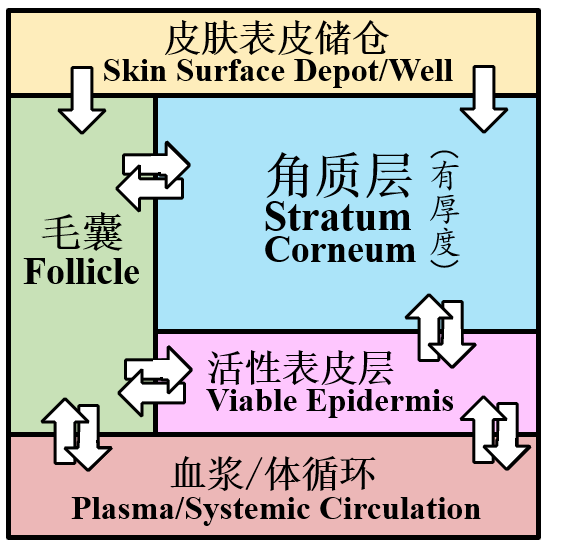
\includegraphics[scale=0.6]{./figs/p1.png}
  \caption{平行分层皮肤仓室的简化图解(箭头代表BPS的可能运输方向)}
  \label{分层皮肤}
\end{figure}

\begin{figure}[H]
  \centering
  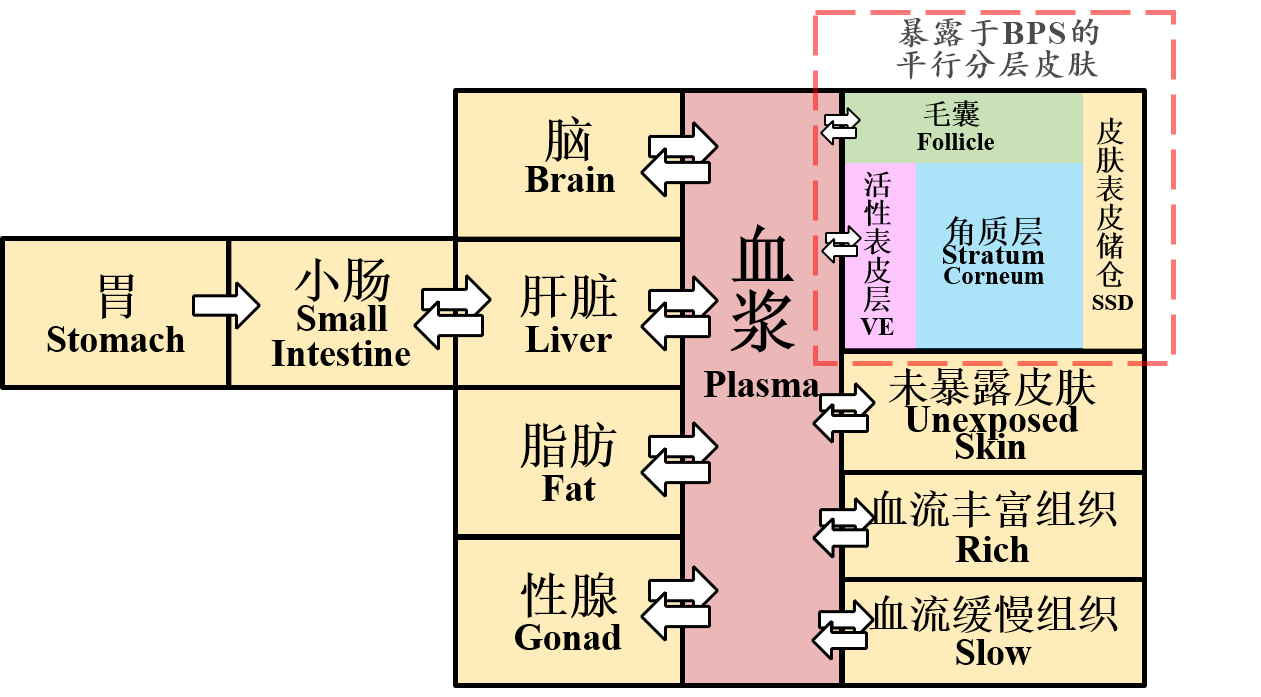
\includegraphics[scale=0.6]{./figs/p2.png}
  \caption{BPS人体内PBPK模型的简化图解(箭头代表BPS的可能运输方向)}
  \label{模型图解}
\end{figure}
\section{模型的数学形式}
本文中的PBPK模型共有个14仓室,包括:暴露皮肤\{皮肤表皮储仓, 角质层, 毛囊, 活性表皮层\}, 胃, 小肠, 未暴露于化学品的皮肤, 血浆, 脂肪, 性腺, 肝脏, 脑, 血流丰富组织, 血流缓慢组织.
其中暴露的含义为“在实验中与BPS接触”.
根据各仓室之间的关系以及BPS在各仓室内的生化反应, 得到19个解关于时间$t$变化的常微分方程与1个偏微分方程. 这些微分方程共同构成了BPS的带平行分层皮肤仓室的PBPK模型.  

\subsubsection*{角质层内BPS的浓度$\varphi(x,t)$}
如(\ref{eq0}), 其中的偏微分方程本质上是一个扩散对流方程,其解$\varphi$代表角质层(Stratum Corneum)中BPs含量, 自变量$x$代表角质层的深度, 自变量$t$代表时间, $DSC$代表BPS在角质层中的有效扩
散系数$(cm^2/h)$, $u_1$代表BPS随脱屑向皮肤表面转移的速度$(cm/min)$, $T_{SC}$代表角质层的深度$(um)$, $HSC_{well}$代表角质层和皮肤表皮储仓之间的分配系数, 
$C_{well}(t)$代表皮肤表皮储仓在$t$时刻的BPS浓度$(nmol/cm^3)$, $HSC_{VE}$代表角质层和活性表皮之间的分配系数, $C_{VE}(t)$代表活性表皮在$t$时刻的BPS浓度$(nmol/cm^2)$.

\begin{equation}\label{eq0}
  \left\{\begin{aligned}
    \frac{\partial \varphi(x,t) }{\partial t^2} &= DSC \frac{\partial^2 \varphi(x,t)}{\partial x^2} + u_1 \frac{\partial \varphi(x,t)}{\partial t}, && 0\leq x \geq T_{SC}, \quad t\geq 0\\
    \varphi(0,t) &= HSC_{well} \times C_{well}(t), &&t\geq 0\\
    \varphi(T_{SC},t) &= HSC_{VE} \times C_{VE}(t), &&t\geq 0\\
    \varphi(x,0) &= 0, &&0\leq x \geq T_{SC}\\
  \end{aligned}\right.
  \end{equation}
\noindent 使用空间离散化的办法, 将角质层视作一个长度为$T_{SC}$的线段, 将该线段等距分为$10$段, 共$11$个节点$\{x_i\}_{0\leq i\leq 10}$. 其中第一个节点$x_0$视作皮肤表皮储仓, 最后一个节点$x_{10}$视作活性表皮.
$x_1$至$x_9$九个节点处BPS浓度的一阶与二阶空间导数值通过中心差分法近似表示: 
\begin{equation}\label{eq1.1}
  \left\{\begin{aligned}
    \frac{\partial^2}{\partial x^2}\varphi(x_j, t) &\approx \frac{\varphi_{j+1}(t) - 2\varphi_j(t) + \varphi_{j-1}(t)}{(\Delta x)^2}\\
    \frac{\partial}{\partial x}\varphi(x_j, t) &\approx \frac{\varphi_{j+1}(t) - \varphi_{j-1}(t)}{2\Delta x}\\
  \end{aligned}\right.
  \end{equation}
  \noindent 整理后得到这九个节点处BPS浓度关于时间的一阶导数值如(\ref{eq1}), $i=2,3,\dots,8$与(\ref{eq2}),(\ref{eq3}).其中$SCDX = \frac{T_{SC}}{10}$, 
  $V_{well}$为暴露皮肤表面储仓沉积体积$(cm^3)$, $A_{well}(t)$为皮肤表皮储仓在$t$时刻的BPS含量$(nmol)$,$V_{TVE}$为暴露皮肤活性表皮层体积$(cm^3)$, $A_{VE}(t)$为活性表皮在$t$时刻的BPS含量$(nmol)$.
  节点$x_1$和$x_9$处的时间导数值与其他节点不同的原因是: 与它们相邻的部分涉及到皮肤的不同层室,需要利用BPS在不同层室组织间
  的分配系数来确定两个不同层室间BPS的转移情况. 
\begin{multline}\label{eq1}
  \frac{dC_{SCi}(t)}{dt}=\left(\frac{DSC}{SCDX^2} -\frac{u_1}{2 \times  SCDX}\right)C_{SCi-1}(t)-\frac{2 \times DSC}{SCDX^2}  C_{SCi}(t)\\
  +\left(\frac{DSC}{SCDX^2}+\frac{u_1}{2 \times  SCDX}\right)C_{SCi+1}(t).
\end{multline}

\begin{multline}\label{eq2}
  \frac{dC_{SC1}(t)}{dt}=\left(\frac{DSC \times  HSC_{well}}{V_{well}  \times  SCDX^2 }-\frac{u_1  \times  HSC_{well}}{V_{well}  \times  2 \times  SCDX}\right)A_{well}(t)   -\frac{2 \times DSC}{SCDX^2}  C_{SC1}(t)\\
  +\left(\frac{DSC}{SCDX^2}+\frac{u_1}{2 \times  SCDX}\right)C_{SC2}(t).
\end{multline}

\begin{multline}\label{eq3}
  \frac{dC_{SC9}(t)}{dt}=\left(\frac{DSC}{SCDX^2} -\frac{u_1}{2 \times  SCDX}\right)C_{SC8}(t)-\frac{2 \times DSC}{SCDX^2}  C_{SC9}(t)\\
  +\left(\frac{DSC \times  HSC_{VE}}{V_{TVE}  \times  SCDX^2 }-\frac{u_1  \times  HSC_{VE}}{V_{TVE}  \times  2 \times  SCDX}\right)A_{VE}(t) .
\end{multline}

接下来介绍模型中余下的19个解关于时间$t$变化的常微分方程, 此部分内方程中出现的变量与常量的含义详情见附录\ref{app:B}.
\subsubsection*{毛囊内BPS的含量$A_{Fo}(t)$}
见(\ref{eq10}), 方程等式两端为$A_{Fo}(t)$的一阶导数. 在该PBPK模型中, 毛囊与皮肤表皮储仓和血液之间有着直接的物质交换, 故毛囊内BPS含量的增减与表皮储仓或血浆中BPS的含量有关, BPS在宏观上遵循着顺浓度梯度运输的
规则在不同组织内交换. 同时, 毛囊内BPS含量的增减会受到自身的限制, 当毛囊内BPS浓度高于血浆或表皮储仓中BPS浓度时, BPS会顺浓度梯度进入浓度小的组织.
\begin{multline}\label{eq10}
  \frac{dA_{Fo}(t)}{dt} = -\left(\frac{Pfo \times  AEXP \times  FEXP}{V_{TFo}  \times  HFo_{well} }
  +\frac{Qskin \times  AEXP \times  0.25}{BSA \times  V_{TFo}  \times  pskin}\right)A_{Fo}(t)\\
  +\frac{Pfo \times  AEXP \times  FEXP}{V_{well}  }A_{well}(t)+\frac{Qskin \times  AEXP \times  0.25}{BSA \times  V_{plasma}} A_{plasma}(t).
\end{multline}

\subsubsection*{皮肤表皮储仓内BPS的含量$A_{well}(t)$}
见(\ref{eq11}), 方程等式两端为$A_{well}(t)$的一阶导数. 类似(\ref{eq10}), 等式右端表现出了表皮储仓与节点$x_1$处的角质层和毛囊之间的顺浓度梯度物质交换关系. 同时, 皮肤表皮储存作为在实验
中直接和外源BPS接触的部位, 它要接受一个剂量为$f_1 (t)$(单位:nmol)的持续的外源BPS输入. 当$t>Time_{add}=\frac{1}{6}h$时, 皮肤停止接触外源BPS, $f_1 (t)=0$. 
等式右端有一个因数$ON(t)$, 当$t\leq Time_{expose}=\frac{13}{6}h$时, $ON(t)=1$, 皮肤处于BPS暴露状态;当$t> Time_{expose}$时, $ON(t)=0$, 暴露过BPS的皮肤被彻底清洗, 表皮储仓清空, 后续$A_{well}(t)$的值与一阶
导数值都为0.
\begin{multline}\label{eq11}
  \frac{dA_{well}(t)}{dt} = \left(\frac{DSC \times  AEXP \times  (1-FEXP)}{SCDX} C_{SC1}(t)-\frac{Pfo \times  AEXP \times  FEXP}{V_{TFo} \times  HFo_{well}} A_{Fo}(t)\right.\\
  \left. -\left(\left(\frac{DSC \times  HSC_{well}}{V_{well} \times  SCDX}-\frac{u_1 \times  HSC_{well}}{V_{well} }\right) \times  AEXP \times  (1-FEXP) \right.\right.\\
  \left.\left.-\frac{Pfo \times  AEXP \times  FEXP}{V_{well}} \right)A_{well}(t)+f_1 (t) \right) \times  ON(t).
\end{multline}

\subsubsection*{活性表皮层内BPS的含量$A_{VE}(t)$}
见(\ref{eq12}), 方程等式两端为$A_{VE}(t)$的一阶导数. 类似(\ref{eq10}), 等式右端表现出了活性表皮层与节点$x_9$处的角质层, 毛囊和血浆之间的顺浓度梯度物质交换关系. 
\begin{multline}\label{eq12}
  \frac{dA_{VE}(t)}{dt}=\frac{DSC \times  AEXP \times  (1-FEXP)}{SCDX} C_{SC9}(t)+\left(\left(\frac{-DSC \times  HSC_{VE}}{V_{TVE}  \times  SCDX}-\frac{u_1  \times  HSC_{VE}}{V_{TVE} }\right)\times \right.\\ 
   \left.AEXP \times  (1-FEXP)-\frac{Qskin \times  AEXP \times  0.75}{BSA \times  V_{TVE}  \times  pskin}\right)A_{VE}(t)+\frac{Qskin \times  AEXP \times  0.75}{BSA \times  V_{plasma} } A_{plasma}(t).
\end{multline}

\subsubsection*{胃部BPS的含量$A_{ST}(t)$}
见(\ref{eq13}), 方程等式两端为$A_{ST}(t)$的一阶导数. 等式右端的第一个加数代表胃部BPS向肝脏和小肠转移的过程, 第二个加数是剂量为$f_2 (t)$(单位:nmol)的通过口服吸收的外源BPS. 但由于本文不考虑
口服吸收BPS的情形, $f_2 (t)\equiv 0$, 可认为胃部内始终不含有BPS或它的衍生物.
\begin{equation}\label{eq13}
  \frac{dA_{ST}(t)}{dt}=-(k_0+ge)A_{ST}(t)+f_2 (t).
\end{equation}
\subsubsection*{未暴露于BPS的皮肤, 脂肪, 性腺, 脑部, 血流丰富组织, 血流缓慢组织的BPS的含量}
见(\ref{eq14})至(\ref{eq20}), 各方程的等式两端为小标题中组织器官内BPS含量的一阶导数. 这些等式的右端一致地代表了对应组织器官与血浆之间的顺浓度梯度物质交换关系. 
\begin{multline}\label{eq14}
  \frac{dA_{skin}(t)}{dt}=\frac{-Qskin \times  (1-\frac{AEXP}{BSA})}{(V_{skin}-V_{TSC}-V_{TVE}-V_{TFo}) \times  pskin} A_{skin}(t)+\frac{Qskin \times  (1-\frac{AEXP}{BSA})}{V_{plasma}}  A_{plasma}(t).
\end{multline}

\begin{equation}\label{eq15}
  \frac{dA_{fat}(t)}{dt}=\frac{-Qfat}{V_{fat}  \times  pfat} A_{fat}(t)+\frac{Qfat}{V_{plasma}}  A_{plasma}(t).
\end{equation}

\begin{equation}\label{eq16}
  \frac{dA_{gonad}(t)}{dt}=\frac{-Qgonad}{V_{gonad}  \times  pgonad} A_{gonad}(t)+\frac{Qgonad}{V_{plasma}}  A_{plasma}(t).
\end{equation}

\begin{equation}\label{eq18}
  \frac{dA_{brain}(t)}{dt}=\frac{-Qbrain}{V_{brain}  \times  pbrain} A_{brain}(t)+\frac{Qbrain}{V_{plasma}}  A_{plasma}(t).
\end{equation}

\begin{equation}\label{eq19}
  \frac{dA_{rich}(t)}{dt}=\frac{-Qrich}{V_{rich}  \times  prich} A_{rich}(t)+\frac{Qrich}{V_{plasma}}  A_{plasma}(t).
\end{equation}

\begin{equation}\label{eq20}
  \frac{dA_{slow}(t)}{dt}=\frac{-Qslow}{V_{slow}  \times  pslow} A_{slow}(t)+\frac{Qslow}{V_{plasma}}  A_{plasma}(t).
\end{equation}

\subsubsection*{血浆内的BPS的含量}
见(\ref{eq17}), 方程等式两端为血浆内BPS含量的一阶导数. 血浆是体循环的重要组成部分, 该PBPK模型内的各仓室由血浆连接起来, 几乎每个仓室都与血浆有直接的物质交换, BPS从组织器官内进入血浆, 血浆又
携带着BPS进入各个组织器官. 等式的右端代表了血浆与毛囊, 活性表皮层, 未直接暴露于BPS的皮肤组织, 脂肪, 性腺, 脑部, 血流丰富组织, 血流缓慢组织, 肝脏之间的顺浓度梯度物质交换关系. 
等式右端除了$A_{plasma}(t)$项外每一项都有因数$Qc-Kurinebps$, 其中$Qc$是心脏血流速度$(L/h)$, $Kurinebps$是BPS的尿液排泄参数$(L/h)$, 它们相减代表了每轮血液循环净剩的携带了BPS的血浆量.
\begin{multline}\label{eq17}
  \frac{dA_{plasma}(t)}{dt}=\frac{(Qc-Kurinebps) \times  Qskin \times  \frac{AEXP}{BSA} \times  0.25}{Qc \times  V_{TFo}  \times  pskin} A_{Fo}(t)\\
  +\frac{(Qc-Kurinebps) \times  Qskin \times  \frac{AEXP}{BSA} \times  0.75}{Qc \times  V_{TVE}  \times  pskin} A_{VE}(t)\\
  +\frac{(Qc-Kurinebps) \times  Qskin \times  (1-\frac{AEXP}{BSA})}{Qc \times  (V_{skin}-V_{TSC}-V_{TVE}-V_{TFo}) \times  pskin} A_{skin}(t)\\
  +\frac{(Qc-Kurinebps) \times  Qfat}{Qc \times  V_{fat}  \times  pfat} A_{fat}(t)
  +\frac{(Qc-Kurinebps) \times  Qgonad}{Qc \times  V_{gonad}  \times  pgonad} A_{gonad}(t)\\
  -\frac{Qc}{V_{plasma}}  A_{plasma}(t)+\frac{(Qc-Kurinebps) \times  Qbrain}{Qc \times  V_{brain} \times  pbrain} A_{brain}(t)\\
  +\frac{(Qc-Kurinebps) \times  Qrich}{Qc \times  V_{rich}  \times  prich} A_{rich}(t)
  +\frac{(Qc-Kurinebps) \times  Qslow}{Qc \times  V_{slow}  \times  pslow} A_{slow}(t)\\
  +\frac{(Qc-Kurinebps) \times  Qliver}{Qc \times  V_{liver} \times  pliver} A_{liver}(t).
\end{multline}

\subsubsection*{胃肠部的BPS-g的含量$A_{GIBPSg}(t)$与胃肠部的BPS-s的含量$A_{GIBPSs}(t)$}
见(\ref{eq21}), 方程等式两端为胃肠部的BPS-g的含量的一阶导数. 等式右端的第二个加数代表了小肠内的BPS葡萄苷酸化为BPS-g的过程, 第一个加数代表了BPS-g从胃肠部进入血液的过程. 
在本文中, 没有口服吸收途径, 认为胃肠部不存在BPS-g或BPS-s. 对于(\ref{eq22})有类似的说明, 不同在于小肠内几乎不发生BPS硫酸盐化为BPS-s的反应.
\begin{equation}\label{eq21}
  \frac{dA_{GIBPSg}(t)}{dt}=-kGIing \times  A_{GIBPSg}(t)+\frac{Vmaxgutg \times  A_{SI}(t)}{enterocytes \times  Kmgutg+A_{SI}(t)+\frac{A_{SI}(t)^2}{enterocytes \times  Ksigutg}}.
\end{equation}

\begin{equation}\label{eq22}
  \frac{dA_{GIBPSs}(t)}{dt}=-kGIins \times  A_{GIBPSs}(t)+\frac{Vmaxguts \times  A_{SI}(t)}{enterocytes \times  Kmguts+A_{SI}(t)}.
\end{equation}
\subsubsection*{小肠的BPS的含量$A_{SI}(t)$}
见(\ref{eq23}), 方程等式两端为小肠的BPS的含量的一阶导数. 等式右端的第一个加数代表了口服BPS时胃部BPS进入小肠的过程, 第二个加数代表了小肠内部分BPS进入肝脏的过程, 后两个加数代表了部分BPS在小肠内葡萄苷酸化为BPS-g与硫酸盐化为BPS-s的反应过程
(小肠内几乎不发生BPS磷酸盐化反应, 此处对应的最大反应速率$Vmaxguts$非常小). 
在本文中, 没有口服吸收BPS的途径, 认为小肠内不存在BPS及其衍生物. 
\begin{multline}\label{eq23}
  \frac{dA_{SI}(t)}{dt}=ge \times  A_{ST}(t)-k1 \times  A_{SI}(t)-\frac{Vmaxgutg \times  A_{SI}(t)}{enterocytes \times  Kmgutg+A_{SI}(t)+\frac{A_{SI}(t)^2}{enterocytes \times  Ksigutg}}\\
  -\frac{Vmaxguts \times  A_{SI}(t)}{enterocytes \times  Kmguts+A_{SI}(t)}.
\end{multline}
\subsubsection*{肝脏的BPS的含量$A_{liver}(t)$}
见(\ref{eq24}), 方程等式两端为肝脏的BPS的含量的一阶导数. 等式右端的前两个加数分别代表了口服BPS时胃部和小肠内BPS进入肝脏的过程, 第三第四个加数代表了肝脏与血浆之间的顺浓度梯度物质交换关系, 第五第六个加数代表了
BPS-g与BPS-s引起肝脏内部分BPS发生肝肠循环的过程, 后两个加数代表了部分BPS在肝脏内葡萄苷酸化为BPS-g与硫酸盐化为BPS-s的反应过程. 
\begin{multline}\label{eq24}
  \frac{dA_{liver}(t)}{dt}=k0 \times  A_{ST}(t)+k1 \times  A_{SI}(t)+\frac{Qliver}{V_{plasma} } A_{plasma}(t)-\frac{Qliver}{V_{liver}  \times  pliver} A_{liver}(t)\\
  +kenterobpsg \times  A_{BPSg\_delay}(t)+kenterobpss \times  A_{BPSs\_delay}(t)\\
  -\frac{Vmaxliverg \times  A_{liver}(t)}{V_{liver}  \times  pliver \times  Kmliverg+A_{liver}(t)}-\frac{Vmaxlivers \times  A_{liver}(t)}{V_{liver}  \times  pliver \times  Kmlivers+A_{liver}(t)}.
\end{multline}

\subsubsection*{发生肝肠循环/小肠内的BPS-g/BPS-s的量$A_{BPSg\_delay}(t)$/$A_{BPSs\_delay}(t)$}
见(\ref{eq25}), 方程等式两端为发生肝肠循环的BPS-g的量的一阶导数. 等式右端的第一个加数代表了胃肠部BPS-g进入血浆后再进入肝肠循环的过程,第二个加数代表了肝肠循环中的BPS-g进入血液循环的过程, 最后一个加数
代表了肝脏中BPS新转化成的BPS-g进入肝肠循环的过程. 对于发生肝肠循环的BPS-s的量的方程(\ref{eq26}), 有着完全一致的描述.
\begin{multline}\label{eq25}
  \frac{dA_{BPSg\_delay}(t)}{dt}=met2g \times  kGIing \times  A_{GIBPSg}(t)\\
  -(kentero+k4_{IV}+kenterobpsg) \times  A_{BPSg\_delay}(t)
  +\frac{met2g \times  Vmaxliverg \times  A_{liver}(t)}{V_{liver}  \times  pliver \times  Kmliverg+A_{liver}(t)}.
\end{multline}

\begin{multline}\label{eq26}
  \frac{dA_{BPSs\_delay}(t)}{dt}=met2s \times  kGIins \times  A_{GIBPSs}(t)\\
  -(kentero+k4_{IV}+kenterobpss) \times  A_{BPSs\_delay}(t)
  +\frac{met2s \times  Vmaxlivers \times  A_{liver}(t)}{V_{liver}  \times  pliver \times  Kmlivers+A_{liver}(t)}.
\end{multline}

\subsubsection*{人体内BPS-g/BPS-s的总含量$A_{BPSg}(t)$/$A_{BPSs}(t)$}
见(\ref{eq27}), 方程等式两端为人体内BPS-g的总含量的一阶导数. 等式右端的第一个加数代表了口服摄入BPS时, 胃肠部产生的BPS-g进入血液后未进入肝肠循环的部分BPS-g, 第二个加数代表了正在进行肝肠循环的BPS-g, 第三个
加数代表了BPS-g随尿液排出人体的过程, 最后一个加数代表了BPS通过肝脏转化成的BPS-g进入血液后未进入肝肠循环的部分BPS-g.(\ref{eq28})与之相似.

\begin{multline}\label{eq27}
  \frac{dA_{BPSg}(t)}{dt}=met1g \times  kGIing \times  A_{GIBPSg}(t)+kentero \times  A_{BPSg\_delay}(t)-\frac{Kurinebpsg}{Vbodyg+10^{-34} } A_{BPSg}(t)\\
  +\frac{met1g \times  Vmaxliverg \times  A_{liver}(t)}{V_{liver}  \times  pliver \times  Kmliverg+A_{liver}(t)}.
\end{multline}

\begin{multline}\label{eq28}
  \frac{dA_{BPSs}(t)}{dt}=met1s \times  kGIins \times  A_{GIBPSs}(t)+kentero \times  A_{BPSs\_delay}(t)-\frac{Kurinebpss}{Vbodys+10^{-34}} A_{BPSs}(t)\\
  +\frac{met1s \times  Vmaxlivers \times  A_{liver}(t)}{V_{liver}  \times  pliver \times  Kmlivers+A_{liver}(t)}.
\end{multline}

综上, 本文的PBPK模型的数学形式的主要部分为一个由28个常微分方程构成的微分方程组, 其中每个方程的解关于时间$t$变化, 且每个解的初值都是0.
除此之外, 根据实验过程, 还需计算尿液中的BPS与BPS-g的在$t$时刻的含量$A_{urinebps}(t)$与$A_{urinebpsg}(t)$, (\ref{eq29})与(\ref{eq30})给出了它们的一阶导数值.
这两个等式都不是常微分方程.
\begin{multline}\label{eq29}
  \frac{dA_{urinebps}(t)}{dt}=Kurinebps\times \left(\frac{  Qskin \times  \frac{AEXP}{BSA} \times  0.25}{Qc \times  V_{TFo}  \times  pskin} A_{Fo}(t)
  +\frac{  Qskin \times  \frac{AEXP}{BSA} \times  0.75}{Qc \times  V_{TVE}  \times  pskin} A_{VE}(t)\right.\\
  \left.+\frac{  Qskin \times  (1-\frac{AEXP}{BSA})}{Qc \times  (V_{skin}-V_{TSC}-V_{TVE}-V_{TFo}) \times  pskin} A_{skin}(t)\right.\\
  \left.+\frac{  Qfat}{Qc \times  V_{fat}  \times  pfat} A_{fat}(t)
  +\frac{  Qgonad}{Qc \times  V_{gonad}  \times  pgonad} A_{gonad}(t)\right.\\
  \left.+\frac{  Qbrain}{Qc \times  V_{brain} \times  pbrain} A_{brain}(t)
  +\frac{  Qrich}{Qc \times  V_{rich}  \times  prich} A_{rich}(t)\right.\\
  \left.+\frac{  Qslow}{Qc \times  V_{slow}  \times  pslow} A_{slow}(t)
  +\frac{  Qliver}{Qc \times  V_{liver} \times  pliver} A_{liver}(t)\right).
\end{multline}

\begin{equation}\label{eq30}
  \frac{dA_{urinebpsg}(t)}{dt}=\frac{Kurinebpsg}{Vbodyg+10^{-34} } A_{BPSg}(t).
\end{equation}
\section{PBPK模型的求解}
确定模型的数学形式后, 将Hu等人\cite{12}提供的数据相对应地代入至方程的各个参数, 使用Python中的第三方库函数scipy.integrate.odeint()对
微分方程组求解, 该函数默认使用LSODA数值格式. LSODA是一种高效的支持自适应步长的算法\cite{14}, 根据设置好的误差限度, 若按照原有的预设步长来进行下一节点的数值计算, 得到的误差大于限度, 则将此步预设步长拆分为更小的多个步长, 
以此来减小误差至限度以内; 若按照预设步长计算时得到的误差远小于限度, 则适当增大步长以减小资源消耗. 同时, LSODA同时支持刚性与非刚性问题, 处理刚性问题时, 它使用后向微分公式(BDF),处理非刚性问题时, 它使用Runge-Kutta公式.

根据Hu等人\cite{11}的实验, 每个解的初值都设置为0, 时间网格设置为$range(0,75,0.005)$, 时间步长为$0.005h$, 共$15000$个时间节点.
每个方程的解都对应了一条人体某组织器官内BPS(或BPS-g, BPS-s)的含量$(mmol)$或浓度$(mmol/L)$随时间变化的曲线.

\begin{figure}[H]
  \centering
  \begin{subfigure}{0.6\textwidth}
    \centering
    \resizebox{1\textwidth}{!}{%% Creator: Matplotlib, PGF backend
%%
%% To include the figure in your LaTeX document, write
%%   \input{<filename>.pgf}
%%
%% Make sure the required packages are loaded in your preamble
%%   \usepackage{pgf}
%%
%% Also ensure that all the required font packages are loaded; for instance,
%% the lmodern package is sometimes necessary when using math font.
%%   \usepackage{lmodern}
%%
%% Figures using additional raster images can only be included by \input if
%% they are in the same directory as the main LaTeX file. For loading figures
%% from other directories you can use the `import` package
%%   \usepackage{import}
%%
%% and then include the figures with
%%   \import{<path to file>}{<filename>.pgf}
%%
%% Matplotlib used the following preamble
%%   \def\mathdefault#1{#1}
%%   \everymath=\expandafter{\the\everymath\displaystyle}
%%   
%%   \usepackage{fontspec}
%%   \setmainfont{DejaVuSerif.ttf}[Path=\detokenize{C:/Users/许先生/AppData/Local/Programs/Python/Python310/Lib/site-packages/matplotlib/mpl-data/fonts/ttf/}]
%%   \setsansfont{simhei.ttf}[Path=\detokenize{C:/Windows/Fonts/}]
%%   \setmonofont{DejaVuSansMono.ttf}[Path=\detokenize{C:/Users/许先生/AppData/Local/Programs/Python/Python310/Lib/site-packages/matplotlib/mpl-data/fonts/ttf/}]
%%   \makeatletter\@ifpackageloaded{underscore}{}{\usepackage[strings]{underscore}}\makeatother
%%
\begingroup%
\makeatletter%
\begin{pgfpicture}%
\pgfpathrectangle{\pgfpointorigin}{\pgfqpoint{15.360000in}{7.656000in}}%
\pgfusepath{use as bounding box, clip}%
\begin{pgfscope}%
\pgfsetbuttcap%
\pgfsetmiterjoin%
\definecolor{currentfill}{rgb}{1.000000,1.000000,1.000000}%
\pgfsetfillcolor{currentfill}%
\pgfsetlinewidth{0.000000pt}%
\definecolor{currentstroke}{rgb}{1.000000,1.000000,1.000000}%
\pgfsetstrokecolor{currentstroke}%
\pgfsetdash{}{0pt}%
\pgfpathmoveto{\pgfqpoint{0.000000in}{0.000000in}}%
\pgfpathlineto{\pgfqpoint{15.360000in}{0.000000in}}%
\pgfpathlineto{\pgfqpoint{15.360000in}{7.656000in}}%
\pgfpathlineto{\pgfqpoint{0.000000in}{7.656000in}}%
\pgfpathlineto{\pgfqpoint{0.000000in}{0.000000in}}%
\pgfpathclose%
\pgfusepath{fill}%
\end{pgfscope}%
\begin{pgfscope}%
\pgfsetbuttcap%
\pgfsetmiterjoin%
\definecolor{currentfill}{rgb}{1.000000,1.000000,1.000000}%
\pgfsetfillcolor{currentfill}%
\pgfsetlinewidth{0.000000pt}%
\definecolor{currentstroke}{rgb}{0.000000,0.000000,0.000000}%
\pgfsetstrokecolor{currentstroke}%
\pgfsetstrokeopacity{0.000000}%
\pgfsetdash{}{0pt}%
\pgfpathmoveto{\pgfqpoint{1.920000in}{0.842160in}}%
\pgfpathlineto{\pgfqpoint{13.824000in}{0.842160in}}%
\pgfpathlineto{\pgfqpoint{13.824000in}{6.737280in}}%
\pgfpathlineto{\pgfqpoint{1.920000in}{6.737280in}}%
\pgfpathlineto{\pgfqpoint{1.920000in}{0.842160in}}%
\pgfpathclose%
\pgfusepath{fill}%
\end{pgfscope}%
\begin{pgfscope}%
\pgfsetbuttcap%
\pgfsetroundjoin%
\definecolor{currentfill}{rgb}{0.000000,0.000000,0.000000}%
\pgfsetfillcolor{currentfill}%
\pgfsetlinewidth{0.803000pt}%
\definecolor{currentstroke}{rgb}{0.000000,0.000000,0.000000}%
\pgfsetstrokecolor{currentstroke}%
\pgfsetdash{}{0pt}%
\pgfsys@defobject{currentmarker}{\pgfqpoint{0.000000in}{-0.048611in}}{\pgfqpoint{0.000000in}{0.000000in}}{%
\pgfpathmoveto{\pgfqpoint{0.000000in}{0.000000in}}%
\pgfpathlineto{\pgfqpoint{0.000000in}{-0.048611in}}%
\pgfusepath{stroke,fill}%
}%
\begin{pgfscope}%
\pgfsys@transformshift{2.446642in}{0.842160in}%
\pgfsys@useobject{currentmarker}{}%
\end{pgfscope}%
\end{pgfscope}%
\begin{pgfscope}%
\definecolor{textcolor}{rgb}{0.000000,0.000000,0.000000}%
\pgfsetstrokecolor{textcolor}%
\pgfsetfillcolor{textcolor}%
\pgftext[x=2.446642in,y=0.744938in,,top]{\color{textcolor}{\sffamily\fontsize{10.000000}{12.000000}\selectfont\catcode`\^=\active\def^{\ifmmode\sp\else\^{}\fi}\catcode`\%=\active\def%{\%}0}}%
\end{pgfscope}%
\begin{pgfscope}%
\pgfsetbuttcap%
\pgfsetroundjoin%
\definecolor{currentfill}{rgb}{0.000000,0.000000,0.000000}%
\pgfsetfillcolor{currentfill}%
\pgfsetlinewidth{0.803000pt}%
\definecolor{currentstroke}{rgb}{0.000000,0.000000,0.000000}%
\pgfsetstrokecolor{currentstroke}%
\pgfsetdash{}{0pt}%
\pgfsys@defobject{currentmarker}{\pgfqpoint{0.000000in}{-0.048611in}}{\pgfqpoint{0.000000in}{0.000000in}}{%
\pgfpathmoveto{\pgfqpoint{0.000000in}{0.000000in}}%
\pgfpathlineto{\pgfqpoint{0.000000in}{-0.048611in}}%
\pgfusepath{stroke,fill}%
}%
\begin{pgfscope}%
\pgfsys@transformshift{3.891574in}{0.842160in}%
\pgfsys@useobject{currentmarker}{}%
\end{pgfscope}%
\end{pgfscope}%
\begin{pgfscope}%
\definecolor{textcolor}{rgb}{0.000000,0.000000,0.000000}%
\pgfsetstrokecolor{textcolor}%
\pgfsetfillcolor{textcolor}%
\pgftext[x=3.891574in,y=0.744938in,,top]{\color{textcolor}{\sffamily\fontsize{10.000000}{12.000000}\selectfont\catcode`\^=\active\def^{\ifmmode\sp\else\^{}\fi}\catcode`\%=\active\def%{\%}10}}%
\end{pgfscope}%
\begin{pgfscope}%
\pgfsetbuttcap%
\pgfsetroundjoin%
\definecolor{currentfill}{rgb}{0.000000,0.000000,0.000000}%
\pgfsetfillcolor{currentfill}%
\pgfsetlinewidth{0.803000pt}%
\definecolor{currentstroke}{rgb}{0.000000,0.000000,0.000000}%
\pgfsetstrokecolor{currentstroke}%
\pgfsetdash{}{0pt}%
\pgfsys@defobject{currentmarker}{\pgfqpoint{0.000000in}{-0.048611in}}{\pgfqpoint{0.000000in}{0.000000in}}{%
\pgfpathmoveto{\pgfqpoint{0.000000in}{0.000000in}}%
\pgfpathlineto{\pgfqpoint{0.000000in}{-0.048611in}}%
\pgfusepath{stroke,fill}%
}%
\begin{pgfscope}%
\pgfsys@transformshift{5.336506in}{0.842160in}%
\pgfsys@useobject{currentmarker}{}%
\end{pgfscope}%
\end{pgfscope}%
\begin{pgfscope}%
\definecolor{textcolor}{rgb}{0.000000,0.000000,0.000000}%
\pgfsetstrokecolor{textcolor}%
\pgfsetfillcolor{textcolor}%
\pgftext[x=5.336506in,y=0.744938in,,top]{\color{textcolor}{\sffamily\fontsize{10.000000}{12.000000}\selectfont\catcode`\^=\active\def^{\ifmmode\sp\else\^{}\fi}\catcode`\%=\active\def%{\%}20}}%
\end{pgfscope}%
\begin{pgfscope}%
\pgfsetbuttcap%
\pgfsetroundjoin%
\definecolor{currentfill}{rgb}{0.000000,0.000000,0.000000}%
\pgfsetfillcolor{currentfill}%
\pgfsetlinewidth{0.803000pt}%
\definecolor{currentstroke}{rgb}{0.000000,0.000000,0.000000}%
\pgfsetstrokecolor{currentstroke}%
\pgfsetdash{}{0pt}%
\pgfsys@defobject{currentmarker}{\pgfqpoint{0.000000in}{-0.048611in}}{\pgfqpoint{0.000000in}{0.000000in}}{%
\pgfpathmoveto{\pgfqpoint{0.000000in}{0.000000in}}%
\pgfpathlineto{\pgfqpoint{0.000000in}{-0.048611in}}%
\pgfusepath{stroke,fill}%
}%
\begin{pgfscope}%
\pgfsys@transformshift{6.781438in}{0.842160in}%
\pgfsys@useobject{currentmarker}{}%
\end{pgfscope}%
\end{pgfscope}%
\begin{pgfscope}%
\definecolor{textcolor}{rgb}{0.000000,0.000000,0.000000}%
\pgfsetstrokecolor{textcolor}%
\pgfsetfillcolor{textcolor}%
\pgftext[x=6.781438in,y=0.744938in,,top]{\color{textcolor}{\sffamily\fontsize{10.000000}{12.000000}\selectfont\catcode`\^=\active\def^{\ifmmode\sp\else\^{}\fi}\catcode`\%=\active\def%{\%}30}}%
\end{pgfscope}%
\begin{pgfscope}%
\pgfsetbuttcap%
\pgfsetroundjoin%
\definecolor{currentfill}{rgb}{0.000000,0.000000,0.000000}%
\pgfsetfillcolor{currentfill}%
\pgfsetlinewidth{0.803000pt}%
\definecolor{currentstroke}{rgb}{0.000000,0.000000,0.000000}%
\pgfsetstrokecolor{currentstroke}%
\pgfsetdash{}{0pt}%
\pgfsys@defobject{currentmarker}{\pgfqpoint{0.000000in}{-0.048611in}}{\pgfqpoint{0.000000in}{0.000000in}}{%
\pgfpathmoveto{\pgfqpoint{0.000000in}{0.000000in}}%
\pgfpathlineto{\pgfqpoint{0.000000in}{-0.048611in}}%
\pgfusepath{stroke,fill}%
}%
\begin{pgfscope}%
\pgfsys@transformshift{8.226370in}{0.842160in}%
\pgfsys@useobject{currentmarker}{}%
\end{pgfscope}%
\end{pgfscope}%
\begin{pgfscope}%
\definecolor{textcolor}{rgb}{0.000000,0.000000,0.000000}%
\pgfsetstrokecolor{textcolor}%
\pgfsetfillcolor{textcolor}%
\pgftext[x=8.226370in,y=0.744938in,,top]{\color{textcolor}{\sffamily\fontsize{10.000000}{12.000000}\selectfont\catcode`\^=\active\def^{\ifmmode\sp\else\^{}\fi}\catcode`\%=\active\def%{\%}40}}%
\end{pgfscope}%
\begin{pgfscope}%
\pgfsetbuttcap%
\pgfsetroundjoin%
\definecolor{currentfill}{rgb}{0.000000,0.000000,0.000000}%
\pgfsetfillcolor{currentfill}%
\pgfsetlinewidth{0.803000pt}%
\definecolor{currentstroke}{rgb}{0.000000,0.000000,0.000000}%
\pgfsetstrokecolor{currentstroke}%
\pgfsetdash{}{0pt}%
\pgfsys@defobject{currentmarker}{\pgfqpoint{0.000000in}{-0.048611in}}{\pgfqpoint{0.000000in}{0.000000in}}{%
\pgfpathmoveto{\pgfqpoint{0.000000in}{0.000000in}}%
\pgfpathlineto{\pgfqpoint{0.000000in}{-0.048611in}}%
\pgfusepath{stroke,fill}%
}%
\begin{pgfscope}%
\pgfsys@transformshift{9.671302in}{0.842160in}%
\pgfsys@useobject{currentmarker}{}%
\end{pgfscope}%
\end{pgfscope}%
\begin{pgfscope}%
\definecolor{textcolor}{rgb}{0.000000,0.000000,0.000000}%
\pgfsetstrokecolor{textcolor}%
\pgfsetfillcolor{textcolor}%
\pgftext[x=9.671302in,y=0.744938in,,top]{\color{textcolor}{\sffamily\fontsize{10.000000}{12.000000}\selectfont\catcode`\^=\active\def^{\ifmmode\sp\else\^{}\fi}\catcode`\%=\active\def%{\%}50}}%
\end{pgfscope}%
\begin{pgfscope}%
\pgfsetbuttcap%
\pgfsetroundjoin%
\definecolor{currentfill}{rgb}{0.000000,0.000000,0.000000}%
\pgfsetfillcolor{currentfill}%
\pgfsetlinewidth{0.803000pt}%
\definecolor{currentstroke}{rgb}{0.000000,0.000000,0.000000}%
\pgfsetstrokecolor{currentstroke}%
\pgfsetdash{}{0pt}%
\pgfsys@defobject{currentmarker}{\pgfqpoint{0.000000in}{-0.048611in}}{\pgfqpoint{0.000000in}{0.000000in}}{%
\pgfpathmoveto{\pgfqpoint{0.000000in}{0.000000in}}%
\pgfpathlineto{\pgfqpoint{0.000000in}{-0.048611in}}%
\pgfusepath{stroke,fill}%
}%
\begin{pgfscope}%
\pgfsys@transformshift{11.116234in}{0.842160in}%
\pgfsys@useobject{currentmarker}{}%
\end{pgfscope}%
\end{pgfscope}%
\begin{pgfscope}%
\definecolor{textcolor}{rgb}{0.000000,0.000000,0.000000}%
\pgfsetstrokecolor{textcolor}%
\pgfsetfillcolor{textcolor}%
\pgftext[x=11.116234in,y=0.744938in,,top]{\color{textcolor}{\sffamily\fontsize{10.000000}{12.000000}\selectfont\catcode`\^=\active\def^{\ifmmode\sp\else\^{}\fi}\catcode`\%=\active\def%{\%}60}}%
\end{pgfscope}%
\begin{pgfscope}%
\pgfsetbuttcap%
\pgfsetroundjoin%
\definecolor{currentfill}{rgb}{0.000000,0.000000,0.000000}%
\pgfsetfillcolor{currentfill}%
\pgfsetlinewidth{0.803000pt}%
\definecolor{currentstroke}{rgb}{0.000000,0.000000,0.000000}%
\pgfsetstrokecolor{currentstroke}%
\pgfsetdash{}{0pt}%
\pgfsys@defobject{currentmarker}{\pgfqpoint{0.000000in}{-0.048611in}}{\pgfqpoint{0.000000in}{0.000000in}}{%
\pgfpathmoveto{\pgfqpoint{0.000000in}{0.000000in}}%
\pgfpathlineto{\pgfqpoint{0.000000in}{-0.048611in}}%
\pgfusepath{stroke,fill}%
}%
\begin{pgfscope}%
\pgfsys@transformshift{12.561166in}{0.842160in}%
\pgfsys@useobject{currentmarker}{}%
\end{pgfscope}%
\end{pgfscope}%
\begin{pgfscope}%
\definecolor{textcolor}{rgb}{0.000000,0.000000,0.000000}%
\pgfsetstrokecolor{textcolor}%
\pgfsetfillcolor{textcolor}%
\pgftext[x=12.561166in,y=0.744938in,,top]{\color{textcolor}{\sffamily\fontsize{10.000000}{12.000000}\selectfont\catcode`\^=\active\def^{\ifmmode\sp\else\^{}\fi}\catcode`\%=\active\def%{\%}70}}%
\end{pgfscope}%
\begin{pgfscope}%
\definecolor{textcolor}{rgb}{0.000000,0.000000,0.000000}%
\pgfsetstrokecolor{textcolor}%
\pgfsetfillcolor{textcolor}%
\pgftext[x=7.872000in,y=0.576535in,,top]{\color{textcolor}{\sffamily\fontsize{10.000000}{12.000000}\selectfont\catcode`\^=\active\def^{\ifmmode\sp\else\^{}\fi}\catcode`\%=\active\def%{\%}时间(h)}}%
\end{pgfscope}%
\begin{pgfscope}%
\pgfsetbuttcap%
\pgfsetroundjoin%
\definecolor{currentfill}{rgb}{0.000000,0.000000,0.000000}%
\pgfsetfillcolor{currentfill}%
\pgfsetlinewidth{0.803000pt}%
\definecolor{currentstroke}{rgb}{0.000000,0.000000,0.000000}%
\pgfsetstrokecolor{currentstroke}%
\pgfsetdash{}{0pt}%
\pgfsys@defobject{currentmarker}{\pgfqpoint{-0.048611in}{0.000000in}}{\pgfqpoint{-0.000000in}{0.000000in}}{%
\pgfpathmoveto{\pgfqpoint{-0.000000in}{0.000000in}}%
\pgfpathlineto{\pgfqpoint{-0.048611in}{0.000000in}}%
\pgfusepath{stroke,fill}%
}%
\begin{pgfscope}%
\pgfsys@transformshift{1.920000in}{1.110114in}%
\pgfsys@useobject{currentmarker}{}%
\end{pgfscope}%
\end{pgfscope}%
\begin{pgfscope}%
\definecolor{textcolor}{rgb}{0.000000,0.000000,0.000000}%
\pgfsetstrokecolor{textcolor}%
\pgfsetfillcolor{textcolor}%
\pgftext[x=1.406111in, y=1.062371in, left, base]{\color{textcolor}{\sffamily\fontsize{10.000000}{12.000000}\selectfont\catcode`\^=\active\def^{\ifmmode\sp\else\^{}\fi}\catcode`\%=\active\def%{\%}0.000%}}%
\end{pgfscope}%
\begin{pgfscope}%
\pgfsetbuttcap%
\pgfsetroundjoin%
\definecolor{currentfill}{rgb}{0.000000,0.000000,0.000000}%
\pgfsetfillcolor{currentfill}%
\pgfsetlinewidth{0.803000pt}%
\definecolor{currentstroke}{rgb}{0.000000,0.000000,0.000000}%
\pgfsetstrokecolor{currentstroke}%
\pgfsetdash{}{0pt}%
\pgfsys@defobject{currentmarker}{\pgfqpoint{-0.048611in}{0.000000in}}{\pgfqpoint{-0.000000in}{0.000000in}}{%
\pgfpathmoveto{\pgfqpoint{-0.000000in}{0.000000in}}%
\pgfpathlineto{\pgfqpoint{-0.048611in}{0.000000in}}%
\pgfusepath{stroke,fill}%
}%
\begin{pgfscope}%
\pgfsys@transformshift{1.920000in}{2.049146in}%
\pgfsys@useobject{currentmarker}{}%
\end{pgfscope}%
\end{pgfscope}%
\begin{pgfscope}%
\definecolor{textcolor}{rgb}{0.000000,0.000000,0.000000}%
\pgfsetstrokecolor{textcolor}%
\pgfsetfillcolor{textcolor}%
\pgftext[x=1.406111in, y=2.001403in, left, base]{\color{textcolor}{\sffamily\fontsize{10.000000}{12.000000}\selectfont\catcode`\^=\active\def^{\ifmmode\sp\else\^{}\fi}\catcode`\%=\active\def%{\%}0.002%}}%
\end{pgfscope}%
\begin{pgfscope}%
\pgfsetbuttcap%
\pgfsetroundjoin%
\definecolor{currentfill}{rgb}{0.000000,0.000000,0.000000}%
\pgfsetfillcolor{currentfill}%
\pgfsetlinewidth{0.803000pt}%
\definecolor{currentstroke}{rgb}{0.000000,0.000000,0.000000}%
\pgfsetstrokecolor{currentstroke}%
\pgfsetdash{}{0pt}%
\pgfsys@defobject{currentmarker}{\pgfqpoint{-0.048611in}{0.000000in}}{\pgfqpoint{-0.000000in}{0.000000in}}{%
\pgfpathmoveto{\pgfqpoint{-0.000000in}{0.000000in}}%
\pgfpathlineto{\pgfqpoint{-0.048611in}{0.000000in}}%
\pgfusepath{stroke,fill}%
}%
\begin{pgfscope}%
\pgfsys@transformshift{1.920000in}{2.988179in}%
\pgfsys@useobject{currentmarker}{}%
\end{pgfscope}%
\end{pgfscope}%
\begin{pgfscope}%
\definecolor{textcolor}{rgb}{0.000000,0.000000,0.000000}%
\pgfsetstrokecolor{textcolor}%
\pgfsetfillcolor{textcolor}%
\pgftext[x=1.406111in, y=2.940436in, left, base]{\color{textcolor}{\sffamily\fontsize{10.000000}{12.000000}\selectfont\catcode`\^=\active\def^{\ifmmode\sp\else\^{}\fi}\catcode`\%=\active\def%{\%}0.004%}}%
\end{pgfscope}%
\begin{pgfscope}%
\pgfsetbuttcap%
\pgfsetroundjoin%
\definecolor{currentfill}{rgb}{0.000000,0.000000,0.000000}%
\pgfsetfillcolor{currentfill}%
\pgfsetlinewidth{0.803000pt}%
\definecolor{currentstroke}{rgb}{0.000000,0.000000,0.000000}%
\pgfsetstrokecolor{currentstroke}%
\pgfsetdash{}{0pt}%
\pgfsys@defobject{currentmarker}{\pgfqpoint{-0.048611in}{0.000000in}}{\pgfqpoint{-0.000000in}{0.000000in}}{%
\pgfpathmoveto{\pgfqpoint{-0.000000in}{0.000000in}}%
\pgfpathlineto{\pgfqpoint{-0.048611in}{0.000000in}}%
\pgfusepath{stroke,fill}%
}%
\begin{pgfscope}%
\pgfsys@transformshift{1.920000in}{3.927211in}%
\pgfsys@useobject{currentmarker}{}%
\end{pgfscope}%
\end{pgfscope}%
\begin{pgfscope}%
\definecolor{textcolor}{rgb}{0.000000,0.000000,0.000000}%
\pgfsetstrokecolor{textcolor}%
\pgfsetfillcolor{textcolor}%
\pgftext[x=1.406111in, y=3.879468in, left, base]{\color{textcolor}{\sffamily\fontsize{10.000000}{12.000000}\selectfont\catcode`\^=\active\def^{\ifmmode\sp\else\^{}\fi}\catcode`\%=\active\def%{\%}0.006%}}%
\end{pgfscope}%
\begin{pgfscope}%
\pgfsetbuttcap%
\pgfsetroundjoin%
\definecolor{currentfill}{rgb}{0.000000,0.000000,0.000000}%
\pgfsetfillcolor{currentfill}%
\pgfsetlinewidth{0.803000pt}%
\definecolor{currentstroke}{rgb}{0.000000,0.000000,0.000000}%
\pgfsetstrokecolor{currentstroke}%
\pgfsetdash{}{0pt}%
\pgfsys@defobject{currentmarker}{\pgfqpoint{-0.048611in}{0.000000in}}{\pgfqpoint{-0.000000in}{0.000000in}}{%
\pgfpathmoveto{\pgfqpoint{-0.000000in}{0.000000in}}%
\pgfpathlineto{\pgfqpoint{-0.048611in}{0.000000in}}%
\pgfusepath{stroke,fill}%
}%
\begin{pgfscope}%
\pgfsys@transformshift{1.920000in}{4.866243in}%
\pgfsys@useobject{currentmarker}{}%
\end{pgfscope}%
\end{pgfscope}%
\begin{pgfscope}%
\definecolor{textcolor}{rgb}{0.000000,0.000000,0.000000}%
\pgfsetstrokecolor{textcolor}%
\pgfsetfillcolor{textcolor}%
\pgftext[x=1.406111in, y=4.818500in, left, base]{\color{textcolor}{\sffamily\fontsize{10.000000}{12.000000}\selectfont\catcode`\^=\active\def^{\ifmmode\sp\else\^{}\fi}\catcode`\%=\active\def%{\%}0.008%}}%
\end{pgfscope}%
\begin{pgfscope}%
\pgfsetbuttcap%
\pgfsetroundjoin%
\definecolor{currentfill}{rgb}{0.000000,0.000000,0.000000}%
\pgfsetfillcolor{currentfill}%
\pgfsetlinewidth{0.803000pt}%
\definecolor{currentstroke}{rgb}{0.000000,0.000000,0.000000}%
\pgfsetstrokecolor{currentstroke}%
\pgfsetdash{}{0pt}%
\pgfsys@defobject{currentmarker}{\pgfqpoint{-0.048611in}{0.000000in}}{\pgfqpoint{-0.000000in}{0.000000in}}{%
\pgfpathmoveto{\pgfqpoint{-0.000000in}{0.000000in}}%
\pgfpathlineto{\pgfqpoint{-0.048611in}{0.000000in}}%
\pgfusepath{stroke,fill}%
}%
\begin{pgfscope}%
\pgfsys@transformshift{1.920000in}{5.805275in}%
\pgfsys@useobject{currentmarker}{}%
\end{pgfscope}%
\end{pgfscope}%
\begin{pgfscope}%
\definecolor{textcolor}{rgb}{0.000000,0.000000,0.000000}%
\pgfsetstrokecolor{textcolor}%
\pgfsetfillcolor{textcolor}%
\pgftext[x=1.406111in, y=5.757532in, left, base]{\color{textcolor}{\sffamily\fontsize{10.000000}{12.000000}\selectfont\catcode`\^=\active\def^{\ifmmode\sp\else\^{}\fi}\catcode`\%=\active\def%{\%}0.010%}}%
\end{pgfscope}%
\begin{pgfscope}%
\definecolor{textcolor}{rgb}{0.000000,0.000000,0.000000}%
\pgfsetstrokecolor{textcolor}%
\pgfsetfillcolor{textcolor}%
\pgftext[x=1.350556in,y=3.789720in,,bottom,rotate=90.000000]{\color{textcolor}{\sffamily\fontsize{10.000000}{12.000000}\selectfont\catcode`\^=\active\def^{\ifmmode\sp\else\^{}\fi}\catcode`\%=\active\def%{\%}与前人的数值求解结果的相对误差}}%
\end{pgfscope}%
\begin{pgfscope}%
\pgfpathrectangle{\pgfqpoint{1.920000in}{0.842160in}}{\pgfqpoint{11.904000in}{5.895120in}}%
\pgfusepath{clip}%
\pgfsetrectcap%
\pgfsetroundjoin%
\pgfsetlinewidth{1.505625pt}%
\definecolor{currentstroke}{rgb}{0.121569,0.466667,0.705882}%
\pgfsetstrokecolor{currentstroke}%
\pgfsetdash{}{0pt}%
\pgfpathmoveto{\pgfqpoint{2.461091in}{1.356342in}}%
\pgfpathlineto{\pgfqpoint{2.461813in}{1.136661in}}%
\pgfpathlineto{\pgfqpoint{2.463981in}{2.346340in}}%
\pgfpathlineto{\pgfqpoint{2.464703in}{2.113707in}}%
\pgfpathlineto{\pgfqpoint{2.465426in}{3.173737in}}%
\pgfpathlineto{\pgfqpoint{2.466148in}{1.263779in}}%
\pgfpathlineto{\pgfqpoint{2.466871in}{1.290932in}}%
\pgfpathlineto{\pgfqpoint{2.467593in}{1.148560in}}%
\pgfpathlineto{\pgfqpoint{2.468316in}{1.399252in}}%
\pgfpathlineto{\pgfqpoint{2.469761in}{4.486894in}}%
\pgfpathlineto{\pgfqpoint{2.470483in}{1.665427in}}%
\pgfpathlineto{\pgfqpoint{2.471205in}{3.447999in}}%
\pgfpathlineto{\pgfqpoint{2.472650in}{1.372253in}}%
\pgfpathlineto{\pgfqpoint{2.473373in}{1.507185in}}%
\pgfpathlineto{\pgfqpoint{2.474095in}{1.138428in}}%
\pgfpathlineto{\pgfqpoint{2.474818in}{1.282562in}}%
\pgfpathlineto{\pgfqpoint{2.475540in}{1.113832in}}%
\pgfpathlineto{\pgfqpoint{2.476263in}{1.256588in}}%
\pgfpathlineto{\pgfqpoint{2.476985in}{1.215250in}}%
\pgfpathlineto{\pgfqpoint{2.478430in}{1.114927in}}%
\pgfpathlineto{\pgfqpoint{2.479153in}{1.125371in}}%
\pgfpathlineto{\pgfqpoint{2.479875in}{1.122396in}}%
\pgfpathlineto{\pgfqpoint{2.480597in}{1.114492in}}%
\pgfpathlineto{\pgfqpoint{2.482042in}{1.138230in}}%
\pgfpathlineto{\pgfqpoint{2.482765in}{1.115120in}}%
\pgfpathlineto{\pgfqpoint{2.483487in}{1.128681in}}%
\pgfpathlineto{\pgfqpoint{2.484932in}{1.114756in}}%
\pgfpathlineto{\pgfqpoint{2.485655in}{1.113862in}}%
\pgfpathlineto{\pgfqpoint{2.487100in}{1.127541in}}%
\pgfpathlineto{\pgfqpoint{2.487822in}{1.122369in}}%
\pgfpathlineto{\pgfqpoint{2.488545in}{1.119785in}}%
\pgfpathlineto{\pgfqpoint{2.489267in}{1.124603in}}%
\pgfpathlineto{\pgfqpoint{2.490712in}{1.115266in}}%
\pgfpathlineto{\pgfqpoint{2.491434in}{1.114384in}}%
\pgfpathlineto{\pgfqpoint{2.492157in}{1.125068in}}%
\pgfpathlineto{\pgfqpoint{2.492879in}{1.110958in}}%
\pgfpathlineto{\pgfqpoint{2.493602in}{1.112543in}}%
\pgfpathlineto{\pgfqpoint{2.494324in}{1.124694in}}%
\pgfpathlineto{\pgfqpoint{2.495047in}{1.115812in}}%
\pgfpathlineto{\pgfqpoint{2.496492in}{1.146255in}}%
\pgfpathlineto{\pgfqpoint{2.497214in}{1.135449in}}%
\pgfpathlineto{\pgfqpoint{2.497937in}{1.141487in}}%
\pgfpathlineto{\pgfqpoint{2.499382in}{1.232076in}}%
\pgfpathlineto{\pgfqpoint{2.500104in}{1.209804in}}%
\pgfpathlineto{\pgfqpoint{2.501549in}{1.113910in}}%
\pgfpathlineto{\pgfqpoint{2.502271in}{1.171158in}}%
\pgfpathlineto{\pgfqpoint{2.502994in}{1.161930in}}%
\pgfpathlineto{\pgfqpoint{2.503716in}{1.151618in}}%
\pgfpathlineto{\pgfqpoint{2.504439in}{1.124577in}}%
\pgfpathlineto{\pgfqpoint{2.505161in}{1.134904in}}%
\pgfpathlineto{\pgfqpoint{2.505884in}{1.148718in}}%
\pgfpathlineto{\pgfqpoint{2.506606in}{1.146337in}}%
\pgfpathlineto{\pgfqpoint{2.507329in}{1.144427in}}%
\pgfpathlineto{\pgfqpoint{2.508051in}{1.138251in}}%
\pgfpathlineto{\pgfqpoint{2.508774in}{1.116849in}}%
\pgfpathlineto{\pgfqpoint{2.509496in}{1.127505in}}%
\pgfpathlineto{\pgfqpoint{2.510219in}{1.140739in}}%
\pgfpathlineto{\pgfqpoint{2.511664in}{1.117992in}}%
\pgfpathlineto{\pgfqpoint{2.512386in}{1.118634in}}%
\pgfpathlineto{\pgfqpoint{2.513108in}{1.113695in}}%
\pgfpathlineto{\pgfqpoint{2.515276in}{1.176746in}}%
\pgfpathlineto{\pgfqpoint{2.516721in}{1.129525in}}%
\pgfpathlineto{\pgfqpoint{2.517443in}{1.120858in}}%
\pgfpathlineto{\pgfqpoint{2.518888in}{1.222233in}}%
\pgfpathlineto{\pgfqpoint{2.519611in}{1.218337in}}%
\pgfpathlineto{\pgfqpoint{2.521778in}{1.119803in}}%
\pgfpathlineto{\pgfqpoint{2.522501in}{1.164091in}}%
\pgfpathlineto{\pgfqpoint{2.523223in}{1.161613in}}%
\pgfpathlineto{\pgfqpoint{2.525390in}{1.119057in}}%
\pgfpathlineto{\pgfqpoint{2.526113in}{1.120817in}}%
\pgfpathlineto{\pgfqpoint{2.526835in}{1.137151in}}%
\pgfpathlineto{\pgfqpoint{2.527558in}{1.132196in}}%
\pgfpathlineto{\pgfqpoint{2.529003in}{1.113165in}}%
\pgfpathlineto{\pgfqpoint{2.529725in}{1.113458in}}%
\pgfpathlineto{\pgfqpoint{2.531170in}{1.129472in}}%
\pgfpathlineto{\pgfqpoint{2.534060in}{1.110523in}}%
\pgfpathlineto{\pgfqpoint{2.535505in}{1.117218in}}%
\pgfpathlineto{\pgfqpoint{2.536950in}{1.110209in}}%
\pgfpathlineto{\pgfqpoint{2.539840in}{1.119699in}}%
\pgfpathlineto{\pgfqpoint{2.541285in}{1.121279in}}%
\pgfpathlineto{\pgfqpoint{2.542730in}{1.117973in}}%
\pgfpathlineto{\pgfqpoint{2.544897in}{1.110660in}}%
\pgfpathlineto{\pgfqpoint{2.547064in}{1.110153in}}%
\pgfpathlineto{\pgfqpoint{2.548509in}{1.111118in}}%
\pgfpathlineto{\pgfqpoint{2.549232in}{1.110148in}}%
\pgfpathlineto{\pgfqpoint{2.551399in}{1.115651in}}%
\pgfpathlineto{\pgfqpoint{2.552122in}{1.115194in}}%
\pgfpathlineto{\pgfqpoint{2.554289in}{1.110974in}}%
\pgfpathlineto{\pgfqpoint{2.555734in}{1.113882in}}%
\pgfpathlineto{\pgfqpoint{2.556456in}{1.113514in}}%
\pgfpathlineto{\pgfqpoint{2.557901in}{1.111324in}}%
\pgfpathlineto{\pgfqpoint{2.558624in}{1.111659in}}%
\pgfpathlineto{\pgfqpoint{2.559346in}{1.110557in}}%
\pgfpathlineto{\pgfqpoint{2.560791in}{1.115512in}}%
\pgfpathlineto{\pgfqpoint{2.561514in}{1.114629in}}%
\pgfpathlineto{\pgfqpoint{2.562236in}{1.110424in}}%
\pgfpathlineto{\pgfqpoint{2.562959in}{1.111207in}}%
\pgfpathlineto{\pgfqpoint{2.563681in}{1.110737in}}%
\pgfpathlineto{\pgfqpoint{2.565126in}{1.114532in}}%
\pgfpathlineto{\pgfqpoint{2.565848in}{1.112083in}}%
\pgfpathlineto{\pgfqpoint{2.566571in}{1.114932in}}%
\pgfpathlineto{\pgfqpoint{2.568016in}{1.127703in}}%
\pgfpathlineto{\pgfqpoint{2.569461in}{1.113825in}}%
\pgfpathlineto{\pgfqpoint{2.571628in}{1.145013in}}%
\pgfpathlineto{\pgfqpoint{2.573796in}{1.115277in}}%
\pgfpathlineto{\pgfqpoint{2.574518in}{1.110539in}}%
\pgfpathlineto{\pgfqpoint{2.575241in}{1.112856in}}%
\pgfpathlineto{\pgfqpoint{2.576685in}{1.119476in}}%
\pgfpathlineto{\pgfqpoint{2.578130in}{1.111021in}}%
\pgfpathlineto{\pgfqpoint{2.578853in}{1.113697in}}%
\pgfpathlineto{\pgfqpoint{2.581020in}{1.118556in}}%
\pgfpathlineto{\pgfqpoint{2.581743in}{1.120046in}}%
\pgfpathlineto{\pgfqpoint{2.582465in}{1.119126in}}%
\pgfpathlineto{\pgfqpoint{2.584633in}{1.110627in}}%
\pgfpathlineto{\pgfqpoint{2.585355in}{1.110915in}}%
\pgfpathlineto{\pgfqpoint{2.586800in}{1.115506in}}%
\pgfpathlineto{\pgfqpoint{2.587522in}{1.114591in}}%
\pgfpathlineto{\pgfqpoint{2.588245in}{1.111479in}}%
\pgfpathlineto{\pgfqpoint{2.590412in}{1.118750in}}%
\pgfpathlineto{\pgfqpoint{2.591857in}{1.114476in}}%
\pgfpathlineto{\pgfqpoint{2.593302in}{1.122063in}}%
\pgfpathlineto{\pgfqpoint{2.594025in}{1.119465in}}%
\pgfpathlineto{\pgfqpoint{2.594747in}{1.112044in}}%
\pgfpathlineto{\pgfqpoint{2.596192in}{1.119595in}}%
\pgfpathlineto{\pgfqpoint{2.596915in}{1.115344in}}%
\pgfpathlineto{\pgfqpoint{2.598359in}{1.123619in}}%
\pgfpathlineto{\pgfqpoint{2.599804in}{1.115945in}}%
\pgfpathlineto{\pgfqpoint{2.602694in}{1.220299in}}%
\pgfpathlineto{\pgfqpoint{2.603417in}{1.218412in}}%
\pgfpathlineto{\pgfqpoint{2.606307in}{1.110993in}}%
\pgfpathlineto{\pgfqpoint{2.609919in}{1.206851in}}%
\pgfpathlineto{\pgfqpoint{2.610641in}{1.209636in}}%
\pgfpathlineto{\pgfqpoint{2.612086in}{1.200258in}}%
\pgfpathlineto{\pgfqpoint{2.614976in}{1.149130in}}%
\pgfpathlineto{\pgfqpoint{2.616421in}{1.112313in}}%
\pgfpathlineto{\pgfqpoint{2.619311in}{1.161368in}}%
\pgfpathlineto{\pgfqpoint{2.620033in}{1.155902in}}%
\pgfpathlineto{\pgfqpoint{2.622923in}{1.111563in}}%
\pgfpathlineto{\pgfqpoint{2.626536in}{1.175975in}}%
\pgfpathlineto{\pgfqpoint{2.627258in}{1.166829in}}%
\pgfpathlineto{\pgfqpoint{2.630148in}{1.119356in}}%
\pgfpathlineto{\pgfqpoint{2.630870in}{1.121063in}}%
\pgfpathlineto{\pgfqpoint{2.633038in}{1.153750in}}%
\pgfpathlineto{\pgfqpoint{2.635928in}{1.111840in}}%
\pgfpathlineto{\pgfqpoint{2.636650in}{1.118027in}}%
\pgfpathlineto{\pgfqpoint{2.637373in}{1.115649in}}%
\pgfpathlineto{\pgfqpoint{2.639540in}{1.122067in}}%
\pgfpathlineto{\pgfqpoint{2.640985in}{1.112088in}}%
\pgfpathlineto{\pgfqpoint{2.641707in}{1.113808in}}%
\pgfpathlineto{\pgfqpoint{2.643152in}{1.121736in}}%
\pgfpathlineto{\pgfqpoint{2.645320in}{1.117860in}}%
\pgfpathlineto{\pgfqpoint{2.647487in}{1.112714in}}%
\pgfpathlineto{\pgfqpoint{2.648210in}{1.110971in}}%
\pgfpathlineto{\pgfqpoint{2.650377in}{1.116573in}}%
\pgfpathlineto{\pgfqpoint{2.651822in}{1.112575in}}%
\pgfpathlineto{\pgfqpoint{2.653267in}{1.115922in}}%
\pgfpathlineto{\pgfqpoint{2.656157in}{1.132488in}}%
\pgfpathlineto{\pgfqpoint{2.656879in}{1.130667in}}%
\pgfpathlineto{\pgfqpoint{2.658324in}{1.113081in}}%
\pgfpathlineto{\pgfqpoint{2.660492in}{1.136042in}}%
\pgfpathlineto{\pgfqpoint{2.661214in}{1.133509in}}%
\pgfpathlineto{\pgfqpoint{2.661936in}{1.121073in}}%
\pgfpathlineto{\pgfqpoint{2.662659in}{1.125654in}}%
\pgfpathlineto{\pgfqpoint{2.664826in}{1.168449in}}%
\pgfpathlineto{\pgfqpoint{2.665549in}{1.169868in}}%
\pgfpathlineto{\pgfqpoint{2.669161in}{1.110262in}}%
\pgfpathlineto{\pgfqpoint{2.673496in}{1.156368in}}%
\pgfpathlineto{\pgfqpoint{2.678553in}{1.138063in}}%
\pgfpathlineto{\pgfqpoint{2.680721in}{1.114255in}}%
\pgfpathlineto{\pgfqpoint{2.681443in}{1.116494in}}%
\pgfpathlineto{\pgfqpoint{2.683610in}{1.141714in}}%
\pgfpathlineto{\pgfqpoint{2.684333in}{1.144302in}}%
\pgfpathlineto{\pgfqpoint{2.685055in}{1.142788in}}%
\pgfpathlineto{\pgfqpoint{2.687223in}{1.113131in}}%
\pgfpathlineto{\pgfqpoint{2.687945in}{1.115676in}}%
\pgfpathlineto{\pgfqpoint{2.690113in}{1.129511in}}%
\pgfpathlineto{\pgfqpoint{2.692280in}{1.120442in}}%
\pgfpathlineto{\pgfqpoint{2.695170in}{1.112950in}}%
\pgfpathlineto{\pgfqpoint{2.695892in}{1.110432in}}%
\pgfpathlineto{\pgfqpoint{2.698782in}{1.117995in}}%
\pgfpathlineto{\pgfqpoint{2.700950in}{1.110504in}}%
\pgfpathlineto{\pgfqpoint{2.701672in}{1.111414in}}%
\pgfpathlineto{\pgfqpoint{2.703839in}{1.114262in}}%
\pgfpathlineto{\pgfqpoint{2.704562in}{1.113781in}}%
\pgfpathlineto{\pgfqpoint{2.706729in}{1.116043in}}%
\pgfpathlineto{\pgfqpoint{2.708174in}{1.114950in}}%
\pgfpathlineto{\pgfqpoint{2.711064in}{1.110760in}}%
\pgfpathlineto{\pgfqpoint{2.713232in}{1.110392in}}%
\pgfpathlineto{\pgfqpoint{2.715399in}{1.111055in}}%
\pgfpathlineto{\pgfqpoint{2.720456in}{1.115030in}}%
\pgfpathlineto{\pgfqpoint{2.721901in}{1.113527in}}%
\pgfpathlineto{\pgfqpoint{2.723346in}{1.110635in}}%
\pgfpathlineto{\pgfqpoint{2.725513in}{1.115565in}}%
\pgfpathlineto{\pgfqpoint{2.726958in}{1.115751in}}%
\pgfpathlineto{\pgfqpoint{2.728403in}{1.111193in}}%
\pgfpathlineto{\pgfqpoint{2.729126in}{1.111913in}}%
\pgfpathlineto{\pgfqpoint{2.730571in}{1.113313in}}%
\pgfpathlineto{\pgfqpoint{2.732738in}{1.112340in}}%
\pgfpathlineto{\pgfqpoint{2.734906in}{1.124333in}}%
\pgfpathlineto{\pgfqpoint{2.735628in}{1.124902in}}%
\pgfpathlineto{\pgfqpoint{2.736350in}{1.123816in}}%
\pgfpathlineto{\pgfqpoint{2.737795in}{1.113876in}}%
\pgfpathlineto{\pgfqpoint{2.738518in}{1.116899in}}%
\pgfpathlineto{\pgfqpoint{2.740685in}{1.129938in}}%
\pgfpathlineto{\pgfqpoint{2.741408in}{1.128543in}}%
\pgfpathlineto{\pgfqpoint{2.742853in}{1.111663in}}%
\pgfpathlineto{\pgfqpoint{2.745743in}{1.157518in}}%
\pgfpathlineto{\pgfqpoint{2.746465in}{1.161991in}}%
\pgfpathlineto{\pgfqpoint{2.747187in}{1.161854in}}%
\pgfpathlineto{\pgfqpoint{2.748632in}{1.139696in}}%
\pgfpathlineto{\pgfqpoint{2.751522in}{1.111406in}}%
\pgfpathlineto{\pgfqpoint{2.752967in}{1.120250in}}%
\pgfpathlineto{\pgfqpoint{2.753690in}{1.119423in}}%
\pgfpathlineto{\pgfqpoint{2.758747in}{1.144642in}}%
\pgfpathlineto{\pgfqpoint{2.759469in}{1.128518in}}%
\pgfpathlineto{\pgfqpoint{2.761637in}{6.469320in}}%
\pgfpathlineto{\pgfqpoint{2.762359in}{5.320134in}}%
\pgfpathlineto{\pgfqpoint{2.765249in}{1.205725in}}%
\pgfpathlineto{\pgfqpoint{2.766694in}{2.589270in}}%
\pgfpathlineto{\pgfqpoint{2.767416in}{2.560916in}}%
\pgfpathlineto{\pgfqpoint{2.769584in}{4.009252in}}%
\pgfpathlineto{\pgfqpoint{2.771751in}{1.692103in}}%
\pgfpathlineto{\pgfqpoint{2.772474in}{1.970754in}}%
\pgfpathlineto{\pgfqpoint{2.773196in}{2.165254in}}%
\pgfpathlineto{\pgfqpoint{2.773919in}{2.078338in}}%
\pgfpathlineto{\pgfqpoint{2.775364in}{1.593341in}}%
\pgfpathlineto{\pgfqpoint{2.776086in}{1.682297in}}%
\pgfpathlineto{\pgfqpoint{2.776809in}{1.722472in}}%
\pgfpathlineto{\pgfqpoint{2.778976in}{1.515096in}}%
\pgfpathlineto{\pgfqpoint{2.779698in}{1.412244in}}%
\pgfpathlineto{\pgfqpoint{2.780421in}{1.447563in}}%
\pgfpathlineto{\pgfqpoint{2.781866in}{1.382571in}}%
\pgfpathlineto{\pgfqpoint{2.782588in}{1.402584in}}%
\pgfpathlineto{\pgfqpoint{2.783311in}{1.395500in}}%
\pgfpathlineto{\pgfqpoint{2.784033in}{1.390734in}}%
\pgfpathlineto{\pgfqpoint{2.785478in}{1.329216in}}%
\pgfpathlineto{\pgfqpoint{2.786201in}{1.324899in}}%
\pgfpathlineto{\pgfqpoint{2.789090in}{1.369068in}}%
\pgfpathlineto{\pgfqpoint{2.790535in}{1.302438in}}%
\pgfpathlineto{\pgfqpoint{2.793425in}{1.119149in}}%
\pgfpathlineto{\pgfqpoint{2.794148in}{1.134877in}}%
\pgfpathlineto{\pgfqpoint{2.795593in}{1.145752in}}%
\pgfpathlineto{\pgfqpoint{2.797760in}{1.191868in}}%
\pgfpathlineto{\pgfqpoint{2.801372in}{1.139534in}}%
\pgfpathlineto{\pgfqpoint{2.802095in}{1.138570in}}%
\pgfpathlineto{\pgfqpoint{2.802817in}{1.139809in}}%
\pgfpathlineto{\pgfqpoint{2.804262in}{1.144348in}}%
\pgfpathlineto{\pgfqpoint{2.807152in}{1.138586in}}%
\pgfpathlineto{\pgfqpoint{2.808597in}{1.140561in}}%
\pgfpathlineto{\pgfqpoint{2.809320in}{1.137481in}}%
\pgfpathlineto{\pgfqpoint{2.810042in}{1.138801in}}%
\pgfpathlineto{\pgfqpoint{2.811487in}{1.142485in}}%
\pgfpathlineto{\pgfqpoint{2.812209in}{1.140279in}}%
\pgfpathlineto{\pgfqpoint{2.814377in}{1.144060in}}%
\pgfpathlineto{\pgfqpoint{2.815822in}{1.140896in}}%
\pgfpathlineto{\pgfqpoint{2.817267in}{1.138241in}}%
\pgfpathlineto{\pgfqpoint{2.820157in}{1.127451in}}%
\pgfpathlineto{\pgfqpoint{2.824491in}{1.111522in}}%
\pgfpathlineto{\pgfqpoint{2.825214in}{1.112754in}}%
\pgfpathlineto{\pgfqpoint{2.832438in}{1.150666in}}%
\pgfpathlineto{\pgfqpoint{2.834606in}{1.155587in}}%
\pgfpathlineto{\pgfqpoint{2.836051in}{1.155361in}}%
\pgfpathlineto{\pgfqpoint{2.838218in}{1.150512in}}%
\pgfpathlineto{\pgfqpoint{2.841108in}{1.143071in}}%
\pgfpathlineto{\pgfqpoint{2.842553in}{1.142606in}}%
\pgfpathlineto{\pgfqpoint{2.846165in}{1.138005in}}%
\pgfpathlineto{\pgfqpoint{2.847610in}{1.137265in}}%
\pgfpathlineto{\pgfqpoint{2.851945in}{1.140801in}}%
\pgfpathlineto{\pgfqpoint{2.857002in}{1.144491in}}%
\pgfpathlineto{\pgfqpoint{2.862060in}{1.140835in}}%
\pgfpathlineto{\pgfqpoint{2.867839in}{1.135555in}}%
\pgfpathlineto{\pgfqpoint{2.871452in}{1.135240in}}%
\pgfpathlineto{\pgfqpoint{2.873619in}{1.136242in}}%
\pgfpathlineto{\pgfqpoint{2.878676in}{1.139517in}}%
\pgfpathlineto{\pgfqpoint{2.885178in}{1.140732in}}%
\pgfpathlineto{\pgfqpoint{2.902518in}{1.136179in}}%
\pgfpathlineto{\pgfqpoint{2.906852in}{1.139989in}}%
\pgfpathlineto{\pgfqpoint{2.908297in}{1.139157in}}%
\pgfpathlineto{\pgfqpoint{2.909742in}{1.136132in}}%
\pgfpathlineto{\pgfqpoint{2.911910in}{1.131128in}}%
\pgfpathlineto{\pgfqpoint{2.913355in}{1.131712in}}%
\pgfpathlineto{\pgfqpoint{2.914800in}{1.135785in}}%
\pgfpathlineto{\pgfqpoint{2.919134in}{1.158777in}}%
\pgfpathlineto{\pgfqpoint{2.920579in}{1.152744in}}%
\pgfpathlineto{\pgfqpoint{2.922024in}{1.133856in}}%
\pgfpathlineto{\pgfqpoint{2.922747in}{1.117629in}}%
\pgfpathlineto{\pgfqpoint{2.923469in}{1.124586in}}%
\pgfpathlineto{\pgfqpoint{2.924914in}{1.135756in}}%
\pgfpathlineto{\pgfqpoint{2.925637in}{1.135622in}}%
\pgfpathlineto{\pgfqpoint{2.927081in}{1.117467in}}%
\pgfpathlineto{\pgfqpoint{2.927804in}{1.124294in}}%
\pgfpathlineto{\pgfqpoint{2.931416in}{1.282173in}}%
\pgfpathlineto{\pgfqpoint{2.932139in}{1.278991in}}%
\pgfpathlineto{\pgfqpoint{2.933584in}{1.222009in}}%
\pgfpathlineto{\pgfqpoint{2.935029in}{1.156046in}}%
\pgfpathlineto{\pgfqpoint{2.938641in}{1.632086in}}%
\pgfpathlineto{\pgfqpoint{2.939363in}{1.624614in}}%
\pgfpathlineto{\pgfqpoint{2.940808in}{1.391889in}}%
\pgfpathlineto{\pgfqpoint{2.942253in}{1.147340in}}%
\pgfpathlineto{\pgfqpoint{2.942976in}{1.143798in}}%
\pgfpathlineto{\pgfqpoint{2.943698in}{1.123869in}}%
\pgfpathlineto{\pgfqpoint{2.944421in}{1.125344in}}%
\pgfpathlineto{\pgfqpoint{2.945866in}{1.169823in}}%
\pgfpathlineto{\pgfqpoint{2.947311in}{1.167447in}}%
\pgfpathlineto{\pgfqpoint{2.949478in}{1.137036in}}%
\pgfpathlineto{\pgfqpoint{2.951645in}{1.131363in}}%
\pgfpathlineto{\pgfqpoint{2.956703in}{1.136297in}}%
\pgfpathlineto{\pgfqpoint{2.963927in}{1.135623in}}%
\pgfpathlineto{\pgfqpoint{2.966095in}{1.137125in}}%
\pgfpathlineto{\pgfqpoint{2.968262in}{1.135765in}}%
\pgfpathlineto{\pgfqpoint{2.972597in}{1.132623in}}%
\pgfpathlineto{\pgfqpoint{2.974764in}{1.133515in}}%
\pgfpathlineto{\pgfqpoint{2.980544in}{1.134150in}}%
\pgfpathlineto{\pgfqpoint{2.983434in}{1.135161in}}%
\pgfpathlineto{\pgfqpoint{2.988491in}{1.134323in}}%
\pgfpathlineto{\pgfqpoint{2.990658in}{1.134676in}}%
\pgfpathlineto{\pgfqpoint{2.998606in}{1.133687in}}%
\pgfpathlineto{\pgfqpoint{3.004385in}{1.135425in}}%
\pgfpathlineto{\pgfqpoint{3.005830in}{1.134889in}}%
\pgfpathlineto{\pgfqpoint{3.009443in}{1.135547in}}%
\pgfpathlineto{\pgfqpoint{3.016667in}{1.133716in}}%
\pgfpathlineto{\pgfqpoint{3.036174in}{1.133420in}}%
\pgfpathlineto{\pgfqpoint{3.043399in}{1.133495in}}%
\pgfpathlineto{\pgfqpoint{3.048456in}{1.133739in}}%
\pgfpathlineto{\pgfqpoint{3.056403in}{1.132399in}}%
\pgfpathlineto{\pgfqpoint{3.058570in}{1.134826in}}%
\pgfpathlineto{\pgfqpoint{3.060738in}{1.137382in}}%
\pgfpathlineto{\pgfqpoint{3.062905in}{1.137150in}}%
\pgfpathlineto{\pgfqpoint{3.065072in}{1.133391in}}%
\pgfpathlineto{\pgfqpoint{3.068685in}{1.122882in}}%
\pgfpathlineto{\pgfqpoint{3.070130in}{1.123438in}}%
\pgfpathlineto{\pgfqpoint{3.071575in}{1.127688in}}%
\pgfpathlineto{\pgfqpoint{3.073742in}{1.145093in}}%
\pgfpathlineto{\pgfqpoint{3.075909in}{1.161218in}}%
\pgfpathlineto{\pgfqpoint{3.078799in}{1.168374in}}%
\pgfpathlineto{\pgfqpoint{3.080244in}{1.167400in}}%
\pgfpathlineto{\pgfqpoint{3.081689in}{1.161427in}}%
\pgfpathlineto{\pgfqpoint{3.088191in}{1.119572in}}%
\pgfpathlineto{\pgfqpoint{3.090359in}{1.115933in}}%
\pgfpathlineto{\pgfqpoint{3.091804in}{1.119617in}}%
\pgfpathlineto{\pgfqpoint{3.093971in}{1.129232in}}%
\pgfpathlineto{\pgfqpoint{3.101196in}{1.136247in}}%
\pgfpathlineto{\pgfqpoint{3.102641in}{1.134819in}}%
\pgfpathlineto{\pgfqpoint{3.106976in}{1.138363in}}%
\pgfpathlineto{\pgfqpoint{3.109143in}{1.137971in}}%
\pgfpathlineto{\pgfqpoint{3.119257in}{1.129814in}}%
\pgfpathlineto{\pgfqpoint{3.122870in}{1.132111in}}%
\pgfpathlineto{\pgfqpoint{3.140209in}{1.133158in}}%
\pgfpathlineto{\pgfqpoint{3.149601in}{1.132662in}}%
\pgfpathlineto{\pgfqpoint{3.183557in}{1.132531in}}%
\pgfpathlineto{\pgfqpoint{3.251469in}{1.131901in}}%
\pgfpathlineto{\pgfqpoint{3.414024in}{1.129009in}}%
\pgfpathlineto{\pgfqpoint{3.761530in}{1.122167in}}%
\pgfpathlineto{\pgfqpoint{3.774534in}{1.122093in}}%
\pgfpathlineto{\pgfqpoint{3.788983in}{1.120556in}}%
\pgfpathlineto{\pgfqpoint{3.829442in}{1.120745in}}%
\pgfpathlineto{\pgfqpoint{3.917582in}{1.120190in}}%
\pgfpathlineto{\pgfqpoint{3.981159in}{1.119102in}}%
\pgfpathlineto{\pgfqpoint{3.987662in}{1.118450in}}%
\pgfpathlineto{\pgfqpoint{3.994164in}{1.119517in}}%
\pgfpathlineto{\pgfqpoint{4.006446in}{1.123576in}}%
\pgfpathlineto{\pgfqpoint{4.010780in}{1.122275in}}%
\pgfpathlineto{\pgfqpoint{4.015115in}{1.118337in}}%
\pgfpathlineto{\pgfqpoint{4.018005in}{1.115348in}}%
\pgfpathlineto{\pgfqpoint{4.022340in}{1.115600in}}%
\pgfpathlineto{\pgfqpoint{4.025952in}{1.117862in}}%
\pgfpathlineto{\pgfqpoint{4.029565in}{1.122956in}}%
\pgfpathlineto{\pgfqpoint{4.033177in}{1.131979in}}%
\pgfpathlineto{\pgfqpoint{4.038957in}{1.148642in}}%
\pgfpathlineto{\pgfqpoint{4.041847in}{1.149574in}}%
\pgfpathlineto{\pgfqpoint{4.044014in}{1.147921in}}%
\pgfpathlineto{\pgfqpoint{4.046904in}{1.141455in}}%
\pgfpathlineto{\pgfqpoint{4.049794in}{1.128639in}}%
\pgfpathlineto{\pgfqpoint{4.052684in}{1.112596in}}%
\pgfpathlineto{\pgfqpoint{4.059186in}{1.166822in}}%
\pgfpathlineto{\pgfqpoint{4.061353in}{1.169544in}}%
\pgfpathlineto{\pgfqpoint{4.062798in}{1.168342in}}%
\pgfpathlineto{\pgfqpoint{4.064965in}{1.160771in}}%
\pgfpathlineto{\pgfqpoint{4.067855in}{1.136964in}}%
\pgfpathlineto{\pgfqpoint{4.070023in}{1.114141in}}%
\pgfpathlineto{\pgfqpoint{4.073635in}{1.197521in}}%
\pgfpathlineto{\pgfqpoint{4.079415in}{1.350348in}}%
\pgfpathlineto{\pgfqpoint{4.084472in}{1.420477in}}%
\pgfpathlineto{\pgfqpoint{4.087362in}{1.437882in}}%
\pgfpathlineto{\pgfqpoint{4.088084in}{1.438400in}}%
\pgfpathlineto{\pgfqpoint{4.089529in}{1.433825in}}%
\pgfpathlineto{\pgfqpoint{4.091697in}{1.410564in}}%
\pgfpathlineto{\pgfqpoint{4.094587in}{1.341682in}}%
\pgfpathlineto{\pgfqpoint{4.098199in}{1.246097in}}%
\pgfpathlineto{\pgfqpoint{4.105424in}{1.110360in}}%
\pgfpathlineto{\pgfqpoint{4.106146in}{1.124838in}}%
\pgfpathlineto{\pgfqpoint{4.113371in}{1.247333in}}%
\pgfpathlineto{\pgfqpoint{4.122763in}{1.338675in}}%
\pgfpathlineto{\pgfqpoint{4.124930in}{1.343486in}}%
\pgfpathlineto{\pgfqpoint{4.126375in}{1.339948in}}%
\pgfpathlineto{\pgfqpoint{4.128542in}{1.322813in}}%
\pgfpathlineto{\pgfqpoint{4.131432in}{1.274045in}}%
\pgfpathlineto{\pgfqpoint{4.135045in}{1.162521in}}%
\pgfpathlineto{\pgfqpoint{4.136490in}{1.111860in}}%
\pgfpathlineto{\pgfqpoint{4.140824in}{1.196628in}}%
\pgfpathlineto{\pgfqpoint{4.145882in}{1.275128in}}%
\pgfpathlineto{\pgfqpoint{4.148049in}{1.289178in}}%
\pgfpathlineto{\pgfqpoint{4.148771in}{1.289976in}}%
\pgfpathlineto{\pgfqpoint{4.150216in}{1.284555in}}%
\pgfpathlineto{\pgfqpoint{4.152384in}{1.255661in}}%
\pgfpathlineto{\pgfqpoint{4.155274in}{1.168507in}}%
\pgfpathlineto{\pgfqpoint{4.156719in}{1.136796in}}%
\pgfpathlineto{\pgfqpoint{4.159608in}{1.113103in}}%
\pgfpathlineto{\pgfqpoint{4.160331in}{1.113455in}}%
\pgfpathlineto{\pgfqpoint{4.166833in}{1.163258in}}%
\pgfpathlineto{\pgfqpoint{4.169001in}{1.169935in}}%
\pgfpathlineto{\pgfqpoint{4.169723in}{1.170111in}}%
\pgfpathlineto{\pgfqpoint{4.171168in}{1.166602in}}%
\pgfpathlineto{\pgfqpoint{4.173335in}{1.149526in}}%
\pgfpathlineto{\pgfqpoint{4.176225in}{1.110721in}}%
\pgfpathlineto{\pgfqpoint{4.176948in}{1.111193in}}%
\pgfpathlineto{\pgfqpoint{4.180560in}{1.112036in}}%
\pgfpathlineto{\pgfqpoint{4.186340in}{1.111656in}}%
\pgfpathlineto{\pgfqpoint{4.197177in}{1.124068in}}%
\pgfpathlineto{\pgfqpoint{4.205124in}{1.139217in}}%
\pgfpathlineto{\pgfqpoint{4.208014in}{1.141083in}}%
\pgfpathlineto{\pgfqpoint{4.210181in}{1.139906in}}%
\pgfpathlineto{\pgfqpoint{4.212348in}{1.135753in}}%
\pgfpathlineto{\pgfqpoint{4.218128in}{1.121098in}}%
\pgfpathlineto{\pgfqpoint{4.227520in}{1.113524in}}%
\pgfpathlineto{\pgfqpoint{4.230410in}{1.113519in}}%
\pgfpathlineto{\pgfqpoint{4.233300in}{1.116065in}}%
\pgfpathlineto{\pgfqpoint{4.236190in}{1.119614in}}%
\pgfpathlineto{\pgfqpoint{4.247027in}{1.119782in}}%
\pgfpathlineto{\pgfqpoint{4.260754in}{1.122508in}}%
\pgfpathlineto{\pgfqpoint{4.270146in}{1.124078in}}%
\pgfpathlineto{\pgfqpoint{4.275203in}{1.122904in}}%
\pgfpathlineto{\pgfqpoint{4.280260in}{1.121232in}}%
\pgfpathlineto{\pgfqpoint{4.288930in}{1.123061in}}%
\pgfpathlineto{\pgfqpoint{4.294710in}{1.126443in}}%
\pgfpathlineto{\pgfqpoint{4.299767in}{1.131808in}}%
\pgfpathlineto{\pgfqpoint{4.302657in}{1.134248in}}%
\pgfpathlineto{\pgfqpoint{4.307714in}{1.135043in}}%
\pgfpathlineto{\pgfqpoint{4.312049in}{1.133321in}}%
\pgfpathlineto{\pgfqpoint{4.315661in}{1.129382in}}%
\pgfpathlineto{\pgfqpoint{4.319996in}{1.120545in}}%
\pgfpathlineto{\pgfqpoint{4.323608in}{1.111480in}}%
\pgfpathlineto{\pgfqpoint{4.326498in}{1.116016in}}%
\pgfpathlineto{\pgfqpoint{4.330833in}{1.118998in}}%
\pgfpathlineto{\pgfqpoint{4.333723in}{1.118368in}}%
\pgfpathlineto{\pgfqpoint{4.336613in}{1.114725in}}%
\pgfpathlineto{\pgfqpoint{4.338780in}{1.110762in}}%
\pgfpathlineto{\pgfqpoint{4.342392in}{1.125621in}}%
\pgfpathlineto{\pgfqpoint{4.346005in}{1.150071in}}%
\pgfpathlineto{\pgfqpoint{4.348172in}{1.161174in}}%
\pgfpathlineto{\pgfqpoint{4.351784in}{1.167437in}}%
\pgfpathlineto{\pgfqpoint{4.353952in}{1.168441in}}%
\pgfpathlineto{\pgfqpoint{4.356119in}{1.166568in}}%
\pgfpathlineto{\pgfqpoint{4.358287in}{1.161062in}}%
\pgfpathlineto{\pgfqpoint{4.361176in}{1.146605in}}%
\pgfpathlineto{\pgfqpoint{4.364789in}{1.113918in}}%
\pgfpathlineto{\pgfqpoint{4.365511in}{1.115186in}}%
\pgfpathlineto{\pgfqpoint{4.374903in}{1.229161in}}%
\pgfpathlineto{\pgfqpoint{4.379238in}{1.253252in}}%
\pgfpathlineto{\pgfqpoint{4.382128in}{1.259208in}}%
\pgfpathlineto{\pgfqpoint{4.383573in}{1.257945in}}%
\pgfpathlineto{\pgfqpoint{4.385740in}{1.249456in}}%
\pgfpathlineto{\pgfqpoint{4.388630in}{1.223152in}}%
\pgfpathlineto{\pgfqpoint{4.392243in}{1.159808in}}%
\pgfpathlineto{\pgfqpoint{4.394410in}{1.132775in}}%
\pgfpathlineto{\pgfqpoint{4.397300in}{1.112090in}}%
\pgfpathlineto{\pgfqpoint{4.405969in}{1.180116in}}%
\pgfpathlineto{\pgfqpoint{4.409582in}{1.194321in}}%
\pgfpathlineto{\pgfqpoint{4.411027in}{1.195487in}}%
\pgfpathlineto{\pgfqpoint{4.412472in}{1.193355in}}%
\pgfpathlineto{\pgfqpoint{4.414639in}{1.182822in}}%
\pgfpathlineto{\pgfqpoint{4.416084in}{1.173405in}}%
\pgfpathlineto{\pgfqpoint{4.419696in}{1.177002in}}%
\pgfpathlineto{\pgfqpoint{4.421864in}{1.176536in}}%
\pgfpathlineto{\pgfqpoint{4.424753in}{1.172587in}}%
\pgfpathlineto{\pgfqpoint{4.428366in}{1.161982in}}%
\pgfpathlineto{\pgfqpoint{4.432701in}{1.140603in}}%
\pgfpathlineto{\pgfqpoint{4.437035in}{1.110468in}}%
\pgfpathlineto{\pgfqpoint{4.442093in}{1.144344in}}%
\pgfpathlineto{\pgfqpoint{4.447150in}{1.165494in}}%
\pgfpathlineto{\pgfqpoint{4.450040in}{1.169612in}}%
\pgfpathlineto{\pgfqpoint{4.451485in}{1.168489in}}%
\pgfpathlineto{\pgfqpoint{4.453652in}{1.161830in}}%
\pgfpathlineto{\pgfqpoint{4.456542in}{1.141604in}}%
\pgfpathlineto{\pgfqpoint{4.459432in}{1.114987in}}%
\pgfpathlineto{\pgfqpoint{4.463767in}{1.171159in}}%
\pgfpathlineto{\pgfqpoint{4.480383in}{1.278021in}}%
\pgfpathlineto{\pgfqpoint{4.483273in}{1.284734in}}%
\pgfpathlineto{\pgfqpoint{4.484718in}{1.285033in}}%
\pgfpathlineto{\pgfqpoint{4.486163in}{1.282882in}}%
\pgfpathlineto{\pgfqpoint{4.487608in}{1.280754in}}%
\pgfpathlineto{\pgfqpoint{4.490498in}{1.284759in}}%
\pgfpathlineto{\pgfqpoint{4.492665in}{1.284632in}}%
\pgfpathlineto{\pgfqpoint{4.494833in}{1.281353in}}%
\pgfpathlineto{\pgfqpoint{4.497723in}{1.271301in}}%
\pgfpathlineto{\pgfqpoint{4.501335in}{1.248007in}}%
\pgfpathlineto{\pgfqpoint{4.505670in}{1.201157in}}%
\pgfpathlineto{\pgfqpoint{4.510004in}{1.129446in}}%
\pgfpathlineto{\pgfqpoint{4.510727in}{1.114740in}}%
\pgfpathlineto{\pgfqpoint{4.511449in}{1.121043in}}%
\pgfpathlineto{\pgfqpoint{4.515062in}{1.181142in}}%
\pgfpathlineto{\pgfqpoint{4.523009in}{1.275760in}}%
\pgfpathlineto{\pgfqpoint{4.527344in}{1.304305in}}%
\pgfpathlineto{\pgfqpoint{4.529511in}{1.307925in}}%
\pgfpathlineto{\pgfqpoint{4.530956in}{1.305297in}}%
\pgfpathlineto{\pgfqpoint{4.533123in}{1.292475in}}%
\pgfpathlineto{\pgfqpoint{4.536013in}{1.255798in}}%
\pgfpathlineto{\pgfqpoint{4.539626in}{1.207313in}}%
\pgfpathlineto{\pgfqpoint{4.546128in}{1.170236in}}%
\pgfpathlineto{\pgfqpoint{4.554075in}{1.127122in}}%
\pgfpathlineto{\pgfqpoint{4.556965in}{1.119950in}}%
\pgfpathlineto{\pgfqpoint{4.558410in}{1.119519in}}%
\pgfpathlineto{\pgfqpoint{4.559855in}{1.121731in}}%
\pgfpathlineto{\pgfqpoint{4.562022in}{1.130973in}}%
\pgfpathlineto{\pgfqpoint{4.563467in}{1.141775in}}%
\pgfpathlineto{\pgfqpoint{4.564189in}{1.139358in}}%
\pgfpathlineto{\pgfqpoint{4.572859in}{1.113944in}}%
\pgfpathlineto{\pgfqpoint{4.574304in}{1.110621in}}%
\pgfpathlineto{\pgfqpoint{4.575026in}{1.111150in}}%
\pgfpathlineto{\pgfqpoint{4.580806in}{1.120342in}}%
\pgfpathlineto{\pgfqpoint{4.585141in}{1.123279in}}%
\pgfpathlineto{\pgfqpoint{4.588753in}{1.123065in}}%
\pgfpathlineto{\pgfqpoint{4.593811in}{1.121062in}}%
\pgfpathlineto{\pgfqpoint{4.607537in}{1.113093in}}%
\pgfpathlineto{\pgfqpoint{4.610427in}{1.114747in}}%
\pgfpathlineto{\pgfqpoint{4.613317in}{1.119238in}}%
\pgfpathlineto{\pgfqpoint{4.614762in}{1.121512in}}%
\pgfpathlineto{\pgfqpoint{4.625599in}{1.118566in}}%
\pgfpathlineto{\pgfqpoint{4.632101in}{1.118977in}}%
\pgfpathlineto{\pgfqpoint{4.637881in}{1.121441in}}%
\pgfpathlineto{\pgfqpoint{4.647995in}{1.126711in}}%
\pgfpathlineto{\pgfqpoint{4.655220in}{1.129032in}}%
\pgfpathlineto{\pgfqpoint{4.659555in}{1.128539in}}%
\pgfpathlineto{\pgfqpoint{4.663167in}{1.126228in}}%
\pgfpathlineto{\pgfqpoint{4.666780in}{1.123772in}}%
\pgfpathlineto{\pgfqpoint{4.688454in}{1.122717in}}%
\pgfpathlineto{\pgfqpoint{4.694233in}{1.122871in}}%
\pgfpathlineto{\pgfqpoint{4.710850in}{1.122251in}}%
\pgfpathlineto{\pgfqpoint{4.734691in}{1.123622in}}%
\pgfpathlineto{\pgfqpoint{4.743361in}{1.121268in}}%
\pgfpathlineto{\pgfqpoint{4.752031in}{1.118680in}}%
\pgfpathlineto{\pgfqpoint{4.760700in}{1.118986in}}%
\pgfpathlineto{\pgfqpoint{4.767202in}{1.121447in}}%
\pgfpathlineto{\pgfqpoint{4.772982in}{1.126175in}}%
\pgfpathlineto{\pgfqpoint{4.778039in}{1.130228in}}%
\pgfpathlineto{\pgfqpoint{4.785264in}{1.131986in}}%
\pgfpathlineto{\pgfqpoint{4.790321in}{1.131181in}}%
\pgfpathlineto{\pgfqpoint{4.794656in}{1.128361in}}%
\pgfpathlineto{\pgfqpoint{4.798991in}{1.122834in}}%
\pgfpathlineto{\pgfqpoint{4.807660in}{1.110120in}}%
\pgfpathlineto{\pgfqpoint{4.812718in}{1.111925in}}%
\pgfpathlineto{\pgfqpoint{4.816330in}{1.111329in}}%
\pgfpathlineto{\pgfqpoint{4.819220in}{1.110985in}}%
\pgfpathlineto{\pgfqpoint{4.822832in}{1.116209in}}%
\pgfpathlineto{\pgfqpoint{4.827167in}{1.127406in}}%
\pgfpathlineto{\pgfqpoint{4.835837in}{1.153317in}}%
\pgfpathlineto{\pgfqpoint{4.840171in}{1.156833in}}%
\pgfpathlineto{\pgfqpoint{4.843061in}{1.156822in}}%
\pgfpathlineto{\pgfqpoint{4.845951in}{1.154214in}}%
\pgfpathlineto{\pgfqpoint{4.848841in}{1.148314in}}%
\pgfpathlineto{\pgfqpoint{4.852453in}{1.135116in}}%
\pgfpathlineto{\pgfqpoint{4.856788in}{1.111774in}}%
\pgfpathlineto{\pgfqpoint{4.862568in}{1.150416in}}%
\pgfpathlineto{\pgfqpoint{4.866903in}{1.159977in}}%
\pgfpathlineto{\pgfqpoint{4.869793in}{1.162331in}}%
\pgfpathlineto{\pgfqpoint{4.871960in}{1.161170in}}%
\pgfpathlineto{\pgfqpoint{4.874127in}{1.156893in}}%
\pgfpathlineto{\pgfqpoint{4.877017in}{1.145296in}}%
\pgfpathlineto{\pgfqpoint{4.880630in}{1.119084in}}%
\pgfpathlineto{\pgfqpoint{4.881352in}{1.112009in}}%
\pgfpathlineto{\pgfqpoint{4.882797in}{1.124435in}}%
\pgfpathlineto{\pgfqpoint{4.887132in}{1.191897in}}%
\pgfpathlineto{\pgfqpoint{4.890022in}{1.231812in}}%
\pgfpathlineto{\pgfqpoint{4.897969in}{1.286637in}}%
\pgfpathlineto{\pgfqpoint{4.901581in}{1.300049in}}%
\pgfpathlineto{\pgfqpoint{4.903748in}{1.302325in}}%
\pgfpathlineto{\pgfqpoint{4.905193in}{1.300841in}}%
\pgfpathlineto{\pgfqpoint{4.907361in}{1.293324in}}%
\pgfpathlineto{\pgfqpoint{4.910251in}{1.271629in}}%
\pgfpathlineto{\pgfqpoint{4.913863in}{1.221537in}}%
\pgfpathlineto{\pgfqpoint{4.918920in}{1.142615in}}%
\pgfpathlineto{\pgfqpoint{4.923255in}{1.112604in}}%
\pgfpathlineto{\pgfqpoint{4.931202in}{1.168325in}}%
\pgfpathlineto{\pgfqpoint{4.934814in}{1.182126in}}%
\pgfpathlineto{\pgfqpoint{4.936982in}{1.184391in}}%
\pgfpathlineto{\pgfqpoint{4.938427in}{1.182735in}}%
\pgfpathlineto{\pgfqpoint{4.940594in}{1.174629in}}%
\pgfpathlineto{\pgfqpoint{4.943484in}{1.151341in}}%
\pgfpathlineto{\pgfqpoint{4.945651in}{1.132358in}}%
\pgfpathlineto{\pgfqpoint{4.949264in}{1.129552in}}%
\pgfpathlineto{\pgfqpoint{4.953599in}{1.122470in}}%
\pgfpathlineto{\pgfqpoint{4.958656in}{1.110120in}}%
\pgfpathlineto{\pgfqpoint{4.959378in}{1.112144in}}%
\pgfpathlineto{\pgfqpoint{4.972383in}{1.146396in}}%
\pgfpathlineto{\pgfqpoint{4.973828in}{1.149791in}}%
\pgfpathlineto{\pgfqpoint{4.983942in}{1.184707in}}%
\pgfpathlineto{\pgfqpoint{4.988277in}{1.193720in}}%
\pgfpathlineto{\pgfqpoint{4.991167in}{1.195992in}}%
\pgfpathlineto{\pgfqpoint{4.993334in}{1.195142in}}%
\pgfpathlineto{\pgfqpoint{4.995502in}{1.191674in}}%
\pgfpathlineto{\pgfqpoint{4.998391in}{1.182252in}}%
\pgfpathlineto{\pgfqpoint{5.003449in}{1.162609in}}%
\pgfpathlineto{\pgfqpoint{5.012118in}{1.153826in}}%
\pgfpathlineto{\pgfqpoint{5.015731in}{1.153060in}}%
\pgfpathlineto{\pgfqpoint{5.018621in}{1.155092in}}%
\pgfpathlineto{\pgfqpoint{5.021510in}{1.160452in}}%
\pgfpathlineto{\pgfqpoint{5.025123in}{1.173411in}}%
\pgfpathlineto{\pgfqpoint{5.028735in}{1.195488in}}%
\pgfpathlineto{\pgfqpoint{5.030902in}{1.204689in}}%
\pgfpathlineto{\pgfqpoint{5.033792in}{1.205359in}}%
\pgfpathlineto{\pgfqpoint{5.036682in}{1.203598in}}%
\pgfpathlineto{\pgfqpoint{5.039572in}{1.198652in}}%
\pgfpathlineto{\pgfqpoint{5.043184in}{1.186673in}}%
\pgfpathlineto{\pgfqpoint{5.046797in}{1.166438in}}%
\pgfpathlineto{\pgfqpoint{5.051132in}{1.128101in}}%
\pgfpathlineto{\pgfqpoint{5.052576in}{1.111215in}}%
\pgfpathlineto{\pgfqpoint{5.055466in}{1.150022in}}%
\pgfpathlineto{\pgfqpoint{5.060524in}{1.216481in}}%
\pgfpathlineto{\pgfqpoint{5.067026in}{1.260960in}}%
\pgfpathlineto{\pgfqpoint{5.070638in}{1.274485in}}%
\pgfpathlineto{\pgfqpoint{5.072805in}{1.276801in}}%
\pgfpathlineto{\pgfqpoint{5.074250in}{1.275376in}}%
\pgfpathlineto{\pgfqpoint{5.076418in}{1.268058in}}%
\pgfpathlineto{\pgfqpoint{5.079308in}{1.246984in}}%
\pgfpathlineto{\pgfqpoint{5.082920in}{1.198593in}}%
\pgfpathlineto{\pgfqpoint{5.087977in}{1.111623in}}%
\pgfpathlineto{\pgfqpoint{5.089422in}{1.121541in}}%
\pgfpathlineto{\pgfqpoint{5.100259in}{1.210038in}}%
\pgfpathlineto{\pgfqpoint{5.103872in}{1.225558in}}%
\pgfpathlineto{\pgfqpoint{5.106039in}{1.228179in}}%
\pgfpathlineto{\pgfqpoint{5.107484in}{1.226404in}}%
\pgfpathlineto{\pgfqpoint{5.109651in}{1.217489in}}%
\pgfpathlineto{\pgfqpoint{5.112541in}{1.191724in}}%
\pgfpathlineto{\pgfqpoint{5.115431in}{1.161752in}}%
\pgfpathlineto{\pgfqpoint{5.119043in}{1.156725in}}%
\pgfpathlineto{\pgfqpoint{5.124823in}{1.144020in}}%
\pgfpathlineto{\pgfqpoint{5.134938in}{1.120725in}}%
\pgfpathlineto{\pgfqpoint{5.137827in}{1.118108in}}%
\pgfpathlineto{\pgfqpoint{5.139995in}{1.118680in}}%
\pgfpathlineto{\pgfqpoint{5.142162in}{1.122107in}}%
\pgfpathlineto{\pgfqpoint{5.142885in}{1.123667in}}%
\pgfpathlineto{\pgfqpoint{5.148664in}{1.110346in}}%
\pgfpathlineto{\pgfqpoint{5.155167in}{1.121776in}}%
\pgfpathlineto{\pgfqpoint{5.158779in}{1.124492in}}%
\pgfpathlineto{\pgfqpoint{5.161669in}{1.123930in}}%
\pgfpathlineto{\pgfqpoint{5.164559in}{1.120314in}}%
\pgfpathlineto{\pgfqpoint{5.167449in}{1.113018in}}%
\pgfpathlineto{\pgfqpoint{5.168171in}{1.110541in}}%
\pgfpathlineto{\pgfqpoint{5.170338in}{1.118863in}}%
\pgfpathlineto{\pgfqpoint{5.172506in}{1.124913in}}%
\pgfpathlineto{\pgfqpoint{5.186955in}{1.146542in}}%
\pgfpathlineto{\pgfqpoint{5.189845in}{1.147499in}}%
\pgfpathlineto{\pgfqpoint{5.192735in}{1.145841in}}%
\pgfpathlineto{\pgfqpoint{5.195625in}{1.140740in}}%
\pgfpathlineto{\pgfqpoint{5.199237in}{1.128092in}}%
\pgfpathlineto{\pgfqpoint{5.200682in}{1.129667in}}%
\pgfpathlineto{\pgfqpoint{5.206462in}{1.141046in}}%
\pgfpathlineto{\pgfqpoint{5.212964in}{1.159284in}}%
\pgfpathlineto{\pgfqpoint{5.219466in}{1.184733in}}%
\pgfpathlineto{\pgfqpoint{5.225968in}{1.219207in}}%
\pgfpathlineto{\pgfqpoint{5.235360in}{1.272022in}}%
\pgfpathlineto{\pgfqpoint{5.238973in}{1.278888in}}%
\pgfpathlineto{\pgfqpoint{5.241863in}{1.280259in}}%
\pgfpathlineto{\pgfqpoint{5.244030in}{1.278330in}}%
\pgfpathlineto{\pgfqpoint{5.246920in}{1.271068in}}%
\pgfpathlineto{\pgfqpoint{5.250532in}{1.253029in}}%
\pgfpathlineto{\pgfqpoint{5.254144in}{1.223005in}}%
\pgfpathlineto{\pgfqpoint{5.258479in}{1.167776in}}%
\pgfpathlineto{\pgfqpoint{5.261369in}{1.117204in}}%
\pgfpathlineto{\pgfqpoint{5.262092in}{1.117594in}}%
\pgfpathlineto{\pgfqpoint{5.267149in}{1.208357in}}%
\pgfpathlineto{\pgfqpoint{5.276541in}{1.302806in}}%
\pgfpathlineto{\pgfqpoint{5.280876in}{1.328941in}}%
\pgfpathlineto{\pgfqpoint{5.283766in}{1.335781in}}%
\pgfpathlineto{\pgfqpoint{5.285210in}{1.335205in}}%
\pgfpathlineto{\pgfqpoint{5.286655in}{1.331567in}}%
\pgfpathlineto{\pgfqpoint{5.288823in}{1.319672in}}%
\pgfpathlineto{\pgfqpoint{5.291713in}{1.290013in}}%
\pgfpathlineto{\pgfqpoint{5.295325in}{1.226647in}}%
\pgfpathlineto{\pgfqpoint{5.299660in}{1.150405in}}%
\pgfpathlineto{\pgfqpoint{5.303995in}{1.112020in}}%
\pgfpathlineto{\pgfqpoint{5.304717in}{1.114922in}}%
\pgfpathlineto{\pgfqpoint{5.316999in}{1.221581in}}%
\pgfpathlineto{\pgfqpoint{5.321334in}{1.243155in}}%
\pgfpathlineto{\pgfqpoint{5.323501in}{1.247462in}}%
\pgfpathlineto{\pgfqpoint{5.324946in}{1.247299in}}%
\pgfpathlineto{\pgfqpoint{5.326391in}{1.244357in}}%
\pgfpathlineto{\pgfqpoint{5.328558in}{1.234032in}}%
\pgfpathlineto{\pgfqpoint{5.330726in}{1.218726in}}%
\pgfpathlineto{\pgfqpoint{5.331448in}{1.220806in}}%
\pgfpathlineto{\pgfqpoint{5.335783in}{1.229831in}}%
\pgfpathlineto{\pgfqpoint{5.338673in}{1.232132in}}%
\pgfpathlineto{\pgfqpoint{5.340840in}{1.231643in}}%
\pgfpathlineto{\pgfqpoint{5.343730in}{1.227745in}}%
\pgfpathlineto{\pgfqpoint{5.347343in}{1.217145in}}%
\pgfpathlineto{\pgfqpoint{5.351677in}{1.195120in}}%
\pgfpathlineto{\pgfqpoint{5.356735in}{1.155155in}}%
\pgfpathlineto{\pgfqpoint{5.361069in}{1.112786in}}%
\pgfpathlineto{\pgfqpoint{5.365404in}{1.157907in}}%
\pgfpathlineto{\pgfqpoint{5.372629in}{1.201504in}}%
\pgfpathlineto{\pgfqpoint{5.376241in}{1.212777in}}%
\pgfpathlineto{\pgfqpoint{5.378409in}{1.214345in}}%
\pgfpathlineto{\pgfqpoint{5.379854in}{1.212741in}}%
\pgfpathlineto{\pgfqpoint{5.382021in}{1.205732in}}%
\pgfpathlineto{\pgfqpoint{5.384911in}{1.186371in}}%
\pgfpathlineto{\pgfqpoint{5.388523in}{1.142765in}}%
\pgfpathlineto{\pgfqpoint{5.390691in}{1.115892in}}%
\pgfpathlineto{\pgfqpoint{5.395025in}{1.225876in}}%
\pgfpathlineto{\pgfqpoint{5.397193in}{1.272674in}}%
\pgfpathlineto{\pgfqpoint{5.408030in}{1.386451in}}%
\pgfpathlineto{\pgfqpoint{5.412365in}{1.413535in}}%
\pgfpathlineto{\pgfqpoint{5.415254in}{1.420163in}}%
\pgfpathlineto{\pgfqpoint{5.416699in}{1.419075in}}%
\pgfpathlineto{\pgfqpoint{5.418867in}{1.410932in}}%
\pgfpathlineto{\pgfqpoint{5.421757in}{1.385878in}}%
\pgfpathlineto{\pgfqpoint{5.425369in}{1.326981in}}%
\pgfpathlineto{\pgfqpoint{5.431149in}{1.216139in}}%
\pgfpathlineto{\pgfqpoint{5.441263in}{1.119841in}}%
\pgfpathlineto{\pgfqpoint{5.441986in}{1.112714in}}%
\pgfpathlineto{\pgfqpoint{5.442708in}{1.114586in}}%
\pgfpathlineto{\pgfqpoint{5.450655in}{1.182598in}}%
\pgfpathlineto{\pgfqpoint{5.454990in}{1.204463in}}%
\pgfpathlineto{\pgfqpoint{5.457157in}{1.208721in}}%
\pgfpathlineto{\pgfqpoint{5.458602in}{1.208462in}}%
\pgfpathlineto{\pgfqpoint{5.460047in}{1.205379in}}%
\pgfpathlineto{\pgfqpoint{5.461492in}{1.199159in}}%
\pgfpathlineto{\pgfqpoint{5.462215in}{1.201294in}}%
\pgfpathlineto{\pgfqpoint{5.467994in}{1.224335in}}%
\pgfpathlineto{\pgfqpoint{5.471607in}{1.231535in}}%
\pgfpathlineto{\pgfqpoint{5.473774in}{1.232575in}}%
\pgfpathlineto{\pgfqpoint{5.475942in}{1.230816in}}%
\pgfpathlineto{\pgfqpoint{5.478831in}{1.223618in}}%
\pgfpathlineto{\pgfqpoint{5.482444in}{1.205817in}}%
\pgfpathlineto{\pgfqpoint{5.486779in}{1.169624in}}%
\pgfpathlineto{\pgfqpoint{5.491113in}{1.114747in}}%
\pgfpathlineto{\pgfqpoint{5.491836in}{1.116637in}}%
\pgfpathlineto{\pgfqpoint{5.497615in}{1.193176in}}%
\pgfpathlineto{\pgfqpoint{5.507008in}{1.276318in}}%
\pgfpathlineto{\pgfqpoint{5.511342in}{1.299914in}}%
\pgfpathlineto{\pgfqpoint{5.514232in}{1.306235in}}%
\pgfpathlineto{\pgfqpoint{5.515677in}{1.305792in}}%
\pgfpathlineto{\pgfqpoint{5.517122in}{1.302568in}}%
\pgfpathlineto{\pgfqpoint{5.519289in}{1.291854in}}%
\pgfpathlineto{\pgfqpoint{5.522179in}{1.264899in}}%
\pgfpathlineto{\pgfqpoint{5.525792in}{1.206917in}}%
\pgfpathlineto{\pgfqpoint{5.528682in}{1.167691in}}%
\pgfpathlineto{\pgfqpoint{5.536629in}{1.116851in}}%
\pgfpathlineto{\pgfqpoint{5.537351in}{1.111841in}}%
\pgfpathlineto{\pgfqpoint{5.538074in}{1.113411in}}%
\pgfpathlineto{\pgfqpoint{5.548188in}{1.176070in}}%
\pgfpathlineto{\pgfqpoint{5.552523in}{1.190304in}}%
\pgfpathlineto{\pgfqpoint{5.554690in}{1.192120in}}%
\pgfpathlineto{\pgfqpoint{5.556135in}{1.190847in}}%
\pgfpathlineto{\pgfqpoint{5.558303in}{1.184590in}}%
\pgfpathlineto{\pgfqpoint{5.560470in}{1.177066in}}%
\pgfpathlineto{\pgfqpoint{5.565527in}{1.189718in}}%
\pgfpathlineto{\pgfqpoint{5.569140in}{1.194237in}}%
\pgfpathlineto{\pgfqpoint{5.572029in}{1.194466in}}%
\pgfpathlineto{\pgfqpoint{5.574197in}{1.192352in}}%
\pgfpathlineto{\pgfqpoint{5.577087in}{1.186090in}}%
\pgfpathlineto{\pgfqpoint{5.580699in}{1.172000in}}%
\pgfpathlineto{\pgfqpoint{5.585034in}{1.144526in}}%
\pgfpathlineto{\pgfqpoint{5.588646in}{1.111536in}}%
\pgfpathlineto{\pgfqpoint{5.589369in}{1.116501in}}%
\pgfpathlineto{\pgfqpoint{5.595148in}{1.173400in}}%
\pgfpathlineto{\pgfqpoint{5.601651in}{1.204295in}}%
\pgfpathlineto{\pgfqpoint{5.605263in}{1.212514in}}%
\pgfpathlineto{\pgfqpoint{5.607430in}{1.212819in}}%
\pgfpathlineto{\pgfqpoint{5.609598in}{1.208785in}}%
\pgfpathlineto{\pgfqpoint{5.612488in}{1.195305in}}%
\pgfpathlineto{\pgfqpoint{5.616100in}{1.162571in}}%
\pgfpathlineto{\pgfqpoint{5.619712in}{1.112141in}}%
\pgfpathlineto{\pgfqpoint{5.624047in}{1.213129in}}%
\pgfpathlineto{\pgfqpoint{5.626937in}{1.274659in}}%
\pgfpathlineto{\pgfqpoint{5.636329in}{1.369106in}}%
\pgfpathlineto{\pgfqpoint{5.640664in}{1.396240in}}%
\pgfpathlineto{\pgfqpoint{5.643554in}{1.403702in}}%
\pgfpathlineto{\pgfqpoint{5.644999in}{1.403337in}}%
\pgfpathlineto{\pgfqpoint{5.646443in}{1.399798in}}%
\pgfpathlineto{\pgfqpoint{5.648611in}{1.387757in}}%
\pgfpathlineto{\pgfqpoint{5.651501in}{1.357131in}}%
\pgfpathlineto{\pgfqpoint{5.655113in}{1.290762in}}%
\pgfpathlineto{\pgfqpoint{5.660893in}{1.174667in}}%
\pgfpathlineto{\pgfqpoint{5.666673in}{1.113286in}}%
\pgfpathlineto{\pgfqpoint{5.667395in}{1.114882in}}%
\pgfpathlineto{\pgfqpoint{5.678232in}{1.222633in}}%
\pgfpathlineto{\pgfqpoint{5.682567in}{1.248150in}}%
\pgfpathlineto{\pgfqpoint{5.685457in}{1.254446in}}%
\pgfpathlineto{\pgfqpoint{5.686902in}{1.253489in}}%
\pgfpathlineto{\pgfqpoint{5.689069in}{1.246007in}}%
\pgfpathlineto{\pgfqpoint{5.691236in}{1.231505in}}%
\pgfpathlineto{\pgfqpoint{5.691959in}{1.234339in}}%
\pgfpathlineto{\pgfqpoint{5.697016in}{1.248765in}}%
\pgfpathlineto{\pgfqpoint{5.699906in}{1.252141in}}%
\pgfpathlineto{\pgfqpoint{5.702073in}{1.252002in}}%
\pgfpathlineto{\pgfqpoint{5.704241in}{1.249362in}}%
\pgfpathlineto{\pgfqpoint{5.707131in}{1.241618in}}%
\pgfpathlineto{\pgfqpoint{5.710743in}{1.224508in}}%
\pgfpathlineto{\pgfqpoint{5.715078in}{1.191912in}}%
\pgfpathlineto{\pgfqpoint{5.720135in}{1.135344in}}%
\pgfpathlineto{\pgfqpoint{5.721580in}{1.115206in}}%
\pgfpathlineto{\pgfqpoint{5.722302in}{1.115787in}}%
\pgfpathlineto{\pgfqpoint{5.725915in}{1.158418in}}%
\pgfpathlineto{\pgfqpoint{5.733139in}{1.208359in}}%
\pgfpathlineto{\pgfqpoint{5.736752in}{1.221418in}}%
\pgfpathlineto{\pgfqpoint{5.738919in}{1.223323in}}%
\pgfpathlineto{\pgfqpoint{5.740364in}{1.221562in}}%
\pgfpathlineto{\pgfqpoint{5.742531in}{1.213641in}}%
\pgfpathlineto{\pgfqpoint{5.745421in}{1.191574in}}%
\pgfpathlineto{\pgfqpoint{5.749034in}{1.141652in}}%
\pgfpathlineto{\pgfqpoint{5.750479in}{1.113549in}}%
\pgfpathlineto{\pgfqpoint{5.751924in}{1.140026in}}%
\pgfpathlineto{\pgfqpoint{5.760593in}{1.342380in}}%
\pgfpathlineto{\pgfqpoint{5.767818in}{1.418807in}}%
\pgfpathlineto{\pgfqpoint{5.771430in}{1.441109in}}%
\pgfpathlineto{\pgfqpoint{5.773598in}{1.446406in}}%
\pgfpathlineto{\pgfqpoint{5.775042in}{1.445769in}}%
\pgfpathlineto{\pgfqpoint{5.776487in}{1.441309in}}%
\pgfpathlineto{\pgfqpoint{5.778655in}{1.426479in}}%
\pgfpathlineto{\pgfqpoint{5.781545in}{1.388998in}}%
\pgfpathlineto{\pgfqpoint{5.785157in}{1.307836in}}%
\pgfpathlineto{\pgfqpoint{5.790937in}{1.112209in}}%
\pgfpathlineto{\pgfqpoint{5.791659in}{1.126708in}}%
\pgfpathlineto{\pgfqpoint{5.801051in}{1.402535in}}%
\pgfpathlineto{\pgfqpoint{5.811888in}{1.711331in}}%
\pgfpathlineto{\pgfqpoint{5.817668in}{1.815502in}}%
\pgfpathlineto{\pgfqpoint{5.821280in}{1.857515in}}%
\pgfpathlineto{\pgfqpoint{5.823448in}{1.865321in}}%
\pgfpathlineto{\pgfqpoint{5.824170in}{1.864523in}}%
\pgfpathlineto{\pgfqpoint{5.825615in}{1.857295in}}%
\pgfpathlineto{\pgfqpoint{5.827782in}{1.830968in}}%
\pgfpathlineto{\pgfqpoint{5.830672in}{1.762815in}}%
\pgfpathlineto{\pgfqpoint{5.834285in}{1.614935in}}%
\pgfpathlineto{\pgfqpoint{5.838619in}{1.326311in}}%
\pgfpathlineto{\pgfqpoint{5.840787in}{1.128516in}}%
\pgfpathlineto{\pgfqpoint{5.841509in}{1.166474in}}%
\pgfpathlineto{\pgfqpoint{5.844399in}{1.364675in}}%
\pgfpathlineto{\pgfqpoint{5.845122in}{1.364063in}}%
\pgfpathlineto{\pgfqpoint{5.846567in}{1.276549in}}%
\pgfpathlineto{\pgfqpoint{5.848734in}{1.112688in}}%
\pgfpathlineto{\pgfqpoint{5.850901in}{1.164766in}}%
\pgfpathlineto{\pgfqpoint{5.852346in}{1.130778in}}%
\pgfpathlineto{\pgfqpoint{5.853069in}{1.133652in}}%
\pgfpathlineto{\pgfqpoint{5.853791in}{1.132978in}}%
\pgfpathlineto{\pgfqpoint{5.855236in}{1.122131in}}%
\pgfpathlineto{\pgfqpoint{5.855959in}{1.112927in}}%
\pgfpathlineto{\pgfqpoint{5.857404in}{1.128950in}}%
\pgfpathlineto{\pgfqpoint{5.859571in}{1.152006in}}%
\pgfpathlineto{\pgfqpoint{5.860293in}{1.151668in}}%
\pgfpathlineto{\pgfqpoint{5.861738in}{1.132777in}}%
\pgfpathlineto{\pgfqpoint{5.863183in}{1.132942in}}%
\pgfpathlineto{\pgfqpoint{5.866073in}{1.126033in}}%
\pgfpathlineto{\pgfqpoint{5.867518in}{1.112706in}}%
\pgfpathlineto{\pgfqpoint{5.868241in}{1.114390in}}%
\pgfpathlineto{\pgfqpoint{5.871130in}{1.131173in}}%
\pgfpathlineto{\pgfqpoint{5.871853in}{1.130763in}}%
\pgfpathlineto{\pgfqpoint{5.873298in}{1.121701in}}%
\pgfpathlineto{\pgfqpoint{5.874020in}{1.112273in}}%
\pgfpathlineto{\pgfqpoint{5.874743in}{1.115781in}}%
\pgfpathlineto{\pgfqpoint{5.877633in}{1.112956in}}%
\pgfpathlineto{\pgfqpoint{5.879078in}{1.113338in}}%
\pgfpathlineto{\pgfqpoint{5.881245in}{1.117222in}}%
\pgfpathlineto{\pgfqpoint{5.884135in}{1.124382in}}%
\pgfpathlineto{\pgfqpoint{5.888470in}{1.126670in}}%
\pgfpathlineto{\pgfqpoint{5.963606in}{1.124473in}}%
\pgfpathlineto{\pgfqpoint{8.141119in}{1.122587in}}%
\pgfpathlineto{\pgfqpoint{8.841911in}{1.123033in}}%
\pgfpathlineto{\pgfqpoint{9.978350in}{1.125067in}}%
\pgfpathlineto{\pgfqpoint{13.282909in}{1.133876in}}%
\pgfpathlineto{\pgfqpoint{13.282909in}{1.133876in}}%
\pgfusepath{stroke}%
\end{pgfscope}%
\begin{pgfscope}%
\pgfsetrectcap%
\pgfsetmiterjoin%
\pgfsetlinewidth{0.803000pt}%
\definecolor{currentstroke}{rgb}{0.000000,0.000000,0.000000}%
\pgfsetstrokecolor{currentstroke}%
\pgfsetdash{}{0pt}%
\pgfpathmoveto{\pgfqpoint{1.920000in}{0.842160in}}%
\pgfpathlineto{\pgfqpoint{1.920000in}{6.737280in}}%
\pgfusepath{stroke}%
\end{pgfscope}%
\begin{pgfscope}%
\pgfsetrectcap%
\pgfsetmiterjoin%
\pgfsetlinewidth{0.803000pt}%
\definecolor{currentstroke}{rgb}{0.000000,0.000000,0.000000}%
\pgfsetstrokecolor{currentstroke}%
\pgfsetdash{}{0pt}%
\pgfpathmoveto{\pgfqpoint{13.824000in}{0.842160in}}%
\pgfpathlineto{\pgfqpoint{13.824000in}{6.737280in}}%
\pgfusepath{stroke}%
\end{pgfscope}%
\begin{pgfscope}%
\pgfsetrectcap%
\pgfsetmiterjoin%
\pgfsetlinewidth{0.803000pt}%
\definecolor{currentstroke}{rgb}{0.000000,0.000000,0.000000}%
\pgfsetstrokecolor{currentstroke}%
\pgfsetdash{}{0pt}%
\pgfpathmoveto{\pgfqpoint{1.920000in}{0.842160in}}%
\pgfpathlineto{\pgfqpoint{13.824000in}{0.842160in}}%
\pgfusepath{stroke}%
\end{pgfscope}%
\begin{pgfscope}%
\pgfsetrectcap%
\pgfsetmiterjoin%
\pgfsetlinewidth{0.803000pt}%
\definecolor{currentstroke}{rgb}{0.000000,0.000000,0.000000}%
\pgfsetstrokecolor{currentstroke}%
\pgfsetdash{}{0pt}%
\pgfpathmoveto{\pgfqpoint{1.920000in}{6.737280in}}%
\pgfpathlineto{\pgfqpoint{13.824000in}{6.737280in}}%
\pgfusepath{stroke}%
\end{pgfscope}%
\end{pgfpicture}%
\makeatother%
\endgroup%
}
    \caption{$A_{plasma}(t)$的相对误差的十进对数}
  \end{subfigure}
  \begin{subfigure}{0.6\textwidth}
    \centering
    \resizebox{1\textwidth}{!}{%% Creator: Matplotlib, PGF backend
%%
%% To include the figure in your LaTeX document, write
%%   \input{<filename>.pgf}
%%
%% Make sure the required packages are loaded in your preamble
%%   \usepackage{pgf}
%%
%% Also ensure that all the required font packages are loaded; for instance,
%% the lmodern package is sometimes necessary when using math font.
%%   \usepackage{lmodern}
%%
%% Figures using additional raster images can only be included by \input if
%% they are in the same directory as the main LaTeX file. For loading figures
%% from other directories you can use the `import` package
%%   \usepackage{import}
%%
%% and then include the figures with
%%   \import{<path to file>}{<filename>.pgf}
%%
%% Matplotlib used the following preamble
%%   \def\mathdefault#1{#1}
%%   \everymath=\expandafter{\the\everymath\displaystyle}
%%   
%%   \usepackage{fontspec}
%%   \setmainfont{DejaVuSerif.ttf}[Path=\detokenize{C:/Users/许先生/AppData/Local/Programs/Python/Python310/Lib/site-packages/matplotlib/mpl-data/fonts/ttf/}]
%%   \setsansfont{simhei.ttf}[Path=\detokenize{C:/Windows/Fonts/}]
%%   \setmonofont{DejaVuSansMono.ttf}[Path=\detokenize{C:/Users/许先生/AppData/Local/Programs/Python/Python310/Lib/site-packages/matplotlib/mpl-data/fonts/ttf/}]
%%   \makeatletter\@ifpackageloaded{underscore}{}{\usepackage[strings]{underscore}}\makeatother
%%
\begingroup%
\makeatletter%
\begin{pgfpicture}%
\pgfpathrectangle{\pgfpointorigin}{\pgfqpoint{6.400000in}{4.800000in}}%
\pgfusepath{use as bounding box, clip}%
\begin{pgfscope}%
\pgfsetbuttcap%
\pgfsetmiterjoin%
\definecolor{currentfill}{rgb}{1.000000,1.000000,1.000000}%
\pgfsetfillcolor{currentfill}%
\pgfsetlinewidth{0.000000pt}%
\definecolor{currentstroke}{rgb}{1.000000,1.000000,1.000000}%
\pgfsetstrokecolor{currentstroke}%
\pgfsetdash{}{0pt}%
\pgfpathmoveto{\pgfqpoint{0.000000in}{0.000000in}}%
\pgfpathlineto{\pgfqpoint{6.400000in}{0.000000in}}%
\pgfpathlineto{\pgfqpoint{6.400000in}{4.800000in}}%
\pgfpathlineto{\pgfqpoint{0.000000in}{4.800000in}}%
\pgfpathlineto{\pgfqpoint{0.000000in}{0.000000in}}%
\pgfpathclose%
\pgfusepath{fill}%
\end{pgfscope}%
\begin{pgfscope}%
\pgfsetbuttcap%
\pgfsetmiterjoin%
\definecolor{currentfill}{rgb}{1.000000,1.000000,1.000000}%
\pgfsetfillcolor{currentfill}%
\pgfsetlinewidth{0.000000pt}%
\definecolor{currentstroke}{rgb}{0.000000,0.000000,0.000000}%
\pgfsetstrokecolor{currentstroke}%
\pgfsetstrokeopacity{0.000000}%
\pgfsetdash{}{0pt}%
\pgfpathmoveto{\pgfqpoint{0.800000in}{0.528000in}}%
\pgfpathlineto{\pgfqpoint{5.760000in}{0.528000in}}%
\pgfpathlineto{\pgfqpoint{5.760000in}{4.224000in}}%
\pgfpathlineto{\pgfqpoint{0.800000in}{4.224000in}}%
\pgfpathlineto{\pgfqpoint{0.800000in}{0.528000in}}%
\pgfpathclose%
\pgfusepath{fill}%
\end{pgfscope}%
\begin{pgfscope}%
\pgfsetbuttcap%
\pgfsetroundjoin%
\definecolor{currentfill}{rgb}{0.000000,0.000000,0.000000}%
\pgfsetfillcolor{currentfill}%
\pgfsetlinewidth{0.803000pt}%
\definecolor{currentstroke}{rgb}{0.000000,0.000000,0.000000}%
\pgfsetstrokecolor{currentstroke}%
\pgfsetdash{}{0pt}%
\pgfsys@defobject{currentmarker}{\pgfqpoint{0.000000in}{-0.048611in}}{\pgfqpoint{0.000000in}{0.000000in}}{%
\pgfpathmoveto{\pgfqpoint{0.000000in}{0.000000in}}%
\pgfpathlineto{\pgfqpoint{0.000000in}{-0.048611in}}%
\pgfusepath{stroke,fill}%
}%
\begin{pgfscope}%
\pgfsys@transformshift{1.019133in}{0.528000in}%
\pgfsys@useobject{currentmarker}{}%
\end{pgfscope}%
\end{pgfscope}%
\begin{pgfscope}%
\definecolor{textcolor}{rgb}{0.000000,0.000000,0.000000}%
\pgfsetstrokecolor{textcolor}%
\pgfsetfillcolor{textcolor}%
\pgftext[x=1.019133in,y=0.430778in,,top]{\color{textcolor}{\sffamily\fontsize{10.000000}{12.000000}\selectfont\catcode`\^=\active\def^{\ifmmode\sp\else\^{}\fi}\catcode`\%=\active\def%{\%}0}}%
\end{pgfscope}%
\begin{pgfscope}%
\pgfsetbuttcap%
\pgfsetroundjoin%
\definecolor{currentfill}{rgb}{0.000000,0.000000,0.000000}%
\pgfsetfillcolor{currentfill}%
\pgfsetlinewidth{0.803000pt}%
\definecolor{currentstroke}{rgb}{0.000000,0.000000,0.000000}%
\pgfsetstrokecolor{currentstroke}%
\pgfsetdash{}{0pt}%
\pgfsys@defobject{currentmarker}{\pgfqpoint{0.000000in}{-0.048611in}}{\pgfqpoint{0.000000in}{0.000000in}}{%
\pgfpathmoveto{\pgfqpoint{0.000000in}{0.000000in}}%
\pgfpathlineto{\pgfqpoint{0.000000in}{-0.048611in}}%
\pgfusepath{stroke,fill}%
}%
\begin{pgfscope}%
\pgfsys@transformshift{1.621228in}{0.528000in}%
\pgfsys@useobject{currentmarker}{}%
\end{pgfscope}%
\end{pgfscope}%
\begin{pgfscope}%
\definecolor{textcolor}{rgb}{0.000000,0.000000,0.000000}%
\pgfsetstrokecolor{textcolor}%
\pgfsetfillcolor{textcolor}%
\pgftext[x=1.621228in,y=0.430778in,,top]{\color{textcolor}{\sffamily\fontsize{10.000000}{12.000000}\selectfont\catcode`\^=\active\def^{\ifmmode\sp\else\^{}\fi}\catcode`\%=\active\def%{\%}10}}%
\end{pgfscope}%
\begin{pgfscope}%
\pgfsetbuttcap%
\pgfsetroundjoin%
\definecolor{currentfill}{rgb}{0.000000,0.000000,0.000000}%
\pgfsetfillcolor{currentfill}%
\pgfsetlinewidth{0.803000pt}%
\definecolor{currentstroke}{rgb}{0.000000,0.000000,0.000000}%
\pgfsetstrokecolor{currentstroke}%
\pgfsetdash{}{0pt}%
\pgfsys@defobject{currentmarker}{\pgfqpoint{0.000000in}{-0.048611in}}{\pgfqpoint{0.000000in}{0.000000in}}{%
\pgfpathmoveto{\pgfqpoint{0.000000in}{0.000000in}}%
\pgfpathlineto{\pgfqpoint{0.000000in}{-0.048611in}}%
\pgfusepath{stroke,fill}%
}%
\begin{pgfscope}%
\pgfsys@transformshift{2.223323in}{0.528000in}%
\pgfsys@useobject{currentmarker}{}%
\end{pgfscope}%
\end{pgfscope}%
\begin{pgfscope}%
\definecolor{textcolor}{rgb}{0.000000,0.000000,0.000000}%
\pgfsetstrokecolor{textcolor}%
\pgfsetfillcolor{textcolor}%
\pgftext[x=2.223323in,y=0.430778in,,top]{\color{textcolor}{\sffamily\fontsize{10.000000}{12.000000}\selectfont\catcode`\^=\active\def^{\ifmmode\sp\else\^{}\fi}\catcode`\%=\active\def%{\%}20}}%
\end{pgfscope}%
\begin{pgfscope}%
\pgfsetbuttcap%
\pgfsetroundjoin%
\definecolor{currentfill}{rgb}{0.000000,0.000000,0.000000}%
\pgfsetfillcolor{currentfill}%
\pgfsetlinewidth{0.803000pt}%
\definecolor{currentstroke}{rgb}{0.000000,0.000000,0.000000}%
\pgfsetstrokecolor{currentstroke}%
\pgfsetdash{}{0pt}%
\pgfsys@defobject{currentmarker}{\pgfqpoint{0.000000in}{-0.048611in}}{\pgfqpoint{0.000000in}{0.000000in}}{%
\pgfpathmoveto{\pgfqpoint{0.000000in}{0.000000in}}%
\pgfpathlineto{\pgfqpoint{0.000000in}{-0.048611in}}%
\pgfusepath{stroke,fill}%
}%
\begin{pgfscope}%
\pgfsys@transformshift{2.825418in}{0.528000in}%
\pgfsys@useobject{currentmarker}{}%
\end{pgfscope}%
\end{pgfscope}%
\begin{pgfscope}%
\definecolor{textcolor}{rgb}{0.000000,0.000000,0.000000}%
\pgfsetstrokecolor{textcolor}%
\pgfsetfillcolor{textcolor}%
\pgftext[x=2.825418in,y=0.430778in,,top]{\color{textcolor}{\sffamily\fontsize{10.000000}{12.000000}\selectfont\catcode`\^=\active\def^{\ifmmode\sp\else\^{}\fi}\catcode`\%=\active\def%{\%}30}}%
\end{pgfscope}%
\begin{pgfscope}%
\pgfsetbuttcap%
\pgfsetroundjoin%
\definecolor{currentfill}{rgb}{0.000000,0.000000,0.000000}%
\pgfsetfillcolor{currentfill}%
\pgfsetlinewidth{0.803000pt}%
\definecolor{currentstroke}{rgb}{0.000000,0.000000,0.000000}%
\pgfsetstrokecolor{currentstroke}%
\pgfsetdash{}{0pt}%
\pgfsys@defobject{currentmarker}{\pgfqpoint{0.000000in}{-0.048611in}}{\pgfqpoint{0.000000in}{0.000000in}}{%
\pgfpathmoveto{\pgfqpoint{0.000000in}{0.000000in}}%
\pgfpathlineto{\pgfqpoint{0.000000in}{-0.048611in}}%
\pgfusepath{stroke,fill}%
}%
\begin{pgfscope}%
\pgfsys@transformshift{3.427513in}{0.528000in}%
\pgfsys@useobject{currentmarker}{}%
\end{pgfscope}%
\end{pgfscope}%
\begin{pgfscope}%
\definecolor{textcolor}{rgb}{0.000000,0.000000,0.000000}%
\pgfsetstrokecolor{textcolor}%
\pgfsetfillcolor{textcolor}%
\pgftext[x=3.427513in,y=0.430778in,,top]{\color{textcolor}{\sffamily\fontsize{10.000000}{12.000000}\selectfont\catcode`\^=\active\def^{\ifmmode\sp\else\^{}\fi}\catcode`\%=\active\def%{\%}40}}%
\end{pgfscope}%
\begin{pgfscope}%
\pgfsetbuttcap%
\pgfsetroundjoin%
\definecolor{currentfill}{rgb}{0.000000,0.000000,0.000000}%
\pgfsetfillcolor{currentfill}%
\pgfsetlinewidth{0.803000pt}%
\definecolor{currentstroke}{rgb}{0.000000,0.000000,0.000000}%
\pgfsetstrokecolor{currentstroke}%
\pgfsetdash{}{0pt}%
\pgfsys@defobject{currentmarker}{\pgfqpoint{0.000000in}{-0.048611in}}{\pgfqpoint{0.000000in}{0.000000in}}{%
\pgfpathmoveto{\pgfqpoint{0.000000in}{0.000000in}}%
\pgfpathlineto{\pgfqpoint{0.000000in}{-0.048611in}}%
\pgfusepath{stroke,fill}%
}%
\begin{pgfscope}%
\pgfsys@transformshift{4.029609in}{0.528000in}%
\pgfsys@useobject{currentmarker}{}%
\end{pgfscope}%
\end{pgfscope}%
\begin{pgfscope}%
\definecolor{textcolor}{rgb}{0.000000,0.000000,0.000000}%
\pgfsetstrokecolor{textcolor}%
\pgfsetfillcolor{textcolor}%
\pgftext[x=4.029609in,y=0.430778in,,top]{\color{textcolor}{\sffamily\fontsize{10.000000}{12.000000}\selectfont\catcode`\^=\active\def^{\ifmmode\sp\else\^{}\fi}\catcode`\%=\active\def%{\%}50}}%
\end{pgfscope}%
\begin{pgfscope}%
\pgfsetbuttcap%
\pgfsetroundjoin%
\definecolor{currentfill}{rgb}{0.000000,0.000000,0.000000}%
\pgfsetfillcolor{currentfill}%
\pgfsetlinewidth{0.803000pt}%
\definecolor{currentstroke}{rgb}{0.000000,0.000000,0.000000}%
\pgfsetstrokecolor{currentstroke}%
\pgfsetdash{}{0pt}%
\pgfsys@defobject{currentmarker}{\pgfqpoint{0.000000in}{-0.048611in}}{\pgfqpoint{0.000000in}{0.000000in}}{%
\pgfpathmoveto{\pgfqpoint{0.000000in}{0.000000in}}%
\pgfpathlineto{\pgfqpoint{0.000000in}{-0.048611in}}%
\pgfusepath{stroke,fill}%
}%
\begin{pgfscope}%
\pgfsys@transformshift{4.631704in}{0.528000in}%
\pgfsys@useobject{currentmarker}{}%
\end{pgfscope}%
\end{pgfscope}%
\begin{pgfscope}%
\definecolor{textcolor}{rgb}{0.000000,0.000000,0.000000}%
\pgfsetstrokecolor{textcolor}%
\pgfsetfillcolor{textcolor}%
\pgftext[x=4.631704in,y=0.430778in,,top]{\color{textcolor}{\sffamily\fontsize{10.000000}{12.000000}\selectfont\catcode`\^=\active\def^{\ifmmode\sp\else\^{}\fi}\catcode`\%=\active\def%{\%}60}}%
\end{pgfscope}%
\begin{pgfscope}%
\pgfsetbuttcap%
\pgfsetroundjoin%
\definecolor{currentfill}{rgb}{0.000000,0.000000,0.000000}%
\pgfsetfillcolor{currentfill}%
\pgfsetlinewidth{0.803000pt}%
\definecolor{currentstroke}{rgb}{0.000000,0.000000,0.000000}%
\pgfsetstrokecolor{currentstroke}%
\pgfsetdash{}{0pt}%
\pgfsys@defobject{currentmarker}{\pgfqpoint{0.000000in}{-0.048611in}}{\pgfqpoint{0.000000in}{0.000000in}}{%
\pgfpathmoveto{\pgfqpoint{0.000000in}{0.000000in}}%
\pgfpathlineto{\pgfqpoint{0.000000in}{-0.048611in}}%
\pgfusepath{stroke,fill}%
}%
\begin{pgfscope}%
\pgfsys@transformshift{5.233799in}{0.528000in}%
\pgfsys@useobject{currentmarker}{}%
\end{pgfscope}%
\end{pgfscope}%
\begin{pgfscope}%
\definecolor{textcolor}{rgb}{0.000000,0.000000,0.000000}%
\pgfsetstrokecolor{textcolor}%
\pgfsetfillcolor{textcolor}%
\pgftext[x=5.233799in,y=0.430778in,,top]{\color{textcolor}{\sffamily\fontsize{10.000000}{12.000000}\selectfont\catcode`\^=\active\def^{\ifmmode\sp\else\^{}\fi}\catcode`\%=\active\def%{\%}70}}%
\end{pgfscope}%
\begin{pgfscope}%
\definecolor{textcolor}{rgb}{0.000000,0.000000,0.000000}%
\pgfsetstrokecolor{textcolor}%
\pgfsetfillcolor{textcolor}%
\pgftext[x=3.280000in,y=0.262375in,,top]{\color{textcolor}{\sffamily\fontsize{10.000000}{12.000000}\selectfont\catcode`\^=\active\def^{\ifmmode\sp\else\^{}\fi}\catcode`\%=\active\def%{\%}时间(h)}}%
\end{pgfscope}%
\begin{pgfscope}%
\pgfsetbuttcap%
\pgfsetroundjoin%
\definecolor{currentfill}{rgb}{0.000000,0.000000,0.000000}%
\pgfsetfillcolor{currentfill}%
\pgfsetlinewidth{0.803000pt}%
\definecolor{currentstroke}{rgb}{0.000000,0.000000,0.000000}%
\pgfsetstrokecolor{currentstroke}%
\pgfsetdash{}{0pt}%
\pgfsys@defobject{currentmarker}{\pgfqpoint{-0.048611in}{0.000000in}}{\pgfqpoint{-0.000000in}{0.000000in}}{%
\pgfpathmoveto{\pgfqpoint{-0.000000in}{0.000000in}}%
\pgfpathlineto{\pgfqpoint{-0.048611in}{0.000000in}}%
\pgfusepath{stroke,fill}%
}%
\begin{pgfscope}%
\pgfsys@transformshift{0.800000in}{1.041443in}%
\pgfsys@useobject{currentmarker}{}%
\end{pgfscope}%
\end{pgfscope}%
\begin{pgfscope}%
\definecolor{textcolor}{rgb}{0.000000,0.000000,0.000000}%
\pgfsetstrokecolor{textcolor}%
\pgfsetfillcolor{textcolor}%
\pgftext[x=0.425000in, y=0.993700in, left, base]{\color{textcolor}{\sffamily\fontsize{10.000000}{12.000000}\selectfont\catcode`\^=\active\def^{\ifmmode\sp\else\^{}\fi}\catcode`\%=\active\def%{\%}-8.5}}%
\end{pgfscope}%
\begin{pgfscope}%
\pgfsetbuttcap%
\pgfsetroundjoin%
\definecolor{currentfill}{rgb}{0.000000,0.000000,0.000000}%
\pgfsetfillcolor{currentfill}%
\pgfsetlinewidth{0.803000pt}%
\definecolor{currentstroke}{rgb}{0.000000,0.000000,0.000000}%
\pgfsetstrokecolor{currentstroke}%
\pgfsetdash{}{0pt}%
\pgfsys@defobject{currentmarker}{\pgfqpoint{-0.048611in}{0.000000in}}{\pgfqpoint{-0.000000in}{0.000000in}}{%
\pgfpathmoveto{\pgfqpoint{-0.000000in}{0.000000in}}%
\pgfpathlineto{\pgfqpoint{-0.048611in}{0.000000in}}%
\pgfusepath{stroke,fill}%
}%
\begin{pgfscope}%
\pgfsys@transformshift{0.800000in}{1.576129in}%
\pgfsys@useobject{currentmarker}{}%
\end{pgfscope}%
\end{pgfscope}%
\begin{pgfscope}%
\definecolor{textcolor}{rgb}{0.000000,0.000000,0.000000}%
\pgfsetstrokecolor{textcolor}%
\pgfsetfillcolor{textcolor}%
\pgftext[x=0.425000in, y=1.528386in, left, base]{\color{textcolor}{\sffamily\fontsize{10.000000}{12.000000}\selectfont\catcode`\^=\active\def^{\ifmmode\sp\else\^{}\fi}\catcode`\%=\active\def%{\%}-8.0}}%
\end{pgfscope}%
\begin{pgfscope}%
\pgfsetbuttcap%
\pgfsetroundjoin%
\definecolor{currentfill}{rgb}{0.000000,0.000000,0.000000}%
\pgfsetfillcolor{currentfill}%
\pgfsetlinewidth{0.803000pt}%
\definecolor{currentstroke}{rgb}{0.000000,0.000000,0.000000}%
\pgfsetstrokecolor{currentstroke}%
\pgfsetdash{}{0pt}%
\pgfsys@defobject{currentmarker}{\pgfqpoint{-0.048611in}{0.000000in}}{\pgfqpoint{-0.000000in}{0.000000in}}{%
\pgfpathmoveto{\pgfqpoint{-0.000000in}{0.000000in}}%
\pgfpathlineto{\pgfqpoint{-0.048611in}{0.000000in}}%
\pgfusepath{stroke,fill}%
}%
\begin{pgfscope}%
\pgfsys@transformshift{0.800000in}{2.110814in}%
\pgfsys@useobject{currentmarker}{}%
\end{pgfscope}%
\end{pgfscope}%
\begin{pgfscope}%
\definecolor{textcolor}{rgb}{0.000000,0.000000,0.000000}%
\pgfsetstrokecolor{textcolor}%
\pgfsetfillcolor{textcolor}%
\pgftext[x=0.425000in, y=2.063071in, left, base]{\color{textcolor}{\sffamily\fontsize{10.000000}{12.000000}\selectfont\catcode`\^=\active\def^{\ifmmode\sp\else\^{}\fi}\catcode`\%=\active\def%{\%}-7.5}}%
\end{pgfscope}%
\begin{pgfscope}%
\pgfsetbuttcap%
\pgfsetroundjoin%
\definecolor{currentfill}{rgb}{0.000000,0.000000,0.000000}%
\pgfsetfillcolor{currentfill}%
\pgfsetlinewidth{0.803000pt}%
\definecolor{currentstroke}{rgb}{0.000000,0.000000,0.000000}%
\pgfsetstrokecolor{currentstroke}%
\pgfsetdash{}{0pt}%
\pgfsys@defobject{currentmarker}{\pgfqpoint{-0.048611in}{0.000000in}}{\pgfqpoint{-0.000000in}{0.000000in}}{%
\pgfpathmoveto{\pgfqpoint{-0.000000in}{0.000000in}}%
\pgfpathlineto{\pgfqpoint{-0.048611in}{0.000000in}}%
\pgfusepath{stroke,fill}%
}%
\begin{pgfscope}%
\pgfsys@transformshift{0.800000in}{2.645500in}%
\pgfsys@useobject{currentmarker}{}%
\end{pgfscope}%
\end{pgfscope}%
\begin{pgfscope}%
\definecolor{textcolor}{rgb}{0.000000,0.000000,0.000000}%
\pgfsetstrokecolor{textcolor}%
\pgfsetfillcolor{textcolor}%
\pgftext[x=0.425000in, y=2.597757in, left, base]{\color{textcolor}{\sffamily\fontsize{10.000000}{12.000000}\selectfont\catcode`\^=\active\def^{\ifmmode\sp\else\^{}\fi}\catcode`\%=\active\def%{\%}-7.0}}%
\end{pgfscope}%
\begin{pgfscope}%
\pgfsetbuttcap%
\pgfsetroundjoin%
\definecolor{currentfill}{rgb}{0.000000,0.000000,0.000000}%
\pgfsetfillcolor{currentfill}%
\pgfsetlinewidth{0.803000pt}%
\definecolor{currentstroke}{rgb}{0.000000,0.000000,0.000000}%
\pgfsetstrokecolor{currentstroke}%
\pgfsetdash{}{0pt}%
\pgfsys@defobject{currentmarker}{\pgfqpoint{-0.048611in}{0.000000in}}{\pgfqpoint{-0.000000in}{0.000000in}}{%
\pgfpathmoveto{\pgfqpoint{-0.000000in}{0.000000in}}%
\pgfpathlineto{\pgfqpoint{-0.048611in}{0.000000in}}%
\pgfusepath{stroke,fill}%
}%
\begin{pgfscope}%
\pgfsys@transformshift{0.800000in}{3.180186in}%
\pgfsys@useobject{currentmarker}{}%
\end{pgfscope}%
\end{pgfscope}%
\begin{pgfscope}%
\definecolor{textcolor}{rgb}{0.000000,0.000000,0.000000}%
\pgfsetstrokecolor{textcolor}%
\pgfsetfillcolor{textcolor}%
\pgftext[x=0.425000in, y=3.132443in, left, base]{\color{textcolor}{\sffamily\fontsize{10.000000}{12.000000}\selectfont\catcode`\^=\active\def^{\ifmmode\sp\else\^{}\fi}\catcode`\%=\active\def%{\%}-6.5}}%
\end{pgfscope}%
\begin{pgfscope}%
\pgfsetbuttcap%
\pgfsetroundjoin%
\definecolor{currentfill}{rgb}{0.000000,0.000000,0.000000}%
\pgfsetfillcolor{currentfill}%
\pgfsetlinewidth{0.803000pt}%
\definecolor{currentstroke}{rgb}{0.000000,0.000000,0.000000}%
\pgfsetstrokecolor{currentstroke}%
\pgfsetdash{}{0pt}%
\pgfsys@defobject{currentmarker}{\pgfqpoint{-0.048611in}{0.000000in}}{\pgfqpoint{-0.000000in}{0.000000in}}{%
\pgfpathmoveto{\pgfqpoint{-0.000000in}{0.000000in}}%
\pgfpathlineto{\pgfqpoint{-0.048611in}{0.000000in}}%
\pgfusepath{stroke,fill}%
}%
\begin{pgfscope}%
\pgfsys@transformshift{0.800000in}{3.714872in}%
\pgfsys@useobject{currentmarker}{}%
\end{pgfscope}%
\end{pgfscope}%
\begin{pgfscope}%
\definecolor{textcolor}{rgb}{0.000000,0.000000,0.000000}%
\pgfsetstrokecolor{textcolor}%
\pgfsetfillcolor{textcolor}%
\pgftext[x=0.425000in, y=3.667129in, left, base]{\color{textcolor}{\sffamily\fontsize{10.000000}{12.000000}\selectfont\catcode`\^=\active\def^{\ifmmode\sp\else\^{}\fi}\catcode`\%=\active\def%{\%}-6.0}}%
\end{pgfscope}%
\begin{pgfscope}%
\definecolor{textcolor}{rgb}{0.000000,0.000000,0.000000}%
\pgfsetstrokecolor{textcolor}%
\pgfsetfillcolor{textcolor}%
\pgftext[x=0.369444in,y=2.376000in,,bottom,rotate=90.000000]{\color{textcolor}{\sffamily\fontsize{10.000000}{12.000000}\selectfont\catcode`\^=\active\def^{\ifmmode\sp\else\^{}\fi}\catcode`\%=\active\def%{\%}与前人的数值求解结果的相对误差的十进对数}}%
\end{pgfscope}%
\begin{pgfscope}%
\pgfpathrectangle{\pgfqpoint{0.800000in}{0.528000in}}{\pgfqpoint{4.960000in}{3.696000in}}%
\pgfusepath{clip}%
\pgfsetrectcap%
\pgfsetroundjoin%
\pgfsetlinewidth{1.505625pt}%
\definecolor{currentstroke}{rgb}{0.121569,0.466667,0.705882}%
\pgfsetstrokecolor{currentstroke}%
\pgfsetdash{}{0pt}%
\pgfpathmoveto{\pgfqpoint{1.025455in}{1.996529in}}%
\pgfpathlineto{\pgfqpoint{1.026358in}{3.716026in}}%
\pgfpathlineto{\pgfqpoint{1.026659in}{3.589680in}}%
\pgfpathlineto{\pgfqpoint{1.026960in}{3.926777in}}%
\pgfpathlineto{\pgfqpoint{1.027863in}{1.489675in}}%
\pgfpathlineto{\pgfqpoint{1.028164in}{3.022498in}}%
\pgfpathlineto{\pgfqpoint{1.028766in}{4.056000in}}%
\pgfpathlineto{\pgfqpoint{1.029368in}{3.842702in}}%
\pgfpathlineto{\pgfqpoint{1.032078in}{1.485500in}}%
\pgfpathlineto{\pgfqpoint{1.032379in}{1.855614in}}%
\pgfpathlineto{\pgfqpoint{1.032680in}{1.062337in}}%
\pgfpathlineto{\pgfqpoint{1.032981in}{0.696000in}}%
\pgfpathlineto{\pgfqpoint{1.033282in}{1.075977in}}%
\pgfpathlineto{\pgfqpoint{1.033884in}{1.874411in}}%
\pgfpathlineto{\pgfqpoint{1.034486in}{1.327550in}}%
\pgfpathlineto{\pgfqpoint{1.035991in}{1.977253in}}%
\pgfpathlineto{\pgfqpoint{1.036593in}{1.994268in}}%
\pgfpathlineto{\pgfqpoint{1.038099in}{2.137179in}}%
\pgfpathlineto{\pgfqpoint{1.038400in}{2.095051in}}%
\pgfpathlineto{\pgfqpoint{1.038701in}{2.096722in}}%
\pgfpathlineto{\pgfqpoint{1.039002in}{2.181441in}}%
\pgfpathlineto{\pgfqpoint{1.039303in}{2.158102in}}%
\pgfpathlineto{\pgfqpoint{1.039604in}{1.996695in}}%
\pgfpathlineto{\pgfqpoint{1.040206in}{2.246236in}}%
\pgfpathlineto{\pgfqpoint{1.040507in}{2.266795in}}%
\pgfpathlineto{\pgfqpoint{1.041109in}{1.260641in}}%
\pgfpathlineto{\pgfqpoint{1.041711in}{1.940572in}}%
\pgfpathlineto{\pgfqpoint{1.042313in}{2.363996in}}%
\pgfpathlineto{\pgfqpoint{1.042915in}{2.325897in}}%
\pgfpathlineto{\pgfqpoint{1.043818in}{2.115211in}}%
\pgfpathlineto{\pgfqpoint{1.044722in}{2.160281in}}%
\pgfpathlineto{\pgfqpoint{1.045625in}{2.312256in}}%
\pgfpathlineto{\pgfqpoint{1.046227in}{2.265734in}}%
\pgfpathlineto{\pgfqpoint{1.046528in}{2.268558in}}%
\pgfpathlineto{\pgfqpoint{1.047130in}{2.178083in}}%
\pgfpathlineto{\pgfqpoint{1.047732in}{2.075795in}}%
\pgfpathlineto{\pgfqpoint{1.048033in}{2.202764in}}%
\pgfpathlineto{\pgfqpoint{1.048334in}{2.292279in}}%
\pgfpathlineto{\pgfqpoint{1.048635in}{2.274915in}}%
\pgfpathlineto{\pgfqpoint{1.049237in}{1.929669in}}%
\pgfpathlineto{\pgfqpoint{1.049839in}{2.047699in}}%
\pgfpathlineto{\pgfqpoint{1.050743in}{2.352829in}}%
\pgfpathlineto{\pgfqpoint{1.051646in}{2.300248in}}%
\pgfpathlineto{\pgfqpoint{1.052549in}{2.203591in}}%
\pgfpathlineto{\pgfqpoint{1.053151in}{2.232895in}}%
\pgfpathlineto{\pgfqpoint{1.054355in}{2.290346in}}%
\pgfpathlineto{\pgfqpoint{1.054656in}{2.281486in}}%
\pgfpathlineto{\pgfqpoint{1.056161in}{2.244901in}}%
\pgfpathlineto{\pgfqpoint{1.056462in}{2.251599in}}%
\pgfpathlineto{\pgfqpoint{1.058269in}{2.273561in}}%
\pgfpathlineto{\pgfqpoint{1.058570in}{2.273443in}}%
\pgfpathlineto{\pgfqpoint{1.059473in}{2.262733in}}%
\pgfpathlineto{\pgfqpoint{1.060075in}{2.254275in}}%
\pgfpathlineto{\pgfqpoint{1.060978in}{2.254824in}}%
\pgfpathlineto{\pgfqpoint{1.061580in}{2.253059in}}%
\pgfpathlineto{\pgfqpoint{1.061881in}{2.254461in}}%
\pgfpathlineto{\pgfqpoint{1.062784in}{2.262077in}}%
\pgfpathlineto{\pgfqpoint{1.063085in}{2.261252in}}%
\pgfpathlineto{\pgfqpoint{1.063989in}{2.254836in}}%
\pgfpathlineto{\pgfqpoint{1.064290in}{2.258021in}}%
\pgfpathlineto{\pgfqpoint{1.064591in}{2.258705in}}%
\pgfpathlineto{\pgfqpoint{1.064892in}{2.258047in}}%
\pgfpathlineto{\pgfqpoint{1.065795in}{2.250912in}}%
\pgfpathlineto{\pgfqpoint{1.066096in}{2.253555in}}%
\pgfpathlineto{\pgfqpoint{1.066698in}{2.260000in}}%
\pgfpathlineto{\pgfqpoint{1.066999in}{2.258696in}}%
\pgfpathlineto{\pgfqpoint{1.067601in}{2.251061in}}%
\pgfpathlineto{\pgfqpoint{1.067902in}{2.251595in}}%
\pgfpathlineto{\pgfqpoint{1.068504in}{2.257971in}}%
\pgfpathlineto{\pgfqpoint{1.068805in}{2.254662in}}%
\pgfpathlineto{\pgfqpoint{1.069709in}{2.228774in}}%
\pgfpathlineto{\pgfqpoint{1.070010in}{2.234632in}}%
\pgfpathlineto{\pgfqpoint{1.071214in}{2.292630in}}%
\pgfpathlineto{\pgfqpoint{1.071515in}{2.275212in}}%
\pgfpathlineto{\pgfqpoint{1.073321in}{2.239233in}}%
\pgfpathlineto{\pgfqpoint{1.073622in}{2.243515in}}%
\pgfpathlineto{\pgfqpoint{1.075428in}{2.261374in}}%
\pgfpathlineto{\pgfqpoint{1.076031in}{2.255327in}}%
\pgfpathlineto{\pgfqpoint{1.076633in}{2.250211in}}%
\pgfpathlineto{\pgfqpoint{1.076934in}{2.250428in}}%
\pgfpathlineto{\pgfqpoint{1.077536in}{2.255344in}}%
\pgfpathlineto{\pgfqpoint{1.077837in}{2.254196in}}%
\pgfpathlineto{\pgfqpoint{1.079041in}{2.239382in}}%
\pgfpathlineto{\pgfqpoint{1.079342in}{2.243131in}}%
\pgfpathlineto{\pgfqpoint{1.080245in}{2.261279in}}%
\pgfpathlineto{\pgfqpoint{1.080546in}{2.258447in}}%
\pgfpathlineto{\pgfqpoint{1.081449in}{2.238300in}}%
\pgfpathlineto{\pgfqpoint{1.081750in}{2.242814in}}%
\pgfpathlineto{\pgfqpoint{1.082353in}{2.262036in}}%
\pgfpathlineto{\pgfqpoint{1.082654in}{2.256818in}}%
\pgfpathlineto{\pgfqpoint{1.083557in}{2.165734in}}%
\pgfpathlineto{\pgfqpoint{1.084159in}{2.120086in}}%
\pgfpathlineto{\pgfqpoint{1.084460in}{2.123104in}}%
\pgfpathlineto{\pgfqpoint{1.087169in}{2.332467in}}%
\pgfpathlineto{\pgfqpoint{1.087470in}{2.334336in}}%
\pgfpathlineto{\pgfqpoint{1.087771in}{2.330837in}}%
\pgfpathlineto{\pgfqpoint{1.088976in}{2.298250in}}%
\pgfpathlineto{\pgfqpoint{1.091083in}{2.196490in}}%
\pgfpathlineto{\pgfqpoint{1.091384in}{2.202195in}}%
\pgfpathlineto{\pgfqpoint{1.092588in}{2.244745in}}%
\pgfpathlineto{\pgfqpoint{1.092889in}{2.233499in}}%
\pgfpathlineto{\pgfqpoint{1.094093in}{2.183522in}}%
\pgfpathlineto{\pgfqpoint{1.094394in}{2.192893in}}%
\pgfpathlineto{\pgfqpoint{1.096803in}{2.281549in}}%
\pgfpathlineto{\pgfqpoint{1.097405in}{2.260502in}}%
\pgfpathlineto{\pgfqpoint{1.099211in}{2.235322in}}%
\pgfpathlineto{\pgfqpoint{1.099512in}{2.235343in}}%
\pgfpathlineto{\pgfqpoint{1.101017in}{2.254586in}}%
\pgfpathlineto{\pgfqpoint{1.101921in}{2.251342in}}%
\pgfpathlineto{\pgfqpoint{1.103125in}{2.244350in}}%
\pgfpathlineto{\pgfqpoint{1.104028in}{2.239808in}}%
\pgfpathlineto{\pgfqpoint{1.104329in}{2.242596in}}%
\pgfpathlineto{\pgfqpoint{1.104630in}{2.242923in}}%
\pgfpathlineto{\pgfqpoint{1.104931in}{2.241941in}}%
\pgfpathlineto{\pgfqpoint{1.105834in}{2.232403in}}%
\pgfpathlineto{\pgfqpoint{1.106436in}{2.227139in}}%
\pgfpathlineto{\pgfqpoint{1.106737in}{2.228589in}}%
\pgfpathlineto{\pgfqpoint{1.108243in}{2.263416in}}%
\pgfpathlineto{\pgfqpoint{1.108845in}{2.252380in}}%
\pgfpathlineto{\pgfqpoint{1.110350in}{2.198062in}}%
\pgfpathlineto{\pgfqpoint{1.113661in}{2.275496in}}%
\pgfpathlineto{\pgfqpoint{1.116371in}{2.252665in}}%
\pgfpathlineto{\pgfqpoint{1.118177in}{2.219633in}}%
\pgfpathlineto{\pgfqpoint{1.118779in}{2.225580in}}%
\pgfpathlineto{\pgfqpoint{1.120586in}{2.255792in}}%
\pgfpathlineto{\pgfqpoint{1.122392in}{2.245929in}}%
\pgfpathlineto{\pgfqpoint{1.124198in}{2.237707in}}%
\pgfpathlineto{\pgfqpoint{1.124499in}{2.239416in}}%
\pgfpathlineto{\pgfqpoint{1.126305in}{2.245192in}}%
\pgfpathlineto{\pgfqpoint{1.126607in}{2.244865in}}%
\pgfpathlineto{\pgfqpoint{1.126908in}{2.245494in}}%
\pgfpathlineto{\pgfqpoint{1.127811in}{2.246015in}}%
\pgfpathlineto{\pgfqpoint{1.128112in}{2.245422in}}%
\pgfpathlineto{\pgfqpoint{1.129918in}{2.241981in}}%
\pgfpathlineto{\pgfqpoint{1.130219in}{2.242081in}}%
\pgfpathlineto{\pgfqpoint{1.130520in}{2.242390in}}%
\pgfpathlineto{\pgfqpoint{1.131122in}{2.241593in}}%
\pgfpathlineto{\pgfqpoint{1.133230in}{2.239038in}}%
\pgfpathlineto{\pgfqpoint{1.133531in}{2.239310in}}%
\pgfpathlineto{\pgfqpoint{1.135638in}{2.245156in}}%
\pgfpathlineto{\pgfqpoint{1.136240in}{2.244039in}}%
\pgfpathlineto{\pgfqpoint{1.137444in}{2.239756in}}%
\pgfpathlineto{\pgfqpoint{1.137745in}{2.239959in}}%
\pgfpathlineto{\pgfqpoint{1.138648in}{2.245924in}}%
\pgfpathlineto{\pgfqpoint{1.139552in}{2.249609in}}%
\pgfpathlineto{\pgfqpoint{1.139853in}{2.248969in}}%
\pgfpathlineto{\pgfqpoint{1.140756in}{2.237563in}}%
\pgfpathlineto{\pgfqpoint{1.141659in}{2.230246in}}%
\pgfpathlineto{\pgfqpoint{1.141960in}{2.231032in}}%
\pgfpathlineto{\pgfqpoint{1.142863in}{2.250352in}}%
\pgfpathlineto{\pgfqpoint{1.144067in}{2.268219in}}%
\pgfpathlineto{\pgfqpoint{1.144368in}{2.268065in}}%
\pgfpathlineto{\pgfqpoint{1.149185in}{2.222552in}}%
\pgfpathlineto{\pgfqpoint{1.149486in}{2.231214in}}%
\pgfpathlineto{\pgfqpoint{1.150088in}{2.804082in}}%
\pgfpathlineto{\pgfqpoint{1.150389in}{2.344938in}}%
\pgfpathlineto{\pgfqpoint{1.150690in}{1.868118in}}%
\pgfpathlineto{\pgfqpoint{1.150991in}{2.667522in}}%
\pgfpathlineto{\pgfqpoint{1.152798in}{3.480497in}}%
\pgfpathlineto{\pgfqpoint{1.153400in}{3.424871in}}%
\pgfpathlineto{\pgfqpoint{1.153701in}{3.548304in}}%
\pgfpathlineto{\pgfqpoint{1.158518in}{1.545244in}}%
\pgfpathlineto{\pgfqpoint{1.158819in}{1.094298in}}%
\pgfpathlineto{\pgfqpoint{1.159120in}{1.873266in}}%
\pgfpathlineto{\pgfqpoint{1.159722in}{2.126052in}}%
\pgfpathlineto{\pgfqpoint{1.160324in}{2.026197in}}%
\pgfpathlineto{\pgfqpoint{1.161528in}{1.760237in}}%
\pgfpathlineto{\pgfqpoint{1.161829in}{1.785221in}}%
\pgfpathlineto{\pgfqpoint{1.164237in}{2.764524in}}%
\pgfpathlineto{\pgfqpoint{1.164840in}{2.778482in}}%
\pgfpathlineto{\pgfqpoint{1.165442in}{2.773300in}}%
\pgfpathlineto{\pgfqpoint{1.165743in}{2.771441in}}%
\pgfpathlineto{\pgfqpoint{1.166044in}{2.772527in}}%
\pgfpathlineto{\pgfqpoint{1.173570in}{2.838587in}}%
\pgfpathlineto{\pgfqpoint{1.174172in}{2.838388in}}%
\pgfpathlineto{\pgfqpoint{1.175978in}{2.840081in}}%
\pgfpathlineto{\pgfqpoint{1.176580in}{2.839224in}}%
\pgfpathlineto{\pgfqpoint{1.180193in}{2.818239in}}%
\pgfpathlineto{\pgfqpoint{1.181096in}{2.821584in}}%
\pgfpathlineto{\pgfqpoint{1.183806in}{2.847379in}}%
\pgfpathlineto{\pgfqpoint{1.186515in}{2.864224in}}%
\pgfpathlineto{\pgfqpoint{1.189224in}{2.869797in}}%
\pgfpathlineto{\pgfqpoint{1.191031in}{2.877654in}}%
\pgfpathlineto{\pgfqpoint{1.197955in}{2.907734in}}%
\pgfpathlineto{\pgfqpoint{1.201567in}{2.916209in}}%
\pgfpathlineto{\pgfqpoint{1.205782in}{2.929593in}}%
\pgfpathlineto{\pgfqpoint{1.216018in}{2.958869in}}%
\pgfpathlineto{\pgfqpoint{1.220232in}{2.971710in}}%
\pgfpathlineto{\pgfqpoint{1.221738in}{2.977259in}}%
\pgfpathlineto{\pgfqpoint{1.222340in}{2.975596in}}%
\pgfpathlineto{\pgfqpoint{1.224146in}{2.962799in}}%
\pgfpathlineto{\pgfqpoint{1.224447in}{2.963842in}}%
\pgfpathlineto{\pgfqpoint{1.228060in}{2.989099in}}%
\pgfpathlineto{\pgfqpoint{1.233177in}{2.997320in}}%
\pgfpathlineto{\pgfqpoint{1.255154in}{3.032868in}}%
\pgfpathlineto{\pgfqpoint{1.277431in}{3.056137in}}%
\pgfpathlineto{\pgfqpoint{1.311751in}{3.080399in}}%
\pgfpathlineto{\pgfqpoint{1.332523in}{3.090718in}}%
\pgfpathlineto{\pgfqpoint{1.355403in}{3.099467in}}%
\pgfpathlineto{\pgfqpoint{1.382798in}{3.107158in}}%
\pgfpathlineto{\pgfqpoint{1.411699in}{3.112892in}}%
\pgfpathlineto{\pgfqpoint{1.448727in}{3.117474in}}%
\pgfpathlineto{\pgfqpoint{1.488466in}{3.119919in}}%
\pgfpathlineto{\pgfqpoint{1.533623in}{3.120394in}}%
\pgfpathlineto{\pgfqpoint{1.588715in}{3.118630in}}%
\pgfpathlineto{\pgfqpoint{1.654644in}{3.114281in}}%
\pgfpathlineto{\pgfqpoint{1.698597in}{3.111932in}}%
\pgfpathlineto{\pgfqpoint{1.704618in}{3.112095in}}%
\pgfpathlineto{\pgfqpoint{1.720573in}{3.107271in}}%
\pgfpathlineto{\pgfqpoint{1.730508in}{3.108528in}}%
\pgfpathlineto{\pgfqpoint{1.734723in}{3.107125in}}%
\pgfpathlineto{\pgfqpoint{1.741346in}{3.106782in}}%
\pgfpathlineto{\pgfqpoint{1.833466in}{3.099837in}}%
\pgfpathlineto{\pgfqpoint{1.842498in}{3.099549in}}%
\pgfpathlineto{\pgfqpoint{1.862668in}{3.098828in}}%
\pgfpathlineto{\pgfqpoint{1.873807in}{3.098582in}}%
\pgfpathlineto{\pgfqpoint{1.881333in}{3.096194in}}%
\pgfpathlineto{\pgfqpoint{1.888558in}{3.094920in}}%
\pgfpathlineto{\pgfqpoint{1.900600in}{3.095769in}}%
\pgfpathlineto{\pgfqpoint{1.909029in}{3.095709in}}%
\pgfpathlineto{\pgfqpoint{2.035469in}{3.095605in}}%
\pgfpathlineto{\pgfqpoint{2.041490in}{3.096791in}}%
\pgfpathlineto{\pgfqpoint{2.047812in}{3.096240in}}%
\pgfpathlineto{\pgfqpoint{2.053231in}{3.095469in}}%
\pgfpathlineto{\pgfqpoint{2.060155in}{3.095950in}}%
\pgfpathlineto{\pgfqpoint{2.106818in}{3.098132in}}%
\pgfpathlineto{\pgfqpoint{2.113140in}{3.097757in}}%
\pgfpathlineto{\pgfqpoint{2.118859in}{3.099161in}}%
\pgfpathlineto{\pgfqpoint{2.124579in}{3.100397in}}%
\pgfpathlineto{\pgfqpoint{2.132708in}{3.100615in}}%
\pgfpathlineto{\pgfqpoint{2.164017in}{3.102696in}}%
\pgfpathlineto{\pgfqpoint{2.180574in}{3.104576in}}%
\pgfpathlineto{\pgfqpoint{2.190509in}{3.104457in}}%
\pgfpathlineto{\pgfqpoint{2.203153in}{3.103322in}}%
\pgfpathlineto{\pgfqpoint{2.231150in}{3.106943in}}%
\pgfpathlineto{\pgfqpoint{2.244697in}{3.107265in}}%
\pgfpathlineto{\pgfqpoint{2.258546in}{3.110170in}}%
\pgfpathlineto{\pgfqpoint{2.280823in}{3.109361in}}%
\pgfpathlineto{\pgfqpoint{2.290457in}{3.111244in}}%
\pgfpathlineto{\pgfqpoint{2.300993in}{3.112333in}}%
\pgfpathlineto{\pgfqpoint{2.313336in}{3.111955in}}%
\pgfpathlineto{\pgfqpoint{2.331399in}{3.114022in}}%
\pgfpathlineto{\pgfqpoint{2.341334in}{3.114322in}}%
\pgfpathlineto{\pgfqpoint{2.352171in}{3.113552in}}%
\pgfpathlineto{\pgfqpoint{2.360300in}{3.115507in}}%
\pgfpathlineto{\pgfqpoint{2.374750in}{3.117253in}}%
\pgfpathlineto{\pgfqpoint{2.387093in}{3.116965in}}%
\pgfpathlineto{\pgfqpoint{2.395823in}{3.117861in}}%
\pgfpathlineto{\pgfqpoint{2.406360in}{3.120088in}}%
\pgfpathlineto{\pgfqpoint{2.411779in}{3.119166in}}%
\pgfpathlineto{\pgfqpoint{2.419004in}{3.117192in}}%
\pgfpathlineto{\pgfqpoint{2.426530in}{3.116245in}}%
\pgfpathlineto{\pgfqpoint{2.430745in}{3.117647in}}%
\pgfpathlineto{\pgfqpoint{2.436766in}{3.120282in}}%
\pgfpathlineto{\pgfqpoint{2.439174in}{3.120315in}}%
\pgfpathlineto{\pgfqpoint{2.474698in}{3.126931in}}%
\pgfpathlineto{\pgfqpoint{2.481020in}{3.127754in}}%
\pgfpathlineto{\pgfqpoint{2.497878in}{3.128704in}}%
\pgfpathlineto{\pgfqpoint{2.508415in}{3.129985in}}%
\pgfpathlineto{\pgfqpoint{2.521360in}{3.129149in}}%
\pgfpathlineto{\pgfqpoint{2.549056in}{3.128945in}}%
\pgfpathlineto{\pgfqpoint{2.592106in}{3.127866in}}%
\pgfpathlineto{\pgfqpoint{2.610470in}{3.127632in}}%
\pgfpathlineto{\pgfqpoint{2.630038in}{3.129437in}}%
\pgfpathlineto{\pgfqpoint{2.675797in}{3.131604in}}%
\pgfpathlineto{\pgfqpoint{2.718245in}{3.132531in}}%
\pgfpathlineto{\pgfqpoint{2.830536in}{3.136804in}}%
\pgfpathlineto{\pgfqpoint{2.882918in}{3.138170in}}%
\pgfpathlineto{\pgfqpoint{2.997617in}{3.139803in}}%
\pgfpathlineto{\pgfqpoint{3.447985in}{3.141427in}}%
\pgfpathlineto{\pgfqpoint{5.534545in}{3.143068in}}%
\pgfpathlineto{\pgfqpoint{5.534545in}{3.143068in}}%
\pgfusepath{stroke}%
\end{pgfscope}%
\begin{pgfscope}%
\pgfsetrectcap%
\pgfsetmiterjoin%
\pgfsetlinewidth{0.803000pt}%
\definecolor{currentstroke}{rgb}{0.000000,0.000000,0.000000}%
\pgfsetstrokecolor{currentstroke}%
\pgfsetdash{}{0pt}%
\pgfpathmoveto{\pgfqpoint{0.800000in}{0.528000in}}%
\pgfpathlineto{\pgfqpoint{0.800000in}{4.224000in}}%
\pgfusepath{stroke}%
\end{pgfscope}%
\begin{pgfscope}%
\pgfsetrectcap%
\pgfsetmiterjoin%
\pgfsetlinewidth{0.803000pt}%
\definecolor{currentstroke}{rgb}{0.000000,0.000000,0.000000}%
\pgfsetstrokecolor{currentstroke}%
\pgfsetdash{}{0pt}%
\pgfpathmoveto{\pgfqpoint{5.760000in}{0.528000in}}%
\pgfpathlineto{\pgfqpoint{5.760000in}{4.224000in}}%
\pgfusepath{stroke}%
\end{pgfscope}%
\begin{pgfscope}%
\pgfsetrectcap%
\pgfsetmiterjoin%
\pgfsetlinewidth{0.803000pt}%
\definecolor{currentstroke}{rgb}{0.000000,0.000000,0.000000}%
\pgfsetstrokecolor{currentstroke}%
\pgfsetdash{}{0pt}%
\pgfpathmoveto{\pgfqpoint{0.800000in}{0.528000in}}%
\pgfpathlineto{\pgfqpoint{5.760000in}{0.528000in}}%
\pgfusepath{stroke}%
\end{pgfscope}%
\begin{pgfscope}%
\pgfsetrectcap%
\pgfsetmiterjoin%
\pgfsetlinewidth{0.803000pt}%
\definecolor{currentstroke}{rgb}{0.000000,0.000000,0.000000}%
\pgfsetstrokecolor{currentstroke}%
\pgfsetdash{}{0pt}%
\pgfpathmoveto{\pgfqpoint{0.800000in}{4.224000in}}%
\pgfpathlineto{\pgfqpoint{5.760000in}{4.224000in}}%
\pgfusepath{stroke}%
\end{pgfscope}%
\end{pgfpicture}%
\makeatother%
\endgroup%
}
    \caption{$A_{urinebps}(t)$的相对误差的十进对数}
  \end{subfigure}
  \caption{与前人PBPK模型计算出的结果的相对误差}
  \label{PBPK模型结果对比}
\end{figure}


图\ref{PBPK模型结果对比}展示了本文的模型数值求解结果与参考代码\cite{12}中结果中$A_{plasma}(t)$与$A_{urinebps}(t)$的相对误差, 可以看到
两种绝对误差曲线的数值都来到了$10^{-7}$这一量级附近, 说明对Hu等人\cite{11}提出的模型的求解复现效果较好.
分别运行100次前人模型求解代码与本文复现的模型求解代码, 取单次运行的平均, 得到本文的模型求解代码的单次平均运行时间为$0.1086s$, 前人的代码单次平均运行时间为$18.1621s$,
本文复现代码的运行速度约为前人速度的$167$倍.


\chapter{PBPK模型参数反演的神经网络方法: 使用固定时间节点数据}

本章使用了对偶学习的办法, 使用PBPK模型正向生成的不含时间信息的数据分别训练了拟合PBPK模型正向求解模型的神经网络以及PBPK模型参数反演的神经网络, 并展示了神经网络在
测试数据上的效果. 本章将讲解数据集的结构与构造以及网络模型的结构, 训练与效果.
\section{参数反演的背景与网络模型的基本介绍}

Hu等人\cite{11}在原本人体关于BPs的PBPK模型的基础上创新了平行分层仓室模型, 该部分仓室模型在参数的数值确定方面还不完善, 需要借助人体实验得到的真实数据对
该部分参数进行反演校准. 
需要反演校准的与皮肤仓室有关的参数有三个, 称由这三个参数的取值组成的一个数组为\textit{皮肤三参数组合}, 它们分别为:

\begin{table}[htbp]
  \centering
  \begin{tabular}[t]{|c*{1}{l}|}

    $DSC$ &: 角质层中的有效扩散系数$(cm^2/h)$ \\ 
  
    $u_1$  &: 由脱屑而向皮肤表面转移的速度$(cm/min)$ \\ 
  
    $Pfo$ &: 毛囊的渗透系数$(cm/h)$ \\ 

  \end{tabular}
\end{table}  

如实验背景介绍中的内容, 受试者在接受BPS的皮肤接触后, 需要在实验进行的$75h$内收集每次排出的尿液\cite{11}. 研究者需测量尿液中BPS与BPS-g的
累计含量$(mmol)$, 具体做法为: 对于单次排尿, 首先记录排尿时间, 然后测量本次排出尿液的化学品含量, 对截止至本次(包括本次)的全部排尿中的化学品含量累计求和, 
将得到的求和数值作为本次排尿时间节点处的受试者尿液中BPS或BPS-g的累计含量, 这样就得到了单次排尿的$(\textit{排尿时间}t_i, \textit{尿液累计化学品含量}A_i)$. 
将这样得到的所有数据点绘制在\textit{含量-时间}坐标系内, 可得到一幅散点图. 

为了校准模型参数, 需要使PBPK模型计算出的尿液中BPS与BPS-g含量之和的曲线拟合散点图中的散点. Hu等人\cite{11} 设置损失函数为真实受试者尿液化学品含量与PBPK模型结果中的尿液化学品含量之间的$MSE$
, 以三个待优化的参数为目标, 利用R语言中的优化函数optim()最小化损失函数. 函数的输出即为参数的校准值. 

另外, 根据Khmiri等人\cite{13}的研究, 对受试者在固定时间节点采集血浆样本, 并分析其中的BPS含量, 将损失函数设置为真实受试者血药含量与PBPK模型结果中的血药含量之间的$MSE$, 也是一种参数校准的手段.
相对于人体其他组分, 血浆或尿液更容易获取与分析化学性质. 两种手段都以PBPK模型的输出类型之一为参照物, 通过实验获得真实数据, 与模型输出数据进行对比, 以此来指导模型内部分参数的校准.

给定血药含量或尿药含量关于时间变化曲线上的散点, 反演得到模型内的三个参数. 基于这样的参数反演流程, 本文使用了神经网络模型来辅助PBPK模型的参数校准, 在传统优化算法之外提供了一种更有效且更快速的方法.
本章介绍的是基于Hu等人\cite{11}提出的PBPK模型与模型参数数值, 使用固定时间采样点数据训练的皮肤三参数反演神经网络模型. 其中固定时间采样点的意思是, 
假设在理想情况下, 研究者能严格按照某组合理的预设时间节点采集受试者的血液与尿液. 该神经网络模型可以接收在固定时间点处采集的血浆和尿液中的BPS或BPS-g的含量, 也可以接收PBPK模型输出的血药含量, 尿药含量曲线
在固定时间点处的采样点, 网络模型输出反演后的皮肤三参数组合. 该网络的数据集结构并未完全参考Hu等人\cite{11}的参数校准过程, 利用真实数据校准参数的网络模型将会在下一章介绍.

\section{参数反演神经网络模型的数据集结构与构建}


\subsection{网络功能与数据集结构介绍}
数据集的结构直接决定了网络的输入与输出数据的形状, 间接决定了网络的功能与效果, 同时网络功能的实现又需要设计合适的数据集结构, 故在此一齐介绍.

首先, 认为PBPK模型中除了皮肤三参数组合外的其他参数都已确定为常数, 并固定求解模型中微分方程组的时间格点与初值, 设置皮肤三参数组合为PBPK模型的求解模型的唯一输入, 
将整个PBPK模型的求解模型抽象为一个函数, 如(\ref{eq2.1})所示,  $\vec{\alpha}$代表皮肤三参数组合, $\vec{A}_{BPS}$代表某一组分中的BPS含量在给定固定时间节点上的数值, 相应地, $n$是时间节点组的节点数量,
\begin{equation}\label{eq2.1}
f:(\mathbb{R}^3)^{+} \to (\mathbb{R}^n)^{+},\quad \vec{\alpha}\mapsto \vec{A}_{BPS}.
\end{equation}
\noindent 本章内介绍的参数反演神经网络的功能就是拟合(\ref{eq2.1})的反函数, 输入固定节点处血浆与尿液内BPS或BPS-g的含量数值构成的向量$(A(t_1),A(t_2),\dots,A(t_n))$, 网络模型会输出一组近似的与输入对应的皮肤三参数组合
$\vec{\alpha^*}$.

数据集由特征(feature)与标签(label)构成, 特征是神经网络模型的输入, 标签是网络模型输出的对照物, 网络模型的输出是对标签的拟合. 一条数据包含一条特征和一条标签, 二者之间是绑定关系. 
在本章的参数反演神经网络模型的数据集中, 一条特征是一个含有$n$个元素的一维数组, 实际含义是PBPK模型输出的$A_{plasma}(t)$, $A_{urinebps}(t)$, $A_{urinebpsg}(t)$在固定时间节点
$\{t^{plasma}_{i}\}_{1 \leq i \leq n_1}$, $\{t^{urine}_{i}\}_{1 \leq i \leq n_2}$上的取样值. 一条标签是一个含有$3$个元素的一维数组, 实际含义是与代表PBPK模型输出的特征对应的皮肤三参数组合$\vec{\alpha} = (\alpha_1,\alpha_2,\alpha_3)$. 
整个数据集由大量数据组成, 设置数据条数为$N$, 则整个特征集是一个形状为$N \times n$的二维数组, 通常记为$X$; 与之对应的标签集是一个形状为$N \times 3$的二维数组, 通常记为$y$. 

\subsection{标签集的构建}

标签集, 一个$N \times 3$的二维数组, 由$N$条皮肤三参数组合组成. 由于$DSC$, $u_1$, $Pfo$这三个参数的数量级较小, 为了更方便地表示其数值, 将标签$\vec{\alpha}$设置如下: 在原参数数值前乘以一个系数, 使得
调整后的参数数量级处在$10^0$或$10^1$,
\begin{align*}
  \alpha_1 &= DSC \times 10^9, \\
  \alpha_2 &=u_1 \times 10^5,\\
  \alpha_3 &= Pfo \times 10^5.
\end{align*}
\noindent 本文使用了两种方式得到大量不同的皮肤三参数组合$\vec{\alpha}$数据, 分别是依概率分布随机取样以及稀疏网格法(Sparse Grids). 之后将两种方法得到的数据合并在一起, 构成本章神经网络使用的标签集.
以下是两种构建方法的具体介绍.

\subsubsection*{截断正态分布取样}
Hu等人\cite{11}提出了该种取样方法, 并提供了皮肤三参数$\alpha_i$的平均值$mean_i$, 并设定每个参数的变异系数$CV_i = 0.3$, 通过公式$std = CV\times mean$可得到三个参数的标准差$std_i$. 分别建立三个参数的截断正态分布, 分布的平均值为
$mean_i$, 标准值为$std_i$, 左截断点为$lb_i = mean_i - 1.96\times std_i$ , 右截断点为$ub_i = mean_i + 1.96\times std_i$. 确定截断正态分布后, 使用Python第三方库函数scipy.stats.truncnorm()根据三种概率分布
对三个参数进行独立的采样, 采样$\alpha_1$共$32$个, $\alpha_2$共$28$个, $\alpha_3$共$28$个. 接下来取它们的笛卡尔积, 得到$32 \times 28 \times 28 = 25,088$组皮肤三参数组合$\vec{\alpha}$. 

\subsubsection*{稀疏网格法}

稀疏网格法\cite{15,18}是一种可用于在高维参数空间取样的高效方法. 以$m$维参数空间下的同维度等距的网格为例, 有如下的稀疏网格生成迭代步骤:

\begin{enumerate}
  \item 设置复杂度$k\in \mathbb{N}^+ $, 设置参数取样的平均值或中心点$\bar{x} = (\bar{x}_1 ,\dots, \bar{x}_m)$以及每个维度取样的上下界$\{u_i,l_i\}_{1 \leq i \leq m}$(应满足$\frac{u_i+l_i}{2}=\bar{x}_i$).
  第$i$个维度的网络格点间距$\Delta x_i = (u_i - l_i)\times 2^{-k}$. 如此, 便得到了一个$m$维空间上含有$(2^k+1)^m$个格点的网格, 称该网格为\textit{密网格}.\\
  设置迭代步$p$, 初始$p = 1$.初始状态下稀疏网格只有
  中心点$\bar{x}$一个点, 设置$\bar{x}$为\textit{起点}$x_{start}$, 加入至\textit{起点集}$S$.
  \item 若$2^{k-p}-1 < 1$, 则取样结束. 否则, 向下执行.
  \item $\forall x_{start} \in \textit{起点集}S$, 从该点出发, 向每个维度的正负方向共$2\times m$ 个方向上分别以$2^{(p-1)} \cdot \Delta x_i$为步长连续不间断地在密网格上取$2^{k-p}-1$个格点加入到稀疏网格中.
  例如, 在第$i$个维度的正方向上取
  $$
  \{( x_{start}^1,\dots,x_{start}^{i-1},x_{start}^i+j\cdot 2^{(p-1)} \cdot  \Delta x_i, x_{start}^{i+1},\dots,x_{start}^m)\}_{1 \leq j \leq 2^{k-p}-1}.
  $$
  当迭代步数$p \geq 2$时, 若密网格在$x_{start}$的某方向上(不妨设为第$q$个维度)有与$x_{start}$距离小于等于$2^{(p-1)} \cdot \Delta x_q$
  的点已被加入至稀疏网格中, 则不在$x_{start}$的该方向上取点, 并称该方向为$x_{start}$的\textit{未取样方向}. 在该步骤中, 会有被重复放入稀疏网格中的密网格上的点, 在稀疏网格中视作同一元素.
  
  \item 
  当$p = 1$时, $\forall 1 \leq i \leq m$ , 将中心点$\bar{x}$在第$i$维度正负两个方向上与之距离为$(u_i - l_i)\times 2^{-(p+1)}$的两个点加入至起点集中$S$, 共有$2\times m\times 2^{m\times (p-1)}$个新的起点被加入至起点集$S$中, 删去起点集中除了新起点外的起点.\\
  当$p \geq 2$时, $\forall x_{start} \in \textit{起点集}S$, 从该点出发, 找到并记录稀疏网格在$x_{start}$除未取样方向的方向上与之距离为$(u_i - l_i)\times 2^{-p}$的点, 加入至\textit{分形中心点集}$M$.
  在此过程中, 会有被重复放入$M$的密网格上的点, 在$M$中视作同一元素. 接下来, $\forall x_{middle} \in \textit{分形中心点集}M$, 从该点出发, 找到并记录
  稀疏网格在$x_{middle}$在每个维度正负两个方向共$2\times m$ 个方向上与之距离为$(u_i - l_i)\times 2^{-(p+1)}$的点, 加入至起点集$S$中.
  共有$2\times m\times 2^{m\times (p-1)}$个新的起点被加入至起点集$S$中, 删去起点集中除了新起点外的起点. 

  \item $p = p + 1$, 并跳转至步骤2.
  \end{enumerate}

\begin{figure}[H]
  \centering
  \begin{subfigure}{0.32\textwidth}
    \centering
    \resizebox{1\textwidth}{!}{%% Creator: Matplotlib, PGF backend
%%
%% To include the figure in your LaTeX document, write
%%   \input{<filename>.pgf}
%%
%% Make sure the required packages are loaded in your preamble
%%   \usepackage{pgf}
%%
%% Also ensure that all the required font packages are loaded; for instance,
%% the lmodern package is sometimes necessary when using math font.
%%   \usepackage{lmodern}
%%
%% Figures using additional raster images can only be included by \input if
%% they are in the same directory as the main LaTeX file. For loading figures
%% from other directories you can use the `import` package
%%   \usepackage{import}
%%
%% and then include the figures with
%%   \import{<path to file>}{<filename>.pgf}
%%
%% Matplotlib used the following preamble
%%   \def\mathdefault#1{#1}
%%   \everymath=\expandafter{\the\everymath\displaystyle}
%%   
%%   \usepackage{fontspec}
%%   \setmainfont{DejaVuSerif.ttf}[Path=\detokenize{C:/Users/许先生/AppData/Local/Programs/Python/Python310/Lib/site-packages/matplotlib/mpl-data/fonts/ttf/}]
%%   \setsansfont{simhei.ttf}[Path=\detokenize{C:/Windows/Fonts/}]
%%   \setmonofont{DejaVuSansMono.ttf}[Path=\detokenize{C:/Users/许先生/AppData/Local/Programs/Python/Python310/Lib/site-packages/matplotlib/mpl-data/fonts/ttf/}]
%%   \makeatletter\@ifpackageloaded{underscore}{}{\usepackage[strings]{underscore}}\makeatother
%%
\begingroup%
\makeatletter%
\begin{pgfpicture}%
\pgfpathrectangle{\pgfpointorigin}{\pgfqpoint{6.400000in}{4.800000in}}%
\pgfusepath{use as bounding box, clip}%
\begin{pgfscope}%
\pgfsetbuttcap%
\pgfsetmiterjoin%
\definecolor{currentfill}{rgb}{1.000000,1.000000,1.000000}%
\pgfsetfillcolor{currentfill}%
\pgfsetlinewidth{0.000000pt}%
\definecolor{currentstroke}{rgb}{1.000000,1.000000,1.000000}%
\pgfsetstrokecolor{currentstroke}%
\pgfsetdash{}{0pt}%
\pgfpathmoveto{\pgfqpoint{0.000000in}{0.000000in}}%
\pgfpathlineto{\pgfqpoint{6.400000in}{0.000000in}}%
\pgfpathlineto{\pgfqpoint{6.400000in}{4.800000in}}%
\pgfpathlineto{\pgfqpoint{0.000000in}{4.800000in}}%
\pgfpathlineto{\pgfqpoint{0.000000in}{0.000000in}}%
\pgfpathclose%
\pgfusepath{fill}%
\end{pgfscope}%
\begin{pgfscope}%
\pgfsetbuttcap%
\pgfsetmiterjoin%
\definecolor{currentfill}{rgb}{1.000000,1.000000,1.000000}%
\pgfsetfillcolor{currentfill}%
\pgfsetlinewidth{0.000000pt}%
\definecolor{currentstroke}{rgb}{0.000000,0.000000,0.000000}%
\pgfsetstrokecolor{currentstroke}%
\pgfsetstrokeopacity{0.000000}%
\pgfsetdash{}{0pt}%
\pgfpathmoveto{\pgfqpoint{0.800000in}{0.528000in}}%
\pgfpathlineto{\pgfqpoint{5.760000in}{0.528000in}}%
\pgfpathlineto{\pgfqpoint{5.760000in}{4.224000in}}%
\pgfpathlineto{\pgfqpoint{0.800000in}{4.224000in}}%
\pgfpathlineto{\pgfqpoint{0.800000in}{0.528000in}}%
\pgfpathclose%
\pgfusepath{fill}%
\end{pgfscope}%
\begin{pgfscope}%
\pgfpathrectangle{\pgfqpoint{0.800000in}{0.528000in}}{\pgfqpoint{4.960000in}{3.696000in}}%
\pgfusepath{clip}%
\pgfsetbuttcap%
\pgfsetroundjoin%
\definecolor{currentfill}{rgb}{0.121569,0.466667,0.705882}%
\pgfsetfillcolor{currentfill}%
\pgfsetlinewidth{1.003750pt}%
\definecolor{currentstroke}{rgb}{0.121569,0.466667,0.705882}%
\pgfsetstrokecolor{currentstroke}%
\pgfsetdash{}{0pt}%
\pgfsys@defobject{currentmarker}{\pgfqpoint{-0.041667in}{-0.041667in}}{\pgfqpoint{0.041667in}{0.041667in}}{%
\pgfpathmoveto{\pgfqpoint{0.000000in}{-0.041667in}}%
\pgfpathcurveto{\pgfqpoint{0.011050in}{-0.041667in}}{\pgfqpoint{0.021649in}{-0.037276in}}{\pgfqpoint{0.029463in}{-0.029463in}}%
\pgfpathcurveto{\pgfqpoint{0.037276in}{-0.021649in}}{\pgfqpoint{0.041667in}{-0.011050in}}{\pgfqpoint{0.041667in}{0.000000in}}%
\pgfpathcurveto{\pgfqpoint{0.041667in}{0.011050in}}{\pgfqpoint{0.037276in}{0.021649in}}{\pgfqpoint{0.029463in}{0.029463in}}%
\pgfpathcurveto{\pgfqpoint{0.021649in}{0.037276in}}{\pgfqpoint{0.011050in}{0.041667in}}{\pgfqpoint{0.000000in}{0.041667in}}%
\pgfpathcurveto{\pgfqpoint{-0.011050in}{0.041667in}}{\pgfqpoint{-0.021649in}{0.037276in}}{\pgfqpoint{-0.029463in}{0.029463in}}%
\pgfpathcurveto{\pgfqpoint{-0.037276in}{0.021649in}}{\pgfqpoint{-0.041667in}{0.011050in}}{\pgfqpoint{-0.041667in}{0.000000in}}%
\pgfpathcurveto{\pgfqpoint{-0.041667in}{-0.011050in}}{\pgfqpoint{-0.037276in}{-0.021649in}}{\pgfqpoint{-0.029463in}{-0.029463in}}%
\pgfpathcurveto{\pgfqpoint{-0.021649in}{-0.037276in}}{\pgfqpoint{-0.011050in}{-0.041667in}}{\pgfqpoint{0.000000in}{-0.041667in}}%
\pgfpathlineto{\pgfqpoint{0.000000in}{-0.041667in}}%
\pgfpathclose%
\pgfusepath{stroke,fill}%
}%
\begin{pgfscope}%
\pgfsys@transformshift{3.280000in}{2.376000in}%
\pgfsys@useobject{currentmarker}{}%
\end{pgfscope}%
\begin{pgfscope}%
\pgfsys@transformshift{3.280000in}{1.136000in}%
\pgfsys@useobject{currentmarker}{}%
\end{pgfscope}%
\begin{pgfscope}%
\pgfsys@transformshift{3.280000in}{3.616000in}%
\pgfsys@useobject{currentmarker}{}%
\end{pgfscope}%
\begin{pgfscope}%
\pgfsys@transformshift{2.040000in}{2.376000in}%
\pgfsys@useobject{currentmarker}{}%
\end{pgfscope}%
\begin{pgfscope}%
\pgfsys@transformshift{4.520000in}{2.376000in}%
\pgfsys@useobject{currentmarker}{}%
\end{pgfscope}%
\end{pgfscope}%
\begin{pgfscope}%
\pgfsetbuttcap%
\pgfsetroundjoin%
\definecolor{currentfill}{rgb}{0.000000,0.000000,0.000000}%
\pgfsetfillcolor{currentfill}%
\pgfsetlinewidth{0.803000pt}%
\definecolor{currentstroke}{rgb}{0.000000,0.000000,0.000000}%
\pgfsetstrokecolor{currentstroke}%
\pgfsetdash{}{0pt}%
\pgfsys@defobject{currentmarker}{\pgfqpoint{0.000000in}{-0.048611in}}{\pgfqpoint{0.000000in}{0.000000in}}{%
\pgfpathmoveto{\pgfqpoint{0.000000in}{0.000000in}}%
\pgfpathlineto{\pgfqpoint{0.000000in}{-0.048611in}}%
\pgfusepath{stroke,fill}%
}%
\begin{pgfscope}%
\pgfsys@transformshift{0.800000in}{0.528000in}%
\pgfsys@useobject{currentmarker}{}%
\end{pgfscope}%
\end{pgfscope}%
\begin{pgfscope}%
\definecolor{textcolor}{rgb}{0.000000,0.000000,0.000000}%
\pgfsetstrokecolor{textcolor}%
\pgfsetfillcolor{textcolor}%
\pgftext[x=0.800000in,y=0.430778in,,top]{\color{textcolor}{\sffamily\fontsize{10.000000}{12.000000}\selectfont\catcode`\^=\active\def^{\ifmmode\sp\else\^{}\fi}\catcode`\%=\active\def%{\%}0.0}}%
\end{pgfscope}%
\begin{pgfscope}%
\pgfsetbuttcap%
\pgfsetroundjoin%
\definecolor{currentfill}{rgb}{0.000000,0.000000,0.000000}%
\pgfsetfillcolor{currentfill}%
\pgfsetlinewidth{0.803000pt}%
\definecolor{currentstroke}{rgb}{0.000000,0.000000,0.000000}%
\pgfsetstrokecolor{currentstroke}%
\pgfsetdash{}{0pt}%
\pgfsys@defobject{currentmarker}{\pgfqpoint{0.000000in}{-0.048611in}}{\pgfqpoint{0.000000in}{0.000000in}}{%
\pgfpathmoveto{\pgfqpoint{0.000000in}{0.000000in}}%
\pgfpathlineto{\pgfqpoint{0.000000in}{-0.048611in}}%
\pgfusepath{stroke,fill}%
}%
\begin{pgfscope}%
\pgfsys@transformshift{1.792000in}{0.528000in}%
\pgfsys@useobject{currentmarker}{}%
\end{pgfscope}%
\end{pgfscope}%
\begin{pgfscope}%
\definecolor{textcolor}{rgb}{0.000000,0.000000,0.000000}%
\pgfsetstrokecolor{textcolor}%
\pgfsetfillcolor{textcolor}%
\pgftext[x=1.792000in,y=0.430778in,,top]{\color{textcolor}{\sffamily\fontsize{10.000000}{12.000000}\selectfont\catcode`\^=\active\def^{\ifmmode\sp\else\^{}\fi}\catcode`\%=\active\def%{\%}0.2}}%
\end{pgfscope}%
\begin{pgfscope}%
\pgfsetbuttcap%
\pgfsetroundjoin%
\definecolor{currentfill}{rgb}{0.000000,0.000000,0.000000}%
\pgfsetfillcolor{currentfill}%
\pgfsetlinewidth{0.803000pt}%
\definecolor{currentstroke}{rgb}{0.000000,0.000000,0.000000}%
\pgfsetstrokecolor{currentstroke}%
\pgfsetdash{}{0pt}%
\pgfsys@defobject{currentmarker}{\pgfqpoint{0.000000in}{-0.048611in}}{\pgfqpoint{0.000000in}{0.000000in}}{%
\pgfpathmoveto{\pgfqpoint{0.000000in}{0.000000in}}%
\pgfpathlineto{\pgfqpoint{0.000000in}{-0.048611in}}%
\pgfusepath{stroke,fill}%
}%
\begin{pgfscope}%
\pgfsys@transformshift{2.784000in}{0.528000in}%
\pgfsys@useobject{currentmarker}{}%
\end{pgfscope}%
\end{pgfscope}%
\begin{pgfscope}%
\definecolor{textcolor}{rgb}{0.000000,0.000000,0.000000}%
\pgfsetstrokecolor{textcolor}%
\pgfsetfillcolor{textcolor}%
\pgftext[x=2.784000in,y=0.430778in,,top]{\color{textcolor}{\sffamily\fontsize{10.000000}{12.000000}\selectfont\catcode`\^=\active\def^{\ifmmode\sp\else\^{}\fi}\catcode`\%=\active\def%{\%}0.4}}%
\end{pgfscope}%
\begin{pgfscope}%
\pgfsetbuttcap%
\pgfsetroundjoin%
\definecolor{currentfill}{rgb}{0.000000,0.000000,0.000000}%
\pgfsetfillcolor{currentfill}%
\pgfsetlinewidth{0.803000pt}%
\definecolor{currentstroke}{rgb}{0.000000,0.000000,0.000000}%
\pgfsetstrokecolor{currentstroke}%
\pgfsetdash{}{0pt}%
\pgfsys@defobject{currentmarker}{\pgfqpoint{0.000000in}{-0.048611in}}{\pgfqpoint{0.000000in}{0.000000in}}{%
\pgfpathmoveto{\pgfqpoint{0.000000in}{0.000000in}}%
\pgfpathlineto{\pgfqpoint{0.000000in}{-0.048611in}}%
\pgfusepath{stroke,fill}%
}%
\begin{pgfscope}%
\pgfsys@transformshift{3.776000in}{0.528000in}%
\pgfsys@useobject{currentmarker}{}%
\end{pgfscope}%
\end{pgfscope}%
\begin{pgfscope}%
\definecolor{textcolor}{rgb}{0.000000,0.000000,0.000000}%
\pgfsetstrokecolor{textcolor}%
\pgfsetfillcolor{textcolor}%
\pgftext[x=3.776000in,y=0.430778in,,top]{\color{textcolor}{\sffamily\fontsize{10.000000}{12.000000}\selectfont\catcode`\^=\active\def^{\ifmmode\sp\else\^{}\fi}\catcode`\%=\active\def%{\%}0.6}}%
\end{pgfscope}%
\begin{pgfscope}%
\pgfsetbuttcap%
\pgfsetroundjoin%
\definecolor{currentfill}{rgb}{0.000000,0.000000,0.000000}%
\pgfsetfillcolor{currentfill}%
\pgfsetlinewidth{0.803000pt}%
\definecolor{currentstroke}{rgb}{0.000000,0.000000,0.000000}%
\pgfsetstrokecolor{currentstroke}%
\pgfsetdash{}{0pt}%
\pgfsys@defobject{currentmarker}{\pgfqpoint{0.000000in}{-0.048611in}}{\pgfqpoint{0.000000in}{0.000000in}}{%
\pgfpathmoveto{\pgfqpoint{0.000000in}{0.000000in}}%
\pgfpathlineto{\pgfqpoint{0.000000in}{-0.048611in}}%
\pgfusepath{stroke,fill}%
}%
\begin{pgfscope}%
\pgfsys@transformshift{4.768000in}{0.528000in}%
\pgfsys@useobject{currentmarker}{}%
\end{pgfscope}%
\end{pgfscope}%
\begin{pgfscope}%
\definecolor{textcolor}{rgb}{0.000000,0.000000,0.000000}%
\pgfsetstrokecolor{textcolor}%
\pgfsetfillcolor{textcolor}%
\pgftext[x=4.768000in,y=0.430778in,,top]{\color{textcolor}{\sffamily\fontsize{10.000000}{12.000000}\selectfont\catcode`\^=\active\def^{\ifmmode\sp\else\^{}\fi}\catcode`\%=\active\def%{\%}0.8}}%
\end{pgfscope}%
\begin{pgfscope}%
\pgfsetbuttcap%
\pgfsetroundjoin%
\definecolor{currentfill}{rgb}{0.000000,0.000000,0.000000}%
\pgfsetfillcolor{currentfill}%
\pgfsetlinewidth{0.803000pt}%
\definecolor{currentstroke}{rgb}{0.000000,0.000000,0.000000}%
\pgfsetstrokecolor{currentstroke}%
\pgfsetdash{}{0pt}%
\pgfsys@defobject{currentmarker}{\pgfqpoint{0.000000in}{-0.048611in}}{\pgfqpoint{0.000000in}{0.000000in}}{%
\pgfpathmoveto{\pgfqpoint{0.000000in}{0.000000in}}%
\pgfpathlineto{\pgfqpoint{0.000000in}{-0.048611in}}%
\pgfusepath{stroke,fill}%
}%
\begin{pgfscope}%
\pgfsys@transformshift{5.760000in}{0.528000in}%
\pgfsys@useobject{currentmarker}{}%
\end{pgfscope}%
\end{pgfscope}%
\begin{pgfscope}%
\definecolor{textcolor}{rgb}{0.000000,0.000000,0.000000}%
\pgfsetstrokecolor{textcolor}%
\pgfsetfillcolor{textcolor}%
\pgftext[x=5.760000in,y=0.430778in,,top]{\color{textcolor}{\sffamily\fontsize{10.000000}{12.000000}\selectfont\catcode`\^=\active\def^{\ifmmode\sp\else\^{}\fi}\catcode`\%=\active\def%{\%}1.0}}%
\end{pgfscope}%
\begin{pgfscope}%
\pgfsetbuttcap%
\pgfsetroundjoin%
\definecolor{currentfill}{rgb}{0.000000,0.000000,0.000000}%
\pgfsetfillcolor{currentfill}%
\pgfsetlinewidth{0.803000pt}%
\definecolor{currentstroke}{rgb}{0.000000,0.000000,0.000000}%
\pgfsetstrokecolor{currentstroke}%
\pgfsetdash{}{0pt}%
\pgfsys@defobject{currentmarker}{\pgfqpoint{-0.048611in}{0.000000in}}{\pgfqpoint{-0.000000in}{0.000000in}}{%
\pgfpathmoveto{\pgfqpoint{-0.000000in}{0.000000in}}%
\pgfpathlineto{\pgfqpoint{-0.048611in}{0.000000in}}%
\pgfusepath{stroke,fill}%
}%
\begin{pgfscope}%
\pgfsys@transformshift{0.800000in}{0.888000in}%
\pgfsys@useobject{currentmarker}{}%
\end{pgfscope}%
\end{pgfscope}%
\begin{pgfscope}%
\definecolor{textcolor}{rgb}{0.000000,0.000000,0.000000}%
\pgfsetstrokecolor{textcolor}%
\pgfsetfillcolor{textcolor}%
\pgftext[x=0.494444in, y=0.840257in, left, base]{\color{textcolor}{\sffamily\fontsize{10.000000}{12.000000}\selectfont\catcode`\^=\active\def^{\ifmmode\sp\else\^{}\fi}\catcode`\%=\active\def%{\%}0.2}}%
\end{pgfscope}%
\begin{pgfscope}%
\pgfsetbuttcap%
\pgfsetroundjoin%
\definecolor{currentfill}{rgb}{0.000000,0.000000,0.000000}%
\pgfsetfillcolor{currentfill}%
\pgfsetlinewidth{0.803000pt}%
\definecolor{currentstroke}{rgb}{0.000000,0.000000,0.000000}%
\pgfsetstrokecolor{currentstroke}%
\pgfsetdash{}{0pt}%
\pgfsys@defobject{currentmarker}{\pgfqpoint{-0.048611in}{0.000000in}}{\pgfqpoint{-0.000000in}{0.000000in}}{%
\pgfpathmoveto{\pgfqpoint{-0.000000in}{0.000000in}}%
\pgfpathlineto{\pgfqpoint{-0.048611in}{0.000000in}}%
\pgfusepath{stroke,fill}%
}%
\begin{pgfscope}%
\pgfsys@transformshift{0.800000in}{1.384000in}%
\pgfsys@useobject{currentmarker}{}%
\end{pgfscope}%
\end{pgfscope}%
\begin{pgfscope}%
\definecolor{textcolor}{rgb}{0.000000,0.000000,0.000000}%
\pgfsetstrokecolor{textcolor}%
\pgfsetfillcolor{textcolor}%
\pgftext[x=0.494444in, y=1.336257in, left, base]{\color{textcolor}{\sffamily\fontsize{10.000000}{12.000000}\selectfont\catcode`\^=\active\def^{\ifmmode\sp\else\^{}\fi}\catcode`\%=\active\def%{\%}0.3}}%
\end{pgfscope}%
\begin{pgfscope}%
\pgfsetbuttcap%
\pgfsetroundjoin%
\definecolor{currentfill}{rgb}{0.000000,0.000000,0.000000}%
\pgfsetfillcolor{currentfill}%
\pgfsetlinewidth{0.803000pt}%
\definecolor{currentstroke}{rgb}{0.000000,0.000000,0.000000}%
\pgfsetstrokecolor{currentstroke}%
\pgfsetdash{}{0pt}%
\pgfsys@defobject{currentmarker}{\pgfqpoint{-0.048611in}{0.000000in}}{\pgfqpoint{-0.000000in}{0.000000in}}{%
\pgfpathmoveto{\pgfqpoint{-0.000000in}{0.000000in}}%
\pgfpathlineto{\pgfqpoint{-0.048611in}{0.000000in}}%
\pgfusepath{stroke,fill}%
}%
\begin{pgfscope}%
\pgfsys@transformshift{0.800000in}{1.880000in}%
\pgfsys@useobject{currentmarker}{}%
\end{pgfscope}%
\end{pgfscope}%
\begin{pgfscope}%
\definecolor{textcolor}{rgb}{0.000000,0.000000,0.000000}%
\pgfsetstrokecolor{textcolor}%
\pgfsetfillcolor{textcolor}%
\pgftext[x=0.494444in, y=1.832257in, left, base]{\color{textcolor}{\sffamily\fontsize{10.000000}{12.000000}\selectfont\catcode`\^=\active\def^{\ifmmode\sp\else\^{}\fi}\catcode`\%=\active\def%{\%}0.4}}%
\end{pgfscope}%
\begin{pgfscope}%
\pgfsetbuttcap%
\pgfsetroundjoin%
\definecolor{currentfill}{rgb}{0.000000,0.000000,0.000000}%
\pgfsetfillcolor{currentfill}%
\pgfsetlinewidth{0.803000pt}%
\definecolor{currentstroke}{rgb}{0.000000,0.000000,0.000000}%
\pgfsetstrokecolor{currentstroke}%
\pgfsetdash{}{0pt}%
\pgfsys@defobject{currentmarker}{\pgfqpoint{-0.048611in}{0.000000in}}{\pgfqpoint{-0.000000in}{0.000000in}}{%
\pgfpathmoveto{\pgfqpoint{-0.000000in}{0.000000in}}%
\pgfpathlineto{\pgfqpoint{-0.048611in}{0.000000in}}%
\pgfusepath{stroke,fill}%
}%
\begin{pgfscope}%
\pgfsys@transformshift{0.800000in}{2.376000in}%
\pgfsys@useobject{currentmarker}{}%
\end{pgfscope}%
\end{pgfscope}%
\begin{pgfscope}%
\definecolor{textcolor}{rgb}{0.000000,0.000000,0.000000}%
\pgfsetstrokecolor{textcolor}%
\pgfsetfillcolor{textcolor}%
\pgftext[x=0.494444in, y=2.328257in, left, base]{\color{textcolor}{\sffamily\fontsize{10.000000}{12.000000}\selectfont\catcode`\^=\active\def^{\ifmmode\sp\else\^{}\fi}\catcode`\%=\active\def%{\%}0.5}}%
\end{pgfscope}%
\begin{pgfscope}%
\pgfsetbuttcap%
\pgfsetroundjoin%
\definecolor{currentfill}{rgb}{0.000000,0.000000,0.000000}%
\pgfsetfillcolor{currentfill}%
\pgfsetlinewidth{0.803000pt}%
\definecolor{currentstroke}{rgb}{0.000000,0.000000,0.000000}%
\pgfsetstrokecolor{currentstroke}%
\pgfsetdash{}{0pt}%
\pgfsys@defobject{currentmarker}{\pgfqpoint{-0.048611in}{0.000000in}}{\pgfqpoint{-0.000000in}{0.000000in}}{%
\pgfpathmoveto{\pgfqpoint{-0.000000in}{0.000000in}}%
\pgfpathlineto{\pgfqpoint{-0.048611in}{0.000000in}}%
\pgfusepath{stroke,fill}%
}%
\begin{pgfscope}%
\pgfsys@transformshift{0.800000in}{2.872000in}%
\pgfsys@useobject{currentmarker}{}%
\end{pgfscope}%
\end{pgfscope}%
\begin{pgfscope}%
\definecolor{textcolor}{rgb}{0.000000,0.000000,0.000000}%
\pgfsetstrokecolor{textcolor}%
\pgfsetfillcolor{textcolor}%
\pgftext[x=0.494444in, y=2.824257in, left, base]{\color{textcolor}{\sffamily\fontsize{10.000000}{12.000000}\selectfont\catcode`\^=\active\def^{\ifmmode\sp\else\^{}\fi}\catcode`\%=\active\def%{\%}0.6}}%
\end{pgfscope}%
\begin{pgfscope}%
\pgfsetbuttcap%
\pgfsetroundjoin%
\definecolor{currentfill}{rgb}{0.000000,0.000000,0.000000}%
\pgfsetfillcolor{currentfill}%
\pgfsetlinewidth{0.803000pt}%
\definecolor{currentstroke}{rgb}{0.000000,0.000000,0.000000}%
\pgfsetstrokecolor{currentstroke}%
\pgfsetdash{}{0pt}%
\pgfsys@defobject{currentmarker}{\pgfqpoint{-0.048611in}{0.000000in}}{\pgfqpoint{-0.000000in}{0.000000in}}{%
\pgfpathmoveto{\pgfqpoint{-0.000000in}{0.000000in}}%
\pgfpathlineto{\pgfqpoint{-0.048611in}{0.000000in}}%
\pgfusepath{stroke,fill}%
}%
\begin{pgfscope}%
\pgfsys@transformshift{0.800000in}{3.368000in}%
\pgfsys@useobject{currentmarker}{}%
\end{pgfscope}%
\end{pgfscope}%
\begin{pgfscope}%
\definecolor{textcolor}{rgb}{0.000000,0.000000,0.000000}%
\pgfsetstrokecolor{textcolor}%
\pgfsetfillcolor{textcolor}%
\pgftext[x=0.494444in, y=3.320257in, left, base]{\color{textcolor}{\sffamily\fontsize{10.000000}{12.000000}\selectfont\catcode`\^=\active\def^{\ifmmode\sp\else\^{}\fi}\catcode`\%=\active\def%{\%}0.7}}%
\end{pgfscope}%
\begin{pgfscope}%
\pgfsetbuttcap%
\pgfsetroundjoin%
\definecolor{currentfill}{rgb}{0.000000,0.000000,0.000000}%
\pgfsetfillcolor{currentfill}%
\pgfsetlinewidth{0.803000pt}%
\definecolor{currentstroke}{rgb}{0.000000,0.000000,0.000000}%
\pgfsetstrokecolor{currentstroke}%
\pgfsetdash{}{0pt}%
\pgfsys@defobject{currentmarker}{\pgfqpoint{-0.048611in}{0.000000in}}{\pgfqpoint{-0.000000in}{0.000000in}}{%
\pgfpathmoveto{\pgfqpoint{-0.000000in}{0.000000in}}%
\pgfpathlineto{\pgfqpoint{-0.048611in}{0.000000in}}%
\pgfusepath{stroke,fill}%
}%
\begin{pgfscope}%
\pgfsys@transformshift{0.800000in}{3.864000in}%
\pgfsys@useobject{currentmarker}{}%
\end{pgfscope}%
\end{pgfscope}%
\begin{pgfscope}%
\definecolor{textcolor}{rgb}{0.000000,0.000000,0.000000}%
\pgfsetstrokecolor{textcolor}%
\pgfsetfillcolor{textcolor}%
\pgftext[x=0.494444in, y=3.816257in, left, base]{\color{textcolor}{\sffamily\fontsize{10.000000}{12.000000}\selectfont\catcode`\^=\active\def^{\ifmmode\sp\else\^{}\fi}\catcode`\%=\active\def%{\%}0.8}}%
\end{pgfscope}%
\begin{pgfscope}%
\pgfsetrectcap%
\pgfsetmiterjoin%
\pgfsetlinewidth{0.803000pt}%
\definecolor{currentstroke}{rgb}{0.000000,0.000000,0.000000}%
\pgfsetstrokecolor{currentstroke}%
\pgfsetdash{}{0pt}%
\pgfpathmoveto{\pgfqpoint{0.800000in}{0.528000in}}%
\pgfpathlineto{\pgfqpoint{0.800000in}{4.224000in}}%
\pgfusepath{stroke}%
\end{pgfscope}%
\begin{pgfscope}%
\pgfsetrectcap%
\pgfsetmiterjoin%
\pgfsetlinewidth{0.803000pt}%
\definecolor{currentstroke}{rgb}{0.000000,0.000000,0.000000}%
\pgfsetstrokecolor{currentstroke}%
\pgfsetdash{}{0pt}%
\pgfpathmoveto{\pgfqpoint{5.760000in}{0.528000in}}%
\pgfpathlineto{\pgfqpoint{5.760000in}{4.224000in}}%
\pgfusepath{stroke}%
\end{pgfscope}%
\begin{pgfscope}%
\pgfsetrectcap%
\pgfsetmiterjoin%
\pgfsetlinewidth{0.803000pt}%
\definecolor{currentstroke}{rgb}{0.000000,0.000000,0.000000}%
\pgfsetstrokecolor{currentstroke}%
\pgfsetdash{}{0pt}%
\pgfpathmoveto{\pgfqpoint{0.800000in}{0.528000in}}%
\pgfpathlineto{\pgfqpoint{5.760000in}{0.528000in}}%
\pgfusepath{stroke}%
\end{pgfscope}%
\begin{pgfscope}%
\pgfsetrectcap%
\pgfsetmiterjoin%
\pgfsetlinewidth{0.803000pt}%
\definecolor{currentstroke}{rgb}{0.000000,0.000000,0.000000}%
\pgfsetstrokecolor{currentstroke}%
\pgfsetdash{}{0pt}%
\pgfpathmoveto{\pgfqpoint{0.800000in}{4.224000in}}%
\pgfpathlineto{\pgfqpoint{5.760000in}{4.224000in}}%
\pgfusepath{stroke}%
\end{pgfscope}%
\end{pgfpicture}%
\makeatother%
\endgroup%
}
    \caption{$k=2$}
  \end{subfigure}
  \begin{subfigure}{0.32\textwidth}
    \centering
    \resizebox{1\textwidth}{!}{%% Creator: Matplotlib, PGF backend
%%
%% To include the figure in your LaTeX document, write
%%   \input{<filename>.pgf}
%%
%% Make sure the required packages are loaded in your preamble
%%   \usepackage{pgf}
%%
%% Also ensure that all the required font packages are loaded; for instance,
%% the lmodern package is sometimes necessary when using math font.
%%   \usepackage{lmodern}
%%
%% Figures using additional raster images can only be included by \input if
%% they are in the same directory as the main LaTeX file. For loading figures
%% from other directories you can use the `import` package
%%   \usepackage{import}
%%
%% and then include the figures with
%%   \import{<path to file>}{<filename>.pgf}
%%
%% Matplotlib used the following preamble
%%   \def\mathdefault#1{#1}
%%   \everymath=\expandafter{\the\everymath\displaystyle}
%%   
%%   \usepackage{fontspec}
%%   \setmainfont{DejaVuSerif.ttf}[Path=\detokenize{C:/Users/许先生/AppData/Local/Programs/Python/Python310/Lib/site-packages/matplotlib/mpl-data/fonts/ttf/}]
%%   \setsansfont{simhei.ttf}[Path=\detokenize{C:/Windows/Fonts/}]
%%   \setmonofont{DejaVuSansMono.ttf}[Path=\detokenize{C:/Users/许先生/AppData/Local/Programs/Python/Python310/Lib/site-packages/matplotlib/mpl-data/fonts/ttf/}]
%%   \makeatletter\@ifpackageloaded{underscore}{}{\usepackage[strings]{underscore}}\makeatother
%%
\begingroup%
\makeatletter%
\begin{pgfpicture}%
\pgfpathrectangle{\pgfpointorigin}{\pgfqpoint{6.400000in}{4.510000in}}%
\pgfusepath{use as bounding box, clip}%
\begin{pgfscope}%
\pgfsetbuttcap%
\pgfsetmiterjoin%
\definecolor{currentfill}{rgb}{1.000000,1.000000,1.000000}%
\pgfsetfillcolor{currentfill}%
\pgfsetlinewidth{0.000000pt}%
\definecolor{currentstroke}{rgb}{1.000000,1.000000,1.000000}%
\pgfsetstrokecolor{currentstroke}%
\pgfsetdash{}{0pt}%
\pgfpathmoveto{\pgfqpoint{0.000000in}{0.000000in}}%
\pgfpathlineto{\pgfqpoint{6.400000in}{0.000000in}}%
\pgfpathlineto{\pgfqpoint{6.400000in}{4.510000in}}%
\pgfpathlineto{\pgfqpoint{0.000000in}{4.510000in}}%
\pgfpathlineto{\pgfqpoint{0.000000in}{0.000000in}}%
\pgfpathclose%
\pgfusepath{fill}%
\end{pgfscope}%
\begin{pgfscope}%
\pgfsetbuttcap%
\pgfsetmiterjoin%
\definecolor{currentfill}{rgb}{1.000000,1.000000,1.000000}%
\pgfsetfillcolor{currentfill}%
\pgfsetlinewidth{0.000000pt}%
\definecolor{currentstroke}{rgb}{0.000000,0.000000,0.000000}%
\pgfsetstrokecolor{currentstroke}%
\pgfsetstrokeopacity{0.000000}%
\pgfsetdash{}{0pt}%
\pgfpathmoveto{\pgfqpoint{0.800000in}{0.496100in}}%
\pgfpathlineto{\pgfqpoint{5.760000in}{0.496100in}}%
\pgfpathlineto{\pgfqpoint{5.760000in}{3.968800in}}%
\pgfpathlineto{\pgfqpoint{0.800000in}{3.968800in}}%
\pgfpathlineto{\pgfqpoint{0.800000in}{0.496100in}}%
\pgfpathclose%
\pgfusepath{fill}%
\end{pgfscope}%
\begin{pgfscope}%
\pgfpathrectangle{\pgfqpoint{0.800000in}{0.496100in}}{\pgfqpoint{4.960000in}{3.472700in}}%
\pgfusepath{clip}%
\pgfsetbuttcap%
\pgfsetroundjoin%
\definecolor{currentfill}{rgb}{0.121569,0.466667,0.705882}%
\pgfsetfillcolor{currentfill}%
\pgfsetlinewidth{1.003750pt}%
\definecolor{currentstroke}{rgb}{0.121569,0.466667,0.705882}%
\pgfsetstrokecolor{currentstroke}%
\pgfsetdash{}{0pt}%
\pgfsys@defobject{currentmarker}{\pgfqpoint{-0.041667in}{-0.041667in}}{\pgfqpoint{0.041667in}{0.041667in}}{%
\pgfpathmoveto{\pgfqpoint{0.000000in}{-0.041667in}}%
\pgfpathcurveto{\pgfqpoint{0.011050in}{-0.041667in}}{\pgfqpoint{0.021649in}{-0.037276in}}{\pgfqpoint{0.029463in}{-0.029463in}}%
\pgfpathcurveto{\pgfqpoint{0.037276in}{-0.021649in}}{\pgfqpoint{0.041667in}{-0.011050in}}{\pgfqpoint{0.041667in}{0.000000in}}%
\pgfpathcurveto{\pgfqpoint{0.041667in}{0.011050in}}{\pgfqpoint{0.037276in}{0.021649in}}{\pgfqpoint{0.029463in}{0.029463in}}%
\pgfpathcurveto{\pgfqpoint{0.021649in}{0.037276in}}{\pgfqpoint{0.011050in}{0.041667in}}{\pgfqpoint{0.000000in}{0.041667in}}%
\pgfpathcurveto{\pgfqpoint{-0.011050in}{0.041667in}}{\pgfqpoint{-0.021649in}{0.037276in}}{\pgfqpoint{-0.029463in}{0.029463in}}%
\pgfpathcurveto{\pgfqpoint{-0.037276in}{0.021649in}}{\pgfqpoint{-0.041667in}{0.011050in}}{\pgfqpoint{-0.041667in}{0.000000in}}%
\pgfpathcurveto{\pgfqpoint{-0.041667in}{-0.011050in}}{\pgfqpoint{-0.037276in}{-0.021649in}}{\pgfqpoint{-0.029463in}{-0.029463in}}%
\pgfpathcurveto{\pgfqpoint{-0.021649in}{-0.037276in}}{\pgfqpoint{-0.011050in}{-0.041667in}}{\pgfqpoint{0.000000in}{-0.041667in}}%
\pgfpathlineto{\pgfqpoint{0.000000in}{-0.041667in}}%
\pgfpathclose%
\pgfusepath{stroke,fill}%
}%
\begin{pgfscope}%
\pgfsys@transformshift{3.280000in}{2.232450in}%
\pgfsys@useobject{currentmarker}{}%
\end{pgfscope}%
\begin{pgfscope}%
\pgfsys@transformshift{3.280000in}{1.308450in}%
\pgfsys@useobject{currentmarker}{}%
\end{pgfscope}%
\begin{pgfscope}%
\pgfsys@transformshift{3.280000in}{3.156450in}%
\pgfsys@useobject{currentmarker}{}%
\end{pgfscope}%
\begin{pgfscope}%
\pgfsys@transformshift{3.280000in}{0.846450in}%
\pgfsys@useobject{currentmarker}{}%
\end{pgfscope}%
\begin{pgfscope}%
\pgfsys@transformshift{3.280000in}{1.770450in}%
\pgfsys@useobject{currentmarker}{}%
\end{pgfscope}%
\begin{pgfscope}%
\pgfsys@transformshift{3.280000in}{2.694450in}%
\pgfsys@useobject{currentmarker}{}%
\end{pgfscope}%
\begin{pgfscope}%
\pgfsys@transformshift{3.280000in}{3.618450in}%
\pgfsys@useobject{currentmarker}{}%
\end{pgfscope}%
\begin{pgfscope}%
\pgfsys@transformshift{2.356000in}{2.232450in}%
\pgfsys@useobject{currentmarker}{}%
\end{pgfscope}%
\begin{pgfscope}%
\pgfsys@transformshift{2.356000in}{1.308450in}%
\pgfsys@useobject{currentmarker}{}%
\end{pgfscope}%
\begin{pgfscope}%
\pgfsys@transformshift{2.356000in}{3.156450in}%
\pgfsys@useobject{currentmarker}{}%
\end{pgfscope}%
\begin{pgfscope}%
\pgfsys@transformshift{4.204000in}{2.232450in}%
\pgfsys@useobject{currentmarker}{}%
\end{pgfscope}%
\begin{pgfscope}%
\pgfsys@transformshift{4.204000in}{1.308450in}%
\pgfsys@useobject{currentmarker}{}%
\end{pgfscope}%
\begin{pgfscope}%
\pgfsys@transformshift{4.204000in}{3.156450in}%
\pgfsys@useobject{currentmarker}{}%
\end{pgfscope}%
\begin{pgfscope}%
\pgfsys@transformshift{1.894000in}{2.232450in}%
\pgfsys@useobject{currentmarker}{}%
\end{pgfscope}%
\begin{pgfscope}%
\pgfsys@transformshift{2.818000in}{2.232450in}%
\pgfsys@useobject{currentmarker}{}%
\end{pgfscope}%
\begin{pgfscope}%
\pgfsys@transformshift{3.742000in}{2.232450in}%
\pgfsys@useobject{currentmarker}{}%
\end{pgfscope}%
\begin{pgfscope}%
\pgfsys@transformshift{4.666000in}{2.232450in}%
\pgfsys@useobject{currentmarker}{}%
\end{pgfscope}%
\end{pgfscope}%
\begin{pgfscope}%
\pgfsetbuttcap%
\pgfsetroundjoin%
\definecolor{currentfill}{rgb}{0.000000,0.000000,0.000000}%
\pgfsetfillcolor{currentfill}%
\pgfsetlinewidth{0.803000pt}%
\definecolor{currentstroke}{rgb}{0.000000,0.000000,0.000000}%
\pgfsetstrokecolor{currentstroke}%
\pgfsetdash{}{0pt}%
\pgfsys@defobject{currentmarker}{\pgfqpoint{0.000000in}{-0.048611in}}{\pgfqpoint{0.000000in}{0.000000in}}{%
\pgfpathmoveto{\pgfqpoint{0.000000in}{0.000000in}}%
\pgfpathlineto{\pgfqpoint{0.000000in}{-0.048611in}}%
\pgfusepath{stroke,fill}%
}%
\begin{pgfscope}%
\pgfsys@transformshift{1.432000in}{0.496100in}%
\pgfsys@useobject{currentmarker}{}%
\end{pgfscope}%
\end{pgfscope}%
\begin{pgfscope}%
\definecolor{textcolor}{rgb}{0.000000,0.000000,0.000000}%
\pgfsetstrokecolor{textcolor}%
\pgfsetfillcolor{textcolor}%
\pgftext[x=1.432000in,y=0.398878in,,top]{\color{textcolor}{\sffamily\fontsize{10.000000}{12.000000}\selectfont\catcode`\^=\active\def^{\ifmmode\sp\else\^{}\fi}\catcode`\%=\active\def%{\%}0.0}}%
\end{pgfscope}%
\begin{pgfscope}%
\pgfsetbuttcap%
\pgfsetroundjoin%
\definecolor{currentfill}{rgb}{0.000000,0.000000,0.000000}%
\pgfsetfillcolor{currentfill}%
\pgfsetlinewidth{0.803000pt}%
\definecolor{currentstroke}{rgb}{0.000000,0.000000,0.000000}%
\pgfsetstrokecolor{currentstroke}%
\pgfsetdash{}{0pt}%
\pgfsys@defobject{currentmarker}{\pgfqpoint{0.000000in}{-0.048611in}}{\pgfqpoint{0.000000in}{0.000000in}}{%
\pgfpathmoveto{\pgfqpoint{0.000000in}{0.000000in}}%
\pgfpathlineto{\pgfqpoint{0.000000in}{-0.048611in}}%
\pgfusepath{stroke,fill}%
}%
\begin{pgfscope}%
\pgfsys@transformshift{2.171200in}{0.496100in}%
\pgfsys@useobject{currentmarker}{}%
\end{pgfscope}%
\end{pgfscope}%
\begin{pgfscope}%
\definecolor{textcolor}{rgb}{0.000000,0.000000,0.000000}%
\pgfsetstrokecolor{textcolor}%
\pgfsetfillcolor{textcolor}%
\pgftext[x=2.171200in,y=0.398878in,,top]{\color{textcolor}{\sffamily\fontsize{10.000000}{12.000000}\selectfont\catcode`\^=\active\def^{\ifmmode\sp\else\^{}\fi}\catcode`\%=\active\def%{\%}0.2}}%
\end{pgfscope}%
\begin{pgfscope}%
\pgfsetbuttcap%
\pgfsetroundjoin%
\definecolor{currentfill}{rgb}{0.000000,0.000000,0.000000}%
\pgfsetfillcolor{currentfill}%
\pgfsetlinewidth{0.803000pt}%
\definecolor{currentstroke}{rgb}{0.000000,0.000000,0.000000}%
\pgfsetstrokecolor{currentstroke}%
\pgfsetdash{}{0pt}%
\pgfsys@defobject{currentmarker}{\pgfqpoint{0.000000in}{-0.048611in}}{\pgfqpoint{0.000000in}{0.000000in}}{%
\pgfpathmoveto{\pgfqpoint{0.000000in}{0.000000in}}%
\pgfpathlineto{\pgfqpoint{0.000000in}{-0.048611in}}%
\pgfusepath{stroke,fill}%
}%
\begin{pgfscope}%
\pgfsys@transformshift{2.910400in}{0.496100in}%
\pgfsys@useobject{currentmarker}{}%
\end{pgfscope}%
\end{pgfscope}%
\begin{pgfscope}%
\definecolor{textcolor}{rgb}{0.000000,0.000000,0.000000}%
\pgfsetstrokecolor{textcolor}%
\pgfsetfillcolor{textcolor}%
\pgftext[x=2.910400in,y=0.398878in,,top]{\color{textcolor}{\sffamily\fontsize{10.000000}{12.000000}\selectfont\catcode`\^=\active\def^{\ifmmode\sp\else\^{}\fi}\catcode`\%=\active\def%{\%}0.4}}%
\end{pgfscope}%
\begin{pgfscope}%
\pgfsetbuttcap%
\pgfsetroundjoin%
\definecolor{currentfill}{rgb}{0.000000,0.000000,0.000000}%
\pgfsetfillcolor{currentfill}%
\pgfsetlinewidth{0.803000pt}%
\definecolor{currentstroke}{rgb}{0.000000,0.000000,0.000000}%
\pgfsetstrokecolor{currentstroke}%
\pgfsetdash{}{0pt}%
\pgfsys@defobject{currentmarker}{\pgfqpoint{0.000000in}{-0.048611in}}{\pgfqpoint{0.000000in}{0.000000in}}{%
\pgfpathmoveto{\pgfqpoint{0.000000in}{0.000000in}}%
\pgfpathlineto{\pgfqpoint{0.000000in}{-0.048611in}}%
\pgfusepath{stroke,fill}%
}%
\begin{pgfscope}%
\pgfsys@transformshift{3.649600in}{0.496100in}%
\pgfsys@useobject{currentmarker}{}%
\end{pgfscope}%
\end{pgfscope}%
\begin{pgfscope}%
\definecolor{textcolor}{rgb}{0.000000,0.000000,0.000000}%
\pgfsetstrokecolor{textcolor}%
\pgfsetfillcolor{textcolor}%
\pgftext[x=3.649600in,y=0.398878in,,top]{\color{textcolor}{\sffamily\fontsize{10.000000}{12.000000}\selectfont\catcode`\^=\active\def^{\ifmmode\sp\else\^{}\fi}\catcode`\%=\active\def%{\%}0.6}}%
\end{pgfscope}%
\begin{pgfscope}%
\pgfsetbuttcap%
\pgfsetroundjoin%
\definecolor{currentfill}{rgb}{0.000000,0.000000,0.000000}%
\pgfsetfillcolor{currentfill}%
\pgfsetlinewidth{0.803000pt}%
\definecolor{currentstroke}{rgb}{0.000000,0.000000,0.000000}%
\pgfsetstrokecolor{currentstroke}%
\pgfsetdash{}{0pt}%
\pgfsys@defobject{currentmarker}{\pgfqpoint{0.000000in}{-0.048611in}}{\pgfqpoint{0.000000in}{0.000000in}}{%
\pgfpathmoveto{\pgfqpoint{0.000000in}{0.000000in}}%
\pgfpathlineto{\pgfqpoint{0.000000in}{-0.048611in}}%
\pgfusepath{stroke,fill}%
}%
\begin{pgfscope}%
\pgfsys@transformshift{4.388800in}{0.496100in}%
\pgfsys@useobject{currentmarker}{}%
\end{pgfscope}%
\end{pgfscope}%
\begin{pgfscope}%
\definecolor{textcolor}{rgb}{0.000000,0.000000,0.000000}%
\pgfsetstrokecolor{textcolor}%
\pgfsetfillcolor{textcolor}%
\pgftext[x=4.388800in,y=0.398878in,,top]{\color{textcolor}{\sffamily\fontsize{10.000000}{12.000000}\selectfont\catcode`\^=\active\def^{\ifmmode\sp\else\^{}\fi}\catcode`\%=\active\def%{\%}0.8}}%
\end{pgfscope}%
\begin{pgfscope}%
\pgfsetbuttcap%
\pgfsetroundjoin%
\definecolor{currentfill}{rgb}{0.000000,0.000000,0.000000}%
\pgfsetfillcolor{currentfill}%
\pgfsetlinewidth{0.803000pt}%
\definecolor{currentstroke}{rgb}{0.000000,0.000000,0.000000}%
\pgfsetstrokecolor{currentstroke}%
\pgfsetdash{}{0pt}%
\pgfsys@defobject{currentmarker}{\pgfqpoint{0.000000in}{-0.048611in}}{\pgfqpoint{0.000000in}{0.000000in}}{%
\pgfpathmoveto{\pgfqpoint{0.000000in}{0.000000in}}%
\pgfpathlineto{\pgfqpoint{0.000000in}{-0.048611in}}%
\pgfusepath{stroke,fill}%
}%
\begin{pgfscope}%
\pgfsys@transformshift{5.128000in}{0.496100in}%
\pgfsys@useobject{currentmarker}{}%
\end{pgfscope}%
\end{pgfscope}%
\begin{pgfscope}%
\definecolor{textcolor}{rgb}{0.000000,0.000000,0.000000}%
\pgfsetstrokecolor{textcolor}%
\pgfsetfillcolor{textcolor}%
\pgftext[x=5.128000in,y=0.398878in,,top]{\color{textcolor}{\sffamily\fontsize{10.000000}{12.000000}\selectfont\catcode`\^=\active\def^{\ifmmode\sp\else\^{}\fi}\catcode`\%=\active\def%{\%}1.0}}%
\end{pgfscope}%
\begin{pgfscope}%
\pgfsetbuttcap%
\pgfsetroundjoin%
\definecolor{currentfill}{rgb}{0.000000,0.000000,0.000000}%
\pgfsetfillcolor{currentfill}%
\pgfsetlinewidth{0.803000pt}%
\definecolor{currentstroke}{rgb}{0.000000,0.000000,0.000000}%
\pgfsetstrokecolor{currentstroke}%
\pgfsetdash{}{0pt}%
\pgfsys@defobject{currentmarker}{\pgfqpoint{-0.048611in}{0.000000in}}{\pgfqpoint{-0.000000in}{0.000000in}}{%
\pgfpathmoveto{\pgfqpoint{-0.000000in}{0.000000in}}%
\pgfpathlineto{\pgfqpoint{-0.048611in}{0.000000in}}%
\pgfusepath{stroke,fill}%
}%
\begin{pgfscope}%
\pgfsys@transformshift{0.800000in}{1.123650in}%
\pgfsys@useobject{currentmarker}{}%
\end{pgfscope}%
\end{pgfscope}%
\begin{pgfscope}%
\definecolor{textcolor}{rgb}{0.000000,0.000000,0.000000}%
\pgfsetstrokecolor{textcolor}%
\pgfsetfillcolor{textcolor}%
\pgftext[x=0.494444in, y=1.075907in, left, base]{\color{textcolor}{\sffamily\fontsize{10.000000}{12.000000}\selectfont\catcode`\^=\active\def^{\ifmmode\sp\else\^{}\fi}\catcode`\%=\active\def%{\%}0.2}}%
\end{pgfscope}%
\begin{pgfscope}%
\pgfsetbuttcap%
\pgfsetroundjoin%
\definecolor{currentfill}{rgb}{0.000000,0.000000,0.000000}%
\pgfsetfillcolor{currentfill}%
\pgfsetlinewidth{0.803000pt}%
\definecolor{currentstroke}{rgb}{0.000000,0.000000,0.000000}%
\pgfsetstrokecolor{currentstroke}%
\pgfsetdash{}{0pt}%
\pgfsys@defobject{currentmarker}{\pgfqpoint{-0.048611in}{0.000000in}}{\pgfqpoint{-0.000000in}{0.000000in}}{%
\pgfpathmoveto{\pgfqpoint{-0.000000in}{0.000000in}}%
\pgfpathlineto{\pgfqpoint{-0.048611in}{0.000000in}}%
\pgfusepath{stroke,fill}%
}%
\begin{pgfscope}%
\pgfsys@transformshift{0.800000in}{1.862850in}%
\pgfsys@useobject{currentmarker}{}%
\end{pgfscope}%
\end{pgfscope}%
\begin{pgfscope}%
\definecolor{textcolor}{rgb}{0.000000,0.000000,0.000000}%
\pgfsetstrokecolor{textcolor}%
\pgfsetfillcolor{textcolor}%
\pgftext[x=0.494444in, y=1.815107in, left, base]{\color{textcolor}{\sffamily\fontsize{10.000000}{12.000000}\selectfont\catcode`\^=\active\def^{\ifmmode\sp\else\^{}\fi}\catcode`\%=\active\def%{\%}0.4}}%
\end{pgfscope}%
\begin{pgfscope}%
\pgfsetbuttcap%
\pgfsetroundjoin%
\definecolor{currentfill}{rgb}{0.000000,0.000000,0.000000}%
\pgfsetfillcolor{currentfill}%
\pgfsetlinewidth{0.803000pt}%
\definecolor{currentstroke}{rgb}{0.000000,0.000000,0.000000}%
\pgfsetstrokecolor{currentstroke}%
\pgfsetdash{}{0pt}%
\pgfsys@defobject{currentmarker}{\pgfqpoint{-0.048611in}{0.000000in}}{\pgfqpoint{-0.000000in}{0.000000in}}{%
\pgfpathmoveto{\pgfqpoint{-0.000000in}{0.000000in}}%
\pgfpathlineto{\pgfqpoint{-0.048611in}{0.000000in}}%
\pgfusepath{stroke,fill}%
}%
\begin{pgfscope}%
\pgfsys@transformshift{0.800000in}{2.602050in}%
\pgfsys@useobject{currentmarker}{}%
\end{pgfscope}%
\end{pgfscope}%
\begin{pgfscope}%
\definecolor{textcolor}{rgb}{0.000000,0.000000,0.000000}%
\pgfsetstrokecolor{textcolor}%
\pgfsetfillcolor{textcolor}%
\pgftext[x=0.494444in, y=2.554307in, left, base]{\color{textcolor}{\sffamily\fontsize{10.000000}{12.000000}\selectfont\catcode`\^=\active\def^{\ifmmode\sp\else\^{}\fi}\catcode`\%=\active\def%{\%}0.6}}%
\end{pgfscope}%
\begin{pgfscope}%
\pgfsetbuttcap%
\pgfsetroundjoin%
\definecolor{currentfill}{rgb}{0.000000,0.000000,0.000000}%
\pgfsetfillcolor{currentfill}%
\pgfsetlinewidth{0.803000pt}%
\definecolor{currentstroke}{rgb}{0.000000,0.000000,0.000000}%
\pgfsetstrokecolor{currentstroke}%
\pgfsetdash{}{0pt}%
\pgfsys@defobject{currentmarker}{\pgfqpoint{-0.048611in}{0.000000in}}{\pgfqpoint{-0.000000in}{0.000000in}}{%
\pgfpathmoveto{\pgfqpoint{-0.000000in}{0.000000in}}%
\pgfpathlineto{\pgfqpoint{-0.048611in}{0.000000in}}%
\pgfusepath{stroke,fill}%
}%
\begin{pgfscope}%
\pgfsys@transformshift{0.800000in}{3.341250in}%
\pgfsys@useobject{currentmarker}{}%
\end{pgfscope}%
\end{pgfscope}%
\begin{pgfscope}%
\definecolor{textcolor}{rgb}{0.000000,0.000000,0.000000}%
\pgfsetstrokecolor{textcolor}%
\pgfsetfillcolor{textcolor}%
\pgftext[x=0.494444in, y=3.293507in, left, base]{\color{textcolor}{\sffamily\fontsize{10.000000}{12.000000}\selectfont\catcode`\^=\active\def^{\ifmmode\sp\else\^{}\fi}\catcode`\%=\active\def%{\%}0.8}}%
\end{pgfscope}%
\begin{pgfscope}%
\pgfsetrectcap%
\pgfsetmiterjoin%
\pgfsetlinewidth{0.803000pt}%
\definecolor{currentstroke}{rgb}{0.000000,0.000000,0.000000}%
\pgfsetstrokecolor{currentstroke}%
\pgfsetdash{}{0pt}%
\pgfpathmoveto{\pgfqpoint{0.800000in}{0.496100in}}%
\pgfpathlineto{\pgfqpoint{0.800000in}{3.968800in}}%
\pgfusepath{stroke}%
\end{pgfscope}%
\begin{pgfscope}%
\pgfsetrectcap%
\pgfsetmiterjoin%
\pgfsetlinewidth{0.803000pt}%
\definecolor{currentstroke}{rgb}{0.000000,0.000000,0.000000}%
\pgfsetstrokecolor{currentstroke}%
\pgfsetdash{}{0pt}%
\pgfpathmoveto{\pgfqpoint{5.760000in}{0.496100in}}%
\pgfpathlineto{\pgfqpoint{5.760000in}{3.968800in}}%
\pgfusepath{stroke}%
\end{pgfscope}%
\begin{pgfscope}%
\pgfsetrectcap%
\pgfsetmiterjoin%
\pgfsetlinewidth{0.803000pt}%
\definecolor{currentstroke}{rgb}{0.000000,0.000000,0.000000}%
\pgfsetstrokecolor{currentstroke}%
\pgfsetdash{}{0pt}%
\pgfpathmoveto{\pgfqpoint{0.800000in}{0.496100in}}%
\pgfpathlineto{\pgfqpoint{5.760000in}{0.496100in}}%
\pgfusepath{stroke}%
\end{pgfscope}%
\begin{pgfscope}%
\pgfsetrectcap%
\pgfsetmiterjoin%
\pgfsetlinewidth{0.803000pt}%
\definecolor{currentstroke}{rgb}{0.000000,0.000000,0.000000}%
\pgfsetstrokecolor{currentstroke}%
\pgfsetdash{}{0pt}%
\pgfpathmoveto{\pgfqpoint{0.800000in}{3.968800in}}%
\pgfpathlineto{\pgfqpoint{5.760000in}{3.968800in}}%
\pgfusepath{stroke}%
\end{pgfscope}%
\end{pgfpicture}%
\makeatother%
\endgroup%
}
    \caption{$k=3$}
  \end{subfigure}
  \begin{subfigure}{0.32\textwidth}
    \centering
    \resizebox{1\textwidth}{!}{%% Creator: Matplotlib, PGF backend
%%
%% To include the figure in your LaTeX document, write
%%   \input{<filename>.pgf}
%%
%% Make sure the required packages are loaded in your preamble
%%   \usepackage{pgf}
%%
%% Also ensure that all the required font packages are loaded; for instance,
%% the lmodern package is sometimes necessary when using math font.
%%   \usepackage{lmodern}
%%
%% Figures using additional raster images can only be included by \input if
%% they are in the same directory as the main LaTeX file. For loading figures
%% from other directories you can use the `import` package
%%   \usepackage{import}
%%
%% and then include the figures with
%%   \import{<path to file>}{<filename>.pgf}
%%
%% Matplotlib used the following preamble
%%   \def\mathdefault#1{#1}
%%   \everymath=\expandafter{\the\everymath\displaystyle}
%%   
%%   \usepackage{fontspec}
%%   \setmainfont{DejaVuSerif.ttf}[Path=\detokenize{C:/Users/许先生/AppData/Local/Programs/Python/Python310/Lib/site-packages/matplotlib/mpl-data/fonts/ttf/}]
%%   \setsansfont{simhei.ttf}[Path=\detokenize{C:/Windows/Fonts/}]
%%   \setmonofont{DejaVuSansMono.ttf}[Path=\detokenize{C:/Users/许先生/AppData/Local/Programs/Python/Python310/Lib/site-packages/matplotlib/mpl-data/fonts/ttf/}]
%%   \makeatletter\@ifpackageloaded{underscore}{}{\usepackage[strings]{underscore}}\makeatother
%%
\begingroup%
\makeatletter%
\begin{pgfpicture}%
\pgfpathrectangle{\pgfpointorigin}{\pgfqpoint{6.400000in}{4.800000in}}%
\pgfusepath{use as bounding box, clip}%
\begin{pgfscope}%
\pgfsetbuttcap%
\pgfsetmiterjoin%
\definecolor{currentfill}{rgb}{1.000000,1.000000,1.000000}%
\pgfsetfillcolor{currentfill}%
\pgfsetlinewidth{0.000000pt}%
\definecolor{currentstroke}{rgb}{1.000000,1.000000,1.000000}%
\pgfsetstrokecolor{currentstroke}%
\pgfsetdash{}{0pt}%
\pgfpathmoveto{\pgfqpoint{0.000000in}{0.000000in}}%
\pgfpathlineto{\pgfqpoint{6.400000in}{0.000000in}}%
\pgfpathlineto{\pgfqpoint{6.400000in}{4.800000in}}%
\pgfpathlineto{\pgfqpoint{0.000000in}{4.800000in}}%
\pgfpathlineto{\pgfqpoint{0.000000in}{0.000000in}}%
\pgfpathclose%
\pgfusepath{fill}%
\end{pgfscope}%
\begin{pgfscope}%
\pgfsetbuttcap%
\pgfsetmiterjoin%
\definecolor{currentfill}{rgb}{1.000000,1.000000,1.000000}%
\pgfsetfillcolor{currentfill}%
\pgfsetlinewidth{0.000000pt}%
\definecolor{currentstroke}{rgb}{0.000000,0.000000,0.000000}%
\pgfsetstrokecolor{currentstroke}%
\pgfsetstrokeopacity{0.000000}%
\pgfsetdash{}{0pt}%
\pgfpathmoveto{\pgfqpoint{0.800000in}{0.528000in}}%
\pgfpathlineto{\pgfqpoint{5.760000in}{0.528000in}}%
\pgfpathlineto{\pgfqpoint{5.760000in}{4.224000in}}%
\pgfpathlineto{\pgfqpoint{0.800000in}{4.224000in}}%
\pgfpathlineto{\pgfqpoint{0.800000in}{0.528000in}}%
\pgfpathclose%
\pgfusepath{fill}%
\end{pgfscope}%
\begin{pgfscope}%
\pgfpathrectangle{\pgfqpoint{0.800000in}{0.528000in}}{\pgfqpoint{4.960000in}{3.696000in}}%
\pgfusepath{clip}%
\pgfsetbuttcap%
\pgfsetroundjoin%
\definecolor{currentfill}{rgb}{0.121569,0.466667,0.705882}%
\pgfsetfillcolor{currentfill}%
\pgfsetlinewidth{1.003750pt}%
\definecolor{currentstroke}{rgb}{0.121569,0.466667,0.705882}%
\pgfsetstrokecolor{currentstroke}%
\pgfsetdash{}{0pt}%
\pgfsys@defobject{currentmarker}{\pgfqpoint{-0.041667in}{-0.041667in}}{\pgfqpoint{0.041667in}{0.041667in}}{%
\pgfpathmoveto{\pgfqpoint{0.000000in}{-0.041667in}}%
\pgfpathcurveto{\pgfqpoint{0.011050in}{-0.041667in}}{\pgfqpoint{0.021649in}{-0.037276in}}{\pgfqpoint{0.029463in}{-0.029463in}}%
\pgfpathcurveto{\pgfqpoint{0.037276in}{-0.021649in}}{\pgfqpoint{0.041667in}{-0.011050in}}{\pgfqpoint{0.041667in}{0.000000in}}%
\pgfpathcurveto{\pgfqpoint{0.041667in}{0.011050in}}{\pgfqpoint{0.037276in}{0.021649in}}{\pgfqpoint{0.029463in}{0.029463in}}%
\pgfpathcurveto{\pgfqpoint{0.021649in}{0.037276in}}{\pgfqpoint{0.011050in}{0.041667in}}{\pgfqpoint{0.000000in}{0.041667in}}%
\pgfpathcurveto{\pgfqpoint{-0.011050in}{0.041667in}}{\pgfqpoint{-0.021649in}{0.037276in}}{\pgfqpoint{-0.029463in}{0.029463in}}%
\pgfpathcurveto{\pgfqpoint{-0.037276in}{0.021649in}}{\pgfqpoint{-0.041667in}{0.011050in}}{\pgfqpoint{-0.041667in}{0.000000in}}%
\pgfpathcurveto{\pgfqpoint{-0.041667in}{-0.011050in}}{\pgfqpoint{-0.037276in}{-0.021649in}}{\pgfqpoint{-0.029463in}{-0.029463in}}%
\pgfpathcurveto{\pgfqpoint{-0.021649in}{-0.037276in}}{\pgfqpoint{-0.011050in}{-0.041667in}}{\pgfqpoint{0.000000in}{-0.041667in}}%
\pgfpathlineto{\pgfqpoint{0.000000in}{-0.041667in}}%
\pgfpathclose%
\pgfusepath{stroke,fill}%
}%
\begin{pgfscope}%
\pgfsys@transformshift{3.280000in}{2.376000in}%
\pgfsys@useobject{currentmarker}{}%
\end{pgfscope}%
\begin{pgfscope}%
\pgfsys@transformshift{3.280000in}{1.452000in}%
\pgfsys@useobject{currentmarker}{}%
\end{pgfscope}%
\begin{pgfscope}%
\pgfsys@transformshift{3.280000in}{3.300000in}%
\pgfsys@useobject{currentmarker}{}%
\end{pgfscope}%
\begin{pgfscope}%
\pgfsys@transformshift{3.280000in}{0.990000in}%
\pgfsys@useobject{currentmarker}{}%
\end{pgfscope}%
\begin{pgfscope}%
\pgfsys@transformshift{3.280000in}{1.914000in}%
\pgfsys@useobject{currentmarker}{}%
\end{pgfscope}%
\begin{pgfscope}%
\pgfsys@transformshift{3.280000in}{2.838000in}%
\pgfsys@useobject{currentmarker}{}%
\end{pgfscope}%
\begin{pgfscope}%
\pgfsys@transformshift{3.280000in}{3.762000in}%
\pgfsys@useobject{currentmarker}{}%
\end{pgfscope}%
\begin{pgfscope}%
\pgfsys@transformshift{3.280000in}{0.759000in}%
\pgfsys@useobject{currentmarker}{}%
\end{pgfscope}%
\begin{pgfscope}%
\pgfsys@transformshift{3.280000in}{1.221000in}%
\pgfsys@useobject{currentmarker}{}%
\end{pgfscope}%
\begin{pgfscope}%
\pgfsys@transformshift{3.280000in}{1.683000in}%
\pgfsys@useobject{currentmarker}{}%
\end{pgfscope}%
\begin{pgfscope}%
\pgfsys@transformshift{3.280000in}{2.145000in}%
\pgfsys@useobject{currentmarker}{}%
\end{pgfscope}%
\begin{pgfscope}%
\pgfsys@transformshift{3.280000in}{2.607000in}%
\pgfsys@useobject{currentmarker}{}%
\end{pgfscope}%
\begin{pgfscope}%
\pgfsys@transformshift{3.280000in}{3.069000in}%
\pgfsys@useobject{currentmarker}{}%
\end{pgfscope}%
\begin{pgfscope}%
\pgfsys@transformshift{3.280000in}{3.531000in}%
\pgfsys@useobject{currentmarker}{}%
\end{pgfscope}%
\begin{pgfscope}%
\pgfsys@transformshift{3.280000in}{3.993000in}%
\pgfsys@useobject{currentmarker}{}%
\end{pgfscope}%
\begin{pgfscope}%
\pgfsys@transformshift{3.280000in}{0.643500in}%
\pgfsys@useobject{currentmarker}{}%
\end{pgfscope}%
\begin{pgfscope}%
\pgfsys@transformshift{3.280000in}{0.874500in}%
\pgfsys@useobject{currentmarker}{}%
\end{pgfscope}%
\begin{pgfscope}%
\pgfsys@transformshift{3.280000in}{1.105500in}%
\pgfsys@useobject{currentmarker}{}%
\end{pgfscope}%
\begin{pgfscope}%
\pgfsys@transformshift{3.280000in}{1.336500in}%
\pgfsys@useobject{currentmarker}{}%
\end{pgfscope}%
\begin{pgfscope}%
\pgfsys@transformshift{3.280000in}{1.567500in}%
\pgfsys@useobject{currentmarker}{}%
\end{pgfscope}%
\begin{pgfscope}%
\pgfsys@transformshift{3.280000in}{1.798500in}%
\pgfsys@useobject{currentmarker}{}%
\end{pgfscope}%
\begin{pgfscope}%
\pgfsys@transformshift{3.280000in}{2.029500in}%
\pgfsys@useobject{currentmarker}{}%
\end{pgfscope}%
\begin{pgfscope}%
\pgfsys@transformshift{3.280000in}{2.260500in}%
\pgfsys@useobject{currentmarker}{}%
\end{pgfscope}%
\begin{pgfscope}%
\pgfsys@transformshift{3.280000in}{2.491500in}%
\pgfsys@useobject{currentmarker}{}%
\end{pgfscope}%
\begin{pgfscope}%
\pgfsys@transformshift{3.280000in}{2.722500in}%
\pgfsys@useobject{currentmarker}{}%
\end{pgfscope}%
\begin{pgfscope}%
\pgfsys@transformshift{3.280000in}{2.953500in}%
\pgfsys@useobject{currentmarker}{}%
\end{pgfscope}%
\begin{pgfscope}%
\pgfsys@transformshift{3.280000in}{3.184500in}%
\pgfsys@useobject{currentmarker}{}%
\end{pgfscope}%
\begin{pgfscope}%
\pgfsys@transformshift{3.280000in}{3.415500in}%
\pgfsys@useobject{currentmarker}{}%
\end{pgfscope}%
\begin{pgfscope}%
\pgfsys@transformshift{3.280000in}{3.646500in}%
\pgfsys@useobject{currentmarker}{}%
\end{pgfscope}%
\begin{pgfscope}%
\pgfsys@transformshift{3.280000in}{3.877500in}%
\pgfsys@useobject{currentmarker}{}%
\end{pgfscope}%
\begin{pgfscope}%
\pgfsys@transformshift{3.280000in}{4.108500in}%
\pgfsys@useobject{currentmarker}{}%
\end{pgfscope}%
\begin{pgfscope}%
\pgfsys@transformshift{2.356000in}{2.376000in}%
\pgfsys@useobject{currentmarker}{}%
\end{pgfscope}%
\begin{pgfscope}%
\pgfsys@transformshift{2.356000in}{1.452000in}%
\pgfsys@useobject{currentmarker}{}%
\end{pgfscope}%
\begin{pgfscope}%
\pgfsys@transformshift{2.356000in}{3.300000in}%
\pgfsys@useobject{currentmarker}{}%
\end{pgfscope}%
\begin{pgfscope}%
\pgfsys@transformshift{2.356000in}{0.990000in}%
\pgfsys@useobject{currentmarker}{}%
\end{pgfscope}%
\begin{pgfscope}%
\pgfsys@transformshift{2.356000in}{1.914000in}%
\pgfsys@useobject{currentmarker}{}%
\end{pgfscope}%
\begin{pgfscope}%
\pgfsys@transformshift{2.356000in}{2.838000in}%
\pgfsys@useobject{currentmarker}{}%
\end{pgfscope}%
\begin{pgfscope}%
\pgfsys@transformshift{2.356000in}{3.762000in}%
\pgfsys@useobject{currentmarker}{}%
\end{pgfscope}%
\begin{pgfscope}%
\pgfsys@transformshift{2.356000in}{0.759000in}%
\pgfsys@useobject{currentmarker}{}%
\end{pgfscope}%
\begin{pgfscope}%
\pgfsys@transformshift{2.356000in}{1.221000in}%
\pgfsys@useobject{currentmarker}{}%
\end{pgfscope}%
\begin{pgfscope}%
\pgfsys@transformshift{2.356000in}{1.683000in}%
\pgfsys@useobject{currentmarker}{}%
\end{pgfscope}%
\begin{pgfscope}%
\pgfsys@transformshift{2.356000in}{2.145000in}%
\pgfsys@useobject{currentmarker}{}%
\end{pgfscope}%
\begin{pgfscope}%
\pgfsys@transformshift{2.356000in}{2.607000in}%
\pgfsys@useobject{currentmarker}{}%
\end{pgfscope}%
\begin{pgfscope}%
\pgfsys@transformshift{2.356000in}{3.069000in}%
\pgfsys@useobject{currentmarker}{}%
\end{pgfscope}%
\begin{pgfscope}%
\pgfsys@transformshift{2.356000in}{3.531000in}%
\pgfsys@useobject{currentmarker}{}%
\end{pgfscope}%
\begin{pgfscope}%
\pgfsys@transformshift{2.356000in}{3.993000in}%
\pgfsys@useobject{currentmarker}{}%
\end{pgfscope}%
\begin{pgfscope}%
\pgfsys@transformshift{4.204000in}{2.376000in}%
\pgfsys@useobject{currentmarker}{}%
\end{pgfscope}%
\begin{pgfscope}%
\pgfsys@transformshift{4.204000in}{1.452000in}%
\pgfsys@useobject{currentmarker}{}%
\end{pgfscope}%
\begin{pgfscope}%
\pgfsys@transformshift{4.204000in}{3.300000in}%
\pgfsys@useobject{currentmarker}{}%
\end{pgfscope}%
\begin{pgfscope}%
\pgfsys@transformshift{4.204000in}{0.990000in}%
\pgfsys@useobject{currentmarker}{}%
\end{pgfscope}%
\begin{pgfscope}%
\pgfsys@transformshift{4.204000in}{1.914000in}%
\pgfsys@useobject{currentmarker}{}%
\end{pgfscope}%
\begin{pgfscope}%
\pgfsys@transformshift{4.204000in}{2.838000in}%
\pgfsys@useobject{currentmarker}{}%
\end{pgfscope}%
\begin{pgfscope}%
\pgfsys@transformshift{4.204000in}{3.762000in}%
\pgfsys@useobject{currentmarker}{}%
\end{pgfscope}%
\begin{pgfscope}%
\pgfsys@transformshift{4.204000in}{0.759000in}%
\pgfsys@useobject{currentmarker}{}%
\end{pgfscope}%
\begin{pgfscope}%
\pgfsys@transformshift{4.204000in}{1.221000in}%
\pgfsys@useobject{currentmarker}{}%
\end{pgfscope}%
\begin{pgfscope}%
\pgfsys@transformshift{4.204000in}{1.683000in}%
\pgfsys@useobject{currentmarker}{}%
\end{pgfscope}%
\begin{pgfscope}%
\pgfsys@transformshift{4.204000in}{2.145000in}%
\pgfsys@useobject{currentmarker}{}%
\end{pgfscope}%
\begin{pgfscope}%
\pgfsys@transformshift{4.204000in}{2.607000in}%
\pgfsys@useobject{currentmarker}{}%
\end{pgfscope}%
\begin{pgfscope}%
\pgfsys@transformshift{4.204000in}{3.069000in}%
\pgfsys@useobject{currentmarker}{}%
\end{pgfscope}%
\begin{pgfscope}%
\pgfsys@transformshift{4.204000in}{3.531000in}%
\pgfsys@useobject{currentmarker}{}%
\end{pgfscope}%
\begin{pgfscope}%
\pgfsys@transformshift{4.204000in}{3.993000in}%
\pgfsys@useobject{currentmarker}{}%
\end{pgfscope}%
\begin{pgfscope}%
\pgfsys@transformshift{1.894000in}{2.376000in}%
\pgfsys@useobject{currentmarker}{}%
\end{pgfscope}%
\begin{pgfscope}%
\pgfsys@transformshift{1.894000in}{1.452000in}%
\pgfsys@useobject{currentmarker}{}%
\end{pgfscope}%
\begin{pgfscope}%
\pgfsys@transformshift{1.894000in}{3.300000in}%
\pgfsys@useobject{currentmarker}{}%
\end{pgfscope}%
\begin{pgfscope}%
\pgfsys@transformshift{1.894000in}{0.990000in}%
\pgfsys@useobject{currentmarker}{}%
\end{pgfscope}%
\begin{pgfscope}%
\pgfsys@transformshift{1.894000in}{1.914000in}%
\pgfsys@useobject{currentmarker}{}%
\end{pgfscope}%
\begin{pgfscope}%
\pgfsys@transformshift{1.894000in}{2.838000in}%
\pgfsys@useobject{currentmarker}{}%
\end{pgfscope}%
\begin{pgfscope}%
\pgfsys@transformshift{1.894000in}{3.762000in}%
\pgfsys@useobject{currentmarker}{}%
\end{pgfscope}%
\begin{pgfscope}%
\pgfsys@transformshift{2.818000in}{2.376000in}%
\pgfsys@useobject{currentmarker}{}%
\end{pgfscope}%
\begin{pgfscope}%
\pgfsys@transformshift{2.818000in}{1.452000in}%
\pgfsys@useobject{currentmarker}{}%
\end{pgfscope}%
\begin{pgfscope}%
\pgfsys@transformshift{2.818000in}{3.300000in}%
\pgfsys@useobject{currentmarker}{}%
\end{pgfscope}%
\begin{pgfscope}%
\pgfsys@transformshift{2.818000in}{0.990000in}%
\pgfsys@useobject{currentmarker}{}%
\end{pgfscope}%
\begin{pgfscope}%
\pgfsys@transformshift{2.818000in}{1.914000in}%
\pgfsys@useobject{currentmarker}{}%
\end{pgfscope}%
\begin{pgfscope}%
\pgfsys@transformshift{2.818000in}{2.838000in}%
\pgfsys@useobject{currentmarker}{}%
\end{pgfscope}%
\begin{pgfscope}%
\pgfsys@transformshift{2.818000in}{3.762000in}%
\pgfsys@useobject{currentmarker}{}%
\end{pgfscope}%
\begin{pgfscope}%
\pgfsys@transformshift{3.742000in}{2.376000in}%
\pgfsys@useobject{currentmarker}{}%
\end{pgfscope}%
\begin{pgfscope}%
\pgfsys@transformshift{3.742000in}{1.452000in}%
\pgfsys@useobject{currentmarker}{}%
\end{pgfscope}%
\begin{pgfscope}%
\pgfsys@transformshift{3.742000in}{3.300000in}%
\pgfsys@useobject{currentmarker}{}%
\end{pgfscope}%
\begin{pgfscope}%
\pgfsys@transformshift{3.742000in}{0.990000in}%
\pgfsys@useobject{currentmarker}{}%
\end{pgfscope}%
\begin{pgfscope}%
\pgfsys@transformshift{3.742000in}{1.914000in}%
\pgfsys@useobject{currentmarker}{}%
\end{pgfscope}%
\begin{pgfscope}%
\pgfsys@transformshift{3.742000in}{2.838000in}%
\pgfsys@useobject{currentmarker}{}%
\end{pgfscope}%
\begin{pgfscope}%
\pgfsys@transformshift{3.742000in}{3.762000in}%
\pgfsys@useobject{currentmarker}{}%
\end{pgfscope}%
\begin{pgfscope}%
\pgfsys@transformshift{4.666000in}{2.376000in}%
\pgfsys@useobject{currentmarker}{}%
\end{pgfscope}%
\begin{pgfscope}%
\pgfsys@transformshift{4.666000in}{1.452000in}%
\pgfsys@useobject{currentmarker}{}%
\end{pgfscope}%
\begin{pgfscope}%
\pgfsys@transformshift{4.666000in}{3.300000in}%
\pgfsys@useobject{currentmarker}{}%
\end{pgfscope}%
\begin{pgfscope}%
\pgfsys@transformshift{4.666000in}{0.990000in}%
\pgfsys@useobject{currentmarker}{}%
\end{pgfscope}%
\begin{pgfscope}%
\pgfsys@transformshift{4.666000in}{1.914000in}%
\pgfsys@useobject{currentmarker}{}%
\end{pgfscope}%
\begin{pgfscope}%
\pgfsys@transformshift{4.666000in}{2.838000in}%
\pgfsys@useobject{currentmarker}{}%
\end{pgfscope}%
\begin{pgfscope}%
\pgfsys@transformshift{4.666000in}{3.762000in}%
\pgfsys@useobject{currentmarker}{}%
\end{pgfscope}%
\begin{pgfscope}%
\pgfsys@transformshift{1.663000in}{2.376000in}%
\pgfsys@useobject{currentmarker}{}%
\end{pgfscope}%
\begin{pgfscope}%
\pgfsys@transformshift{1.663000in}{1.452000in}%
\pgfsys@useobject{currentmarker}{}%
\end{pgfscope}%
\begin{pgfscope}%
\pgfsys@transformshift{1.663000in}{3.300000in}%
\pgfsys@useobject{currentmarker}{}%
\end{pgfscope}%
\begin{pgfscope}%
\pgfsys@transformshift{2.125000in}{2.376000in}%
\pgfsys@useobject{currentmarker}{}%
\end{pgfscope}%
\begin{pgfscope}%
\pgfsys@transformshift{2.125000in}{1.452000in}%
\pgfsys@useobject{currentmarker}{}%
\end{pgfscope}%
\begin{pgfscope}%
\pgfsys@transformshift{2.125000in}{3.300000in}%
\pgfsys@useobject{currentmarker}{}%
\end{pgfscope}%
\begin{pgfscope}%
\pgfsys@transformshift{2.587000in}{2.376000in}%
\pgfsys@useobject{currentmarker}{}%
\end{pgfscope}%
\begin{pgfscope}%
\pgfsys@transformshift{2.587000in}{1.452000in}%
\pgfsys@useobject{currentmarker}{}%
\end{pgfscope}%
\begin{pgfscope}%
\pgfsys@transformshift{2.587000in}{3.300000in}%
\pgfsys@useobject{currentmarker}{}%
\end{pgfscope}%
\begin{pgfscope}%
\pgfsys@transformshift{3.049000in}{2.376000in}%
\pgfsys@useobject{currentmarker}{}%
\end{pgfscope}%
\begin{pgfscope}%
\pgfsys@transformshift{3.049000in}{1.452000in}%
\pgfsys@useobject{currentmarker}{}%
\end{pgfscope}%
\begin{pgfscope}%
\pgfsys@transformshift{3.049000in}{3.300000in}%
\pgfsys@useobject{currentmarker}{}%
\end{pgfscope}%
\begin{pgfscope}%
\pgfsys@transformshift{3.511000in}{2.376000in}%
\pgfsys@useobject{currentmarker}{}%
\end{pgfscope}%
\begin{pgfscope}%
\pgfsys@transformshift{3.511000in}{1.452000in}%
\pgfsys@useobject{currentmarker}{}%
\end{pgfscope}%
\begin{pgfscope}%
\pgfsys@transformshift{3.511000in}{3.300000in}%
\pgfsys@useobject{currentmarker}{}%
\end{pgfscope}%
\begin{pgfscope}%
\pgfsys@transformshift{3.973000in}{2.376000in}%
\pgfsys@useobject{currentmarker}{}%
\end{pgfscope}%
\begin{pgfscope}%
\pgfsys@transformshift{3.973000in}{1.452000in}%
\pgfsys@useobject{currentmarker}{}%
\end{pgfscope}%
\begin{pgfscope}%
\pgfsys@transformshift{3.973000in}{3.300000in}%
\pgfsys@useobject{currentmarker}{}%
\end{pgfscope}%
\begin{pgfscope}%
\pgfsys@transformshift{4.435000in}{2.376000in}%
\pgfsys@useobject{currentmarker}{}%
\end{pgfscope}%
\begin{pgfscope}%
\pgfsys@transformshift{4.435000in}{1.452000in}%
\pgfsys@useobject{currentmarker}{}%
\end{pgfscope}%
\begin{pgfscope}%
\pgfsys@transformshift{4.435000in}{3.300000in}%
\pgfsys@useobject{currentmarker}{}%
\end{pgfscope}%
\begin{pgfscope}%
\pgfsys@transformshift{4.897000in}{2.376000in}%
\pgfsys@useobject{currentmarker}{}%
\end{pgfscope}%
\begin{pgfscope}%
\pgfsys@transformshift{4.897000in}{1.452000in}%
\pgfsys@useobject{currentmarker}{}%
\end{pgfscope}%
\begin{pgfscope}%
\pgfsys@transformshift{4.897000in}{3.300000in}%
\pgfsys@useobject{currentmarker}{}%
\end{pgfscope}%
\begin{pgfscope}%
\pgfsys@transformshift{1.547500in}{2.376000in}%
\pgfsys@useobject{currentmarker}{}%
\end{pgfscope}%
\begin{pgfscope}%
\pgfsys@transformshift{1.778500in}{2.376000in}%
\pgfsys@useobject{currentmarker}{}%
\end{pgfscope}%
\begin{pgfscope}%
\pgfsys@transformshift{2.009500in}{2.376000in}%
\pgfsys@useobject{currentmarker}{}%
\end{pgfscope}%
\begin{pgfscope}%
\pgfsys@transformshift{2.240500in}{2.376000in}%
\pgfsys@useobject{currentmarker}{}%
\end{pgfscope}%
\begin{pgfscope}%
\pgfsys@transformshift{2.471500in}{2.376000in}%
\pgfsys@useobject{currentmarker}{}%
\end{pgfscope}%
\begin{pgfscope}%
\pgfsys@transformshift{2.702500in}{2.376000in}%
\pgfsys@useobject{currentmarker}{}%
\end{pgfscope}%
\begin{pgfscope}%
\pgfsys@transformshift{2.933500in}{2.376000in}%
\pgfsys@useobject{currentmarker}{}%
\end{pgfscope}%
\begin{pgfscope}%
\pgfsys@transformshift{3.164500in}{2.376000in}%
\pgfsys@useobject{currentmarker}{}%
\end{pgfscope}%
\begin{pgfscope}%
\pgfsys@transformshift{3.395500in}{2.376000in}%
\pgfsys@useobject{currentmarker}{}%
\end{pgfscope}%
\begin{pgfscope}%
\pgfsys@transformshift{3.626500in}{2.376000in}%
\pgfsys@useobject{currentmarker}{}%
\end{pgfscope}%
\begin{pgfscope}%
\pgfsys@transformshift{3.857500in}{2.376000in}%
\pgfsys@useobject{currentmarker}{}%
\end{pgfscope}%
\begin{pgfscope}%
\pgfsys@transformshift{4.088500in}{2.376000in}%
\pgfsys@useobject{currentmarker}{}%
\end{pgfscope}%
\begin{pgfscope}%
\pgfsys@transformshift{4.319500in}{2.376000in}%
\pgfsys@useobject{currentmarker}{}%
\end{pgfscope}%
\begin{pgfscope}%
\pgfsys@transformshift{4.550500in}{2.376000in}%
\pgfsys@useobject{currentmarker}{}%
\end{pgfscope}%
\begin{pgfscope}%
\pgfsys@transformshift{4.781500in}{2.376000in}%
\pgfsys@useobject{currentmarker}{}%
\end{pgfscope}%
\begin{pgfscope}%
\pgfsys@transformshift{5.012500in}{2.376000in}%
\pgfsys@useobject{currentmarker}{}%
\end{pgfscope}%
\end{pgfscope}%
\begin{pgfscope}%
\pgfsetbuttcap%
\pgfsetroundjoin%
\definecolor{currentfill}{rgb}{0.000000,0.000000,0.000000}%
\pgfsetfillcolor{currentfill}%
\pgfsetlinewidth{0.803000pt}%
\definecolor{currentstroke}{rgb}{0.000000,0.000000,0.000000}%
\pgfsetstrokecolor{currentstroke}%
\pgfsetdash{}{0pt}%
\pgfsys@defobject{currentmarker}{\pgfqpoint{0.000000in}{-0.048611in}}{\pgfqpoint{0.000000in}{0.000000in}}{%
\pgfpathmoveto{\pgfqpoint{0.000000in}{0.000000in}}%
\pgfpathlineto{\pgfqpoint{0.000000in}{-0.048611in}}%
\pgfusepath{stroke,fill}%
}%
\begin{pgfscope}%
\pgfsys@transformshift{1.432000in}{0.528000in}%
\pgfsys@useobject{currentmarker}{}%
\end{pgfscope}%
\end{pgfscope}%
\begin{pgfscope}%
\definecolor{textcolor}{rgb}{0.000000,0.000000,0.000000}%
\pgfsetstrokecolor{textcolor}%
\pgfsetfillcolor{textcolor}%
\pgftext[x=1.432000in,y=0.430778in,,top]{\color{textcolor}{\sffamily\fontsize{10.000000}{12.000000}\selectfont\catcode`\^=\active\def^{\ifmmode\sp\else\^{}\fi}\catcode`\%=\active\def%{\%}0.0}}%
\end{pgfscope}%
\begin{pgfscope}%
\pgfsetbuttcap%
\pgfsetroundjoin%
\definecolor{currentfill}{rgb}{0.000000,0.000000,0.000000}%
\pgfsetfillcolor{currentfill}%
\pgfsetlinewidth{0.803000pt}%
\definecolor{currentstroke}{rgb}{0.000000,0.000000,0.000000}%
\pgfsetstrokecolor{currentstroke}%
\pgfsetdash{}{0pt}%
\pgfsys@defobject{currentmarker}{\pgfqpoint{0.000000in}{-0.048611in}}{\pgfqpoint{0.000000in}{0.000000in}}{%
\pgfpathmoveto{\pgfqpoint{0.000000in}{0.000000in}}%
\pgfpathlineto{\pgfqpoint{0.000000in}{-0.048611in}}%
\pgfusepath{stroke,fill}%
}%
\begin{pgfscope}%
\pgfsys@transformshift{2.171200in}{0.528000in}%
\pgfsys@useobject{currentmarker}{}%
\end{pgfscope}%
\end{pgfscope}%
\begin{pgfscope}%
\definecolor{textcolor}{rgb}{0.000000,0.000000,0.000000}%
\pgfsetstrokecolor{textcolor}%
\pgfsetfillcolor{textcolor}%
\pgftext[x=2.171200in,y=0.430778in,,top]{\color{textcolor}{\sffamily\fontsize{10.000000}{12.000000}\selectfont\catcode`\^=\active\def^{\ifmmode\sp\else\^{}\fi}\catcode`\%=\active\def%{\%}0.2}}%
\end{pgfscope}%
\begin{pgfscope}%
\pgfsetbuttcap%
\pgfsetroundjoin%
\definecolor{currentfill}{rgb}{0.000000,0.000000,0.000000}%
\pgfsetfillcolor{currentfill}%
\pgfsetlinewidth{0.803000pt}%
\definecolor{currentstroke}{rgb}{0.000000,0.000000,0.000000}%
\pgfsetstrokecolor{currentstroke}%
\pgfsetdash{}{0pt}%
\pgfsys@defobject{currentmarker}{\pgfqpoint{0.000000in}{-0.048611in}}{\pgfqpoint{0.000000in}{0.000000in}}{%
\pgfpathmoveto{\pgfqpoint{0.000000in}{0.000000in}}%
\pgfpathlineto{\pgfqpoint{0.000000in}{-0.048611in}}%
\pgfusepath{stroke,fill}%
}%
\begin{pgfscope}%
\pgfsys@transformshift{2.910400in}{0.528000in}%
\pgfsys@useobject{currentmarker}{}%
\end{pgfscope}%
\end{pgfscope}%
\begin{pgfscope}%
\definecolor{textcolor}{rgb}{0.000000,0.000000,0.000000}%
\pgfsetstrokecolor{textcolor}%
\pgfsetfillcolor{textcolor}%
\pgftext[x=2.910400in,y=0.430778in,,top]{\color{textcolor}{\sffamily\fontsize{10.000000}{12.000000}\selectfont\catcode`\^=\active\def^{\ifmmode\sp\else\^{}\fi}\catcode`\%=\active\def%{\%}0.4}}%
\end{pgfscope}%
\begin{pgfscope}%
\pgfsetbuttcap%
\pgfsetroundjoin%
\definecolor{currentfill}{rgb}{0.000000,0.000000,0.000000}%
\pgfsetfillcolor{currentfill}%
\pgfsetlinewidth{0.803000pt}%
\definecolor{currentstroke}{rgb}{0.000000,0.000000,0.000000}%
\pgfsetstrokecolor{currentstroke}%
\pgfsetdash{}{0pt}%
\pgfsys@defobject{currentmarker}{\pgfqpoint{0.000000in}{-0.048611in}}{\pgfqpoint{0.000000in}{0.000000in}}{%
\pgfpathmoveto{\pgfqpoint{0.000000in}{0.000000in}}%
\pgfpathlineto{\pgfqpoint{0.000000in}{-0.048611in}}%
\pgfusepath{stroke,fill}%
}%
\begin{pgfscope}%
\pgfsys@transformshift{3.649600in}{0.528000in}%
\pgfsys@useobject{currentmarker}{}%
\end{pgfscope}%
\end{pgfscope}%
\begin{pgfscope}%
\definecolor{textcolor}{rgb}{0.000000,0.000000,0.000000}%
\pgfsetstrokecolor{textcolor}%
\pgfsetfillcolor{textcolor}%
\pgftext[x=3.649600in,y=0.430778in,,top]{\color{textcolor}{\sffamily\fontsize{10.000000}{12.000000}\selectfont\catcode`\^=\active\def^{\ifmmode\sp\else\^{}\fi}\catcode`\%=\active\def%{\%}0.6}}%
\end{pgfscope}%
\begin{pgfscope}%
\pgfsetbuttcap%
\pgfsetroundjoin%
\definecolor{currentfill}{rgb}{0.000000,0.000000,0.000000}%
\pgfsetfillcolor{currentfill}%
\pgfsetlinewidth{0.803000pt}%
\definecolor{currentstroke}{rgb}{0.000000,0.000000,0.000000}%
\pgfsetstrokecolor{currentstroke}%
\pgfsetdash{}{0pt}%
\pgfsys@defobject{currentmarker}{\pgfqpoint{0.000000in}{-0.048611in}}{\pgfqpoint{0.000000in}{0.000000in}}{%
\pgfpathmoveto{\pgfqpoint{0.000000in}{0.000000in}}%
\pgfpathlineto{\pgfqpoint{0.000000in}{-0.048611in}}%
\pgfusepath{stroke,fill}%
}%
\begin{pgfscope}%
\pgfsys@transformshift{4.388800in}{0.528000in}%
\pgfsys@useobject{currentmarker}{}%
\end{pgfscope}%
\end{pgfscope}%
\begin{pgfscope}%
\definecolor{textcolor}{rgb}{0.000000,0.000000,0.000000}%
\pgfsetstrokecolor{textcolor}%
\pgfsetfillcolor{textcolor}%
\pgftext[x=4.388800in,y=0.430778in,,top]{\color{textcolor}{\sffamily\fontsize{10.000000}{12.000000}\selectfont\catcode`\^=\active\def^{\ifmmode\sp\else\^{}\fi}\catcode`\%=\active\def%{\%}0.8}}%
\end{pgfscope}%
\begin{pgfscope}%
\pgfsetbuttcap%
\pgfsetroundjoin%
\definecolor{currentfill}{rgb}{0.000000,0.000000,0.000000}%
\pgfsetfillcolor{currentfill}%
\pgfsetlinewidth{0.803000pt}%
\definecolor{currentstroke}{rgb}{0.000000,0.000000,0.000000}%
\pgfsetstrokecolor{currentstroke}%
\pgfsetdash{}{0pt}%
\pgfsys@defobject{currentmarker}{\pgfqpoint{0.000000in}{-0.048611in}}{\pgfqpoint{0.000000in}{0.000000in}}{%
\pgfpathmoveto{\pgfqpoint{0.000000in}{0.000000in}}%
\pgfpathlineto{\pgfqpoint{0.000000in}{-0.048611in}}%
\pgfusepath{stroke,fill}%
}%
\begin{pgfscope}%
\pgfsys@transformshift{5.128000in}{0.528000in}%
\pgfsys@useobject{currentmarker}{}%
\end{pgfscope}%
\end{pgfscope}%
\begin{pgfscope}%
\definecolor{textcolor}{rgb}{0.000000,0.000000,0.000000}%
\pgfsetstrokecolor{textcolor}%
\pgfsetfillcolor{textcolor}%
\pgftext[x=5.128000in,y=0.430778in,,top]{\color{textcolor}{\sffamily\fontsize{10.000000}{12.000000}\selectfont\catcode`\^=\active\def^{\ifmmode\sp\else\^{}\fi}\catcode`\%=\active\def%{\%}1.0}}%
\end{pgfscope}%
\begin{pgfscope}%
\pgfsetbuttcap%
\pgfsetroundjoin%
\definecolor{currentfill}{rgb}{0.000000,0.000000,0.000000}%
\pgfsetfillcolor{currentfill}%
\pgfsetlinewidth{0.803000pt}%
\definecolor{currentstroke}{rgb}{0.000000,0.000000,0.000000}%
\pgfsetstrokecolor{currentstroke}%
\pgfsetdash{}{0pt}%
\pgfsys@defobject{currentmarker}{\pgfqpoint{-0.048611in}{0.000000in}}{\pgfqpoint{-0.000000in}{0.000000in}}{%
\pgfpathmoveto{\pgfqpoint{-0.000000in}{0.000000in}}%
\pgfpathlineto{\pgfqpoint{-0.048611in}{0.000000in}}%
\pgfusepath{stroke,fill}%
}%
\begin{pgfscope}%
\pgfsys@transformshift{0.800000in}{0.528000in}%
\pgfsys@useobject{currentmarker}{}%
\end{pgfscope}%
\end{pgfscope}%
\begin{pgfscope}%
\definecolor{textcolor}{rgb}{0.000000,0.000000,0.000000}%
\pgfsetstrokecolor{textcolor}%
\pgfsetfillcolor{textcolor}%
\pgftext[x=0.494444in, y=0.480257in, left, base]{\color{textcolor}{\sffamily\fontsize{10.000000}{12.000000}\selectfont\catcode`\^=\active\def^{\ifmmode\sp\else\^{}\fi}\catcode`\%=\active\def%{\%}0.0}}%
\end{pgfscope}%
\begin{pgfscope}%
\pgfsetbuttcap%
\pgfsetroundjoin%
\definecolor{currentfill}{rgb}{0.000000,0.000000,0.000000}%
\pgfsetfillcolor{currentfill}%
\pgfsetlinewidth{0.803000pt}%
\definecolor{currentstroke}{rgb}{0.000000,0.000000,0.000000}%
\pgfsetstrokecolor{currentstroke}%
\pgfsetdash{}{0pt}%
\pgfsys@defobject{currentmarker}{\pgfqpoint{-0.048611in}{0.000000in}}{\pgfqpoint{-0.000000in}{0.000000in}}{%
\pgfpathmoveto{\pgfqpoint{-0.000000in}{0.000000in}}%
\pgfpathlineto{\pgfqpoint{-0.048611in}{0.000000in}}%
\pgfusepath{stroke,fill}%
}%
\begin{pgfscope}%
\pgfsys@transformshift{0.800000in}{1.267200in}%
\pgfsys@useobject{currentmarker}{}%
\end{pgfscope}%
\end{pgfscope}%
\begin{pgfscope}%
\definecolor{textcolor}{rgb}{0.000000,0.000000,0.000000}%
\pgfsetstrokecolor{textcolor}%
\pgfsetfillcolor{textcolor}%
\pgftext[x=0.494444in, y=1.219457in, left, base]{\color{textcolor}{\sffamily\fontsize{10.000000}{12.000000}\selectfont\catcode`\^=\active\def^{\ifmmode\sp\else\^{}\fi}\catcode`\%=\active\def%{\%}0.2}}%
\end{pgfscope}%
\begin{pgfscope}%
\pgfsetbuttcap%
\pgfsetroundjoin%
\definecolor{currentfill}{rgb}{0.000000,0.000000,0.000000}%
\pgfsetfillcolor{currentfill}%
\pgfsetlinewidth{0.803000pt}%
\definecolor{currentstroke}{rgb}{0.000000,0.000000,0.000000}%
\pgfsetstrokecolor{currentstroke}%
\pgfsetdash{}{0pt}%
\pgfsys@defobject{currentmarker}{\pgfqpoint{-0.048611in}{0.000000in}}{\pgfqpoint{-0.000000in}{0.000000in}}{%
\pgfpathmoveto{\pgfqpoint{-0.000000in}{0.000000in}}%
\pgfpathlineto{\pgfqpoint{-0.048611in}{0.000000in}}%
\pgfusepath{stroke,fill}%
}%
\begin{pgfscope}%
\pgfsys@transformshift{0.800000in}{2.006400in}%
\pgfsys@useobject{currentmarker}{}%
\end{pgfscope}%
\end{pgfscope}%
\begin{pgfscope}%
\definecolor{textcolor}{rgb}{0.000000,0.000000,0.000000}%
\pgfsetstrokecolor{textcolor}%
\pgfsetfillcolor{textcolor}%
\pgftext[x=0.494444in, y=1.958657in, left, base]{\color{textcolor}{\sffamily\fontsize{10.000000}{12.000000}\selectfont\catcode`\^=\active\def^{\ifmmode\sp\else\^{}\fi}\catcode`\%=\active\def%{\%}0.4}}%
\end{pgfscope}%
\begin{pgfscope}%
\pgfsetbuttcap%
\pgfsetroundjoin%
\definecolor{currentfill}{rgb}{0.000000,0.000000,0.000000}%
\pgfsetfillcolor{currentfill}%
\pgfsetlinewidth{0.803000pt}%
\definecolor{currentstroke}{rgb}{0.000000,0.000000,0.000000}%
\pgfsetstrokecolor{currentstroke}%
\pgfsetdash{}{0pt}%
\pgfsys@defobject{currentmarker}{\pgfqpoint{-0.048611in}{0.000000in}}{\pgfqpoint{-0.000000in}{0.000000in}}{%
\pgfpathmoveto{\pgfqpoint{-0.000000in}{0.000000in}}%
\pgfpathlineto{\pgfqpoint{-0.048611in}{0.000000in}}%
\pgfusepath{stroke,fill}%
}%
\begin{pgfscope}%
\pgfsys@transformshift{0.800000in}{2.745600in}%
\pgfsys@useobject{currentmarker}{}%
\end{pgfscope}%
\end{pgfscope}%
\begin{pgfscope}%
\definecolor{textcolor}{rgb}{0.000000,0.000000,0.000000}%
\pgfsetstrokecolor{textcolor}%
\pgfsetfillcolor{textcolor}%
\pgftext[x=0.494444in, y=2.697857in, left, base]{\color{textcolor}{\sffamily\fontsize{10.000000}{12.000000}\selectfont\catcode`\^=\active\def^{\ifmmode\sp\else\^{}\fi}\catcode`\%=\active\def%{\%}0.6}}%
\end{pgfscope}%
\begin{pgfscope}%
\pgfsetbuttcap%
\pgfsetroundjoin%
\definecolor{currentfill}{rgb}{0.000000,0.000000,0.000000}%
\pgfsetfillcolor{currentfill}%
\pgfsetlinewidth{0.803000pt}%
\definecolor{currentstroke}{rgb}{0.000000,0.000000,0.000000}%
\pgfsetstrokecolor{currentstroke}%
\pgfsetdash{}{0pt}%
\pgfsys@defobject{currentmarker}{\pgfqpoint{-0.048611in}{0.000000in}}{\pgfqpoint{-0.000000in}{0.000000in}}{%
\pgfpathmoveto{\pgfqpoint{-0.000000in}{0.000000in}}%
\pgfpathlineto{\pgfqpoint{-0.048611in}{0.000000in}}%
\pgfusepath{stroke,fill}%
}%
\begin{pgfscope}%
\pgfsys@transformshift{0.800000in}{3.484800in}%
\pgfsys@useobject{currentmarker}{}%
\end{pgfscope}%
\end{pgfscope}%
\begin{pgfscope}%
\definecolor{textcolor}{rgb}{0.000000,0.000000,0.000000}%
\pgfsetstrokecolor{textcolor}%
\pgfsetfillcolor{textcolor}%
\pgftext[x=0.494444in, y=3.437057in, left, base]{\color{textcolor}{\sffamily\fontsize{10.000000}{12.000000}\selectfont\catcode`\^=\active\def^{\ifmmode\sp\else\^{}\fi}\catcode`\%=\active\def%{\%}0.8}}%
\end{pgfscope}%
\begin{pgfscope}%
\pgfsetbuttcap%
\pgfsetroundjoin%
\definecolor{currentfill}{rgb}{0.000000,0.000000,0.000000}%
\pgfsetfillcolor{currentfill}%
\pgfsetlinewidth{0.803000pt}%
\definecolor{currentstroke}{rgb}{0.000000,0.000000,0.000000}%
\pgfsetstrokecolor{currentstroke}%
\pgfsetdash{}{0pt}%
\pgfsys@defobject{currentmarker}{\pgfqpoint{-0.048611in}{0.000000in}}{\pgfqpoint{-0.000000in}{0.000000in}}{%
\pgfpathmoveto{\pgfqpoint{-0.000000in}{0.000000in}}%
\pgfpathlineto{\pgfqpoint{-0.048611in}{0.000000in}}%
\pgfusepath{stroke,fill}%
}%
\begin{pgfscope}%
\pgfsys@transformshift{0.800000in}{4.224000in}%
\pgfsys@useobject{currentmarker}{}%
\end{pgfscope}%
\end{pgfscope}%
\begin{pgfscope}%
\definecolor{textcolor}{rgb}{0.000000,0.000000,0.000000}%
\pgfsetstrokecolor{textcolor}%
\pgfsetfillcolor{textcolor}%
\pgftext[x=0.494444in, y=4.176257in, left, base]{\color{textcolor}{\sffamily\fontsize{10.000000}{12.000000}\selectfont\catcode`\^=\active\def^{\ifmmode\sp\else\^{}\fi}\catcode`\%=\active\def%{\%}1.0}}%
\end{pgfscope}%
\begin{pgfscope}%
\pgfsetrectcap%
\pgfsetmiterjoin%
\pgfsetlinewidth{0.803000pt}%
\definecolor{currentstroke}{rgb}{0.000000,0.000000,0.000000}%
\pgfsetstrokecolor{currentstroke}%
\pgfsetdash{}{0pt}%
\pgfpathmoveto{\pgfqpoint{0.800000in}{0.528000in}}%
\pgfpathlineto{\pgfqpoint{0.800000in}{4.224000in}}%
\pgfusepath{stroke}%
\end{pgfscope}%
\begin{pgfscope}%
\pgfsetrectcap%
\pgfsetmiterjoin%
\pgfsetlinewidth{0.803000pt}%
\definecolor{currentstroke}{rgb}{0.000000,0.000000,0.000000}%
\pgfsetstrokecolor{currentstroke}%
\pgfsetdash{}{0pt}%
\pgfpathmoveto{\pgfqpoint{5.760000in}{0.528000in}}%
\pgfpathlineto{\pgfqpoint{5.760000in}{4.224000in}}%
\pgfusepath{stroke}%
\end{pgfscope}%
\begin{pgfscope}%
\pgfsetrectcap%
\pgfsetmiterjoin%
\pgfsetlinewidth{0.803000pt}%
\definecolor{currentstroke}{rgb}{0.000000,0.000000,0.000000}%
\pgfsetstrokecolor{currentstroke}%
\pgfsetdash{}{0pt}%
\pgfpathmoveto{\pgfqpoint{0.800000in}{0.528000in}}%
\pgfpathlineto{\pgfqpoint{5.760000in}{0.528000in}}%
\pgfusepath{stroke}%
\end{pgfscope}%
\begin{pgfscope}%
\pgfsetrectcap%
\pgfsetmiterjoin%
\pgfsetlinewidth{0.803000pt}%
\definecolor{currentstroke}{rgb}{0.000000,0.000000,0.000000}%
\pgfsetstrokecolor{currentstroke}%
\pgfsetdash{}{0pt}%
\pgfpathmoveto{\pgfqpoint{0.800000in}{4.224000in}}%
\pgfpathlineto{\pgfqpoint{5.760000in}{4.224000in}}%
\pgfusepath{stroke}%
\end{pgfscope}%
\end{pgfpicture}%
\makeatother%
\endgroup%
}
    \caption{$k=5$}
  \end{subfigure}

  \caption{不同复杂度$k$下的二维稀疏网格}
  \label{稀疏网格}
\end{figure}

该部分标签集的构造使用了复杂度$k=9$的三维稀疏网格法, 其中中心点为$(mean1,mean2,mean3)$, $u_1-l_1 = 14,\quad u_2-l_2 = 10,\quad u_3-l_3 = 9$, 这些数值的设定参考了截断正态分布取样法.
通过稀疏网格法共得到了18943条皮肤三参数组数据. 两种方法得到的标签集拼接起来共44031条数据, 整个标签集的形状为$44031\times 3$.

\subsection{特征集的构建}
一条特征和一条标签互相唯一对应, 本章中的参数反演神经网络模型使用的特征集也有44031条.对于标签集矩阵的每一行的皮肤三参数组, 将其代入至PBPK模型的求解模型, 得到血浆中BPS的含量$A_{plasma}(t)$, 尿液中BPS和BPS-g的累计含量$A_{urinebps}(t)$, $A_{urinebpsg}(t)$关于时间变化的曲线.
为了适配人体实验中的真实采样数据, 模拟真实采样情景, 需要对曲线做采样. 以下介绍了两种特征集的构造, 将分别用于训练两种不同的参数反演神经网络模型.

\subsubsection*{血药含量采样28点\&尿药含量采样15点}
此小节的采样时间点设置参考了前人人体实验的设定\cite{11,13}, 且结合了曲线的特性.
如图\ref{曲线}所示,曲线的总时间轴是$0\thicksim 75h$, 相较于其他时间段, $A_{plasma}(t)$在$0\thicksim 10h$的变化十分强烈, 需要在该时间段内取样额外多的时间点, 以更好地捕捉到曲线的特征.



\begin{figure}[H]
  \centering
  \begin{subfigure}{0.45\textwidth}
    \centering
    \resizebox{1\textwidth}{!}{%% Creator: Matplotlib, PGF backend
%%
%% To include the figure in your LaTeX document, write
%%   \input{<filename>.pgf}
%%
%% Make sure the required packages are loaded in your preamble
%%   \usepackage{pgf}
%%
%% Also ensure that all the required font packages are loaded; for instance,
%% the lmodern package is sometimes necessary when using math font.
%%   \usepackage{lmodern}
%%
%% Figures using additional raster images can only be included by \input if
%% they are in the same directory as the main LaTeX file. For loading figures
%% from other directories you can use the `import` package
%%   \usepackage{import}
%%
%% and then include the figures with
%%   \import{<path to file>}{<filename>.pgf}
%%
%% Matplotlib used the following preamble
%%   \def\mathdefault#1{#1}
%%   \everymath=\expandafter{\the\everymath\displaystyle}
%%   
%%   \usepackage{fontspec}
%%   \setmainfont{DejaVuSerif.ttf}[Path=\detokenize{C:/Users/许先生/AppData/Local/Programs/Python/Python310/Lib/site-packages/matplotlib/mpl-data/fonts/ttf/}]
%%   \setsansfont{simhei.ttf}[Path=\detokenize{C:/Windows/Fonts/}]
%%   \setmonofont{DejaVuSansMono.ttf}[Path=\detokenize{C:/Users/许先生/AppData/Local/Programs/Python/Python310/Lib/site-packages/matplotlib/mpl-data/fonts/ttf/}]
%%   \makeatletter\@ifpackageloaded{underscore}{}{\usepackage[strings]{underscore}}\makeatother
%%
\begingroup%
\makeatletter%
\begin{pgfpicture}%
\pgfpathrectangle{\pgfpointorigin}{\pgfqpoint{6.400000in}{4.800000in}}%
\pgfusepath{use as bounding box, clip}%
\begin{pgfscope}%
\pgfsetbuttcap%
\pgfsetmiterjoin%
\definecolor{currentfill}{rgb}{1.000000,1.000000,1.000000}%
\pgfsetfillcolor{currentfill}%
\pgfsetlinewidth{0.000000pt}%
\definecolor{currentstroke}{rgb}{1.000000,1.000000,1.000000}%
\pgfsetstrokecolor{currentstroke}%
\pgfsetdash{}{0pt}%
\pgfpathmoveto{\pgfqpoint{0.000000in}{0.000000in}}%
\pgfpathlineto{\pgfqpoint{6.400000in}{0.000000in}}%
\pgfpathlineto{\pgfqpoint{6.400000in}{4.800000in}}%
\pgfpathlineto{\pgfqpoint{0.000000in}{4.800000in}}%
\pgfpathlineto{\pgfqpoint{0.000000in}{0.000000in}}%
\pgfpathclose%
\pgfusepath{fill}%
\end{pgfscope}%
\begin{pgfscope}%
\pgfsetbuttcap%
\pgfsetmiterjoin%
\definecolor{currentfill}{rgb}{1.000000,1.000000,1.000000}%
\pgfsetfillcolor{currentfill}%
\pgfsetlinewidth{0.000000pt}%
\definecolor{currentstroke}{rgb}{0.000000,0.000000,0.000000}%
\pgfsetstrokecolor{currentstroke}%
\pgfsetstrokeopacity{0.000000}%
\pgfsetdash{}{0pt}%
\pgfpathmoveto{\pgfqpoint{0.800000in}{0.528000in}}%
\pgfpathlineto{\pgfqpoint{5.760000in}{0.528000in}}%
\pgfpathlineto{\pgfqpoint{5.760000in}{4.224000in}}%
\pgfpathlineto{\pgfqpoint{0.800000in}{4.224000in}}%
\pgfpathlineto{\pgfqpoint{0.800000in}{0.528000in}}%
\pgfpathclose%
\pgfusepath{fill}%
\end{pgfscope}%
\begin{pgfscope}%
\pgfsetbuttcap%
\pgfsetroundjoin%
\definecolor{currentfill}{rgb}{0.000000,0.000000,0.000000}%
\pgfsetfillcolor{currentfill}%
\pgfsetlinewidth{0.803000pt}%
\definecolor{currentstroke}{rgb}{0.000000,0.000000,0.000000}%
\pgfsetstrokecolor{currentstroke}%
\pgfsetdash{}{0pt}%
\pgfsys@defobject{currentmarker}{\pgfqpoint{0.000000in}{-0.048611in}}{\pgfqpoint{0.000000in}{0.000000in}}{%
\pgfpathmoveto{\pgfqpoint{0.000000in}{0.000000in}}%
\pgfpathlineto{\pgfqpoint{0.000000in}{-0.048611in}}%
\pgfusepath{stroke,fill}%
}%
\begin{pgfscope}%
\pgfsys@transformshift{1.025455in}{0.528000in}%
\pgfsys@useobject{currentmarker}{}%
\end{pgfscope}%
\end{pgfscope}%
\begin{pgfscope}%
\definecolor{textcolor}{rgb}{0.000000,0.000000,0.000000}%
\pgfsetstrokecolor{textcolor}%
\pgfsetfillcolor{textcolor}%
\pgftext[x=1.025455in,y=0.430778in,,top]{\color{textcolor}{\sffamily\fontsize{10.000000}{12.000000}\selectfont\catcode`\^=\active\def^{\ifmmode\sp\else\^{}\fi}\catcode`\%=\active\def%{\%}0}}%
\end{pgfscope}%
\begin{pgfscope}%
\pgfsetbuttcap%
\pgfsetroundjoin%
\definecolor{currentfill}{rgb}{0.000000,0.000000,0.000000}%
\pgfsetfillcolor{currentfill}%
\pgfsetlinewidth{0.803000pt}%
\definecolor{currentstroke}{rgb}{0.000000,0.000000,0.000000}%
\pgfsetstrokecolor{currentstroke}%
\pgfsetdash{}{0pt}%
\pgfsys@defobject{currentmarker}{\pgfqpoint{0.000000in}{-0.048611in}}{\pgfqpoint{0.000000in}{0.000000in}}{%
\pgfpathmoveto{\pgfqpoint{0.000000in}{0.000000in}}%
\pgfpathlineto{\pgfqpoint{0.000000in}{-0.048611in}}%
\pgfusepath{stroke,fill}%
}%
\begin{pgfscope}%
\pgfsys@transformshift{1.626707in}{0.528000in}%
\pgfsys@useobject{currentmarker}{}%
\end{pgfscope}%
\end{pgfscope}%
\begin{pgfscope}%
\definecolor{textcolor}{rgb}{0.000000,0.000000,0.000000}%
\pgfsetstrokecolor{textcolor}%
\pgfsetfillcolor{textcolor}%
\pgftext[x=1.626707in,y=0.430778in,,top]{\color{textcolor}{\sffamily\fontsize{10.000000}{12.000000}\selectfont\catcode`\^=\active\def^{\ifmmode\sp\else\^{}\fi}\catcode`\%=\active\def%{\%}10}}%
\end{pgfscope}%
\begin{pgfscope}%
\pgfsetbuttcap%
\pgfsetroundjoin%
\definecolor{currentfill}{rgb}{0.000000,0.000000,0.000000}%
\pgfsetfillcolor{currentfill}%
\pgfsetlinewidth{0.803000pt}%
\definecolor{currentstroke}{rgb}{0.000000,0.000000,0.000000}%
\pgfsetstrokecolor{currentstroke}%
\pgfsetdash{}{0pt}%
\pgfsys@defobject{currentmarker}{\pgfqpoint{0.000000in}{-0.048611in}}{\pgfqpoint{0.000000in}{0.000000in}}{%
\pgfpathmoveto{\pgfqpoint{0.000000in}{0.000000in}}%
\pgfpathlineto{\pgfqpoint{0.000000in}{-0.048611in}}%
\pgfusepath{stroke,fill}%
}%
\begin{pgfscope}%
\pgfsys@transformshift{2.227959in}{0.528000in}%
\pgfsys@useobject{currentmarker}{}%
\end{pgfscope}%
\end{pgfscope}%
\begin{pgfscope}%
\definecolor{textcolor}{rgb}{0.000000,0.000000,0.000000}%
\pgfsetstrokecolor{textcolor}%
\pgfsetfillcolor{textcolor}%
\pgftext[x=2.227959in,y=0.430778in,,top]{\color{textcolor}{\sffamily\fontsize{10.000000}{12.000000}\selectfont\catcode`\^=\active\def^{\ifmmode\sp\else\^{}\fi}\catcode`\%=\active\def%{\%}20}}%
\end{pgfscope}%
\begin{pgfscope}%
\pgfsetbuttcap%
\pgfsetroundjoin%
\definecolor{currentfill}{rgb}{0.000000,0.000000,0.000000}%
\pgfsetfillcolor{currentfill}%
\pgfsetlinewidth{0.803000pt}%
\definecolor{currentstroke}{rgb}{0.000000,0.000000,0.000000}%
\pgfsetstrokecolor{currentstroke}%
\pgfsetdash{}{0pt}%
\pgfsys@defobject{currentmarker}{\pgfqpoint{0.000000in}{-0.048611in}}{\pgfqpoint{0.000000in}{0.000000in}}{%
\pgfpathmoveto{\pgfqpoint{0.000000in}{0.000000in}}%
\pgfpathlineto{\pgfqpoint{0.000000in}{-0.048611in}}%
\pgfusepath{stroke,fill}%
}%
\begin{pgfscope}%
\pgfsys@transformshift{2.829211in}{0.528000in}%
\pgfsys@useobject{currentmarker}{}%
\end{pgfscope}%
\end{pgfscope}%
\begin{pgfscope}%
\definecolor{textcolor}{rgb}{0.000000,0.000000,0.000000}%
\pgfsetstrokecolor{textcolor}%
\pgfsetfillcolor{textcolor}%
\pgftext[x=2.829211in,y=0.430778in,,top]{\color{textcolor}{\sffamily\fontsize{10.000000}{12.000000}\selectfont\catcode`\^=\active\def^{\ifmmode\sp\else\^{}\fi}\catcode`\%=\active\def%{\%}30}}%
\end{pgfscope}%
\begin{pgfscope}%
\pgfsetbuttcap%
\pgfsetroundjoin%
\definecolor{currentfill}{rgb}{0.000000,0.000000,0.000000}%
\pgfsetfillcolor{currentfill}%
\pgfsetlinewidth{0.803000pt}%
\definecolor{currentstroke}{rgb}{0.000000,0.000000,0.000000}%
\pgfsetstrokecolor{currentstroke}%
\pgfsetdash{}{0pt}%
\pgfsys@defobject{currentmarker}{\pgfqpoint{0.000000in}{-0.048611in}}{\pgfqpoint{0.000000in}{0.000000in}}{%
\pgfpathmoveto{\pgfqpoint{0.000000in}{0.000000in}}%
\pgfpathlineto{\pgfqpoint{0.000000in}{-0.048611in}}%
\pgfusepath{stroke,fill}%
}%
\begin{pgfscope}%
\pgfsys@transformshift{3.430463in}{0.528000in}%
\pgfsys@useobject{currentmarker}{}%
\end{pgfscope}%
\end{pgfscope}%
\begin{pgfscope}%
\definecolor{textcolor}{rgb}{0.000000,0.000000,0.000000}%
\pgfsetstrokecolor{textcolor}%
\pgfsetfillcolor{textcolor}%
\pgftext[x=3.430463in,y=0.430778in,,top]{\color{textcolor}{\sffamily\fontsize{10.000000}{12.000000}\selectfont\catcode`\^=\active\def^{\ifmmode\sp\else\^{}\fi}\catcode`\%=\active\def%{\%}40}}%
\end{pgfscope}%
\begin{pgfscope}%
\pgfsetbuttcap%
\pgfsetroundjoin%
\definecolor{currentfill}{rgb}{0.000000,0.000000,0.000000}%
\pgfsetfillcolor{currentfill}%
\pgfsetlinewidth{0.803000pt}%
\definecolor{currentstroke}{rgb}{0.000000,0.000000,0.000000}%
\pgfsetstrokecolor{currentstroke}%
\pgfsetdash{}{0pt}%
\pgfsys@defobject{currentmarker}{\pgfqpoint{0.000000in}{-0.048611in}}{\pgfqpoint{0.000000in}{0.000000in}}{%
\pgfpathmoveto{\pgfqpoint{0.000000in}{0.000000in}}%
\pgfpathlineto{\pgfqpoint{0.000000in}{-0.048611in}}%
\pgfusepath{stroke,fill}%
}%
\begin{pgfscope}%
\pgfsys@transformshift{4.031716in}{0.528000in}%
\pgfsys@useobject{currentmarker}{}%
\end{pgfscope}%
\end{pgfscope}%
\begin{pgfscope}%
\definecolor{textcolor}{rgb}{0.000000,0.000000,0.000000}%
\pgfsetstrokecolor{textcolor}%
\pgfsetfillcolor{textcolor}%
\pgftext[x=4.031716in,y=0.430778in,,top]{\color{textcolor}{\sffamily\fontsize{10.000000}{12.000000}\selectfont\catcode`\^=\active\def^{\ifmmode\sp\else\^{}\fi}\catcode`\%=\active\def%{\%}50}}%
\end{pgfscope}%
\begin{pgfscope}%
\pgfsetbuttcap%
\pgfsetroundjoin%
\definecolor{currentfill}{rgb}{0.000000,0.000000,0.000000}%
\pgfsetfillcolor{currentfill}%
\pgfsetlinewidth{0.803000pt}%
\definecolor{currentstroke}{rgb}{0.000000,0.000000,0.000000}%
\pgfsetstrokecolor{currentstroke}%
\pgfsetdash{}{0pt}%
\pgfsys@defobject{currentmarker}{\pgfqpoint{0.000000in}{-0.048611in}}{\pgfqpoint{0.000000in}{0.000000in}}{%
\pgfpathmoveto{\pgfqpoint{0.000000in}{0.000000in}}%
\pgfpathlineto{\pgfqpoint{0.000000in}{-0.048611in}}%
\pgfusepath{stroke,fill}%
}%
\begin{pgfscope}%
\pgfsys@transformshift{4.632968in}{0.528000in}%
\pgfsys@useobject{currentmarker}{}%
\end{pgfscope}%
\end{pgfscope}%
\begin{pgfscope}%
\definecolor{textcolor}{rgb}{0.000000,0.000000,0.000000}%
\pgfsetstrokecolor{textcolor}%
\pgfsetfillcolor{textcolor}%
\pgftext[x=4.632968in,y=0.430778in,,top]{\color{textcolor}{\sffamily\fontsize{10.000000}{12.000000}\selectfont\catcode`\^=\active\def^{\ifmmode\sp\else\^{}\fi}\catcode`\%=\active\def%{\%}60}}%
\end{pgfscope}%
\begin{pgfscope}%
\pgfsetbuttcap%
\pgfsetroundjoin%
\definecolor{currentfill}{rgb}{0.000000,0.000000,0.000000}%
\pgfsetfillcolor{currentfill}%
\pgfsetlinewidth{0.803000pt}%
\definecolor{currentstroke}{rgb}{0.000000,0.000000,0.000000}%
\pgfsetstrokecolor{currentstroke}%
\pgfsetdash{}{0pt}%
\pgfsys@defobject{currentmarker}{\pgfqpoint{0.000000in}{-0.048611in}}{\pgfqpoint{0.000000in}{0.000000in}}{%
\pgfpathmoveto{\pgfqpoint{0.000000in}{0.000000in}}%
\pgfpathlineto{\pgfqpoint{0.000000in}{-0.048611in}}%
\pgfusepath{stroke,fill}%
}%
\begin{pgfscope}%
\pgfsys@transformshift{5.234220in}{0.528000in}%
\pgfsys@useobject{currentmarker}{}%
\end{pgfscope}%
\end{pgfscope}%
\begin{pgfscope}%
\definecolor{textcolor}{rgb}{0.000000,0.000000,0.000000}%
\pgfsetstrokecolor{textcolor}%
\pgfsetfillcolor{textcolor}%
\pgftext[x=5.234220in,y=0.430778in,,top]{\color{textcolor}{\sffamily\fontsize{10.000000}{12.000000}\selectfont\catcode`\^=\active\def^{\ifmmode\sp\else\^{}\fi}\catcode`\%=\active\def%{\%}70}}%
\end{pgfscope}%
\begin{pgfscope}%
\pgfsetbuttcap%
\pgfsetroundjoin%
\definecolor{currentfill}{rgb}{0.000000,0.000000,0.000000}%
\pgfsetfillcolor{currentfill}%
\pgfsetlinewidth{0.803000pt}%
\definecolor{currentstroke}{rgb}{0.000000,0.000000,0.000000}%
\pgfsetstrokecolor{currentstroke}%
\pgfsetdash{}{0pt}%
\pgfsys@defobject{currentmarker}{\pgfqpoint{-0.048611in}{0.000000in}}{\pgfqpoint{-0.000000in}{0.000000in}}{%
\pgfpathmoveto{\pgfqpoint{-0.000000in}{0.000000in}}%
\pgfpathlineto{\pgfqpoint{-0.048611in}{0.000000in}}%
\pgfusepath{stroke,fill}%
}%
\begin{pgfscope}%
\pgfsys@transformshift{0.800000in}{0.696000in}%
\pgfsys@useobject{currentmarker}{}%
\end{pgfscope}%
\end{pgfscope}%
\begin{pgfscope}%
\definecolor{textcolor}{rgb}{0.000000,0.000000,0.000000}%
\pgfsetstrokecolor{textcolor}%
\pgfsetfillcolor{textcolor}%
\pgftext[x=0.286111in, y=0.648257in, left, base]{\color{textcolor}{\sffamily\fontsize{10.000000}{12.000000}\selectfont\catcode`\^=\active\def^{\ifmmode\sp\else\^{}\fi}\catcode`\%=\active\def%{\%}0.0000}}%
\end{pgfscope}%
\begin{pgfscope}%
\pgfsetbuttcap%
\pgfsetroundjoin%
\definecolor{currentfill}{rgb}{0.000000,0.000000,0.000000}%
\pgfsetfillcolor{currentfill}%
\pgfsetlinewidth{0.803000pt}%
\definecolor{currentstroke}{rgb}{0.000000,0.000000,0.000000}%
\pgfsetstrokecolor{currentstroke}%
\pgfsetdash{}{0pt}%
\pgfsys@defobject{currentmarker}{\pgfqpoint{-0.048611in}{0.000000in}}{\pgfqpoint{-0.000000in}{0.000000in}}{%
\pgfpathmoveto{\pgfqpoint{-0.000000in}{0.000000in}}%
\pgfpathlineto{\pgfqpoint{-0.048611in}{0.000000in}}%
\pgfusepath{stroke,fill}%
}%
\begin{pgfscope}%
\pgfsys@transformshift{0.800000in}{1.212396in}%
\pgfsys@useobject{currentmarker}{}%
\end{pgfscope}%
\end{pgfscope}%
\begin{pgfscope}%
\definecolor{textcolor}{rgb}{0.000000,0.000000,0.000000}%
\pgfsetstrokecolor{textcolor}%
\pgfsetfillcolor{textcolor}%
\pgftext[x=0.286111in, y=1.164653in, left, base]{\color{textcolor}{\sffamily\fontsize{10.000000}{12.000000}\selectfont\catcode`\^=\active\def^{\ifmmode\sp\else\^{}\fi}\catcode`\%=\active\def%{\%}0.0005}}%
\end{pgfscope}%
\begin{pgfscope}%
\pgfsetbuttcap%
\pgfsetroundjoin%
\definecolor{currentfill}{rgb}{0.000000,0.000000,0.000000}%
\pgfsetfillcolor{currentfill}%
\pgfsetlinewidth{0.803000pt}%
\definecolor{currentstroke}{rgb}{0.000000,0.000000,0.000000}%
\pgfsetstrokecolor{currentstroke}%
\pgfsetdash{}{0pt}%
\pgfsys@defobject{currentmarker}{\pgfqpoint{-0.048611in}{0.000000in}}{\pgfqpoint{-0.000000in}{0.000000in}}{%
\pgfpathmoveto{\pgfqpoint{-0.000000in}{0.000000in}}%
\pgfpathlineto{\pgfqpoint{-0.048611in}{0.000000in}}%
\pgfusepath{stroke,fill}%
}%
\begin{pgfscope}%
\pgfsys@transformshift{0.800000in}{1.728792in}%
\pgfsys@useobject{currentmarker}{}%
\end{pgfscope}%
\end{pgfscope}%
\begin{pgfscope}%
\definecolor{textcolor}{rgb}{0.000000,0.000000,0.000000}%
\pgfsetstrokecolor{textcolor}%
\pgfsetfillcolor{textcolor}%
\pgftext[x=0.286111in, y=1.681049in, left, base]{\color{textcolor}{\sffamily\fontsize{10.000000}{12.000000}\selectfont\catcode`\^=\active\def^{\ifmmode\sp\else\^{}\fi}\catcode`\%=\active\def%{\%}0.0010}}%
\end{pgfscope}%
\begin{pgfscope}%
\pgfsetbuttcap%
\pgfsetroundjoin%
\definecolor{currentfill}{rgb}{0.000000,0.000000,0.000000}%
\pgfsetfillcolor{currentfill}%
\pgfsetlinewidth{0.803000pt}%
\definecolor{currentstroke}{rgb}{0.000000,0.000000,0.000000}%
\pgfsetstrokecolor{currentstroke}%
\pgfsetdash{}{0pt}%
\pgfsys@defobject{currentmarker}{\pgfqpoint{-0.048611in}{0.000000in}}{\pgfqpoint{-0.000000in}{0.000000in}}{%
\pgfpathmoveto{\pgfqpoint{-0.000000in}{0.000000in}}%
\pgfpathlineto{\pgfqpoint{-0.048611in}{0.000000in}}%
\pgfusepath{stroke,fill}%
}%
\begin{pgfscope}%
\pgfsys@transformshift{0.800000in}{2.245188in}%
\pgfsys@useobject{currentmarker}{}%
\end{pgfscope}%
\end{pgfscope}%
\begin{pgfscope}%
\definecolor{textcolor}{rgb}{0.000000,0.000000,0.000000}%
\pgfsetstrokecolor{textcolor}%
\pgfsetfillcolor{textcolor}%
\pgftext[x=0.286111in, y=2.197445in, left, base]{\color{textcolor}{\sffamily\fontsize{10.000000}{12.000000}\selectfont\catcode`\^=\active\def^{\ifmmode\sp\else\^{}\fi}\catcode`\%=\active\def%{\%}0.0015}}%
\end{pgfscope}%
\begin{pgfscope}%
\pgfsetbuttcap%
\pgfsetroundjoin%
\definecolor{currentfill}{rgb}{0.000000,0.000000,0.000000}%
\pgfsetfillcolor{currentfill}%
\pgfsetlinewidth{0.803000pt}%
\definecolor{currentstroke}{rgb}{0.000000,0.000000,0.000000}%
\pgfsetstrokecolor{currentstroke}%
\pgfsetdash{}{0pt}%
\pgfsys@defobject{currentmarker}{\pgfqpoint{-0.048611in}{0.000000in}}{\pgfqpoint{-0.000000in}{0.000000in}}{%
\pgfpathmoveto{\pgfqpoint{-0.000000in}{0.000000in}}%
\pgfpathlineto{\pgfqpoint{-0.048611in}{0.000000in}}%
\pgfusepath{stroke,fill}%
}%
\begin{pgfscope}%
\pgfsys@transformshift{0.800000in}{2.761584in}%
\pgfsys@useobject{currentmarker}{}%
\end{pgfscope}%
\end{pgfscope}%
\begin{pgfscope}%
\definecolor{textcolor}{rgb}{0.000000,0.000000,0.000000}%
\pgfsetstrokecolor{textcolor}%
\pgfsetfillcolor{textcolor}%
\pgftext[x=0.286111in, y=2.713841in, left, base]{\color{textcolor}{\sffamily\fontsize{10.000000}{12.000000}\selectfont\catcode`\^=\active\def^{\ifmmode\sp\else\^{}\fi}\catcode`\%=\active\def%{\%}0.0020}}%
\end{pgfscope}%
\begin{pgfscope}%
\pgfsetbuttcap%
\pgfsetroundjoin%
\definecolor{currentfill}{rgb}{0.000000,0.000000,0.000000}%
\pgfsetfillcolor{currentfill}%
\pgfsetlinewidth{0.803000pt}%
\definecolor{currentstroke}{rgb}{0.000000,0.000000,0.000000}%
\pgfsetstrokecolor{currentstroke}%
\pgfsetdash{}{0pt}%
\pgfsys@defobject{currentmarker}{\pgfqpoint{-0.048611in}{0.000000in}}{\pgfqpoint{-0.000000in}{0.000000in}}{%
\pgfpathmoveto{\pgfqpoint{-0.000000in}{0.000000in}}%
\pgfpathlineto{\pgfqpoint{-0.048611in}{0.000000in}}%
\pgfusepath{stroke,fill}%
}%
\begin{pgfscope}%
\pgfsys@transformshift{0.800000in}{3.277981in}%
\pgfsys@useobject{currentmarker}{}%
\end{pgfscope}%
\end{pgfscope}%
\begin{pgfscope}%
\definecolor{textcolor}{rgb}{0.000000,0.000000,0.000000}%
\pgfsetstrokecolor{textcolor}%
\pgfsetfillcolor{textcolor}%
\pgftext[x=0.286111in, y=3.230238in, left, base]{\color{textcolor}{\sffamily\fontsize{10.000000}{12.000000}\selectfont\catcode`\^=\active\def^{\ifmmode\sp\else\^{}\fi}\catcode`\%=\active\def%{\%}0.0025}}%
\end{pgfscope}%
\begin{pgfscope}%
\pgfsetbuttcap%
\pgfsetroundjoin%
\definecolor{currentfill}{rgb}{0.000000,0.000000,0.000000}%
\pgfsetfillcolor{currentfill}%
\pgfsetlinewidth{0.803000pt}%
\definecolor{currentstroke}{rgb}{0.000000,0.000000,0.000000}%
\pgfsetstrokecolor{currentstroke}%
\pgfsetdash{}{0pt}%
\pgfsys@defobject{currentmarker}{\pgfqpoint{-0.048611in}{0.000000in}}{\pgfqpoint{-0.000000in}{0.000000in}}{%
\pgfpathmoveto{\pgfqpoint{-0.000000in}{0.000000in}}%
\pgfpathlineto{\pgfqpoint{-0.048611in}{0.000000in}}%
\pgfusepath{stroke,fill}%
}%
\begin{pgfscope}%
\pgfsys@transformshift{0.800000in}{3.794377in}%
\pgfsys@useobject{currentmarker}{}%
\end{pgfscope}%
\end{pgfscope}%
\begin{pgfscope}%
\definecolor{textcolor}{rgb}{0.000000,0.000000,0.000000}%
\pgfsetstrokecolor{textcolor}%
\pgfsetfillcolor{textcolor}%
\pgftext[x=0.286111in, y=3.746634in, left, base]{\color{textcolor}{\sffamily\fontsize{10.000000}{12.000000}\selectfont\catcode`\^=\active\def^{\ifmmode\sp\else\^{}\fi}\catcode`\%=\active\def%{\%}0.0030}}%
\end{pgfscope}%
\begin{pgfscope}%
\pgfpathrectangle{\pgfqpoint{0.800000in}{0.528000in}}{\pgfqpoint{4.960000in}{3.696000in}}%
\pgfusepath{clip}%
\pgfsetrectcap%
\pgfsetroundjoin%
\pgfsetlinewidth{1.505625pt}%
\definecolor{currentstroke}{rgb}{0.121569,0.466667,0.705882}%
\pgfsetstrokecolor{currentstroke}%
\pgfsetdash{}{0pt}%
\pgfpathmoveto{\pgfqpoint{1.025455in}{0.696000in}}%
\pgfpathlineto{\pgfqpoint{1.026056in}{0.762430in}}%
\pgfpathlineto{\pgfqpoint{1.029363in}{1.438319in}}%
\pgfpathlineto{\pgfqpoint{1.032970in}{1.685865in}}%
\pgfpathlineto{\pgfqpoint{1.038381in}{1.898418in}}%
\pgfpathlineto{\pgfqpoint{1.048302in}{2.190817in}}%
\pgfpathlineto{\pgfqpoint{1.062732in}{2.550505in}}%
\pgfpathlineto{\pgfqpoint{1.078665in}{2.893246in}}%
\pgfpathlineto{\pgfqpoint{1.095500in}{3.209049in}}%
\pgfpathlineto{\pgfqpoint{1.112937in}{3.495189in}}%
\pgfpathlineto{\pgfqpoint{1.130674in}{3.749981in}}%
\pgfpathlineto{\pgfqpoint{1.148411in}{3.973226in}}%
\pgfpathlineto{\pgfqpoint{1.155626in}{4.056000in}}%
\pgfpathlineto{\pgfqpoint{1.161037in}{3.223808in}}%
\pgfpathlineto{\pgfqpoint{1.164945in}{3.072237in}}%
\pgfpathlineto{\pgfqpoint{1.170958in}{2.928909in}}%
\pgfpathlineto{\pgfqpoint{1.181479in}{2.735275in}}%
\pgfpathlineto{\pgfqpoint{1.195308in}{2.521517in}}%
\pgfpathlineto{\pgfqpoint{1.210941in}{2.314014in}}%
\pgfpathlineto{\pgfqpoint{1.227776in}{2.119944in}}%
\pgfpathlineto{\pgfqpoint{1.244912in}{1.947537in}}%
\pgfpathlineto{\pgfqpoint{1.262348in}{1.794109in}}%
\pgfpathlineto{\pgfqpoint{1.279784in}{1.659865in}}%
\pgfpathlineto{\pgfqpoint{1.297221in}{1.542338in}}%
\pgfpathlineto{\pgfqpoint{1.314957in}{1.437787in}}%
\pgfpathlineto{\pgfqpoint{1.332394in}{1.347922in}}%
\pgfpathlineto{\pgfqpoint{1.349830in}{1.269301in}}%
\pgfpathlineto{\pgfqpoint{1.367266in}{1.200569in}}%
\pgfpathlineto{\pgfqpoint{1.384703in}{1.140552in}}%
\pgfpathlineto{\pgfqpoint{1.402139in}{1.088215in}}%
\pgfpathlineto{\pgfqpoint{1.419575in}{1.042676in}}%
\pgfpathlineto{\pgfqpoint{1.437312in}{1.002509in}}%
\pgfpathlineto{\pgfqpoint{1.454749in}{0.968381in}}%
\pgfpathlineto{\pgfqpoint{1.472185in}{0.938966in}}%
\pgfpathlineto{\pgfqpoint{1.489922in}{0.913318in}}%
\pgfpathlineto{\pgfqpoint{1.507659in}{0.891498in}}%
\pgfpathlineto{\pgfqpoint{1.525696in}{0.872785in}}%
\pgfpathlineto{\pgfqpoint{1.544035in}{0.856940in}}%
\pgfpathlineto{\pgfqpoint{1.562974in}{0.843533in}}%
\pgfpathlineto{\pgfqpoint{1.582214in}{0.832613in}}%
\pgfpathlineto{\pgfqpoint{1.602657in}{0.823615in}}%
\pgfpathlineto{\pgfqpoint{1.624001in}{0.816686in}}%
\pgfpathlineto{\pgfqpoint{1.646849in}{0.811651in}}%
\pgfpathlineto{\pgfqpoint{1.671500in}{0.808530in}}%
\pgfpathlineto{\pgfqpoint{1.698857in}{0.807358in}}%
\pgfpathlineto{\pgfqpoint{1.729822in}{0.808312in}}%
\pgfpathlineto{\pgfqpoint{1.766498in}{0.811744in}}%
\pgfpathlineto{\pgfqpoint{1.813696in}{0.818523in}}%
\pgfpathlineto{\pgfqpoint{1.903283in}{0.834202in}}%
\pgfpathlineto{\pgfqpoint{1.986556in}{0.847690in}}%
\pgfpathlineto{\pgfqpoint{2.047583in}{0.855297in}}%
\pgfpathlineto{\pgfqpoint{2.103800in}{0.860184in}}%
\pgfpathlineto{\pgfqpoint{2.161220in}{0.862954in}}%
\pgfpathlineto{\pgfqpoint{2.219241in}{0.863578in}}%
\pgfpathlineto{\pgfqpoint{2.280869in}{0.862074in}}%
\pgfpathlineto{\pgfqpoint{2.349713in}{0.858143in}}%
\pgfpathlineto{\pgfqpoint{2.428176in}{0.851366in}}%
\pgfpathlineto{\pgfqpoint{2.523775in}{0.840778in}}%
\pgfpathlineto{\pgfqpoint{2.663566in}{0.822817in}}%
\pgfpathlineto{\pgfqpoint{2.955474in}{0.784990in}}%
\pgfpathlineto{\pgfqpoint{3.097069in}{0.769068in}}%
\pgfpathlineto{\pgfqpoint{3.238363in}{0.755364in}}%
\pgfpathlineto{\pgfqpoint{3.382964in}{0.743589in}}%
\pgfpathlineto{\pgfqpoint{3.537186in}{0.733318in}}%
\pgfpathlineto{\pgfqpoint{3.702831in}{0.724568in}}%
\pgfpathlineto{\pgfqpoint{3.887114in}{0.717106in}}%
\pgfpathlineto{\pgfqpoint{4.097853in}{0.710856in}}%
\pgfpathlineto{\pgfqpoint{4.347072in}{0.705763in}}%
\pgfpathlineto{\pgfqpoint{4.655214in}{0.701783in}}%
\pgfpathlineto{\pgfqpoint{5.061961in}{0.698886in}}%
\pgfpathlineto{\pgfqpoint{5.534545in}{0.697283in}}%
\pgfpathlineto{\pgfqpoint{5.534545in}{0.697283in}}%
\pgfusepath{stroke}%
\end{pgfscope}%
\begin{pgfscope}%
\pgfsetrectcap%
\pgfsetmiterjoin%
\pgfsetlinewidth{0.803000pt}%
\definecolor{currentstroke}{rgb}{0.000000,0.000000,0.000000}%
\pgfsetstrokecolor{currentstroke}%
\pgfsetdash{}{0pt}%
\pgfpathmoveto{\pgfqpoint{0.800000in}{0.528000in}}%
\pgfpathlineto{\pgfqpoint{0.800000in}{4.224000in}}%
\pgfusepath{stroke}%
\end{pgfscope}%
\begin{pgfscope}%
\pgfsetrectcap%
\pgfsetmiterjoin%
\pgfsetlinewidth{0.803000pt}%
\definecolor{currentstroke}{rgb}{0.000000,0.000000,0.000000}%
\pgfsetstrokecolor{currentstroke}%
\pgfsetdash{}{0pt}%
\pgfpathmoveto{\pgfqpoint{5.760000in}{0.528000in}}%
\pgfpathlineto{\pgfqpoint{5.760000in}{4.224000in}}%
\pgfusepath{stroke}%
\end{pgfscope}%
\begin{pgfscope}%
\pgfsetrectcap%
\pgfsetmiterjoin%
\pgfsetlinewidth{0.803000pt}%
\definecolor{currentstroke}{rgb}{0.000000,0.000000,0.000000}%
\pgfsetstrokecolor{currentstroke}%
\pgfsetdash{}{0pt}%
\pgfpathmoveto{\pgfqpoint{0.800000in}{0.528000in}}%
\pgfpathlineto{\pgfqpoint{5.760000in}{0.528000in}}%
\pgfusepath{stroke}%
\end{pgfscope}%
\begin{pgfscope}%
\pgfsetrectcap%
\pgfsetmiterjoin%
\pgfsetlinewidth{0.803000pt}%
\definecolor{currentstroke}{rgb}{0.000000,0.000000,0.000000}%
\pgfsetstrokecolor{currentstroke}%
\pgfsetdash{}{0pt}%
\pgfpathmoveto{\pgfqpoint{0.800000in}{4.224000in}}%
\pgfpathlineto{\pgfqpoint{5.760000in}{4.224000in}}%
\pgfusepath{stroke}%
\end{pgfscope}%
\begin{pgfscope}%
\definecolor{textcolor}{rgb}{0.000000,0.000000,1.000000}%
\pgfsetstrokecolor{textcolor}%
\pgfsetfillcolor{textcolor}%
\pgftext[x=2.560000in,y=2.880000in,left,base]{\color{textcolor}{\sffamily\fontsize{14.000000}{16.800000}\bfseries\selectfont\catcode`\^=\active\def^{\ifmmode\sp\else\^{}\fi}\catcode`\%=\active\def%{\%}$\alpha_1$=14.0, $\alpha_2$=6.39, $\alpha_3$=6.0}}%
\end{pgfscope}%
\begin{pgfscope}%
\pgfsetbuttcap%
\pgfsetmiterjoin%
\definecolor{currentfill}{rgb}{1.000000,1.000000,1.000000}%
\pgfsetfillcolor{currentfill}%
\pgfsetfillopacity{0.800000}%
\pgfsetlinewidth{1.003750pt}%
\definecolor{currentstroke}{rgb}{0.800000,0.800000,0.800000}%
\pgfsetstrokecolor{currentstroke}%
\pgfsetstrokeopacity{0.800000}%
\pgfsetdash{}{0pt}%
\pgfpathmoveto{\pgfqpoint{4.454444in}{3.915406in}}%
\pgfpathlineto{\pgfqpoint{5.662778in}{3.915406in}}%
\pgfpathquadraticcurveto{\pgfqpoint{5.690556in}{3.915406in}}{\pgfqpoint{5.690556in}{3.943184in}}%
\pgfpathlineto{\pgfqpoint{5.690556in}{4.126778in}}%
\pgfpathquadraticcurveto{\pgfqpoint{5.690556in}{4.154556in}}{\pgfqpoint{5.662778in}{4.154556in}}%
\pgfpathlineto{\pgfqpoint{4.454444in}{4.154556in}}%
\pgfpathquadraticcurveto{\pgfqpoint{4.426667in}{4.154556in}}{\pgfqpoint{4.426667in}{4.126778in}}%
\pgfpathlineto{\pgfqpoint{4.426667in}{3.943184in}}%
\pgfpathquadraticcurveto{\pgfqpoint{4.426667in}{3.915406in}}{\pgfqpoint{4.454444in}{3.915406in}}%
\pgfpathlineto{\pgfqpoint{4.454444in}{3.915406in}}%
\pgfpathclose%
\pgfusepath{stroke,fill}%
\end{pgfscope}%
\begin{pgfscope}%
\pgfsetrectcap%
\pgfsetroundjoin%
\pgfsetlinewidth{1.505625pt}%
\definecolor{currentstroke}{rgb}{0.121569,0.466667,0.705882}%
\pgfsetstrokecolor{currentstroke}%
\pgfsetdash{}{0pt}%
\pgfpathmoveto{\pgfqpoint{4.482222in}{4.036934in}}%
\pgfpathlineto{\pgfqpoint{4.621111in}{4.036934in}}%
\pgfpathlineto{\pgfqpoint{4.760000in}{4.036934in}}%
\pgfusepath{stroke}%
\end{pgfscope}%
\begin{pgfscope}%
\definecolor{textcolor}{rgb}{0.000000,0.000000,0.000000}%
\pgfsetstrokecolor{textcolor}%
\pgfsetfillcolor{textcolor}%
\pgftext[x=4.871111in,y=3.988323in,left,base]{\color{textcolor}{\sffamily\fontsize{10.000000}{12.000000}\selectfont\catcode`\^=\active\def^{\ifmmode\sp\else\^{}\fi}\catcode`\%=\active\def%{\%}血浆BPS含量}}%
\end{pgfscope}%
\end{pgfpicture}%
\makeatother%
\endgroup%
}
    \caption{$A_{plasma}(t)$}
    \label{曲线a}
  \end{subfigure}
  \begin{subfigure}{0.45\textwidth}
    \centering
    \resizebox{1\textwidth}{!}{%% Creator: Matplotlib, PGF backend
%%
%% To include the figure in your LaTeX document, write
%%   \input{<filename>.pgf}
%%
%% Make sure the required packages are loaded in your preamble
%%   \usepackage{pgf}
%%
%% Also ensure that all the required font packages are loaded; for instance,
%% the lmodern package is sometimes necessary when using math font.
%%   \usepackage{lmodern}
%%
%% Figures using additional raster images can only be included by \input if
%% they are in the same directory as the main LaTeX file. For loading figures
%% from other directories you can use the `import` package
%%   \usepackage{import}
%%
%% and then include the figures with
%%   \import{<path to file>}{<filename>.pgf}
%%
%% Matplotlib used the following preamble
%%   \def\mathdefault#1{#1}
%%   \everymath=\expandafter{\the\everymath\displaystyle}
%%   
%%   \usepackage{fontspec}
%%   \setmainfont{DejaVuSerif.ttf}[Path=\detokenize{C:/Users/许先生/AppData/Local/Programs/Python/Python310/Lib/site-packages/matplotlib/mpl-data/fonts/ttf/}]
%%   \setsansfont{simhei.ttf}[Path=\detokenize{C:/Windows/Fonts/}]
%%   \setmonofont{DejaVuSansMono.ttf}[Path=\detokenize{C:/Users/许先生/AppData/Local/Programs/Python/Python310/Lib/site-packages/matplotlib/mpl-data/fonts/ttf/}]
%%   \makeatletter\@ifpackageloaded{underscore}{}{\usepackage[strings]{underscore}}\makeatother
%%
\begingroup%
\makeatletter%
\begin{pgfpicture}%
\pgfpathrectangle{\pgfpointorigin}{\pgfqpoint{6.400000in}{4.800000in}}%
\pgfusepath{use as bounding box, clip}%
\begin{pgfscope}%
\pgfsetbuttcap%
\pgfsetmiterjoin%
\definecolor{currentfill}{rgb}{1.000000,1.000000,1.000000}%
\pgfsetfillcolor{currentfill}%
\pgfsetlinewidth{0.000000pt}%
\definecolor{currentstroke}{rgb}{1.000000,1.000000,1.000000}%
\pgfsetstrokecolor{currentstroke}%
\pgfsetdash{}{0pt}%
\pgfpathmoveto{\pgfqpoint{0.000000in}{0.000000in}}%
\pgfpathlineto{\pgfqpoint{6.400000in}{0.000000in}}%
\pgfpathlineto{\pgfqpoint{6.400000in}{4.800000in}}%
\pgfpathlineto{\pgfqpoint{0.000000in}{4.800000in}}%
\pgfpathlineto{\pgfqpoint{0.000000in}{0.000000in}}%
\pgfpathclose%
\pgfusepath{fill}%
\end{pgfscope}%
\begin{pgfscope}%
\pgfsetbuttcap%
\pgfsetmiterjoin%
\definecolor{currentfill}{rgb}{1.000000,1.000000,1.000000}%
\pgfsetfillcolor{currentfill}%
\pgfsetlinewidth{0.000000pt}%
\definecolor{currentstroke}{rgb}{0.000000,0.000000,0.000000}%
\pgfsetstrokecolor{currentstroke}%
\pgfsetstrokeopacity{0.000000}%
\pgfsetdash{}{0pt}%
\pgfpathmoveto{\pgfqpoint{0.800000in}{0.528000in}}%
\pgfpathlineto{\pgfqpoint{5.760000in}{0.528000in}}%
\pgfpathlineto{\pgfqpoint{5.760000in}{4.224000in}}%
\pgfpathlineto{\pgfqpoint{0.800000in}{4.224000in}}%
\pgfpathlineto{\pgfqpoint{0.800000in}{0.528000in}}%
\pgfpathclose%
\pgfusepath{fill}%
\end{pgfscope}%
\begin{pgfscope}%
\pgfsetbuttcap%
\pgfsetroundjoin%
\definecolor{currentfill}{rgb}{0.000000,0.000000,0.000000}%
\pgfsetfillcolor{currentfill}%
\pgfsetlinewidth{0.803000pt}%
\definecolor{currentstroke}{rgb}{0.000000,0.000000,0.000000}%
\pgfsetstrokecolor{currentstroke}%
\pgfsetdash{}{0pt}%
\pgfsys@defobject{currentmarker}{\pgfqpoint{0.000000in}{-0.048611in}}{\pgfqpoint{0.000000in}{0.000000in}}{%
\pgfpathmoveto{\pgfqpoint{0.000000in}{0.000000in}}%
\pgfpathlineto{\pgfqpoint{0.000000in}{-0.048611in}}%
\pgfusepath{stroke,fill}%
}%
\begin{pgfscope}%
\pgfsys@transformshift{1.025455in}{0.528000in}%
\pgfsys@useobject{currentmarker}{}%
\end{pgfscope}%
\end{pgfscope}%
\begin{pgfscope}%
\definecolor{textcolor}{rgb}{0.000000,0.000000,0.000000}%
\pgfsetstrokecolor{textcolor}%
\pgfsetfillcolor{textcolor}%
\pgftext[x=1.025455in,y=0.430778in,,top]{\color{textcolor}{\sffamily\fontsize{10.000000}{12.000000}\selectfont\catcode`\^=\active\def^{\ifmmode\sp\else\^{}\fi}\catcode`\%=\active\def%{\%}0}}%
\end{pgfscope}%
\begin{pgfscope}%
\pgfsetbuttcap%
\pgfsetroundjoin%
\definecolor{currentfill}{rgb}{0.000000,0.000000,0.000000}%
\pgfsetfillcolor{currentfill}%
\pgfsetlinewidth{0.803000pt}%
\definecolor{currentstroke}{rgb}{0.000000,0.000000,0.000000}%
\pgfsetstrokecolor{currentstroke}%
\pgfsetdash{}{0pt}%
\pgfsys@defobject{currentmarker}{\pgfqpoint{0.000000in}{-0.048611in}}{\pgfqpoint{0.000000in}{0.000000in}}{%
\pgfpathmoveto{\pgfqpoint{0.000000in}{0.000000in}}%
\pgfpathlineto{\pgfqpoint{0.000000in}{-0.048611in}}%
\pgfusepath{stroke,fill}%
}%
\begin{pgfscope}%
\pgfsys@transformshift{1.626707in}{0.528000in}%
\pgfsys@useobject{currentmarker}{}%
\end{pgfscope}%
\end{pgfscope}%
\begin{pgfscope}%
\definecolor{textcolor}{rgb}{0.000000,0.000000,0.000000}%
\pgfsetstrokecolor{textcolor}%
\pgfsetfillcolor{textcolor}%
\pgftext[x=1.626707in,y=0.430778in,,top]{\color{textcolor}{\sffamily\fontsize{10.000000}{12.000000}\selectfont\catcode`\^=\active\def^{\ifmmode\sp\else\^{}\fi}\catcode`\%=\active\def%{\%}10}}%
\end{pgfscope}%
\begin{pgfscope}%
\pgfsetbuttcap%
\pgfsetroundjoin%
\definecolor{currentfill}{rgb}{0.000000,0.000000,0.000000}%
\pgfsetfillcolor{currentfill}%
\pgfsetlinewidth{0.803000pt}%
\definecolor{currentstroke}{rgb}{0.000000,0.000000,0.000000}%
\pgfsetstrokecolor{currentstroke}%
\pgfsetdash{}{0pt}%
\pgfsys@defobject{currentmarker}{\pgfqpoint{0.000000in}{-0.048611in}}{\pgfqpoint{0.000000in}{0.000000in}}{%
\pgfpathmoveto{\pgfqpoint{0.000000in}{0.000000in}}%
\pgfpathlineto{\pgfqpoint{0.000000in}{-0.048611in}}%
\pgfusepath{stroke,fill}%
}%
\begin{pgfscope}%
\pgfsys@transformshift{2.227959in}{0.528000in}%
\pgfsys@useobject{currentmarker}{}%
\end{pgfscope}%
\end{pgfscope}%
\begin{pgfscope}%
\definecolor{textcolor}{rgb}{0.000000,0.000000,0.000000}%
\pgfsetstrokecolor{textcolor}%
\pgfsetfillcolor{textcolor}%
\pgftext[x=2.227959in,y=0.430778in,,top]{\color{textcolor}{\sffamily\fontsize{10.000000}{12.000000}\selectfont\catcode`\^=\active\def^{\ifmmode\sp\else\^{}\fi}\catcode`\%=\active\def%{\%}20}}%
\end{pgfscope}%
\begin{pgfscope}%
\pgfsetbuttcap%
\pgfsetroundjoin%
\definecolor{currentfill}{rgb}{0.000000,0.000000,0.000000}%
\pgfsetfillcolor{currentfill}%
\pgfsetlinewidth{0.803000pt}%
\definecolor{currentstroke}{rgb}{0.000000,0.000000,0.000000}%
\pgfsetstrokecolor{currentstroke}%
\pgfsetdash{}{0pt}%
\pgfsys@defobject{currentmarker}{\pgfqpoint{0.000000in}{-0.048611in}}{\pgfqpoint{0.000000in}{0.000000in}}{%
\pgfpathmoveto{\pgfqpoint{0.000000in}{0.000000in}}%
\pgfpathlineto{\pgfqpoint{0.000000in}{-0.048611in}}%
\pgfusepath{stroke,fill}%
}%
\begin{pgfscope}%
\pgfsys@transformshift{2.829211in}{0.528000in}%
\pgfsys@useobject{currentmarker}{}%
\end{pgfscope}%
\end{pgfscope}%
\begin{pgfscope}%
\definecolor{textcolor}{rgb}{0.000000,0.000000,0.000000}%
\pgfsetstrokecolor{textcolor}%
\pgfsetfillcolor{textcolor}%
\pgftext[x=2.829211in,y=0.430778in,,top]{\color{textcolor}{\sffamily\fontsize{10.000000}{12.000000}\selectfont\catcode`\^=\active\def^{\ifmmode\sp\else\^{}\fi}\catcode`\%=\active\def%{\%}30}}%
\end{pgfscope}%
\begin{pgfscope}%
\pgfsetbuttcap%
\pgfsetroundjoin%
\definecolor{currentfill}{rgb}{0.000000,0.000000,0.000000}%
\pgfsetfillcolor{currentfill}%
\pgfsetlinewidth{0.803000pt}%
\definecolor{currentstroke}{rgb}{0.000000,0.000000,0.000000}%
\pgfsetstrokecolor{currentstroke}%
\pgfsetdash{}{0pt}%
\pgfsys@defobject{currentmarker}{\pgfqpoint{0.000000in}{-0.048611in}}{\pgfqpoint{0.000000in}{0.000000in}}{%
\pgfpathmoveto{\pgfqpoint{0.000000in}{0.000000in}}%
\pgfpathlineto{\pgfqpoint{0.000000in}{-0.048611in}}%
\pgfusepath{stroke,fill}%
}%
\begin{pgfscope}%
\pgfsys@transformshift{3.430463in}{0.528000in}%
\pgfsys@useobject{currentmarker}{}%
\end{pgfscope}%
\end{pgfscope}%
\begin{pgfscope}%
\definecolor{textcolor}{rgb}{0.000000,0.000000,0.000000}%
\pgfsetstrokecolor{textcolor}%
\pgfsetfillcolor{textcolor}%
\pgftext[x=3.430463in,y=0.430778in,,top]{\color{textcolor}{\sffamily\fontsize{10.000000}{12.000000}\selectfont\catcode`\^=\active\def^{\ifmmode\sp\else\^{}\fi}\catcode`\%=\active\def%{\%}40}}%
\end{pgfscope}%
\begin{pgfscope}%
\pgfsetbuttcap%
\pgfsetroundjoin%
\definecolor{currentfill}{rgb}{0.000000,0.000000,0.000000}%
\pgfsetfillcolor{currentfill}%
\pgfsetlinewidth{0.803000pt}%
\definecolor{currentstroke}{rgb}{0.000000,0.000000,0.000000}%
\pgfsetstrokecolor{currentstroke}%
\pgfsetdash{}{0pt}%
\pgfsys@defobject{currentmarker}{\pgfqpoint{0.000000in}{-0.048611in}}{\pgfqpoint{0.000000in}{0.000000in}}{%
\pgfpathmoveto{\pgfqpoint{0.000000in}{0.000000in}}%
\pgfpathlineto{\pgfqpoint{0.000000in}{-0.048611in}}%
\pgfusepath{stroke,fill}%
}%
\begin{pgfscope}%
\pgfsys@transformshift{4.031716in}{0.528000in}%
\pgfsys@useobject{currentmarker}{}%
\end{pgfscope}%
\end{pgfscope}%
\begin{pgfscope}%
\definecolor{textcolor}{rgb}{0.000000,0.000000,0.000000}%
\pgfsetstrokecolor{textcolor}%
\pgfsetfillcolor{textcolor}%
\pgftext[x=4.031716in,y=0.430778in,,top]{\color{textcolor}{\sffamily\fontsize{10.000000}{12.000000}\selectfont\catcode`\^=\active\def^{\ifmmode\sp\else\^{}\fi}\catcode`\%=\active\def%{\%}50}}%
\end{pgfscope}%
\begin{pgfscope}%
\pgfsetbuttcap%
\pgfsetroundjoin%
\definecolor{currentfill}{rgb}{0.000000,0.000000,0.000000}%
\pgfsetfillcolor{currentfill}%
\pgfsetlinewidth{0.803000pt}%
\definecolor{currentstroke}{rgb}{0.000000,0.000000,0.000000}%
\pgfsetstrokecolor{currentstroke}%
\pgfsetdash{}{0pt}%
\pgfsys@defobject{currentmarker}{\pgfqpoint{0.000000in}{-0.048611in}}{\pgfqpoint{0.000000in}{0.000000in}}{%
\pgfpathmoveto{\pgfqpoint{0.000000in}{0.000000in}}%
\pgfpathlineto{\pgfqpoint{0.000000in}{-0.048611in}}%
\pgfusepath{stroke,fill}%
}%
\begin{pgfscope}%
\pgfsys@transformshift{4.632968in}{0.528000in}%
\pgfsys@useobject{currentmarker}{}%
\end{pgfscope}%
\end{pgfscope}%
\begin{pgfscope}%
\definecolor{textcolor}{rgb}{0.000000,0.000000,0.000000}%
\pgfsetstrokecolor{textcolor}%
\pgfsetfillcolor{textcolor}%
\pgftext[x=4.632968in,y=0.430778in,,top]{\color{textcolor}{\sffamily\fontsize{10.000000}{12.000000}\selectfont\catcode`\^=\active\def^{\ifmmode\sp\else\^{}\fi}\catcode`\%=\active\def%{\%}60}}%
\end{pgfscope}%
\begin{pgfscope}%
\pgfsetbuttcap%
\pgfsetroundjoin%
\definecolor{currentfill}{rgb}{0.000000,0.000000,0.000000}%
\pgfsetfillcolor{currentfill}%
\pgfsetlinewidth{0.803000pt}%
\definecolor{currentstroke}{rgb}{0.000000,0.000000,0.000000}%
\pgfsetstrokecolor{currentstroke}%
\pgfsetdash{}{0pt}%
\pgfsys@defobject{currentmarker}{\pgfqpoint{0.000000in}{-0.048611in}}{\pgfqpoint{0.000000in}{0.000000in}}{%
\pgfpathmoveto{\pgfqpoint{0.000000in}{0.000000in}}%
\pgfpathlineto{\pgfqpoint{0.000000in}{-0.048611in}}%
\pgfusepath{stroke,fill}%
}%
\begin{pgfscope}%
\pgfsys@transformshift{5.234220in}{0.528000in}%
\pgfsys@useobject{currentmarker}{}%
\end{pgfscope}%
\end{pgfscope}%
\begin{pgfscope}%
\definecolor{textcolor}{rgb}{0.000000,0.000000,0.000000}%
\pgfsetstrokecolor{textcolor}%
\pgfsetfillcolor{textcolor}%
\pgftext[x=5.234220in,y=0.430778in,,top]{\color{textcolor}{\sffamily\fontsize{10.000000}{12.000000}\selectfont\catcode`\^=\active\def^{\ifmmode\sp\else\^{}\fi}\catcode`\%=\active\def%{\%}70}}%
\end{pgfscope}%
\begin{pgfscope}%
\pgfsetbuttcap%
\pgfsetroundjoin%
\definecolor{currentfill}{rgb}{0.000000,0.000000,0.000000}%
\pgfsetfillcolor{currentfill}%
\pgfsetlinewidth{0.803000pt}%
\definecolor{currentstroke}{rgb}{0.000000,0.000000,0.000000}%
\pgfsetstrokecolor{currentstroke}%
\pgfsetdash{}{0pt}%
\pgfsys@defobject{currentmarker}{\pgfqpoint{-0.048611in}{0.000000in}}{\pgfqpoint{-0.000000in}{0.000000in}}{%
\pgfpathmoveto{\pgfqpoint{-0.000000in}{0.000000in}}%
\pgfpathlineto{\pgfqpoint{-0.048611in}{0.000000in}}%
\pgfusepath{stroke,fill}%
}%
\begin{pgfscope}%
\pgfsys@transformshift{0.800000in}{0.696000in}%
\pgfsys@useobject{currentmarker}{}%
\end{pgfscope}%
\end{pgfscope}%
\begin{pgfscope}%
\definecolor{textcolor}{rgb}{0.000000,0.000000,0.000000}%
\pgfsetstrokecolor{textcolor}%
\pgfsetfillcolor{textcolor}%
\pgftext[x=0.425000in, y=0.648257in, left, base]{\color{textcolor}{\sffamily\fontsize{10.000000}{12.000000}\selectfont\catcode`\^=\active\def^{\ifmmode\sp\else\^{}\fi}\catcode`\%=\active\def%{\%}0.00}}%
\end{pgfscope}%
\begin{pgfscope}%
\pgfsetbuttcap%
\pgfsetroundjoin%
\definecolor{currentfill}{rgb}{0.000000,0.000000,0.000000}%
\pgfsetfillcolor{currentfill}%
\pgfsetlinewidth{0.803000pt}%
\definecolor{currentstroke}{rgb}{0.000000,0.000000,0.000000}%
\pgfsetstrokecolor{currentstroke}%
\pgfsetdash{}{0pt}%
\pgfsys@defobject{currentmarker}{\pgfqpoint{-0.048611in}{0.000000in}}{\pgfqpoint{-0.000000in}{0.000000in}}{%
\pgfpathmoveto{\pgfqpoint{-0.000000in}{0.000000in}}%
\pgfpathlineto{\pgfqpoint{-0.048611in}{0.000000in}}%
\pgfusepath{stroke,fill}%
}%
\begin{pgfscope}%
\pgfsys@transformshift{0.800000in}{1.511288in}%
\pgfsys@useobject{currentmarker}{}%
\end{pgfscope}%
\end{pgfscope}%
\begin{pgfscope}%
\definecolor{textcolor}{rgb}{0.000000,0.000000,0.000000}%
\pgfsetstrokecolor{textcolor}%
\pgfsetfillcolor{textcolor}%
\pgftext[x=0.425000in, y=1.463545in, left, base]{\color{textcolor}{\sffamily\fontsize{10.000000}{12.000000}\selectfont\catcode`\^=\active\def^{\ifmmode\sp\else\^{}\fi}\catcode`\%=\active\def%{\%}0.02}}%
\end{pgfscope}%
\begin{pgfscope}%
\pgfsetbuttcap%
\pgfsetroundjoin%
\definecolor{currentfill}{rgb}{0.000000,0.000000,0.000000}%
\pgfsetfillcolor{currentfill}%
\pgfsetlinewidth{0.803000pt}%
\definecolor{currentstroke}{rgb}{0.000000,0.000000,0.000000}%
\pgfsetstrokecolor{currentstroke}%
\pgfsetdash{}{0pt}%
\pgfsys@defobject{currentmarker}{\pgfqpoint{-0.048611in}{0.000000in}}{\pgfqpoint{-0.000000in}{0.000000in}}{%
\pgfpathmoveto{\pgfqpoint{-0.000000in}{0.000000in}}%
\pgfpathlineto{\pgfqpoint{-0.048611in}{0.000000in}}%
\pgfusepath{stroke,fill}%
}%
\begin{pgfscope}%
\pgfsys@transformshift{0.800000in}{2.326577in}%
\pgfsys@useobject{currentmarker}{}%
\end{pgfscope}%
\end{pgfscope}%
\begin{pgfscope}%
\definecolor{textcolor}{rgb}{0.000000,0.000000,0.000000}%
\pgfsetstrokecolor{textcolor}%
\pgfsetfillcolor{textcolor}%
\pgftext[x=0.425000in, y=2.278834in, left, base]{\color{textcolor}{\sffamily\fontsize{10.000000}{12.000000}\selectfont\catcode`\^=\active\def^{\ifmmode\sp\else\^{}\fi}\catcode`\%=\active\def%{\%}0.04}}%
\end{pgfscope}%
\begin{pgfscope}%
\pgfsetbuttcap%
\pgfsetroundjoin%
\definecolor{currentfill}{rgb}{0.000000,0.000000,0.000000}%
\pgfsetfillcolor{currentfill}%
\pgfsetlinewidth{0.803000pt}%
\definecolor{currentstroke}{rgb}{0.000000,0.000000,0.000000}%
\pgfsetstrokecolor{currentstroke}%
\pgfsetdash{}{0pt}%
\pgfsys@defobject{currentmarker}{\pgfqpoint{-0.048611in}{0.000000in}}{\pgfqpoint{-0.000000in}{0.000000in}}{%
\pgfpathmoveto{\pgfqpoint{-0.000000in}{0.000000in}}%
\pgfpathlineto{\pgfqpoint{-0.048611in}{0.000000in}}%
\pgfusepath{stroke,fill}%
}%
\begin{pgfscope}%
\pgfsys@transformshift{0.800000in}{3.141865in}%
\pgfsys@useobject{currentmarker}{}%
\end{pgfscope}%
\end{pgfscope}%
\begin{pgfscope}%
\definecolor{textcolor}{rgb}{0.000000,0.000000,0.000000}%
\pgfsetstrokecolor{textcolor}%
\pgfsetfillcolor{textcolor}%
\pgftext[x=0.425000in, y=3.094122in, left, base]{\color{textcolor}{\sffamily\fontsize{10.000000}{12.000000}\selectfont\catcode`\^=\active\def^{\ifmmode\sp\else\^{}\fi}\catcode`\%=\active\def%{\%}0.06}}%
\end{pgfscope}%
\begin{pgfscope}%
\pgfsetbuttcap%
\pgfsetroundjoin%
\definecolor{currentfill}{rgb}{0.000000,0.000000,0.000000}%
\pgfsetfillcolor{currentfill}%
\pgfsetlinewidth{0.803000pt}%
\definecolor{currentstroke}{rgb}{0.000000,0.000000,0.000000}%
\pgfsetstrokecolor{currentstroke}%
\pgfsetdash{}{0pt}%
\pgfsys@defobject{currentmarker}{\pgfqpoint{-0.048611in}{0.000000in}}{\pgfqpoint{-0.000000in}{0.000000in}}{%
\pgfpathmoveto{\pgfqpoint{-0.000000in}{0.000000in}}%
\pgfpathlineto{\pgfqpoint{-0.048611in}{0.000000in}}%
\pgfusepath{stroke,fill}%
}%
\begin{pgfscope}%
\pgfsys@transformshift{0.800000in}{3.957154in}%
\pgfsys@useobject{currentmarker}{}%
\end{pgfscope}%
\end{pgfscope}%
\begin{pgfscope}%
\definecolor{textcolor}{rgb}{0.000000,0.000000,0.000000}%
\pgfsetstrokecolor{textcolor}%
\pgfsetfillcolor{textcolor}%
\pgftext[x=0.425000in, y=3.909411in, left, base]{\color{textcolor}{\sffamily\fontsize{10.000000}{12.000000}\selectfont\catcode`\^=\active\def^{\ifmmode\sp\else\^{}\fi}\catcode`\%=\active\def%{\%}0.08}}%
\end{pgfscope}%
\begin{pgfscope}%
\pgfpathrectangle{\pgfqpoint{0.800000in}{0.528000in}}{\pgfqpoint{4.960000in}{3.696000in}}%
\pgfusepath{clip}%
\pgfsetrectcap%
\pgfsetroundjoin%
\pgfsetlinewidth{1.505625pt}%
\definecolor{currentstroke}{rgb}{0.121569,0.466667,0.705882}%
\pgfsetstrokecolor{currentstroke}%
\pgfsetdash{}{0pt}%
\pgfpathmoveto{\pgfqpoint{1.025455in}{0.696000in}}%
\pgfpathlineto{\pgfqpoint{1.028461in}{0.697001in}}%
\pgfpathlineto{\pgfqpoint{1.032970in}{0.702060in}}%
\pgfpathlineto{\pgfqpoint{1.041087in}{0.714967in}}%
\pgfpathlineto{\pgfqpoint{1.051609in}{0.736063in}}%
\pgfpathlineto{\pgfqpoint{1.063935in}{0.765983in}}%
\pgfpathlineto{\pgfqpoint{1.078064in}{0.806361in}}%
\pgfpathlineto{\pgfqpoint{1.094298in}{0.859837in}}%
\pgfpathlineto{\pgfqpoint{1.112636in}{0.928259in}}%
\pgfpathlineto{\pgfqpoint{1.133379in}{1.014571in}}%
\pgfpathlineto{\pgfqpoint{1.169154in}{1.166021in}}%
\pgfpathlineto{\pgfqpoint{1.185989in}{1.216971in}}%
\pgfpathlineto{\pgfqpoint{1.203726in}{1.263695in}}%
\pgfpathlineto{\pgfqpoint{1.222064in}{1.305795in}}%
\pgfpathlineto{\pgfqpoint{1.240703in}{1.343049in}}%
\pgfpathlineto{\pgfqpoint{1.259642in}{1.375960in}}%
\pgfpathlineto{\pgfqpoint{1.278882in}{1.404975in}}%
\pgfpathlineto{\pgfqpoint{1.298423in}{1.430499in}}%
\pgfpathlineto{\pgfqpoint{1.318565in}{1.453219in}}%
\pgfpathlineto{\pgfqpoint{1.339609in}{1.473614in}}%
\pgfpathlineto{\pgfqpoint{1.361555in}{1.491782in}}%
\pgfpathlineto{\pgfqpoint{1.384703in}{1.508043in}}%
\pgfpathlineto{\pgfqpoint{1.409354in}{1.522625in}}%
\pgfpathlineto{\pgfqpoint{1.436110in}{1.535824in}}%
\pgfpathlineto{\pgfqpoint{1.465271in}{1.547702in}}%
\pgfpathlineto{\pgfqpoint{1.498039in}{1.558612in}}%
\pgfpathlineto{\pgfqpoint{1.535918in}{1.568832in}}%
\pgfpathlineto{\pgfqpoint{1.582214in}{1.578932in}}%
\pgfpathlineto{\pgfqpoint{1.645646in}{1.590318in}}%
\pgfpathlineto{\pgfqpoint{1.899074in}{1.633639in}}%
\pgfpathlineto{\pgfqpoint{1.996777in}{1.653893in}}%
\pgfpathlineto{\pgfqpoint{2.115525in}{1.680920in}}%
\pgfpathlineto{\pgfqpoint{2.482289in}{1.765971in}}%
\pgfpathlineto{\pgfqpoint{2.598030in}{1.789555in}}%
\pgfpathlineto{\pgfqpoint{2.707758in}{1.809652in}}%
\pgfpathlineto{\pgfqpoint{2.816585in}{1.827323in}}%
\pgfpathlineto{\pgfqpoint{2.927516in}{1.843070in}}%
\pgfpathlineto{\pgfqpoint{3.042656in}{1.857150in}}%
\pgfpathlineto{\pgfqpoint{3.164109in}{1.869735in}}%
\pgfpathlineto{\pgfqpoint{3.293979in}{1.880928in}}%
\pgfpathlineto{\pgfqpoint{3.435273in}{1.890837in}}%
\pgfpathlineto{\pgfqpoint{3.591298in}{1.899508in}}%
\pgfpathlineto{\pgfqpoint{3.766864in}{1.906987in}}%
\pgfpathlineto{\pgfqpoint{3.968885in}{1.913311in}}%
\pgfpathlineto{\pgfqpoint{4.208484in}{1.918516in}}%
\pgfpathlineto{\pgfqpoint{4.504300in}{1.922624in}}%
\pgfpathlineto{\pgfqpoint{4.891807in}{1.925658in}}%
\pgfpathlineto{\pgfqpoint{5.453978in}{1.927652in}}%
\pgfpathlineto{\pgfqpoint{5.534545in}{1.927810in}}%
\pgfpathlineto{\pgfqpoint{5.534545in}{1.927810in}}%
\pgfusepath{stroke}%
\end{pgfscope}%
\begin{pgfscope}%
\pgfpathrectangle{\pgfqpoint{0.800000in}{0.528000in}}{\pgfqpoint{4.960000in}{3.696000in}}%
\pgfusepath{clip}%
\pgfsetrectcap%
\pgfsetroundjoin%
\pgfsetlinewidth{1.505625pt}%
\definecolor{currentstroke}{rgb}{1.000000,0.498039,0.054902}%
\pgfsetstrokecolor{currentstroke}%
\pgfsetdash{}{0pt}%
\pgfpathmoveto{\pgfqpoint{1.025455in}{0.696000in}}%
\pgfpathlineto{\pgfqpoint{1.030866in}{0.696966in}}%
\pgfpathlineto{\pgfqpoint{1.035075in}{0.700369in}}%
\pgfpathlineto{\pgfqpoint{1.040486in}{0.707916in}}%
\pgfpathlineto{\pgfqpoint{1.047400in}{0.721747in}}%
\pgfpathlineto{\pgfqpoint{1.055517in}{0.743209in}}%
\pgfpathlineto{\pgfqpoint{1.064837in}{0.774413in}}%
\pgfpathlineto{\pgfqpoint{1.075358in}{0.817856in}}%
\pgfpathlineto{\pgfqpoint{1.087083in}{0.876292in}}%
\pgfpathlineto{\pgfqpoint{1.100010in}{0.952620in}}%
\pgfpathlineto{\pgfqpoint{1.114139in}{1.049769in}}%
\pgfpathlineto{\pgfqpoint{1.129772in}{1.173121in}}%
\pgfpathlineto{\pgfqpoint{1.147208in}{1.329136in}}%
\pgfpathlineto{\pgfqpoint{1.188695in}{1.712214in}}%
\pgfpathlineto{\pgfqpoint{1.212745in}{1.905778in}}%
\pgfpathlineto{\pgfqpoint{1.234991in}{2.067217in}}%
\pgfpathlineto{\pgfqpoint{1.256035in}{2.204175in}}%
\pgfpathlineto{\pgfqpoint{1.276477in}{2.323000in}}%
\pgfpathlineto{\pgfqpoint{1.296619in}{2.427139in}}%
\pgfpathlineto{\pgfqpoint{1.316160in}{2.516782in}}%
\pgfpathlineto{\pgfqpoint{1.335701in}{2.596157in}}%
\pgfpathlineto{\pgfqpoint{1.354941in}{2.665207in}}%
\pgfpathlineto{\pgfqpoint{1.374181in}{2.726123in}}%
\pgfpathlineto{\pgfqpoint{1.393421in}{2.779765in}}%
\pgfpathlineto{\pgfqpoint{1.412661in}{2.826938in}}%
\pgfpathlineto{\pgfqpoint{1.432202in}{2.868996in}}%
\pgfpathlineto{\pgfqpoint{1.451742in}{2.905871in}}%
\pgfpathlineto{\pgfqpoint{1.471584in}{2.938681in}}%
\pgfpathlineto{\pgfqpoint{1.492026in}{2.968252in}}%
\pgfpathlineto{\pgfqpoint{1.513070in}{2.994835in}}%
\pgfpathlineto{\pgfqpoint{1.535016in}{3.019015in}}%
\pgfpathlineto{\pgfqpoint{1.558164in}{3.041238in}}%
\pgfpathlineto{\pgfqpoint{1.583116in}{3.062095in}}%
\pgfpathlineto{\pgfqpoint{1.610473in}{3.082016in}}%
\pgfpathlineto{\pgfqpoint{1.641137in}{3.101543in}}%
\pgfpathlineto{\pgfqpoint{1.677212in}{3.121814in}}%
\pgfpathlineto{\pgfqpoint{1.724110in}{3.145464in}}%
\pgfpathlineto{\pgfqpoint{1.824519in}{3.192784in}}%
\pgfpathlineto{\pgfqpoint{1.900878in}{3.230244in}}%
\pgfpathlineto{\pgfqpoint{1.966114in}{3.264752in}}%
\pgfpathlineto{\pgfqpoint{2.032552in}{3.302460in}}%
\pgfpathlineto{\pgfqpoint{2.106506in}{3.347079in}}%
\pgfpathlineto{\pgfqpoint{2.201203in}{3.406995in}}%
\pgfpathlineto{\pgfqpoint{2.446815in}{3.563582in}}%
\pgfpathlineto{\pgfqpoint{2.530990in}{3.613853in}}%
\pgfpathlineto{\pgfqpoint{2.607048in}{3.656716in}}%
\pgfpathlineto{\pgfqpoint{2.679199in}{3.694840in}}%
\pgfpathlineto{\pgfqpoint{2.749245in}{3.729347in}}%
\pgfpathlineto{\pgfqpoint{2.818389in}{3.760938in}}%
\pgfpathlineto{\pgfqpoint{2.887533in}{3.790086in}}%
\pgfpathlineto{\pgfqpoint{2.957278in}{3.817072in}}%
\pgfpathlineto{\pgfqpoint{3.028226in}{3.842128in}}%
\pgfpathlineto{\pgfqpoint{3.100677in}{3.865353in}}%
\pgfpathlineto{\pgfqpoint{3.175232in}{3.886917in}}%
\pgfpathlineto{\pgfqpoint{3.252793in}{3.907020in}}%
\pgfpathlineto{\pgfqpoint{3.333662in}{3.925662in}}%
\pgfpathlineto{\pgfqpoint{3.418438in}{3.942902in}}%
\pgfpathlineto{\pgfqpoint{3.508025in}{3.958826in}}%
\pgfpathlineto{\pgfqpoint{3.603023in}{3.973433in}}%
\pgfpathlineto{\pgfqpoint{3.704935in}{3.986826in}}%
\pgfpathlineto{\pgfqpoint{3.814964in}{3.999011in}}%
\pgfpathlineto{\pgfqpoint{3.934914in}{4.010019in}}%
\pgfpathlineto{\pgfqpoint{4.066889in}{4.019858in}}%
\pgfpathlineto{\pgfqpoint{4.214196in}{4.028563in}}%
\pgfpathlineto{\pgfqpoint{4.381043in}{4.036141in}}%
\pgfpathlineto{\pgfqpoint{4.573744in}{4.042606in}}%
\pgfpathlineto{\pgfqpoint{4.802220in}{4.047976in}}%
\pgfpathlineto{\pgfqpoint{5.083306in}{4.052266in}}%
\pgfpathlineto{\pgfqpoint{5.447965in}{4.055488in}}%
\pgfpathlineto{\pgfqpoint{5.534545in}{4.056000in}}%
\pgfpathlineto{\pgfqpoint{5.534545in}{4.056000in}}%
\pgfusepath{stroke}%
\end{pgfscope}%
\begin{pgfscope}%
\pgfsetrectcap%
\pgfsetmiterjoin%
\pgfsetlinewidth{0.803000pt}%
\definecolor{currentstroke}{rgb}{0.000000,0.000000,0.000000}%
\pgfsetstrokecolor{currentstroke}%
\pgfsetdash{}{0pt}%
\pgfpathmoveto{\pgfqpoint{0.800000in}{0.528000in}}%
\pgfpathlineto{\pgfqpoint{0.800000in}{4.224000in}}%
\pgfusepath{stroke}%
\end{pgfscope}%
\begin{pgfscope}%
\pgfsetrectcap%
\pgfsetmiterjoin%
\pgfsetlinewidth{0.803000pt}%
\definecolor{currentstroke}{rgb}{0.000000,0.000000,0.000000}%
\pgfsetstrokecolor{currentstroke}%
\pgfsetdash{}{0pt}%
\pgfpathmoveto{\pgfqpoint{5.760000in}{0.528000in}}%
\pgfpathlineto{\pgfqpoint{5.760000in}{4.224000in}}%
\pgfusepath{stroke}%
\end{pgfscope}%
\begin{pgfscope}%
\pgfsetrectcap%
\pgfsetmiterjoin%
\pgfsetlinewidth{0.803000pt}%
\definecolor{currentstroke}{rgb}{0.000000,0.000000,0.000000}%
\pgfsetstrokecolor{currentstroke}%
\pgfsetdash{}{0pt}%
\pgfpathmoveto{\pgfqpoint{0.800000in}{0.528000in}}%
\pgfpathlineto{\pgfqpoint{5.760000in}{0.528000in}}%
\pgfusepath{stroke}%
\end{pgfscope}%
\begin{pgfscope}%
\pgfsetrectcap%
\pgfsetmiterjoin%
\pgfsetlinewidth{0.803000pt}%
\definecolor{currentstroke}{rgb}{0.000000,0.000000,0.000000}%
\pgfsetstrokecolor{currentstroke}%
\pgfsetdash{}{0pt}%
\pgfpathmoveto{\pgfqpoint{0.800000in}{4.224000in}}%
\pgfpathlineto{\pgfqpoint{5.760000in}{4.224000in}}%
\pgfusepath{stroke}%
\end{pgfscope}%
\begin{pgfscope}%
\definecolor{textcolor}{rgb}{0.000000,0.000000,1.000000}%
\pgfsetstrokecolor{textcolor}%
\pgfsetfillcolor{textcolor}%
\pgftext[x=2.560000in,y=2.880000in,left,base]{\color{textcolor}{\sffamily\fontsize{14.000000}{16.800000}\bfseries\selectfont\catcode`\^=\active\def^{\ifmmode\sp\else\^{}\fi}\catcode`\%=\active\def%{\%}$\alpha_1$=14.0, $\alpha_2$=6.39, $\alpha_3$=6.0}}%
\end{pgfscope}%
\begin{pgfscope}%
\pgfsetbuttcap%
\pgfsetmiterjoin%
\definecolor{currentfill}{rgb}{1.000000,1.000000,1.000000}%
\pgfsetfillcolor{currentfill}%
\pgfsetfillopacity{0.800000}%
\pgfsetlinewidth{1.003750pt}%
\definecolor{currentstroke}{rgb}{0.800000,0.800000,0.800000}%
\pgfsetstrokecolor{currentstroke}%
\pgfsetstrokeopacity{0.800000}%
\pgfsetdash{}{0pt}%
\pgfpathmoveto{\pgfqpoint{0.897222in}{3.713041in}}%
\pgfpathlineto{\pgfqpoint{2.244444in}{3.713041in}}%
\pgfpathquadraticcurveto{\pgfqpoint{2.272222in}{3.713041in}}{\pgfqpoint{2.272222in}{3.740819in}}%
\pgfpathlineto{\pgfqpoint{2.272222in}{4.126778in}}%
\pgfpathquadraticcurveto{\pgfqpoint{2.272222in}{4.154556in}}{\pgfqpoint{2.244444in}{4.154556in}}%
\pgfpathlineto{\pgfqpoint{0.897222in}{4.154556in}}%
\pgfpathquadraticcurveto{\pgfqpoint{0.869444in}{4.154556in}}{\pgfqpoint{0.869444in}{4.126778in}}%
\pgfpathlineto{\pgfqpoint{0.869444in}{3.740819in}}%
\pgfpathquadraticcurveto{\pgfqpoint{0.869444in}{3.713041in}}{\pgfqpoint{0.897222in}{3.713041in}}%
\pgfpathlineto{\pgfqpoint{0.897222in}{3.713041in}}%
\pgfpathclose%
\pgfusepath{stroke,fill}%
\end{pgfscope}%
\begin{pgfscope}%
\pgfsetrectcap%
\pgfsetroundjoin%
\pgfsetlinewidth{1.505625pt}%
\definecolor{currentstroke}{rgb}{0.121569,0.466667,0.705882}%
\pgfsetstrokecolor{currentstroke}%
\pgfsetdash{}{0pt}%
\pgfpathmoveto{\pgfqpoint{0.925000in}{4.036391in}}%
\pgfpathlineto{\pgfqpoint{1.063889in}{4.036391in}}%
\pgfpathlineto{\pgfqpoint{1.202778in}{4.036391in}}%
\pgfusepath{stroke}%
\end{pgfscope}%
\begin{pgfscope}%
\definecolor{textcolor}{rgb}{0.000000,0.000000,0.000000}%
\pgfsetstrokecolor{textcolor}%
\pgfsetfillcolor{textcolor}%
\pgftext[x=1.313889in,y=3.987780in,left,base]{\color{textcolor}{\sffamily\fontsize{10.000000}{12.000000}\selectfont\catcode`\^=\active\def^{\ifmmode\sp\else\^{}\fi}\catcode`\%=\active\def%{\%}尿液BPS含量}}%
\end{pgfscope}%
\begin{pgfscope}%
\pgfsetrectcap%
\pgfsetroundjoin%
\pgfsetlinewidth{1.505625pt}%
\definecolor{currentstroke}{rgb}{1.000000,0.498039,0.054902}%
\pgfsetstrokecolor{currentstroke}%
\pgfsetdash{}{0pt}%
\pgfpathmoveto{\pgfqpoint{0.925000in}{3.834569in}}%
\pgfpathlineto{\pgfqpoint{1.063889in}{3.834569in}}%
\pgfpathlineto{\pgfqpoint{1.202778in}{3.834569in}}%
\pgfusepath{stroke}%
\end{pgfscope}%
\begin{pgfscope}%
\definecolor{textcolor}{rgb}{0.000000,0.000000,0.000000}%
\pgfsetstrokecolor{textcolor}%
\pgfsetfillcolor{textcolor}%
\pgftext[x=1.313889in,y=3.785958in,left,base]{\color{textcolor}{\sffamily\fontsize{10.000000}{12.000000}\selectfont\catcode`\^=\active\def^{\ifmmode\sp\else\^{}\fi}\catcode`\%=\active\def%{\%}尿液BPS-g含量}}%
\end{pgfscope}%
\end{pgfpicture}%
\makeatother%
\endgroup%
}
    \caption{$A_{urinebps}(t)$与$A_{urinebpsg}(t)$}
    \label{曲线b}
  \end{subfigure}


  \caption{$\vec{\alpha}=(14,6.39,6)$时PBPK模型输出的部分曲线图像}
  \label{曲线}
\end{figure}

\noindent 一条血药含量曲线上共采样28个时间点(单位: $h$):

\hspace{0.8cm} $( 0.5 , 1 ,  1.5  ,   2,  2.5  ,3,   3.5 , 4,   4.5,  5,   6,   7,   8,   9,  10,  11,  12,  13,  14,  15,  18,  24,  30,  36,  42,  50,  60,  72 ).$

\noindent 两条尿药含量曲线上分别采样相同的15个时间点(单位: $h$):

\hspace{0.8cm} $( 1,  3,  5,  7,  9, 11, 13, 15, 24, 30, 36,42, 50, 60, 72).$

图\ref{曲线与采样点}展示了三条含量曲线的采样点的位置. 一条标签对应的三条曲线在固定时间节点处共采样了58个化学品含量数据, 一条特征即为含有58个元素的一维数组, 对应的标签为PBPK模型的输入皮肤三参数组, 整个特征集为形状是$44031\times 58$的二维数组.
\begin{figure}[H]
  \centering
  \begin{subfigure}{0.45\textwidth}
    \centering
    \resizebox{1\textwidth}{!}{%% Creator: Matplotlib, PGF backend
%%
%% To include the figure in your LaTeX document, write
%%   \input{<filename>.pgf}
%%
%% Make sure the required packages are loaded in your preamble
%%   \usepackage{pgf}
%%
%% Also ensure that all the required font packages are loaded; for instance,
%% the lmodern package is sometimes necessary when using math font.
%%   \usepackage{lmodern}
%%
%% Figures using additional raster images can only be included by \input if
%% they are in the same directory as the main LaTeX file. For loading figures
%% from other directories you can use the `import` package
%%   \usepackage{import}
%%
%% and then include the figures with
%%   \import{<path to file>}{<filename>.pgf}
%%
%% Matplotlib used the following preamble
%%   \def\mathdefault#1{#1}
%%   \everymath=\expandafter{\the\everymath\displaystyle}
%%   
%%   \usepackage{fontspec}
%%   \setmainfont{DejaVuSerif.ttf}[Path=\detokenize{C:/Users/许先生/AppData/Local/Programs/Python/Python310/Lib/site-packages/matplotlib/mpl-data/fonts/ttf/}]
%%   \setsansfont{simhei.ttf}[Path=\detokenize{C:/Windows/Fonts/}]
%%   \setmonofont{DejaVuSansMono.ttf}[Path=\detokenize{C:/Users/许先生/AppData/Local/Programs/Python/Python310/Lib/site-packages/matplotlib/mpl-data/fonts/ttf/}]
%%   \makeatletter\@ifpackageloaded{underscore}{}{\usepackage[strings]{underscore}}\makeatother
%%
\begingroup%
\makeatletter%
\begin{pgfpicture}%
\pgfpathrectangle{\pgfpointorigin}{\pgfqpoint{6.400000in}{4.800000in}}%
\pgfusepath{use as bounding box, clip}%
\begin{pgfscope}%
\pgfsetbuttcap%
\pgfsetmiterjoin%
\definecolor{currentfill}{rgb}{1.000000,1.000000,1.000000}%
\pgfsetfillcolor{currentfill}%
\pgfsetlinewidth{0.000000pt}%
\definecolor{currentstroke}{rgb}{1.000000,1.000000,1.000000}%
\pgfsetstrokecolor{currentstroke}%
\pgfsetdash{}{0pt}%
\pgfpathmoveto{\pgfqpoint{0.000000in}{0.000000in}}%
\pgfpathlineto{\pgfqpoint{6.400000in}{0.000000in}}%
\pgfpathlineto{\pgfqpoint{6.400000in}{4.800000in}}%
\pgfpathlineto{\pgfqpoint{0.000000in}{4.800000in}}%
\pgfpathlineto{\pgfqpoint{0.000000in}{0.000000in}}%
\pgfpathclose%
\pgfusepath{fill}%
\end{pgfscope}%
\begin{pgfscope}%
\pgfsetbuttcap%
\pgfsetmiterjoin%
\definecolor{currentfill}{rgb}{1.000000,1.000000,1.000000}%
\pgfsetfillcolor{currentfill}%
\pgfsetlinewidth{0.000000pt}%
\definecolor{currentstroke}{rgb}{0.000000,0.000000,0.000000}%
\pgfsetstrokecolor{currentstroke}%
\pgfsetstrokeopacity{0.000000}%
\pgfsetdash{}{0pt}%
\pgfpathmoveto{\pgfqpoint{0.800000in}{0.528000in}}%
\pgfpathlineto{\pgfqpoint{5.760000in}{0.528000in}}%
\pgfpathlineto{\pgfqpoint{5.760000in}{4.224000in}}%
\pgfpathlineto{\pgfqpoint{0.800000in}{4.224000in}}%
\pgfpathlineto{\pgfqpoint{0.800000in}{0.528000in}}%
\pgfpathclose%
\pgfusepath{fill}%
\end{pgfscope}%
\begin{pgfscope}%
\pgfpathrectangle{\pgfqpoint{0.800000in}{0.528000in}}{\pgfqpoint{4.960000in}{3.696000in}}%
\pgfusepath{clip}%
\pgfsetbuttcap%
\pgfsetroundjoin%
\definecolor{currentfill}{rgb}{1.000000,0.000000,0.000000}%
\pgfsetfillcolor{currentfill}%
\pgfsetlinewidth{1.003750pt}%
\definecolor{currentstroke}{rgb}{1.000000,0.000000,0.000000}%
\pgfsetstrokecolor{currentstroke}%
\pgfsetdash{}{0pt}%
\pgfsys@defobject{currentmarker}{\pgfqpoint{-0.041667in}{-0.041667in}}{\pgfqpoint{0.041667in}{0.041667in}}{%
\pgfpathmoveto{\pgfqpoint{0.000000in}{-0.041667in}}%
\pgfpathcurveto{\pgfqpoint{0.011050in}{-0.041667in}}{\pgfqpoint{0.021649in}{-0.037276in}}{\pgfqpoint{0.029463in}{-0.029463in}}%
\pgfpathcurveto{\pgfqpoint{0.037276in}{-0.021649in}}{\pgfqpoint{0.041667in}{-0.011050in}}{\pgfqpoint{0.041667in}{0.000000in}}%
\pgfpathcurveto{\pgfqpoint{0.041667in}{0.011050in}}{\pgfqpoint{0.037276in}{0.021649in}}{\pgfqpoint{0.029463in}{0.029463in}}%
\pgfpathcurveto{\pgfqpoint{0.021649in}{0.037276in}}{\pgfqpoint{0.011050in}{0.041667in}}{\pgfqpoint{0.000000in}{0.041667in}}%
\pgfpathcurveto{\pgfqpoint{-0.011050in}{0.041667in}}{\pgfqpoint{-0.021649in}{0.037276in}}{\pgfqpoint{-0.029463in}{0.029463in}}%
\pgfpathcurveto{\pgfqpoint{-0.037276in}{0.021649in}}{\pgfqpoint{-0.041667in}{0.011050in}}{\pgfqpoint{-0.041667in}{0.000000in}}%
\pgfpathcurveto{\pgfqpoint{-0.041667in}{-0.011050in}}{\pgfqpoint{-0.037276in}{-0.021649in}}{\pgfqpoint{-0.029463in}{-0.029463in}}%
\pgfpathcurveto{\pgfqpoint{-0.021649in}{-0.037276in}}{\pgfqpoint{-0.011050in}{-0.041667in}}{\pgfqpoint{0.000000in}{-0.041667in}}%
\pgfpathlineto{\pgfqpoint{0.000000in}{-0.041667in}}%
\pgfpathclose%
\pgfusepath{stroke,fill}%
}%
\begin{pgfscope}%
\pgfsys@transformshift{1.055517in}{2.377713in}%
\pgfsys@useobject{currentmarker}{}%
\end{pgfscope}%
\begin{pgfscope}%
\pgfsys@transformshift{1.085580in}{3.028121in}%
\pgfsys@useobject{currentmarker}{}%
\end{pgfscope}%
\begin{pgfscope}%
\pgfsys@transformshift{1.115642in}{3.536283in}%
\pgfsys@useobject{currentmarker}{}%
\end{pgfscope}%
\begin{pgfscope}%
\pgfsys@transformshift{1.145705in}{3.941036in}%
\pgfsys@useobject{currentmarker}{}%
\end{pgfscope}%
\begin{pgfscope}%
\pgfsys@transformshift{1.175768in}{2.835618in}%
\pgfsys@useobject{currentmarker}{}%
\end{pgfscope}%
\begin{pgfscope}%
\pgfsys@transformshift{1.205830in}{2.378600in}%
\pgfsys@useobject{currentmarker}{}%
\end{pgfscope}%
\begin{pgfscope}%
\pgfsys@transformshift{1.235893in}{2.035388in}%
\pgfsys@useobject{currentmarker}{}%
\end{pgfscope}%
\begin{pgfscope}%
\pgfsys@transformshift{1.265955in}{1.764848in}%
\pgfsys@useobject{currentmarker}{}%
\end{pgfscope}%
\begin{pgfscope}%
\pgfsys@transformshift{1.296018in}{1.549948in}%
\pgfsys@useobject{currentmarker}{}%
\end{pgfscope}%
\begin{pgfscope}%
\pgfsys@transformshift{1.326081in}{1.379084in}%
\pgfsys@useobject{currentmarker}{}%
\end{pgfscope}%
\begin{pgfscope}%
\pgfsys@transformshift{1.386206in}{1.135748in}%
\pgfsys@useobject{currentmarker}{}%
\end{pgfscope}%
\begin{pgfscope}%
\pgfsys@transformshift{1.446331in}{0.984234in}%
\pgfsys@useobject{currentmarker}{}%
\end{pgfscope}%
\begin{pgfscope}%
\pgfsys@transformshift{1.506456in}{0.892866in}%
\pgfsys@useobject{currentmarker}{}%
\end{pgfscope}%
\begin{pgfscope}%
\pgfsys@transformshift{1.566582in}{0.841289in}%
\pgfsys@useobject{currentmarker}{}%
\end{pgfscope}%
\begin{pgfscope}%
\pgfsys@transformshift{1.626707in}{0.815969in}%
\pgfsys@useobject{currentmarker}{}%
\end{pgfscope}%
\begin{pgfscope}%
\pgfsys@transformshift{1.686832in}{0.807609in}%
\pgfsys@useobject{currentmarker}{}%
\end{pgfscope}%
\begin{pgfscope}%
\pgfsys@transformshift{1.746957in}{0.809656in}%
\pgfsys@useobject{currentmarker}{}%
\end{pgfscope}%
\begin{pgfscope}%
\pgfsys@transformshift{1.807082in}{0.817464in}%
\pgfsys@useobject{currentmarker}{}%
\end{pgfscope}%
\begin{pgfscope}%
\pgfsys@transformshift{1.867208in}{0.827772in}%
\pgfsys@useobject{currentmarker}{}%
\end{pgfscope}%
\begin{pgfscope}%
\pgfsys@transformshift{1.927333in}{0.838366in}%
\pgfsys@useobject{currentmarker}{}%
\end{pgfscope}%
\begin{pgfscope}%
\pgfsys@transformshift{2.107709in}{0.860443in}%
\pgfsys@useobject{currentmarker}{}%
\end{pgfscope}%
\begin{pgfscope}%
\pgfsys@transformshift{2.468460in}{0.847157in}%
\pgfsys@useobject{currentmarker}{}%
\end{pgfscope}%
\begin{pgfscope}%
\pgfsys@transformshift{2.829211in}{0.800796in}%
\pgfsys@useobject{currentmarker}{}%
\end{pgfscope}%
\begin{pgfscope}%
\pgfsys@transformshift{3.189962in}{0.759810in}%
\pgfsys@useobject{currentmarker}{}%
\end{pgfscope}%
\begin{pgfscope}%
\pgfsys@transformshift{3.550714in}{0.732520in}%
\pgfsys@useobject{currentmarker}{}%
\end{pgfscope}%
\begin{pgfscope}%
\pgfsys@transformshift{4.031716in}{0.712595in}%
\pgfsys@useobject{currentmarker}{}%
\end{pgfscope}%
\begin{pgfscope}%
\pgfsys@transformshift{4.632968in}{0.702007in}%
\pgfsys@useobject{currentmarker}{}%
\end{pgfscope}%
\begin{pgfscope}%
\pgfsys@transformshift{5.354470in}{0.697747in}%
\pgfsys@useobject{currentmarker}{}%
\end{pgfscope}%
\end{pgfscope}%
\begin{pgfscope}%
\pgfsetbuttcap%
\pgfsetroundjoin%
\definecolor{currentfill}{rgb}{0.000000,0.000000,0.000000}%
\pgfsetfillcolor{currentfill}%
\pgfsetlinewidth{0.803000pt}%
\definecolor{currentstroke}{rgb}{0.000000,0.000000,0.000000}%
\pgfsetstrokecolor{currentstroke}%
\pgfsetdash{}{0pt}%
\pgfsys@defobject{currentmarker}{\pgfqpoint{0.000000in}{-0.048611in}}{\pgfqpoint{0.000000in}{0.000000in}}{%
\pgfpathmoveto{\pgfqpoint{0.000000in}{0.000000in}}%
\pgfpathlineto{\pgfqpoint{0.000000in}{-0.048611in}}%
\pgfusepath{stroke,fill}%
}%
\begin{pgfscope}%
\pgfsys@transformshift{1.025455in}{0.528000in}%
\pgfsys@useobject{currentmarker}{}%
\end{pgfscope}%
\end{pgfscope}%
\begin{pgfscope}%
\definecolor{textcolor}{rgb}{0.000000,0.000000,0.000000}%
\pgfsetstrokecolor{textcolor}%
\pgfsetfillcolor{textcolor}%
\pgftext[x=1.025455in,y=0.430778in,,top]{\color{textcolor}{\sffamily\fontsize{10.000000}{12.000000}\selectfont\catcode`\^=\active\def^{\ifmmode\sp\else\^{}\fi}\catcode`\%=\active\def%{\%}0}}%
\end{pgfscope}%
\begin{pgfscope}%
\pgfsetbuttcap%
\pgfsetroundjoin%
\definecolor{currentfill}{rgb}{0.000000,0.000000,0.000000}%
\pgfsetfillcolor{currentfill}%
\pgfsetlinewidth{0.803000pt}%
\definecolor{currentstroke}{rgb}{0.000000,0.000000,0.000000}%
\pgfsetstrokecolor{currentstroke}%
\pgfsetdash{}{0pt}%
\pgfsys@defobject{currentmarker}{\pgfqpoint{0.000000in}{-0.048611in}}{\pgfqpoint{0.000000in}{0.000000in}}{%
\pgfpathmoveto{\pgfqpoint{0.000000in}{0.000000in}}%
\pgfpathlineto{\pgfqpoint{0.000000in}{-0.048611in}}%
\pgfusepath{stroke,fill}%
}%
\begin{pgfscope}%
\pgfsys@transformshift{1.626707in}{0.528000in}%
\pgfsys@useobject{currentmarker}{}%
\end{pgfscope}%
\end{pgfscope}%
\begin{pgfscope}%
\definecolor{textcolor}{rgb}{0.000000,0.000000,0.000000}%
\pgfsetstrokecolor{textcolor}%
\pgfsetfillcolor{textcolor}%
\pgftext[x=1.626707in,y=0.430778in,,top]{\color{textcolor}{\sffamily\fontsize{10.000000}{12.000000}\selectfont\catcode`\^=\active\def^{\ifmmode\sp\else\^{}\fi}\catcode`\%=\active\def%{\%}10}}%
\end{pgfscope}%
\begin{pgfscope}%
\pgfsetbuttcap%
\pgfsetroundjoin%
\definecolor{currentfill}{rgb}{0.000000,0.000000,0.000000}%
\pgfsetfillcolor{currentfill}%
\pgfsetlinewidth{0.803000pt}%
\definecolor{currentstroke}{rgb}{0.000000,0.000000,0.000000}%
\pgfsetstrokecolor{currentstroke}%
\pgfsetdash{}{0pt}%
\pgfsys@defobject{currentmarker}{\pgfqpoint{0.000000in}{-0.048611in}}{\pgfqpoint{0.000000in}{0.000000in}}{%
\pgfpathmoveto{\pgfqpoint{0.000000in}{0.000000in}}%
\pgfpathlineto{\pgfqpoint{0.000000in}{-0.048611in}}%
\pgfusepath{stroke,fill}%
}%
\begin{pgfscope}%
\pgfsys@transformshift{2.227959in}{0.528000in}%
\pgfsys@useobject{currentmarker}{}%
\end{pgfscope}%
\end{pgfscope}%
\begin{pgfscope}%
\definecolor{textcolor}{rgb}{0.000000,0.000000,0.000000}%
\pgfsetstrokecolor{textcolor}%
\pgfsetfillcolor{textcolor}%
\pgftext[x=2.227959in,y=0.430778in,,top]{\color{textcolor}{\sffamily\fontsize{10.000000}{12.000000}\selectfont\catcode`\^=\active\def^{\ifmmode\sp\else\^{}\fi}\catcode`\%=\active\def%{\%}20}}%
\end{pgfscope}%
\begin{pgfscope}%
\pgfsetbuttcap%
\pgfsetroundjoin%
\definecolor{currentfill}{rgb}{0.000000,0.000000,0.000000}%
\pgfsetfillcolor{currentfill}%
\pgfsetlinewidth{0.803000pt}%
\definecolor{currentstroke}{rgb}{0.000000,0.000000,0.000000}%
\pgfsetstrokecolor{currentstroke}%
\pgfsetdash{}{0pt}%
\pgfsys@defobject{currentmarker}{\pgfqpoint{0.000000in}{-0.048611in}}{\pgfqpoint{0.000000in}{0.000000in}}{%
\pgfpathmoveto{\pgfqpoint{0.000000in}{0.000000in}}%
\pgfpathlineto{\pgfqpoint{0.000000in}{-0.048611in}}%
\pgfusepath{stroke,fill}%
}%
\begin{pgfscope}%
\pgfsys@transformshift{2.829211in}{0.528000in}%
\pgfsys@useobject{currentmarker}{}%
\end{pgfscope}%
\end{pgfscope}%
\begin{pgfscope}%
\definecolor{textcolor}{rgb}{0.000000,0.000000,0.000000}%
\pgfsetstrokecolor{textcolor}%
\pgfsetfillcolor{textcolor}%
\pgftext[x=2.829211in,y=0.430778in,,top]{\color{textcolor}{\sffamily\fontsize{10.000000}{12.000000}\selectfont\catcode`\^=\active\def^{\ifmmode\sp\else\^{}\fi}\catcode`\%=\active\def%{\%}30}}%
\end{pgfscope}%
\begin{pgfscope}%
\pgfsetbuttcap%
\pgfsetroundjoin%
\definecolor{currentfill}{rgb}{0.000000,0.000000,0.000000}%
\pgfsetfillcolor{currentfill}%
\pgfsetlinewidth{0.803000pt}%
\definecolor{currentstroke}{rgb}{0.000000,0.000000,0.000000}%
\pgfsetstrokecolor{currentstroke}%
\pgfsetdash{}{0pt}%
\pgfsys@defobject{currentmarker}{\pgfqpoint{0.000000in}{-0.048611in}}{\pgfqpoint{0.000000in}{0.000000in}}{%
\pgfpathmoveto{\pgfqpoint{0.000000in}{0.000000in}}%
\pgfpathlineto{\pgfqpoint{0.000000in}{-0.048611in}}%
\pgfusepath{stroke,fill}%
}%
\begin{pgfscope}%
\pgfsys@transformshift{3.430463in}{0.528000in}%
\pgfsys@useobject{currentmarker}{}%
\end{pgfscope}%
\end{pgfscope}%
\begin{pgfscope}%
\definecolor{textcolor}{rgb}{0.000000,0.000000,0.000000}%
\pgfsetstrokecolor{textcolor}%
\pgfsetfillcolor{textcolor}%
\pgftext[x=3.430463in,y=0.430778in,,top]{\color{textcolor}{\sffamily\fontsize{10.000000}{12.000000}\selectfont\catcode`\^=\active\def^{\ifmmode\sp\else\^{}\fi}\catcode`\%=\active\def%{\%}40}}%
\end{pgfscope}%
\begin{pgfscope}%
\pgfsetbuttcap%
\pgfsetroundjoin%
\definecolor{currentfill}{rgb}{0.000000,0.000000,0.000000}%
\pgfsetfillcolor{currentfill}%
\pgfsetlinewidth{0.803000pt}%
\definecolor{currentstroke}{rgb}{0.000000,0.000000,0.000000}%
\pgfsetstrokecolor{currentstroke}%
\pgfsetdash{}{0pt}%
\pgfsys@defobject{currentmarker}{\pgfqpoint{0.000000in}{-0.048611in}}{\pgfqpoint{0.000000in}{0.000000in}}{%
\pgfpathmoveto{\pgfqpoint{0.000000in}{0.000000in}}%
\pgfpathlineto{\pgfqpoint{0.000000in}{-0.048611in}}%
\pgfusepath{stroke,fill}%
}%
\begin{pgfscope}%
\pgfsys@transformshift{4.031716in}{0.528000in}%
\pgfsys@useobject{currentmarker}{}%
\end{pgfscope}%
\end{pgfscope}%
\begin{pgfscope}%
\definecolor{textcolor}{rgb}{0.000000,0.000000,0.000000}%
\pgfsetstrokecolor{textcolor}%
\pgfsetfillcolor{textcolor}%
\pgftext[x=4.031716in,y=0.430778in,,top]{\color{textcolor}{\sffamily\fontsize{10.000000}{12.000000}\selectfont\catcode`\^=\active\def^{\ifmmode\sp\else\^{}\fi}\catcode`\%=\active\def%{\%}50}}%
\end{pgfscope}%
\begin{pgfscope}%
\pgfsetbuttcap%
\pgfsetroundjoin%
\definecolor{currentfill}{rgb}{0.000000,0.000000,0.000000}%
\pgfsetfillcolor{currentfill}%
\pgfsetlinewidth{0.803000pt}%
\definecolor{currentstroke}{rgb}{0.000000,0.000000,0.000000}%
\pgfsetstrokecolor{currentstroke}%
\pgfsetdash{}{0pt}%
\pgfsys@defobject{currentmarker}{\pgfqpoint{0.000000in}{-0.048611in}}{\pgfqpoint{0.000000in}{0.000000in}}{%
\pgfpathmoveto{\pgfqpoint{0.000000in}{0.000000in}}%
\pgfpathlineto{\pgfqpoint{0.000000in}{-0.048611in}}%
\pgfusepath{stroke,fill}%
}%
\begin{pgfscope}%
\pgfsys@transformshift{4.632968in}{0.528000in}%
\pgfsys@useobject{currentmarker}{}%
\end{pgfscope}%
\end{pgfscope}%
\begin{pgfscope}%
\definecolor{textcolor}{rgb}{0.000000,0.000000,0.000000}%
\pgfsetstrokecolor{textcolor}%
\pgfsetfillcolor{textcolor}%
\pgftext[x=4.632968in,y=0.430778in,,top]{\color{textcolor}{\sffamily\fontsize{10.000000}{12.000000}\selectfont\catcode`\^=\active\def^{\ifmmode\sp\else\^{}\fi}\catcode`\%=\active\def%{\%}60}}%
\end{pgfscope}%
\begin{pgfscope}%
\pgfsetbuttcap%
\pgfsetroundjoin%
\definecolor{currentfill}{rgb}{0.000000,0.000000,0.000000}%
\pgfsetfillcolor{currentfill}%
\pgfsetlinewidth{0.803000pt}%
\definecolor{currentstroke}{rgb}{0.000000,0.000000,0.000000}%
\pgfsetstrokecolor{currentstroke}%
\pgfsetdash{}{0pt}%
\pgfsys@defobject{currentmarker}{\pgfqpoint{0.000000in}{-0.048611in}}{\pgfqpoint{0.000000in}{0.000000in}}{%
\pgfpathmoveto{\pgfqpoint{0.000000in}{0.000000in}}%
\pgfpathlineto{\pgfqpoint{0.000000in}{-0.048611in}}%
\pgfusepath{stroke,fill}%
}%
\begin{pgfscope}%
\pgfsys@transformshift{5.234220in}{0.528000in}%
\pgfsys@useobject{currentmarker}{}%
\end{pgfscope}%
\end{pgfscope}%
\begin{pgfscope}%
\definecolor{textcolor}{rgb}{0.000000,0.000000,0.000000}%
\pgfsetstrokecolor{textcolor}%
\pgfsetfillcolor{textcolor}%
\pgftext[x=5.234220in,y=0.430778in,,top]{\color{textcolor}{\sffamily\fontsize{10.000000}{12.000000}\selectfont\catcode`\^=\active\def^{\ifmmode\sp\else\^{}\fi}\catcode`\%=\active\def%{\%}70}}%
\end{pgfscope}%
\begin{pgfscope}%
\pgfsetbuttcap%
\pgfsetroundjoin%
\definecolor{currentfill}{rgb}{0.000000,0.000000,0.000000}%
\pgfsetfillcolor{currentfill}%
\pgfsetlinewidth{0.803000pt}%
\definecolor{currentstroke}{rgb}{0.000000,0.000000,0.000000}%
\pgfsetstrokecolor{currentstroke}%
\pgfsetdash{}{0pt}%
\pgfsys@defobject{currentmarker}{\pgfqpoint{-0.048611in}{0.000000in}}{\pgfqpoint{-0.000000in}{0.000000in}}{%
\pgfpathmoveto{\pgfqpoint{-0.000000in}{0.000000in}}%
\pgfpathlineto{\pgfqpoint{-0.048611in}{0.000000in}}%
\pgfusepath{stroke,fill}%
}%
\begin{pgfscope}%
\pgfsys@transformshift{0.800000in}{0.696000in}%
\pgfsys@useobject{currentmarker}{}%
\end{pgfscope}%
\end{pgfscope}%
\begin{pgfscope}%
\definecolor{textcolor}{rgb}{0.000000,0.000000,0.000000}%
\pgfsetstrokecolor{textcolor}%
\pgfsetfillcolor{textcolor}%
\pgftext[x=0.286111in, y=0.648257in, left, base]{\color{textcolor}{\sffamily\fontsize{10.000000}{12.000000}\selectfont\catcode`\^=\active\def^{\ifmmode\sp\else\^{}\fi}\catcode`\%=\active\def%{\%}0.0000}}%
\end{pgfscope}%
\begin{pgfscope}%
\pgfsetbuttcap%
\pgfsetroundjoin%
\definecolor{currentfill}{rgb}{0.000000,0.000000,0.000000}%
\pgfsetfillcolor{currentfill}%
\pgfsetlinewidth{0.803000pt}%
\definecolor{currentstroke}{rgb}{0.000000,0.000000,0.000000}%
\pgfsetstrokecolor{currentstroke}%
\pgfsetdash{}{0pt}%
\pgfsys@defobject{currentmarker}{\pgfqpoint{-0.048611in}{0.000000in}}{\pgfqpoint{-0.000000in}{0.000000in}}{%
\pgfpathmoveto{\pgfqpoint{-0.000000in}{0.000000in}}%
\pgfpathlineto{\pgfqpoint{-0.048611in}{0.000000in}}%
\pgfusepath{stroke,fill}%
}%
\begin{pgfscope}%
\pgfsys@transformshift{0.800000in}{1.212396in}%
\pgfsys@useobject{currentmarker}{}%
\end{pgfscope}%
\end{pgfscope}%
\begin{pgfscope}%
\definecolor{textcolor}{rgb}{0.000000,0.000000,0.000000}%
\pgfsetstrokecolor{textcolor}%
\pgfsetfillcolor{textcolor}%
\pgftext[x=0.286111in, y=1.164653in, left, base]{\color{textcolor}{\sffamily\fontsize{10.000000}{12.000000}\selectfont\catcode`\^=\active\def^{\ifmmode\sp\else\^{}\fi}\catcode`\%=\active\def%{\%}0.0005}}%
\end{pgfscope}%
\begin{pgfscope}%
\pgfsetbuttcap%
\pgfsetroundjoin%
\definecolor{currentfill}{rgb}{0.000000,0.000000,0.000000}%
\pgfsetfillcolor{currentfill}%
\pgfsetlinewidth{0.803000pt}%
\definecolor{currentstroke}{rgb}{0.000000,0.000000,0.000000}%
\pgfsetstrokecolor{currentstroke}%
\pgfsetdash{}{0pt}%
\pgfsys@defobject{currentmarker}{\pgfqpoint{-0.048611in}{0.000000in}}{\pgfqpoint{-0.000000in}{0.000000in}}{%
\pgfpathmoveto{\pgfqpoint{-0.000000in}{0.000000in}}%
\pgfpathlineto{\pgfqpoint{-0.048611in}{0.000000in}}%
\pgfusepath{stroke,fill}%
}%
\begin{pgfscope}%
\pgfsys@transformshift{0.800000in}{1.728792in}%
\pgfsys@useobject{currentmarker}{}%
\end{pgfscope}%
\end{pgfscope}%
\begin{pgfscope}%
\definecolor{textcolor}{rgb}{0.000000,0.000000,0.000000}%
\pgfsetstrokecolor{textcolor}%
\pgfsetfillcolor{textcolor}%
\pgftext[x=0.286111in, y=1.681049in, left, base]{\color{textcolor}{\sffamily\fontsize{10.000000}{12.000000}\selectfont\catcode`\^=\active\def^{\ifmmode\sp\else\^{}\fi}\catcode`\%=\active\def%{\%}0.0010}}%
\end{pgfscope}%
\begin{pgfscope}%
\pgfsetbuttcap%
\pgfsetroundjoin%
\definecolor{currentfill}{rgb}{0.000000,0.000000,0.000000}%
\pgfsetfillcolor{currentfill}%
\pgfsetlinewidth{0.803000pt}%
\definecolor{currentstroke}{rgb}{0.000000,0.000000,0.000000}%
\pgfsetstrokecolor{currentstroke}%
\pgfsetdash{}{0pt}%
\pgfsys@defobject{currentmarker}{\pgfqpoint{-0.048611in}{0.000000in}}{\pgfqpoint{-0.000000in}{0.000000in}}{%
\pgfpathmoveto{\pgfqpoint{-0.000000in}{0.000000in}}%
\pgfpathlineto{\pgfqpoint{-0.048611in}{0.000000in}}%
\pgfusepath{stroke,fill}%
}%
\begin{pgfscope}%
\pgfsys@transformshift{0.800000in}{2.245188in}%
\pgfsys@useobject{currentmarker}{}%
\end{pgfscope}%
\end{pgfscope}%
\begin{pgfscope}%
\definecolor{textcolor}{rgb}{0.000000,0.000000,0.000000}%
\pgfsetstrokecolor{textcolor}%
\pgfsetfillcolor{textcolor}%
\pgftext[x=0.286111in, y=2.197445in, left, base]{\color{textcolor}{\sffamily\fontsize{10.000000}{12.000000}\selectfont\catcode`\^=\active\def^{\ifmmode\sp\else\^{}\fi}\catcode`\%=\active\def%{\%}0.0015}}%
\end{pgfscope}%
\begin{pgfscope}%
\pgfsetbuttcap%
\pgfsetroundjoin%
\definecolor{currentfill}{rgb}{0.000000,0.000000,0.000000}%
\pgfsetfillcolor{currentfill}%
\pgfsetlinewidth{0.803000pt}%
\definecolor{currentstroke}{rgb}{0.000000,0.000000,0.000000}%
\pgfsetstrokecolor{currentstroke}%
\pgfsetdash{}{0pt}%
\pgfsys@defobject{currentmarker}{\pgfqpoint{-0.048611in}{0.000000in}}{\pgfqpoint{-0.000000in}{0.000000in}}{%
\pgfpathmoveto{\pgfqpoint{-0.000000in}{0.000000in}}%
\pgfpathlineto{\pgfqpoint{-0.048611in}{0.000000in}}%
\pgfusepath{stroke,fill}%
}%
\begin{pgfscope}%
\pgfsys@transformshift{0.800000in}{2.761584in}%
\pgfsys@useobject{currentmarker}{}%
\end{pgfscope}%
\end{pgfscope}%
\begin{pgfscope}%
\definecolor{textcolor}{rgb}{0.000000,0.000000,0.000000}%
\pgfsetstrokecolor{textcolor}%
\pgfsetfillcolor{textcolor}%
\pgftext[x=0.286111in, y=2.713841in, left, base]{\color{textcolor}{\sffamily\fontsize{10.000000}{12.000000}\selectfont\catcode`\^=\active\def^{\ifmmode\sp\else\^{}\fi}\catcode`\%=\active\def%{\%}0.0020}}%
\end{pgfscope}%
\begin{pgfscope}%
\pgfsetbuttcap%
\pgfsetroundjoin%
\definecolor{currentfill}{rgb}{0.000000,0.000000,0.000000}%
\pgfsetfillcolor{currentfill}%
\pgfsetlinewidth{0.803000pt}%
\definecolor{currentstroke}{rgb}{0.000000,0.000000,0.000000}%
\pgfsetstrokecolor{currentstroke}%
\pgfsetdash{}{0pt}%
\pgfsys@defobject{currentmarker}{\pgfqpoint{-0.048611in}{0.000000in}}{\pgfqpoint{-0.000000in}{0.000000in}}{%
\pgfpathmoveto{\pgfqpoint{-0.000000in}{0.000000in}}%
\pgfpathlineto{\pgfqpoint{-0.048611in}{0.000000in}}%
\pgfusepath{stroke,fill}%
}%
\begin{pgfscope}%
\pgfsys@transformshift{0.800000in}{3.277981in}%
\pgfsys@useobject{currentmarker}{}%
\end{pgfscope}%
\end{pgfscope}%
\begin{pgfscope}%
\definecolor{textcolor}{rgb}{0.000000,0.000000,0.000000}%
\pgfsetstrokecolor{textcolor}%
\pgfsetfillcolor{textcolor}%
\pgftext[x=0.286111in, y=3.230238in, left, base]{\color{textcolor}{\sffamily\fontsize{10.000000}{12.000000}\selectfont\catcode`\^=\active\def^{\ifmmode\sp\else\^{}\fi}\catcode`\%=\active\def%{\%}0.0025}}%
\end{pgfscope}%
\begin{pgfscope}%
\pgfsetbuttcap%
\pgfsetroundjoin%
\definecolor{currentfill}{rgb}{0.000000,0.000000,0.000000}%
\pgfsetfillcolor{currentfill}%
\pgfsetlinewidth{0.803000pt}%
\definecolor{currentstroke}{rgb}{0.000000,0.000000,0.000000}%
\pgfsetstrokecolor{currentstroke}%
\pgfsetdash{}{0pt}%
\pgfsys@defobject{currentmarker}{\pgfqpoint{-0.048611in}{0.000000in}}{\pgfqpoint{-0.000000in}{0.000000in}}{%
\pgfpathmoveto{\pgfqpoint{-0.000000in}{0.000000in}}%
\pgfpathlineto{\pgfqpoint{-0.048611in}{0.000000in}}%
\pgfusepath{stroke,fill}%
}%
\begin{pgfscope}%
\pgfsys@transformshift{0.800000in}{3.794377in}%
\pgfsys@useobject{currentmarker}{}%
\end{pgfscope}%
\end{pgfscope}%
\begin{pgfscope}%
\definecolor{textcolor}{rgb}{0.000000,0.000000,0.000000}%
\pgfsetstrokecolor{textcolor}%
\pgfsetfillcolor{textcolor}%
\pgftext[x=0.286111in, y=3.746634in, left, base]{\color{textcolor}{\sffamily\fontsize{10.000000}{12.000000}\selectfont\catcode`\^=\active\def^{\ifmmode\sp\else\^{}\fi}\catcode`\%=\active\def%{\%}0.0030}}%
\end{pgfscope}%
\begin{pgfscope}%
\pgfpathrectangle{\pgfqpoint{0.800000in}{0.528000in}}{\pgfqpoint{4.960000in}{3.696000in}}%
\pgfusepath{clip}%
\pgfsetrectcap%
\pgfsetroundjoin%
\pgfsetlinewidth{1.505625pt}%
\definecolor{currentstroke}{rgb}{0.121569,0.466667,0.705882}%
\pgfsetstrokecolor{currentstroke}%
\pgfsetdash{}{0pt}%
\pgfpathmoveto{\pgfqpoint{1.025455in}{0.696000in}}%
\pgfpathlineto{\pgfqpoint{1.026056in}{0.762430in}}%
\pgfpathlineto{\pgfqpoint{1.029363in}{1.438319in}}%
\pgfpathlineto{\pgfqpoint{1.032970in}{1.685865in}}%
\pgfpathlineto{\pgfqpoint{1.038381in}{1.898418in}}%
\pgfpathlineto{\pgfqpoint{1.048302in}{2.190817in}}%
\pgfpathlineto{\pgfqpoint{1.062732in}{2.550505in}}%
\pgfpathlineto{\pgfqpoint{1.078665in}{2.893246in}}%
\pgfpathlineto{\pgfqpoint{1.095500in}{3.209049in}}%
\pgfpathlineto{\pgfqpoint{1.112937in}{3.495189in}}%
\pgfpathlineto{\pgfqpoint{1.130674in}{3.749981in}}%
\pgfpathlineto{\pgfqpoint{1.148411in}{3.973226in}}%
\pgfpathlineto{\pgfqpoint{1.155626in}{4.056000in}}%
\pgfpathlineto{\pgfqpoint{1.161037in}{3.223808in}}%
\pgfpathlineto{\pgfqpoint{1.164945in}{3.072237in}}%
\pgfpathlineto{\pgfqpoint{1.170958in}{2.928909in}}%
\pgfpathlineto{\pgfqpoint{1.181479in}{2.735275in}}%
\pgfpathlineto{\pgfqpoint{1.195308in}{2.521517in}}%
\pgfpathlineto{\pgfqpoint{1.210941in}{2.314014in}}%
\pgfpathlineto{\pgfqpoint{1.227776in}{2.119944in}}%
\pgfpathlineto{\pgfqpoint{1.244912in}{1.947537in}}%
\pgfpathlineto{\pgfqpoint{1.262348in}{1.794109in}}%
\pgfpathlineto{\pgfqpoint{1.279784in}{1.659865in}}%
\pgfpathlineto{\pgfqpoint{1.297221in}{1.542338in}}%
\pgfpathlineto{\pgfqpoint{1.314957in}{1.437787in}}%
\pgfpathlineto{\pgfqpoint{1.332394in}{1.347922in}}%
\pgfpathlineto{\pgfqpoint{1.349830in}{1.269301in}}%
\pgfpathlineto{\pgfqpoint{1.367266in}{1.200569in}}%
\pgfpathlineto{\pgfqpoint{1.384703in}{1.140552in}}%
\pgfpathlineto{\pgfqpoint{1.402139in}{1.088215in}}%
\pgfpathlineto{\pgfqpoint{1.419575in}{1.042676in}}%
\pgfpathlineto{\pgfqpoint{1.437312in}{1.002509in}}%
\pgfpathlineto{\pgfqpoint{1.454749in}{0.968381in}}%
\pgfpathlineto{\pgfqpoint{1.472185in}{0.938966in}}%
\pgfpathlineto{\pgfqpoint{1.489922in}{0.913318in}}%
\pgfpathlineto{\pgfqpoint{1.507659in}{0.891498in}}%
\pgfpathlineto{\pgfqpoint{1.525696in}{0.872785in}}%
\pgfpathlineto{\pgfqpoint{1.544035in}{0.856940in}}%
\pgfpathlineto{\pgfqpoint{1.562974in}{0.843533in}}%
\pgfpathlineto{\pgfqpoint{1.582214in}{0.832613in}}%
\pgfpathlineto{\pgfqpoint{1.602657in}{0.823615in}}%
\pgfpathlineto{\pgfqpoint{1.624001in}{0.816686in}}%
\pgfpathlineto{\pgfqpoint{1.646849in}{0.811651in}}%
\pgfpathlineto{\pgfqpoint{1.671500in}{0.808530in}}%
\pgfpathlineto{\pgfqpoint{1.698857in}{0.807358in}}%
\pgfpathlineto{\pgfqpoint{1.729822in}{0.808312in}}%
\pgfpathlineto{\pgfqpoint{1.766498in}{0.811744in}}%
\pgfpathlineto{\pgfqpoint{1.813696in}{0.818523in}}%
\pgfpathlineto{\pgfqpoint{1.903283in}{0.834202in}}%
\pgfpathlineto{\pgfqpoint{1.986556in}{0.847690in}}%
\pgfpathlineto{\pgfqpoint{2.047583in}{0.855297in}}%
\pgfpathlineto{\pgfqpoint{2.103800in}{0.860184in}}%
\pgfpathlineto{\pgfqpoint{2.161220in}{0.862954in}}%
\pgfpathlineto{\pgfqpoint{2.219241in}{0.863578in}}%
\pgfpathlineto{\pgfqpoint{2.280869in}{0.862074in}}%
\pgfpathlineto{\pgfqpoint{2.349713in}{0.858143in}}%
\pgfpathlineto{\pgfqpoint{2.428176in}{0.851366in}}%
\pgfpathlineto{\pgfqpoint{2.523775in}{0.840778in}}%
\pgfpathlineto{\pgfqpoint{2.663566in}{0.822817in}}%
\pgfpathlineto{\pgfqpoint{2.955474in}{0.784990in}}%
\pgfpathlineto{\pgfqpoint{3.097069in}{0.769068in}}%
\pgfpathlineto{\pgfqpoint{3.238363in}{0.755364in}}%
\pgfpathlineto{\pgfqpoint{3.382964in}{0.743589in}}%
\pgfpathlineto{\pgfqpoint{3.537186in}{0.733318in}}%
\pgfpathlineto{\pgfqpoint{3.702831in}{0.724568in}}%
\pgfpathlineto{\pgfqpoint{3.887114in}{0.717106in}}%
\pgfpathlineto{\pgfqpoint{4.097853in}{0.710856in}}%
\pgfpathlineto{\pgfqpoint{4.347072in}{0.705763in}}%
\pgfpathlineto{\pgfqpoint{4.655214in}{0.701783in}}%
\pgfpathlineto{\pgfqpoint{5.061961in}{0.698886in}}%
\pgfpathlineto{\pgfqpoint{5.534545in}{0.697283in}}%
\pgfpathlineto{\pgfqpoint{5.534545in}{0.697283in}}%
\pgfusepath{stroke}%
\end{pgfscope}%
\begin{pgfscope}%
\pgfsetrectcap%
\pgfsetmiterjoin%
\pgfsetlinewidth{0.803000pt}%
\definecolor{currentstroke}{rgb}{0.000000,0.000000,0.000000}%
\pgfsetstrokecolor{currentstroke}%
\pgfsetdash{}{0pt}%
\pgfpathmoveto{\pgfqpoint{0.800000in}{0.528000in}}%
\pgfpathlineto{\pgfqpoint{0.800000in}{4.224000in}}%
\pgfusepath{stroke}%
\end{pgfscope}%
\begin{pgfscope}%
\pgfsetrectcap%
\pgfsetmiterjoin%
\pgfsetlinewidth{0.803000pt}%
\definecolor{currentstroke}{rgb}{0.000000,0.000000,0.000000}%
\pgfsetstrokecolor{currentstroke}%
\pgfsetdash{}{0pt}%
\pgfpathmoveto{\pgfqpoint{5.760000in}{0.528000in}}%
\pgfpathlineto{\pgfqpoint{5.760000in}{4.224000in}}%
\pgfusepath{stroke}%
\end{pgfscope}%
\begin{pgfscope}%
\pgfsetrectcap%
\pgfsetmiterjoin%
\pgfsetlinewidth{0.803000pt}%
\definecolor{currentstroke}{rgb}{0.000000,0.000000,0.000000}%
\pgfsetstrokecolor{currentstroke}%
\pgfsetdash{}{0pt}%
\pgfpathmoveto{\pgfqpoint{0.800000in}{0.528000in}}%
\pgfpathlineto{\pgfqpoint{5.760000in}{0.528000in}}%
\pgfusepath{stroke}%
\end{pgfscope}%
\begin{pgfscope}%
\pgfsetrectcap%
\pgfsetmiterjoin%
\pgfsetlinewidth{0.803000pt}%
\definecolor{currentstroke}{rgb}{0.000000,0.000000,0.000000}%
\pgfsetstrokecolor{currentstroke}%
\pgfsetdash{}{0pt}%
\pgfpathmoveto{\pgfqpoint{0.800000in}{4.224000in}}%
\pgfpathlineto{\pgfqpoint{5.760000in}{4.224000in}}%
\pgfusepath{stroke}%
\end{pgfscope}%
\begin{pgfscope}%
\definecolor{textcolor}{rgb}{0.000000,0.000000,1.000000}%
\pgfsetstrokecolor{textcolor}%
\pgfsetfillcolor{textcolor}%
\pgftext[x=2.560000in,y=2.880000in,left,base]{\color{textcolor}{\sffamily\fontsize{14.000000}{16.800000}\bfseries\selectfont\catcode`\^=\active\def^{\ifmmode\sp\else\^{}\fi}\catcode`\%=\active\def%{\%}$\alpha_1$=14.0, $\alpha_2$=6.39, $\alpha_3$=6.0}}%
\end{pgfscope}%
\begin{pgfscope}%
\pgfsetbuttcap%
\pgfsetmiterjoin%
\definecolor{currentfill}{rgb}{1.000000,1.000000,1.000000}%
\pgfsetfillcolor{currentfill}%
\pgfsetfillopacity{0.800000}%
\pgfsetlinewidth{1.003750pt}%
\definecolor{currentstroke}{rgb}{0.800000,0.800000,0.800000}%
\pgfsetstrokecolor{currentstroke}%
\pgfsetstrokeopacity{0.800000}%
\pgfsetdash{}{0pt}%
\pgfpathmoveto{\pgfqpoint{4.454444in}{3.719009in}}%
\pgfpathlineto{\pgfqpoint{5.662778in}{3.719009in}}%
\pgfpathquadraticcurveto{\pgfqpoint{5.690556in}{3.719009in}}{\pgfqpoint{5.690556in}{3.746787in}}%
\pgfpathlineto{\pgfqpoint{5.690556in}{4.126778in}}%
\pgfpathquadraticcurveto{\pgfqpoint{5.690556in}{4.154556in}}{\pgfqpoint{5.662778in}{4.154556in}}%
\pgfpathlineto{\pgfqpoint{4.454444in}{4.154556in}}%
\pgfpathquadraticcurveto{\pgfqpoint{4.426667in}{4.154556in}}{\pgfqpoint{4.426667in}{4.126778in}}%
\pgfpathlineto{\pgfqpoint{4.426667in}{3.746787in}}%
\pgfpathquadraticcurveto{\pgfqpoint{4.426667in}{3.719009in}}{\pgfqpoint{4.454444in}{3.719009in}}%
\pgfpathlineto{\pgfqpoint{4.454444in}{3.719009in}}%
\pgfpathclose%
\pgfusepath{stroke,fill}%
\end{pgfscope}%
\begin{pgfscope}%
\pgfsetrectcap%
\pgfsetroundjoin%
\pgfsetlinewidth{1.505625pt}%
\definecolor{currentstroke}{rgb}{0.121569,0.466667,0.705882}%
\pgfsetstrokecolor{currentstroke}%
\pgfsetdash{}{0pt}%
\pgfpathmoveto{\pgfqpoint{4.482222in}{4.036934in}}%
\pgfpathlineto{\pgfqpoint{4.621111in}{4.036934in}}%
\pgfpathlineto{\pgfqpoint{4.760000in}{4.036934in}}%
\pgfusepath{stroke}%
\end{pgfscope}%
\begin{pgfscope}%
\definecolor{textcolor}{rgb}{0.000000,0.000000,0.000000}%
\pgfsetstrokecolor{textcolor}%
\pgfsetfillcolor{textcolor}%
\pgftext[x=4.871111in,y=3.988323in,left,base]{\color{textcolor}{\sffamily\fontsize{10.000000}{12.000000}\selectfont\catcode`\^=\active\def^{\ifmmode\sp\else\^{}\fi}\catcode`\%=\active\def%{\%}血浆BPS含量}}%
\end{pgfscope}%
\begin{pgfscope}%
\pgfsetbuttcap%
\pgfsetroundjoin%
\definecolor{currentfill}{rgb}{1.000000,0.000000,0.000000}%
\pgfsetfillcolor{currentfill}%
\pgfsetlinewidth{1.003750pt}%
\definecolor{currentstroke}{rgb}{1.000000,0.000000,0.000000}%
\pgfsetstrokecolor{currentstroke}%
\pgfsetdash{}{0pt}%
\pgfsys@defobject{currentmarker}{\pgfqpoint{-0.041667in}{-0.041667in}}{\pgfqpoint{0.041667in}{0.041667in}}{%
\pgfpathmoveto{\pgfqpoint{0.000000in}{-0.041667in}}%
\pgfpathcurveto{\pgfqpoint{0.011050in}{-0.041667in}}{\pgfqpoint{0.021649in}{-0.037276in}}{\pgfqpoint{0.029463in}{-0.029463in}}%
\pgfpathcurveto{\pgfqpoint{0.037276in}{-0.021649in}}{\pgfqpoint{0.041667in}{-0.011050in}}{\pgfqpoint{0.041667in}{0.000000in}}%
\pgfpathcurveto{\pgfqpoint{0.041667in}{0.011050in}}{\pgfqpoint{0.037276in}{0.021649in}}{\pgfqpoint{0.029463in}{0.029463in}}%
\pgfpathcurveto{\pgfqpoint{0.021649in}{0.037276in}}{\pgfqpoint{0.011050in}{0.041667in}}{\pgfqpoint{0.000000in}{0.041667in}}%
\pgfpathcurveto{\pgfqpoint{-0.011050in}{0.041667in}}{\pgfqpoint{-0.021649in}{0.037276in}}{\pgfqpoint{-0.029463in}{0.029463in}}%
\pgfpathcurveto{\pgfqpoint{-0.037276in}{0.021649in}}{\pgfqpoint{-0.041667in}{0.011050in}}{\pgfqpoint{-0.041667in}{0.000000in}}%
\pgfpathcurveto{\pgfqpoint{-0.041667in}{-0.011050in}}{\pgfqpoint{-0.037276in}{-0.021649in}}{\pgfqpoint{-0.029463in}{-0.029463in}}%
\pgfpathcurveto{\pgfqpoint{-0.021649in}{-0.037276in}}{\pgfqpoint{-0.011050in}{-0.041667in}}{\pgfqpoint{0.000000in}{-0.041667in}}%
\pgfpathlineto{\pgfqpoint{0.000000in}{-0.041667in}}%
\pgfpathclose%
\pgfusepath{stroke,fill}%
}%
\begin{pgfscope}%
\pgfsys@transformshift{4.621111in}{3.828384in}%
\pgfsys@useobject{currentmarker}{}%
\end{pgfscope}%
\end{pgfscope}%
\begin{pgfscope}%
\definecolor{textcolor}{rgb}{0.000000,0.000000,0.000000}%
\pgfsetstrokecolor{textcolor}%
\pgfsetfillcolor{textcolor}%
\pgftext[x=4.871111in,y=3.791925in,left,base]{\color{textcolor}{\sffamily\fontsize{10.000000}{12.000000}\selectfont\catcode`\^=\active\def^{\ifmmode\sp\else\^{}\fi}\catcode`\%=\active\def%{\%}采样点}}%
\end{pgfscope}%
\end{pgfpicture}%
\makeatother%
\endgroup%
}
    \caption{$A_{plasma}(t)$与28点采样点}
    \label{曲线与采样点a}
  \end{subfigure}
  \begin{subfigure}{0.45\textwidth}
    \centering
    \resizebox{1\textwidth}{!}{%% Creator: Matplotlib, PGF backend
%%
%% To include the figure in your LaTeX document, write
%%   \input{<filename>.pgf}
%%
%% Make sure the required packages are loaded in your preamble
%%   \usepackage{pgf}
%%
%% Also ensure that all the required font packages are loaded; for instance,
%% the lmodern package is sometimes necessary when using math font.
%%   \usepackage{lmodern}
%%
%% Figures using additional raster images can only be included by \input if
%% they are in the same directory as the main LaTeX file. For loading figures
%% from other directories you can use the `import` package
%%   \usepackage{import}
%%
%% and then include the figures with
%%   \import{<path to file>}{<filename>.pgf}
%%
%% Matplotlib used the following preamble
%%   \def\mathdefault#1{#1}
%%   \everymath=\expandafter{\the\everymath\displaystyle}
%%   
%%   \usepackage{fontspec}
%%   \setmainfont{DejaVuSerif.ttf}[Path=\detokenize{C:/Users/许先生/AppData/Local/Programs/Python/Python310/Lib/site-packages/matplotlib/mpl-data/fonts/ttf/}]
%%   \setsansfont{simhei.ttf}[Path=\detokenize{C:/Windows/Fonts/}]
%%   \setmonofont{DejaVuSansMono.ttf}[Path=\detokenize{C:/Users/许先生/AppData/Local/Programs/Python/Python310/Lib/site-packages/matplotlib/mpl-data/fonts/ttf/}]
%%   \makeatletter\@ifpackageloaded{underscore}{}{\usepackage[strings]{underscore}}\makeatother
%%
\begingroup%
\makeatletter%
\begin{pgfpicture}%
\pgfpathrectangle{\pgfpointorigin}{\pgfqpoint{6.400000in}{4.800000in}}%
\pgfusepath{use as bounding box, clip}%
\begin{pgfscope}%
\pgfsetbuttcap%
\pgfsetmiterjoin%
\definecolor{currentfill}{rgb}{1.000000,1.000000,1.000000}%
\pgfsetfillcolor{currentfill}%
\pgfsetlinewidth{0.000000pt}%
\definecolor{currentstroke}{rgb}{1.000000,1.000000,1.000000}%
\pgfsetstrokecolor{currentstroke}%
\pgfsetdash{}{0pt}%
\pgfpathmoveto{\pgfqpoint{0.000000in}{0.000000in}}%
\pgfpathlineto{\pgfqpoint{6.400000in}{0.000000in}}%
\pgfpathlineto{\pgfqpoint{6.400000in}{4.800000in}}%
\pgfpathlineto{\pgfqpoint{0.000000in}{4.800000in}}%
\pgfpathlineto{\pgfqpoint{0.000000in}{0.000000in}}%
\pgfpathclose%
\pgfusepath{fill}%
\end{pgfscope}%
\begin{pgfscope}%
\pgfsetbuttcap%
\pgfsetmiterjoin%
\definecolor{currentfill}{rgb}{1.000000,1.000000,1.000000}%
\pgfsetfillcolor{currentfill}%
\pgfsetlinewidth{0.000000pt}%
\definecolor{currentstroke}{rgb}{0.000000,0.000000,0.000000}%
\pgfsetstrokecolor{currentstroke}%
\pgfsetstrokeopacity{0.000000}%
\pgfsetdash{}{0pt}%
\pgfpathmoveto{\pgfqpoint{0.800000in}{0.528000in}}%
\pgfpathlineto{\pgfqpoint{5.760000in}{0.528000in}}%
\pgfpathlineto{\pgfqpoint{5.760000in}{4.224000in}}%
\pgfpathlineto{\pgfqpoint{0.800000in}{4.224000in}}%
\pgfpathlineto{\pgfqpoint{0.800000in}{0.528000in}}%
\pgfpathclose%
\pgfusepath{fill}%
\end{pgfscope}%
\begin{pgfscope}%
\pgfpathrectangle{\pgfqpoint{0.800000in}{0.528000in}}{\pgfqpoint{4.960000in}{3.696000in}}%
\pgfusepath{clip}%
\pgfsetbuttcap%
\pgfsetroundjoin%
\definecolor{currentfill}{rgb}{1.000000,0.000000,0.000000}%
\pgfsetfillcolor{currentfill}%
\pgfsetlinewidth{1.003750pt}%
\definecolor{currentstroke}{rgb}{1.000000,0.000000,0.000000}%
\pgfsetstrokecolor{currentstroke}%
\pgfsetdash{}{0pt}%
\pgfsys@defobject{currentmarker}{\pgfqpoint{-0.041667in}{-0.041667in}}{\pgfqpoint{0.041667in}{0.041667in}}{%
\pgfpathmoveto{\pgfqpoint{0.000000in}{-0.041667in}}%
\pgfpathcurveto{\pgfqpoint{0.011050in}{-0.041667in}}{\pgfqpoint{0.021649in}{-0.037276in}}{\pgfqpoint{0.029463in}{-0.029463in}}%
\pgfpathcurveto{\pgfqpoint{0.037276in}{-0.021649in}}{\pgfqpoint{0.041667in}{-0.011050in}}{\pgfqpoint{0.041667in}{0.000000in}}%
\pgfpathcurveto{\pgfqpoint{0.041667in}{0.011050in}}{\pgfqpoint{0.037276in}{0.021649in}}{\pgfqpoint{0.029463in}{0.029463in}}%
\pgfpathcurveto{\pgfqpoint{0.021649in}{0.037276in}}{\pgfqpoint{0.011050in}{0.041667in}}{\pgfqpoint{0.000000in}{0.041667in}}%
\pgfpathcurveto{\pgfqpoint{-0.011050in}{0.041667in}}{\pgfqpoint{-0.021649in}{0.037276in}}{\pgfqpoint{-0.029463in}{0.029463in}}%
\pgfpathcurveto{\pgfqpoint{-0.037276in}{0.021649in}}{\pgfqpoint{-0.041667in}{0.011050in}}{\pgfqpoint{-0.041667in}{0.000000in}}%
\pgfpathcurveto{\pgfqpoint{-0.041667in}{-0.011050in}}{\pgfqpoint{-0.037276in}{-0.021649in}}{\pgfqpoint{-0.029463in}{-0.029463in}}%
\pgfpathcurveto{\pgfqpoint{-0.021649in}{-0.037276in}}{\pgfqpoint{-0.011050in}{-0.041667in}}{\pgfqpoint{0.000000in}{-0.041667in}}%
\pgfpathlineto{\pgfqpoint{0.000000in}{-0.041667in}}%
\pgfpathclose%
\pgfusepath{stroke,fill}%
}%
\begin{pgfscope}%
\pgfsys@transformshift{1.085580in}{0.830231in}%
\pgfsys@useobject{currentmarker}{}%
\end{pgfscope}%
\begin{pgfscope}%
\pgfsys@transformshift{1.205830in}{1.268827in}%
\pgfsys@useobject{currentmarker}{}%
\end{pgfscope}%
\begin{pgfscope}%
\pgfsys@transformshift{1.326081in}{1.460868in}%
\pgfsys@useobject{currentmarker}{}%
\end{pgfscope}%
\begin{pgfscope}%
\pgfsys@transformshift{1.446331in}{1.540255in}%
\pgfsys@useobject{currentmarker}{}%
\end{pgfscope}%
\begin{pgfscope}%
\pgfsys@transformshift{1.566582in}{1.575750in}%
\pgfsys@useobject{currentmarker}{}%
\end{pgfscope}%
\begin{pgfscope}%
\pgfsys@transformshift{1.686832in}{1.597013in}%
\pgfsys@useobject{currentmarker}{}%
\end{pgfscope}%
\begin{pgfscope}%
\pgfsys@transformshift{1.807082in}{1.616697in}%
\pgfsys@useobject{currentmarker}{}%
\end{pgfscope}%
\begin{pgfscope}%
\pgfsys@transformshift{1.927333in}{1.639268in}%
\pgfsys@useobject{currentmarker}{}%
\end{pgfscope}%
\begin{pgfscope}%
\pgfsys@transformshift{2.468460in}{1.763002in}%
\pgfsys@useobject{currentmarker}{}%
\end{pgfscope}%
\begin{pgfscope}%
\pgfsys@transformshift{2.829211in}{1.829228in}%
\pgfsys@useobject{currentmarker}{}%
\end{pgfscope}%
\begin{pgfscope}%
\pgfsys@transformshift{3.189962in}{1.872139in}%
\pgfsys@useobject{currentmarker}{}%
\end{pgfscope}%
\begin{pgfscope}%
\pgfsys@transformshift{3.550714in}{1.897455in}%
\pgfsys@useobject{currentmarker}{}%
\end{pgfscope}%
\begin{pgfscope}%
\pgfsys@transformshift{4.031716in}{1.914884in}%
\pgfsys@useobject{currentmarker}{}%
\end{pgfscope}%
\begin{pgfscope}%
\pgfsys@transformshift{4.632968in}{1.923860in}%
\pgfsys@useobject{currentmarker}{}%
\end{pgfscope}%
\begin{pgfscope}%
\pgfsys@transformshift{5.354470in}{1.927423in}%
\pgfsys@useobject{currentmarker}{}%
\end{pgfscope}%
\end{pgfscope}%
\begin{pgfscope}%
\pgfpathrectangle{\pgfqpoint{0.800000in}{0.528000in}}{\pgfqpoint{4.960000in}{3.696000in}}%
\pgfusepath{clip}%
\pgfsetbuttcap%
\pgfsetroundjoin%
\definecolor{currentfill}{rgb}{0.000000,0.501961,0.000000}%
\pgfsetfillcolor{currentfill}%
\pgfsetlinewidth{1.003750pt}%
\definecolor{currentstroke}{rgb}{0.000000,0.501961,0.000000}%
\pgfsetstrokecolor{currentstroke}%
\pgfsetdash{}{0pt}%
\pgfsys@defobject{currentmarker}{\pgfqpoint{-0.041667in}{-0.041667in}}{\pgfqpoint{0.041667in}{0.041667in}}{%
\pgfpathmoveto{\pgfqpoint{0.000000in}{-0.041667in}}%
\pgfpathcurveto{\pgfqpoint{0.011050in}{-0.041667in}}{\pgfqpoint{0.021649in}{-0.037276in}}{\pgfqpoint{0.029463in}{-0.029463in}}%
\pgfpathcurveto{\pgfqpoint{0.037276in}{-0.021649in}}{\pgfqpoint{0.041667in}{-0.011050in}}{\pgfqpoint{0.041667in}{0.000000in}}%
\pgfpathcurveto{\pgfqpoint{0.041667in}{0.011050in}}{\pgfqpoint{0.037276in}{0.021649in}}{\pgfqpoint{0.029463in}{0.029463in}}%
\pgfpathcurveto{\pgfqpoint{0.021649in}{0.037276in}}{\pgfqpoint{0.011050in}{0.041667in}}{\pgfqpoint{0.000000in}{0.041667in}}%
\pgfpathcurveto{\pgfqpoint{-0.011050in}{0.041667in}}{\pgfqpoint{-0.021649in}{0.037276in}}{\pgfqpoint{-0.029463in}{0.029463in}}%
\pgfpathcurveto{\pgfqpoint{-0.037276in}{0.021649in}}{\pgfqpoint{-0.041667in}{0.011050in}}{\pgfqpoint{-0.041667in}{0.000000in}}%
\pgfpathcurveto{\pgfqpoint{-0.041667in}{-0.011050in}}{\pgfqpoint{-0.037276in}{-0.021649in}}{\pgfqpoint{-0.029463in}{-0.029463in}}%
\pgfpathcurveto{\pgfqpoint{-0.021649in}{-0.037276in}}{\pgfqpoint{-0.011050in}{-0.041667in}}{\pgfqpoint{0.000000in}{-0.041667in}}%
\pgfpathlineto{\pgfqpoint{0.000000in}{-0.041667in}}%
\pgfpathclose%
\pgfusepath{stroke,fill}%
}%
\begin{pgfscope}%
\pgfsys@transformshift{1.085580in}{0.868219in}%
\pgfsys@useobject{currentmarker}{}%
\end{pgfscope}%
\begin{pgfscope}%
\pgfsys@transformshift{1.205830in}{1.852117in}%
\pgfsys@useobject{currentmarker}{}%
\end{pgfscope}%
\begin{pgfscope}%
\pgfsys@transformshift{1.326081in}{2.558304in}%
\pgfsys@useobject{currentmarker}{}%
\end{pgfscope}%
\begin{pgfscope}%
\pgfsys@transformshift{1.446331in}{2.896140in}%
\pgfsys@useobject{currentmarker}{}%
\end{pgfscope}%
\begin{pgfscope}%
\pgfsys@transformshift{1.566582in}{3.048601in}%
\pgfsys@useobject{currentmarker}{}%
\end{pgfscope}%
\begin{pgfscope}%
\pgfsys@transformshift{1.686832in}{3.126860in}%
\pgfsys@useobject{currentmarker}{}%
\end{pgfscope}%
\begin{pgfscope}%
\pgfsys@transformshift{1.807082in}{3.184551in}%
\pgfsys@useobject{currentmarker}{}%
\end{pgfscope}%
\begin{pgfscope}%
\pgfsys@transformshift{1.927333in}{3.243934in}%
\pgfsys@useobject{currentmarker}{}%
\end{pgfscope}%
\begin{pgfscope}%
\pgfsys@transformshift{2.468460in}{3.576763in}%
\pgfsys@useobject{currentmarker}{}%
\end{pgfscope}%
\begin{pgfscope}%
\pgfsys@transformshift{2.829211in}{3.765661in}%
\pgfsys@useobject{currentmarker}{}%
\end{pgfscope}%
\begin{pgfscope}%
\pgfsys@transformshift{3.189962in}{3.890912in}%
\pgfsys@useobject{currentmarker}{}%
\end{pgfscope}%
\begin{pgfscope}%
\pgfsys@transformshift{3.550714in}{3.965662in}%
\pgfsys@useobject{currentmarker}{}%
\end{pgfscope}%
\begin{pgfscope}%
\pgfsys@transformshift{4.031716in}{4.017443in}%
\pgfsys@useobject{currentmarker}{}%
\end{pgfscope}%
\begin{pgfscope}%
\pgfsys@transformshift{4.632968in}{4.044204in}%
\pgfsys@useobject{currentmarker}{}%
\end{pgfscope}%
\begin{pgfscope}%
\pgfsys@transformshift{5.354470in}{4.054843in}%
\pgfsys@useobject{currentmarker}{}%
\end{pgfscope}%
\end{pgfscope}%
\begin{pgfscope}%
\pgfsetbuttcap%
\pgfsetroundjoin%
\definecolor{currentfill}{rgb}{0.000000,0.000000,0.000000}%
\pgfsetfillcolor{currentfill}%
\pgfsetlinewidth{0.803000pt}%
\definecolor{currentstroke}{rgb}{0.000000,0.000000,0.000000}%
\pgfsetstrokecolor{currentstroke}%
\pgfsetdash{}{0pt}%
\pgfsys@defobject{currentmarker}{\pgfqpoint{0.000000in}{-0.048611in}}{\pgfqpoint{0.000000in}{0.000000in}}{%
\pgfpathmoveto{\pgfqpoint{0.000000in}{0.000000in}}%
\pgfpathlineto{\pgfqpoint{0.000000in}{-0.048611in}}%
\pgfusepath{stroke,fill}%
}%
\begin{pgfscope}%
\pgfsys@transformshift{1.025455in}{0.528000in}%
\pgfsys@useobject{currentmarker}{}%
\end{pgfscope}%
\end{pgfscope}%
\begin{pgfscope}%
\definecolor{textcolor}{rgb}{0.000000,0.000000,0.000000}%
\pgfsetstrokecolor{textcolor}%
\pgfsetfillcolor{textcolor}%
\pgftext[x=1.025455in,y=0.430778in,,top]{\color{textcolor}{\sffamily\fontsize{10.000000}{12.000000}\selectfont\catcode`\^=\active\def^{\ifmmode\sp\else\^{}\fi}\catcode`\%=\active\def%{\%}0}}%
\end{pgfscope}%
\begin{pgfscope}%
\pgfsetbuttcap%
\pgfsetroundjoin%
\definecolor{currentfill}{rgb}{0.000000,0.000000,0.000000}%
\pgfsetfillcolor{currentfill}%
\pgfsetlinewidth{0.803000pt}%
\definecolor{currentstroke}{rgb}{0.000000,0.000000,0.000000}%
\pgfsetstrokecolor{currentstroke}%
\pgfsetdash{}{0pt}%
\pgfsys@defobject{currentmarker}{\pgfqpoint{0.000000in}{-0.048611in}}{\pgfqpoint{0.000000in}{0.000000in}}{%
\pgfpathmoveto{\pgfqpoint{0.000000in}{0.000000in}}%
\pgfpathlineto{\pgfqpoint{0.000000in}{-0.048611in}}%
\pgfusepath{stroke,fill}%
}%
\begin{pgfscope}%
\pgfsys@transformshift{1.626707in}{0.528000in}%
\pgfsys@useobject{currentmarker}{}%
\end{pgfscope}%
\end{pgfscope}%
\begin{pgfscope}%
\definecolor{textcolor}{rgb}{0.000000,0.000000,0.000000}%
\pgfsetstrokecolor{textcolor}%
\pgfsetfillcolor{textcolor}%
\pgftext[x=1.626707in,y=0.430778in,,top]{\color{textcolor}{\sffamily\fontsize{10.000000}{12.000000}\selectfont\catcode`\^=\active\def^{\ifmmode\sp\else\^{}\fi}\catcode`\%=\active\def%{\%}10}}%
\end{pgfscope}%
\begin{pgfscope}%
\pgfsetbuttcap%
\pgfsetroundjoin%
\definecolor{currentfill}{rgb}{0.000000,0.000000,0.000000}%
\pgfsetfillcolor{currentfill}%
\pgfsetlinewidth{0.803000pt}%
\definecolor{currentstroke}{rgb}{0.000000,0.000000,0.000000}%
\pgfsetstrokecolor{currentstroke}%
\pgfsetdash{}{0pt}%
\pgfsys@defobject{currentmarker}{\pgfqpoint{0.000000in}{-0.048611in}}{\pgfqpoint{0.000000in}{0.000000in}}{%
\pgfpathmoveto{\pgfqpoint{0.000000in}{0.000000in}}%
\pgfpathlineto{\pgfqpoint{0.000000in}{-0.048611in}}%
\pgfusepath{stroke,fill}%
}%
\begin{pgfscope}%
\pgfsys@transformshift{2.227959in}{0.528000in}%
\pgfsys@useobject{currentmarker}{}%
\end{pgfscope}%
\end{pgfscope}%
\begin{pgfscope}%
\definecolor{textcolor}{rgb}{0.000000,0.000000,0.000000}%
\pgfsetstrokecolor{textcolor}%
\pgfsetfillcolor{textcolor}%
\pgftext[x=2.227959in,y=0.430778in,,top]{\color{textcolor}{\sffamily\fontsize{10.000000}{12.000000}\selectfont\catcode`\^=\active\def^{\ifmmode\sp\else\^{}\fi}\catcode`\%=\active\def%{\%}20}}%
\end{pgfscope}%
\begin{pgfscope}%
\pgfsetbuttcap%
\pgfsetroundjoin%
\definecolor{currentfill}{rgb}{0.000000,0.000000,0.000000}%
\pgfsetfillcolor{currentfill}%
\pgfsetlinewidth{0.803000pt}%
\definecolor{currentstroke}{rgb}{0.000000,0.000000,0.000000}%
\pgfsetstrokecolor{currentstroke}%
\pgfsetdash{}{0pt}%
\pgfsys@defobject{currentmarker}{\pgfqpoint{0.000000in}{-0.048611in}}{\pgfqpoint{0.000000in}{0.000000in}}{%
\pgfpathmoveto{\pgfqpoint{0.000000in}{0.000000in}}%
\pgfpathlineto{\pgfqpoint{0.000000in}{-0.048611in}}%
\pgfusepath{stroke,fill}%
}%
\begin{pgfscope}%
\pgfsys@transformshift{2.829211in}{0.528000in}%
\pgfsys@useobject{currentmarker}{}%
\end{pgfscope}%
\end{pgfscope}%
\begin{pgfscope}%
\definecolor{textcolor}{rgb}{0.000000,0.000000,0.000000}%
\pgfsetstrokecolor{textcolor}%
\pgfsetfillcolor{textcolor}%
\pgftext[x=2.829211in,y=0.430778in,,top]{\color{textcolor}{\sffamily\fontsize{10.000000}{12.000000}\selectfont\catcode`\^=\active\def^{\ifmmode\sp\else\^{}\fi}\catcode`\%=\active\def%{\%}30}}%
\end{pgfscope}%
\begin{pgfscope}%
\pgfsetbuttcap%
\pgfsetroundjoin%
\definecolor{currentfill}{rgb}{0.000000,0.000000,0.000000}%
\pgfsetfillcolor{currentfill}%
\pgfsetlinewidth{0.803000pt}%
\definecolor{currentstroke}{rgb}{0.000000,0.000000,0.000000}%
\pgfsetstrokecolor{currentstroke}%
\pgfsetdash{}{0pt}%
\pgfsys@defobject{currentmarker}{\pgfqpoint{0.000000in}{-0.048611in}}{\pgfqpoint{0.000000in}{0.000000in}}{%
\pgfpathmoveto{\pgfqpoint{0.000000in}{0.000000in}}%
\pgfpathlineto{\pgfqpoint{0.000000in}{-0.048611in}}%
\pgfusepath{stroke,fill}%
}%
\begin{pgfscope}%
\pgfsys@transformshift{3.430463in}{0.528000in}%
\pgfsys@useobject{currentmarker}{}%
\end{pgfscope}%
\end{pgfscope}%
\begin{pgfscope}%
\definecolor{textcolor}{rgb}{0.000000,0.000000,0.000000}%
\pgfsetstrokecolor{textcolor}%
\pgfsetfillcolor{textcolor}%
\pgftext[x=3.430463in,y=0.430778in,,top]{\color{textcolor}{\sffamily\fontsize{10.000000}{12.000000}\selectfont\catcode`\^=\active\def^{\ifmmode\sp\else\^{}\fi}\catcode`\%=\active\def%{\%}40}}%
\end{pgfscope}%
\begin{pgfscope}%
\pgfsetbuttcap%
\pgfsetroundjoin%
\definecolor{currentfill}{rgb}{0.000000,0.000000,0.000000}%
\pgfsetfillcolor{currentfill}%
\pgfsetlinewidth{0.803000pt}%
\definecolor{currentstroke}{rgb}{0.000000,0.000000,0.000000}%
\pgfsetstrokecolor{currentstroke}%
\pgfsetdash{}{0pt}%
\pgfsys@defobject{currentmarker}{\pgfqpoint{0.000000in}{-0.048611in}}{\pgfqpoint{0.000000in}{0.000000in}}{%
\pgfpathmoveto{\pgfqpoint{0.000000in}{0.000000in}}%
\pgfpathlineto{\pgfqpoint{0.000000in}{-0.048611in}}%
\pgfusepath{stroke,fill}%
}%
\begin{pgfscope}%
\pgfsys@transformshift{4.031716in}{0.528000in}%
\pgfsys@useobject{currentmarker}{}%
\end{pgfscope}%
\end{pgfscope}%
\begin{pgfscope}%
\definecolor{textcolor}{rgb}{0.000000,0.000000,0.000000}%
\pgfsetstrokecolor{textcolor}%
\pgfsetfillcolor{textcolor}%
\pgftext[x=4.031716in,y=0.430778in,,top]{\color{textcolor}{\sffamily\fontsize{10.000000}{12.000000}\selectfont\catcode`\^=\active\def^{\ifmmode\sp\else\^{}\fi}\catcode`\%=\active\def%{\%}50}}%
\end{pgfscope}%
\begin{pgfscope}%
\pgfsetbuttcap%
\pgfsetroundjoin%
\definecolor{currentfill}{rgb}{0.000000,0.000000,0.000000}%
\pgfsetfillcolor{currentfill}%
\pgfsetlinewidth{0.803000pt}%
\definecolor{currentstroke}{rgb}{0.000000,0.000000,0.000000}%
\pgfsetstrokecolor{currentstroke}%
\pgfsetdash{}{0pt}%
\pgfsys@defobject{currentmarker}{\pgfqpoint{0.000000in}{-0.048611in}}{\pgfqpoint{0.000000in}{0.000000in}}{%
\pgfpathmoveto{\pgfqpoint{0.000000in}{0.000000in}}%
\pgfpathlineto{\pgfqpoint{0.000000in}{-0.048611in}}%
\pgfusepath{stroke,fill}%
}%
\begin{pgfscope}%
\pgfsys@transformshift{4.632968in}{0.528000in}%
\pgfsys@useobject{currentmarker}{}%
\end{pgfscope}%
\end{pgfscope}%
\begin{pgfscope}%
\definecolor{textcolor}{rgb}{0.000000,0.000000,0.000000}%
\pgfsetstrokecolor{textcolor}%
\pgfsetfillcolor{textcolor}%
\pgftext[x=4.632968in,y=0.430778in,,top]{\color{textcolor}{\sffamily\fontsize{10.000000}{12.000000}\selectfont\catcode`\^=\active\def^{\ifmmode\sp\else\^{}\fi}\catcode`\%=\active\def%{\%}60}}%
\end{pgfscope}%
\begin{pgfscope}%
\pgfsetbuttcap%
\pgfsetroundjoin%
\definecolor{currentfill}{rgb}{0.000000,0.000000,0.000000}%
\pgfsetfillcolor{currentfill}%
\pgfsetlinewidth{0.803000pt}%
\definecolor{currentstroke}{rgb}{0.000000,0.000000,0.000000}%
\pgfsetstrokecolor{currentstroke}%
\pgfsetdash{}{0pt}%
\pgfsys@defobject{currentmarker}{\pgfqpoint{0.000000in}{-0.048611in}}{\pgfqpoint{0.000000in}{0.000000in}}{%
\pgfpathmoveto{\pgfqpoint{0.000000in}{0.000000in}}%
\pgfpathlineto{\pgfqpoint{0.000000in}{-0.048611in}}%
\pgfusepath{stroke,fill}%
}%
\begin{pgfscope}%
\pgfsys@transformshift{5.234220in}{0.528000in}%
\pgfsys@useobject{currentmarker}{}%
\end{pgfscope}%
\end{pgfscope}%
\begin{pgfscope}%
\definecolor{textcolor}{rgb}{0.000000,0.000000,0.000000}%
\pgfsetstrokecolor{textcolor}%
\pgfsetfillcolor{textcolor}%
\pgftext[x=5.234220in,y=0.430778in,,top]{\color{textcolor}{\sffamily\fontsize{10.000000}{12.000000}\selectfont\catcode`\^=\active\def^{\ifmmode\sp\else\^{}\fi}\catcode`\%=\active\def%{\%}70}}%
\end{pgfscope}%
\begin{pgfscope}%
\pgfsetbuttcap%
\pgfsetroundjoin%
\definecolor{currentfill}{rgb}{0.000000,0.000000,0.000000}%
\pgfsetfillcolor{currentfill}%
\pgfsetlinewidth{0.803000pt}%
\definecolor{currentstroke}{rgb}{0.000000,0.000000,0.000000}%
\pgfsetstrokecolor{currentstroke}%
\pgfsetdash{}{0pt}%
\pgfsys@defobject{currentmarker}{\pgfqpoint{-0.048611in}{0.000000in}}{\pgfqpoint{-0.000000in}{0.000000in}}{%
\pgfpathmoveto{\pgfqpoint{-0.000000in}{0.000000in}}%
\pgfpathlineto{\pgfqpoint{-0.048611in}{0.000000in}}%
\pgfusepath{stroke,fill}%
}%
\begin{pgfscope}%
\pgfsys@transformshift{0.800000in}{0.696000in}%
\pgfsys@useobject{currentmarker}{}%
\end{pgfscope}%
\end{pgfscope}%
\begin{pgfscope}%
\definecolor{textcolor}{rgb}{0.000000,0.000000,0.000000}%
\pgfsetstrokecolor{textcolor}%
\pgfsetfillcolor{textcolor}%
\pgftext[x=0.425000in, y=0.648257in, left, base]{\color{textcolor}{\sffamily\fontsize{10.000000}{12.000000}\selectfont\catcode`\^=\active\def^{\ifmmode\sp\else\^{}\fi}\catcode`\%=\active\def%{\%}0.00}}%
\end{pgfscope}%
\begin{pgfscope}%
\pgfsetbuttcap%
\pgfsetroundjoin%
\definecolor{currentfill}{rgb}{0.000000,0.000000,0.000000}%
\pgfsetfillcolor{currentfill}%
\pgfsetlinewidth{0.803000pt}%
\definecolor{currentstroke}{rgb}{0.000000,0.000000,0.000000}%
\pgfsetstrokecolor{currentstroke}%
\pgfsetdash{}{0pt}%
\pgfsys@defobject{currentmarker}{\pgfqpoint{-0.048611in}{0.000000in}}{\pgfqpoint{-0.000000in}{0.000000in}}{%
\pgfpathmoveto{\pgfqpoint{-0.000000in}{0.000000in}}%
\pgfpathlineto{\pgfqpoint{-0.048611in}{0.000000in}}%
\pgfusepath{stroke,fill}%
}%
\begin{pgfscope}%
\pgfsys@transformshift{0.800000in}{1.511288in}%
\pgfsys@useobject{currentmarker}{}%
\end{pgfscope}%
\end{pgfscope}%
\begin{pgfscope}%
\definecolor{textcolor}{rgb}{0.000000,0.000000,0.000000}%
\pgfsetstrokecolor{textcolor}%
\pgfsetfillcolor{textcolor}%
\pgftext[x=0.425000in, y=1.463545in, left, base]{\color{textcolor}{\sffamily\fontsize{10.000000}{12.000000}\selectfont\catcode`\^=\active\def^{\ifmmode\sp\else\^{}\fi}\catcode`\%=\active\def%{\%}0.02}}%
\end{pgfscope}%
\begin{pgfscope}%
\pgfsetbuttcap%
\pgfsetroundjoin%
\definecolor{currentfill}{rgb}{0.000000,0.000000,0.000000}%
\pgfsetfillcolor{currentfill}%
\pgfsetlinewidth{0.803000pt}%
\definecolor{currentstroke}{rgb}{0.000000,0.000000,0.000000}%
\pgfsetstrokecolor{currentstroke}%
\pgfsetdash{}{0pt}%
\pgfsys@defobject{currentmarker}{\pgfqpoint{-0.048611in}{0.000000in}}{\pgfqpoint{-0.000000in}{0.000000in}}{%
\pgfpathmoveto{\pgfqpoint{-0.000000in}{0.000000in}}%
\pgfpathlineto{\pgfqpoint{-0.048611in}{0.000000in}}%
\pgfusepath{stroke,fill}%
}%
\begin{pgfscope}%
\pgfsys@transformshift{0.800000in}{2.326577in}%
\pgfsys@useobject{currentmarker}{}%
\end{pgfscope}%
\end{pgfscope}%
\begin{pgfscope}%
\definecolor{textcolor}{rgb}{0.000000,0.000000,0.000000}%
\pgfsetstrokecolor{textcolor}%
\pgfsetfillcolor{textcolor}%
\pgftext[x=0.425000in, y=2.278834in, left, base]{\color{textcolor}{\sffamily\fontsize{10.000000}{12.000000}\selectfont\catcode`\^=\active\def^{\ifmmode\sp\else\^{}\fi}\catcode`\%=\active\def%{\%}0.04}}%
\end{pgfscope}%
\begin{pgfscope}%
\pgfsetbuttcap%
\pgfsetroundjoin%
\definecolor{currentfill}{rgb}{0.000000,0.000000,0.000000}%
\pgfsetfillcolor{currentfill}%
\pgfsetlinewidth{0.803000pt}%
\definecolor{currentstroke}{rgb}{0.000000,0.000000,0.000000}%
\pgfsetstrokecolor{currentstroke}%
\pgfsetdash{}{0pt}%
\pgfsys@defobject{currentmarker}{\pgfqpoint{-0.048611in}{0.000000in}}{\pgfqpoint{-0.000000in}{0.000000in}}{%
\pgfpathmoveto{\pgfqpoint{-0.000000in}{0.000000in}}%
\pgfpathlineto{\pgfqpoint{-0.048611in}{0.000000in}}%
\pgfusepath{stroke,fill}%
}%
\begin{pgfscope}%
\pgfsys@transformshift{0.800000in}{3.141865in}%
\pgfsys@useobject{currentmarker}{}%
\end{pgfscope}%
\end{pgfscope}%
\begin{pgfscope}%
\definecolor{textcolor}{rgb}{0.000000,0.000000,0.000000}%
\pgfsetstrokecolor{textcolor}%
\pgfsetfillcolor{textcolor}%
\pgftext[x=0.425000in, y=3.094122in, left, base]{\color{textcolor}{\sffamily\fontsize{10.000000}{12.000000}\selectfont\catcode`\^=\active\def^{\ifmmode\sp\else\^{}\fi}\catcode`\%=\active\def%{\%}0.06}}%
\end{pgfscope}%
\begin{pgfscope}%
\pgfsetbuttcap%
\pgfsetroundjoin%
\definecolor{currentfill}{rgb}{0.000000,0.000000,0.000000}%
\pgfsetfillcolor{currentfill}%
\pgfsetlinewidth{0.803000pt}%
\definecolor{currentstroke}{rgb}{0.000000,0.000000,0.000000}%
\pgfsetstrokecolor{currentstroke}%
\pgfsetdash{}{0pt}%
\pgfsys@defobject{currentmarker}{\pgfqpoint{-0.048611in}{0.000000in}}{\pgfqpoint{-0.000000in}{0.000000in}}{%
\pgfpathmoveto{\pgfqpoint{-0.000000in}{0.000000in}}%
\pgfpathlineto{\pgfqpoint{-0.048611in}{0.000000in}}%
\pgfusepath{stroke,fill}%
}%
\begin{pgfscope}%
\pgfsys@transformshift{0.800000in}{3.957154in}%
\pgfsys@useobject{currentmarker}{}%
\end{pgfscope}%
\end{pgfscope}%
\begin{pgfscope}%
\definecolor{textcolor}{rgb}{0.000000,0.000000,0.000000}%
\pgfsetstrokecolor{textcolor}%
\pgfsetfillcolor{textcolor}%
\pgftext[x=0.425000in, y=3.909411in, left, base]{\color{textcolor}{\sffamily\fontsize{10.000000}{12.000000}\selectfont\catcode`\^=\active\def^{\ifmmode\sp\else\^{}\fi}\catcode`\%=\active\def%{\%}0.08}}%
\end{pgfscope}%
\begin{pgfscope}%
\pgfpathrectangle{\pgfqpoint{0.800000in}{0.528000in}}{\pgfqpoint{4.960000in}{3.696000in}}%
\pgfusepath{clip}%
\pgfsetrectcap%
\pgfsetroundjoin%
\pgfsetlinewidth{1.505625pt}%
\definecolor{currentstroke}{rgb}{0.121569,0.466667,0.705882}%
\pgfsetstrokecolor{currentstroke}%
\pgfsetdash{}{0pt}%
\pgfpathmoveto{\pgfqpoint{1.025455in}{0.696000in}}%
\pgfpathlineto{\pgfqpoint{1.028461in}{0.697001in}}%
\pgfpathlineto{\pgfqpoint{1.032970in}{0.702060in}}%
\pgfpathlineto{\pgfqpoint{1.041087in}{0.714967in}}%
\pgfpathlineto{\pgfqpoint{1.051609in}{0.736063in}}%
\pgfpathlineto{\pgfqpoint{1.063935in}{0.765983in}}%
\pgfpathlineto{\pgfqpoint{1.078064in}{0.806361in}}%
\pgfpathlineto{\pgfqpoint{1.094298in}{0.859837in}}%
\pgfpathlineto{\pgfqpoint{1.112636in}{0.928259in}}%
\pgfpathlineto{\pgfqpoint{1.133379in}{1.014571in}}%
\pgfpathlineto{\pgfqpoint{1.169154in}{1.166021in}}%
\pgfpathlineto{\pgfqpoint{1.185989in}{1.216971in}}%
\pgfpathlineto{\pgfqpoint{1.203726in}{1.263695in}}%
\pgfpathlineto{\pgfqpoint{1.222064in}{1.305795in}}%
\pgfpathlineto{\pgfqpoint{1.240703in}{1.343049in}}%
\pgfpathlineto{\pgfqpoint{1.259642in}{1.375960in}}%
\pgfpathlineto{\pgfqpoint{1.278882in}{1.404975in}}%
\pgfpathlineto{\pgfqpoint{1.298423in}{1.430499in}}%
\pgfpathlineto{\pgfqpoint{1.318565in}{1.453219in}}%
\pgfpathlineto{\pgfqpoint{1.339609in}{1.473614in}}%
\pgfpathlineto{\pgfqpoint{1.361555in}{1.491782in}}%
\pgfpathlineto{\pgfqpoint{1.384703in}{1.508043in}}%
\pgfpathlineto{\pgfqpoint{1.409354in}{1.522625in}}%
\pgfpathlineto{\pgfqpoint{1.436110in}{1.535824in}}%
\pgfpathlineto{\pgfqpoint{1.465271in}{1.547702in}}%
\pgfpathlineto{\pgfqpoint{1.498039in}{1.558612in}}%
\pgfpathlineto{\pgfqpoint{1.535918in}{1.568832in}}%
\pgfpathlineto{\pgfqpoint{1.582214in}{1.578932in}}%
\pgfpathlineto{\pgfqpoint{1.645646in}{1.590318in}}%
\pgfpathlineto{\pgfqpoint{1.899074in}{1.633639in}}%
\pgfpathlineto{\pgfqpoint{1.996777in}{1.653893in}}%
\pgfpathlineto{\pgfqpoint{2.115525in}{1.680920in}}%
\pgfpathlineto{\pgfqpoint{2.482289in}{1.765971in}}%
\pgfpathlineto{\pgfqpoint{2.598030in}{1.789555in}}%
\pgfpathlineto{\pgfqpoint{2.707758in}{1.809652in}}%
\pgfpathlineto{\pgfqpoint{2.816585in}{1.827323in}}%
\pgfpathlineto{\pgfqpoint{2.927516in}{1.843070in}}%
\pgfpathlineto{\pgfqpoint{3.042656in}{1.857150in}}%
\pgfpathlineto{\pgfqpoint{3.164109in}{1.869735in}}%
\pgfpathlineto{\pgfqpoint{3.293979in}{1.880928in}}%
\pgfpathlineto{\pgfqpoint{3.435273in}{1.890837in}}%
\pgfpathlineto{\pgfqpoint{3.591298in}{1.899508in}}%
\pgfpathlineto{\pgfqpoint{3.766864in}{1.906987in}}%
\pgfpathlineto{\pgfqpoint{3.968885in}{1.913311in}}%
\pgfpathlineto{\pgfqpoint{4.208484in}{1.918516in}}%
\pgfpathlineto{\pgfqpoint{4.504300in}{1.922624in}}%
\pgfpathlineto{\pgfqpoint{4.891807in}{1.925658in}}%
\pgfpathlineto{\pgfqpoint{5.453978in}{1.927652in}}%
\pgfpathlineto{\pgfqpoint{5.534545in}{1.927810in}}%
\pgfpathlineto{\pgfqpoint{5.534545in}{1.927810in}}%
\pgfusepath{stroke}%
\end{pgfscope}%
\begin{pgfscope}%
\pgfpathrectangle{\pgfqpoint{0.800000in}{0.528000in}}{\pgfqpoint{4.960000in}{3.696000in}}%
\pgfusepath{clip}%
\pgfsetrectcap%
\pgfsetroundjoin%
\pgfsetlinewidth{1.505625pt}%
\definecolor{currentstroke}{rgb}{1.000000,0.498039,0.054902}%
\pgfsetstrokecolor{currentstroke}%
\pgfsetdash{}{0pt}%
\pgfpathmoveto{\pgfqpoint{1.025455in}{0.696000in}}%
\pgfpathlineto{\pgfqpoint{1.030866in}{0.696966in}}%
\pgfpathlineto{\pgfqpoint{1.035075in}{0.700369in}}%
\pgfpathlineto{\pgfqpoint{1.040486in}{0.707916in}}%
\pgfpathlineto{\pgfqpoint{1.047400in}{0.721747in}}%
\pgfpathlineto{\pgfqpoint{1.055517in}{0.743209in}}%
\pgfpathlineto{\pgfqpoint{1.064837in}{0.774413in}}%
\pgfpathlineto{\pgfqpoint{1.075358in}{0.817856in}}%
\pgfpathlineto{\pgfqpoint{1.087083in}{0.876292in}}%
\pgfpathlineto{\pgfqpoint{1.100010in}{0.952620in}}%
\pgfpathlineto{\pgfqpoint{1.114139in}{1.049769in}}%
\pgfpathlineto{\pgfqpoint{1.129772in}{1.173121in}}%
\pgfpathlineto{\pgfqpoint{1.147208in}{1.329136in}}%
\pgfpathlineto{\pgfqpoint{1.188695in}{1.712214in}}%
\pgfpathlineto{\pgfqpoint{1.212745in}{1.905778in}}%
\pgfpathlineto{\pgfqpoint{1.234991in}{2.067217in}}%
\pgfpathlineto{\pgfqpoint{1.256035in}{2.204175in}}%
\pgfpathlineto{\pgfqpoint{1.276477in}{2.323000in}}%
\pgfpathlineto{\pgfqpoint{1.296619in}{2.427139in}}%
\pgfpathlineto{\pgfqpoint{1.316160in}{2.516782in}}%
\pgfpathlineto{\pgfqpoint{1.335701in}{2.596157in}}%
\pgfpathlineto{\pgfqpoint{1.354941in}{2.665207in}}%
\pgfpathlineto{\pgfqpoint{1.374181in}{2.726123in}}%
\pgfpathlineto{\pgfqpoint{1.393421in}{2.779765in}}%
\pgfpathlineto{\pgfqpoint{1.412661in}{2.826938in}}%
\pgfpathlineto{\pgfqpoint{1.432202in}{2.868996in}}%
\pgfpathlineto{\pgfqpoint{1.451742in}{2.905871in}}%
\pgfpathlineto{\pgfqpoint{1.471584in}{2.938681in}}%
\pgfpathlineto{\pgfqpoint{1.492026in}{2.968252in}}%
\pgfpathlineto{\pgfqpoint{1.513070in}{2.994835in}}%
\pgfpathlineto{\pgfqpoint{1.535016in}{3.019015in}}%
\pgfpathlineto{\pgfqpoint{1.558164in}{3.041238in}}%
\pgfpathlineto{\pgfqpoint{1.583116in}{3.062095in}}%
\pgfpathlineto{\pgfqpoint{1.610473in}{3.082016in}}%
\pgfpathlineto{\pgfqpoint{1.641137in}{3.101543in}}%
\pgfpathlineto{\pgfqpoint{1.677212in}{3.121814in}}%
\pgfpathlineto{\pgfqpoint{1.724110in}{3.145464in}}%
\pgfpathlineto{\pgfqpoint{1.824519in}{3.192784in}}%
\pgfpathlineto{\pgfqpoint{1.900878in}{3.230244in}}%
\pgfpathlineto{\pgfqpoint{1.966114in}{3.264752in}}%
\pgfpathlineto{\pgfqpoint{2.032552in}{3.302460in}}%
\pgfpathlineto{\pgfqpoint{2.106506in}{3.347079in}}%
\pgfpathlineto{\pgfqpoint{2.201203in}{3.406995in}}%
\pgfpathlineto{\pgfqpoint{2.446815in}{3.563582in}}%
\pgfpathlineto{\pgfqpoint{2.530990in}{3.613853in}}%
\pgfpathlineto{\pgfqpoint{2.607048in}{3.656716in}}%
\pgfpathlineto{\pgfqpoint{2.679199in}{3.694840in}}%
\pgfpathlineto{\pgfqpoint{2.749245in}{3.729347in}}%
\pgfpathlineto{\pgfqpoint{2.818389in}{3.760938in}}%
\pgfpathlineto{\pgfqpoint{2.887533in}{3.790086in}}%
\pgfpathlineto{\pgfqpoint{2.957278in}{3.817072in}}%
\pgfpathlineto{\pgfqpoint{3.028226in}{3.842128in}}%
\pgfpathlineto{\pgfqpoint{3.100677in}{3.865353in}}%
\pgfpathlineto{\pgfqpoint{3.175232in}{3.886917in}}%
\pgfpathlineto{\pgfqpoint{3.252793in}{3.907020in}}%
\pgfpathlineto{\pgfqpoint{3.333662in}{3.925662in}}%
\pgfpathlineto{\pgfqpoint{3.418438in}{3.942902in}}%
\pgfpathlineto{\pgfqpoint{3.508025in}{3.958826in}}%
\pgfpathlineto{\pgfqpoint{3.603023in}{3.973433in}}%
\pgfpathlineto{\pgfqpoint{3.704935in}{3.986826in}}%
\pgfpathlineto{\pgfqpoint{3.814964in}{3.999011in}}%
\pgfpathlineto{\pgfqpoint{3.934914in}{4.010019in}}%
\pgfpathlineto{\pgfqpoint{4.066889in}{4.019858in}}%
\pgfpathlineto{\pgfqpoint{4.214196in}{4.028563in}}%
\pgfpathlineto{\pgfqpoint{4.381043in}{4.036141in}}%
\pgfpathlineto{\pgfqpoint{4.573744in}{4.042606in}}%
\pgfpathlineto{\pgfqpoint{4.802220in}{4.047976in}}%
\pgfpathlineto{\pgfqpoint{5.083306in}{4.052266in}}%
\pgfpathlineto{\pgfqpoint{5.447965in}{4.055488in}}%
\pgfpathlineto{\pgfqpoint{5.534545in}{4.056000in}}%
\pgfpathlineto{\pgfqpoint{5.534545in}{4.056000in}}%
\pgfusepath{stroke}%
\end{pgfscope}%
\begin{pgfscope}%
\pgfsetrectcap%
\pgfsetmiterjoin%
\pgfsetlinewidth{0.803000pt}%
\definecolor{currentstroke}{rgb}{0.000000,0.000000,0.000000}%
\pgfsetstrokecolor{currentstroke}%
\pgfsetdash{}{0pt}%
\pgfpathmoveto{\pgfqpoint{0.800000in}{0.528000in}}%
\pgfpathlineto{\pgfqpoint{0.800000in}{4.224000in}}%
\pgfusepath{stroke}%
\end{pgfscope}%
\begin{pgfscope}%
\pgfsetrectcap%
\pgfsetmiterjoin%
\pgfsetlinewidth{0.803000pt}%
\definecolor{currentstroke}{rgb}{0.000000,0.000000,0.000000}%
\pgfsetstrokecolor{currentstroke}%
\pgfsetdash{}{0pt}%
\pgfpathmoveto{\pgfqpoint{5.760000in}{0.528000in}}%
\pgfpathlineto{\pgfqpoint{5.760000in}{4.224000in}}%
\pgfusepath{stroke}%
\end{pgfscope}%
\begin{pgfscope}%
\pgfsetrectcap%
\pgfsetmiterjoin%
\pgfsetlinewidth{0.803000pt}%
\definecolor{currentstroke}{rgb}{0.000000,0.000000,0.000000}%
\pgfsetstrokecolor{currentstroke}%
\pgfsetdash{}{0pt}%
\pgfpathmoveto{\pgfqpoint{0.800000in}{0.528000in}}%
\pgfpathlineto{\pgfqpoint{5.760000in}{0.528000in}}%
\pgfusepath{stroke}%
\end{pgfscope}%
\begin{pgfscope}%
\pgfsetrectcap%
\pgfsetmiterjoin%
\pgfsetlinewidth{0.803000pt}%
\definecolor{currentstroke}{rgb}{0.000000,0.000000,0.000000}%
\pgfsetstrokecolor{currentstroke}%
\pgfsetdash{}{0pt}%
\pgfpathmoveto{\pgfqpoint{0.800000in}{4.224000in}}%
\pgfpathlineto{\pgfqpoint{5.760000in}{4.224000in}}%
\pgfusepath{stroke}%
\end{pgfscope}%
\begin{pgfscope}%
\definecolor{textcolor}{rgb}{0.000000,0.000000,1.000000}%
\pgfsetstrokecolor{textcolor}%
\pgfsetfillcolor{textcolor}%
\pgftext[x=2.560000in,y=2.880000in,left,base]{\color{textcolor}{\sffamily\fontsize{14.000000}{16.800000}\bfseries\selectfont\catcode`\^=\active\def^{\ifmmode\sp\else\^{}\fi}\catcode`\%=\active\def%{\%}$\alpha_1$=14.0, $\alpha_2$=6.39, $\alpha_3$=6.0}}%
\end{pgfscope}%
\begin{pgfscope}%
\pgfsetbuttcap%
\pgfsetmiterjoin%
\definecolor{currentfill}{rgb}{1.000000,1.000000,1.000000}%
\pgfsetfillcolor{currentfill}%
\pgfsetfillopacity{0.800000}%
\pgfsetlinewidth{1.003750pt}%
\definecolor{currentstroke}{rgb}{0.800000,0.800000,0.800000}%
\pgfsetstrokecolor{currentstroke}%
\pgfsetstrokeopacity{0.800000}%
\pgfsetdash{}{0pt}%
\pgfpathmoveto{\pgfqpoint{4.315556in}{0.597444in}}%
\pgfpathlineto{\pgfqpoint{5.662778in}{0.597444in}}%
\pgfpathquadraticcurveto{\pgfqpoint{5.690556in}{0.597444in}}{\pgfqpoint{5.690556in}{0.625222in}}%
\pgfpathlineto{\pgfqpoint{5.690556in}{1.407773in}}%
\pgfpathquadraticcurveto{\pgfqpoint{5.690556in}{1.435551in}}{\pgfqpoint{5.662778in}{1.435551in}}%
\pgfpathlineto{\pgfqpoint{4.315556in}{1.435551in}}%
\pgfpathquadraticcurveto{\pgfqpoint{4.287778in}{1.435551in}}{\pgfqpoint{4.287778in}{1.407773in}}%
\pgfpathlineto{\pgfqpoint{4.287778in}{0.625222in}}%
\pgfpathquadraticcurveto{\pgfqpoint{4.287778in}{0.597444in}}{\pgfqpoint{4.315556in}{0.597444in}}%
\pgfpathlineto{\pgfqpoint{4.315556in}{0.597444in}}%
\pgfpathclose%
\pgfusepath{stroke,fill}%
\end{pgfscope}%
\begin{pgfscope}%
\pgfsetrectcap%
\pgfsetroundjoin%
\pgfsetlinewidth{1.505625pt}%
\definecolor{currentstroke}{rgb}{0.121569,0.466667,0.705882}%
\pgfsetstrokecolor{currentstroke}%
\pgfsetdash{}{0pt}%
\pgfpathmoveto{\pgfqpoint{4.343333in}{1.317387in}}%
\pgfpathlineto{\pgfqpoint{4.482222in}{1.317387in}}%
\pgfpathlineto{\pgfqpoint{4.621111in}{1.317387in}}%
\pgfusepath{stroke}%
\end{pgfscope}%
\begin{pgfscope}%
\definecolor{textcolor}{rgb}{0.000000,0.000000,0.000000}%
\pgfsetstrokecolor{textcolor}%
\pgfsetfillcolor{textcolor}%
\pgftext[x=4.732222in,y=1.268776in,left,base]{\color{textcolor}{\sffamily\fontsize{10.000000}{12.000000}\selectfont\catcode`\^=\active\def^{\ifmmode\sp\else\^{}\fi}\catcode`\%=\active\def%{\%}尿液BPS含量}}%
\end{pgfscope}%
\begin{pgfscope}%
\pgfsetrectcap%
\pgfsetroundjoin%
\pgfsetlinewidth{1.505625pt}%
\definecolor{currentstroke}{rgb}{1.000000,0.498039,0.054902}%
\pgfsetstrokecolor{currentstroke}%
\pgfsetdash{}{0pt}%
\pgfpathmoveto{\pgfqpoint{4.343333in}{1.115564in}}%
\pgfpathlineto{\pgfqpoint{4.482222in}{1.115564in}}%
\pgfpathlineto{\pgfqpoint{4.621111in}{1.115564in}}%
\pgfusepath{stroke}%
\end{pgfscope}%
\begin{pgfscope}%
\definecolor{textcolor}{rgb}{0.000000,0.000000,0.000000}%
\pgfsetstrokecolor{textcolor}%
\pgfsetfillcolor{textcolor}%
\pgftext[x=4.732222in,y=1.066953in,left,base]{\color{textcolor}{\sffamily\fontsize{10.000000}{12.000000}\selectfont\catcode`\^=\active\def^{\ifmmode\sp\else\^{}\fi}\catcode`\%=\active\def%{\%}尿液BPS-g含量}}%
\end{pgfscope}%
\begin{pgfscope}%
\pgfsetbuttcap%
\pgfsetroundjoin%
\definecolor{currentfill}{rgb}{1.000000,0.000000,0.000000}%
\pgfsetfillcolor{currentfill}%
\pgfsetlinewidth{1.003750pt}%
\definecolor{currentstroke}{rgb}{1.000000,0.000000,0.000000}%
\pgfsetstrokecolor{currentstroke}%
\pgfsetdash{}{0pt}%
\pgfsys@defobject{currentmarker}{\pgfqpoint{-0.041667in}{-0.041667in}}{\pgfqpoint{0.041667in}{0.041667in}}{%
\pgfpathmoveto{\pgfqpoint{0.000000in}{-0.041667in}}%
\pgfpathcurveto{\pgfqpoint{0.011050in}{-0.041667in}}{\pgfqpoint{0.021649in}{-0.037276in}}{\pgfqpoint{0.029463in}{-0.029463in}}%
\pgfpathcurveto{\pgfqpoint{0.037276in}{-0.021649in}}{\pgfqpoint{0.041667in}{-0.011050in}}{\pgfqpoint{0.041667in}{0.000000in}}%
\pgfpathcurveto{\pgfqpoint{0.041667in}{0.011050in}}{\pgfqpoint{0.037276in}{0.021649in}}{\pgfqpoint{0.029463in}{0.029463in}}%
\pgfpathcurveto{\pgfqpoint{0.021649in}{0.037276in}}{\pgfqpoint{0.011050in}{0.041667in}}{\pgfqpoint{0.000000in}{0.041667in}}%
\pgfpathcurveto{\pgfqpoint{-0.011050in}{0.041667in}}{\pgfqpoint{-0.021649in}{0.037276in}}{\pgfqpoint{-0.029463in}{0.029463in}}%
\pgfpathcurveto{\pgfqpoint{-0.037276in}{0.021649in}}{\pgfqpoint{-0.041667in}{0.011050in}}{\pgfqpoint{-0.041667in}{0.000000in}}%
\pgfpathcurveto{\pgfqpoint{-0.041667in}{-0.011050in}}{\pgfqpoint{-0.037276in}{-0.021649in}}{\pgfqpoint{-0.029463in}{-0.029463in}}%
\pgfpathcurveto{\pgfqpoint{-0.021649in}{-0.037276in}}{\pgfqpoint{-0.011050in}{-0.041667in}}{\pgfqpoint{0.000000in}{-0.041667in}}%
\pgfpathlineto{\pgfqpoint{0.000000in}{-0.041667in}}%
\pgfpathclose%
\pgfusepath{stroke,fill}%
}%
\begin{pgfscope}%
\pgfsys@transformshift{4.482222in}{0.907014in}%
\pgfsys@useobject{currentmarker}{}%
\end{pgfscope}%
\end{pgfscope}%
\begin{pgfscope}%
\definecolor{textcolor}{rgb}{0.000000,0.000000,0.000000}%
\pgfsetstrokecolor{textcolor}%
\pgfsetfillcolor{textcolor}%
\pgftext[x=4.732222in,y=0.870556in,left,base]{\color{textcolor}{\sffamily\fontsize{10.000000}{12.000000}\selectfont\catcode`\^=\active\def^{\ifmmode\sp\else\^{}\fi}\catcode`\%=\active\def%{\%}BPS采样点}}%
\end{pgfscope}%
\begin{pgfscope}%
\pgfsetbuttcap%
\pgfsetroundjoin%
\definecolor{currentfill}{rgb}{0.000000,0.501961,0.000000}%
\pgfsetfillcolor{currentfill}%
\pgfsetlinewidth{1.003750pt}%
\definecolor{currentstroke}{rgb}{0.000000,0.501961,0.000000}%
\pgfsetstrokecolor{currentstroke}%
\pgfsetdash{}{0pt}%
\pgfsys@defobject{currentmarker}{\pgfqpoint{-0.041667in}{-0.041667in}}{\pgfqpoint{0.041667in}{0.041667in}}{%
\pgfpathmoveto{\pgfqpoint{0.000000in}{-0.041667in}}%
\pgfpathcurveto{\pgfqpoint{0.011050in}{-0.041667in}}{\pgfqpoint{0.021649in}{-0.037276in}}{\pgfqpoint{0.029463in}{-0.029463in}}%
\pgfpathcurveto{\pgfqpoint{0.037276in}{-0.021649in}}{\pgfqpoint{0.041667in}{-0.011050in}}{\pgfqpoint{0.041667in}{0.000000in}}%
\pgfpathcurveto{\pgfqpoint{0.041667in}{0.011050in}}{\pgfqpoint{0.037276in}{0.021649in}}{\pgfqpoint{0.029463in}{0.029463in}}%
\pgfpathcurveto{\pgfqpoint{0.021649in}{0.037276in}}{\pgfqpoint{0.011050in}{0.041667in}}{\pgfqpoint{0.000000in}{0.041667in}}%
\pgfpathcurveto{\pgfqpoint{-0.011050in}{0.041667in}}{\pgfqpoint{-0.021649in}{0.037276in}}{\pgfqpoint{-0.029463in}{0.029463in}}%
\pgfpathcurveto{\pgfqpoint{-0.037276in}{0.021649in}}{\pgfqpoint{-0.041667in}{0.011050in}}{\pgfqpoint{-0.041667in}{0.000000in}}%
\pgfpathcurveto{\pgfqpoint{-0.041667in}{-0.011050in}}{\pgfqpoint{-0.037276in}{-0.021649in}}{\pgfqpoint{-0.029463in}{-0.029463in}}%
\pgfpathcurveto{\pgfqpoint{-0.021649in}{-0.037276in}}{\pgfqpoint{-0.011050in}{-0.041667in}}{\pgfqpoint{0.000000in}{-0.041667in}}%
\pgfpathlineto{\pgfqpoint{0.000000in}{-0.041667in}}%
\pgfpathclose%
\pgfusepath{stroke,fill}%
}%
\begin{pgfscope}%
\pgfsys@transformshift{4.482222in}{0.706819in}%
\pgfsys@useobject{currentmarker}{}%
\end{pgfscope}%
\end{pgfscope}%
\begin{pgfscope}%
\definecolor{textcolor}{rgb}{0.000000,0.000000,0.000000}%
\pgfsetstrokecolor{textcolor}%
\pgfsetfillcolor{textcolor}%
\pgftext[x=4.732222in,y=0.670361in,left,base]{\color{textcolor}{\sffamily\fontsize{10.000000}{12.000000}\selectfont\catcode`\^=\active\def^{\ifmmode\sp\else\^{}\fi}\catcode`\%=\active\def%{\%}BPS-g采样点}}%
\end{pgfscope}%
\end{pgfpicture}%
\makeatother%
\endgroup%
}
    \caption{$A_{urinebps}(t)$,$A_{urinebpsg}(t)$与15点采样点}
    \label{曲线与采样点b}
  \end{subfigure}


  \caption{$\vec{\alpha}=(14,6.39,6)$时PBPK模型输出的部分曲线与采样点的图像A}
  \label{曲线与采样点}
\end{figure}

\subsubsection*{血药含量采样5点\&尿药含量采样5点}

该部分特征集的构建欲探究减少采样点的可行性. 如图\ref{曲线a}所示, $A_{plasma}(t)$的图像有两个极大值和一个极小值, 第一个极大值也是最大值$MAX_{plasma}$. 最大值点出现在曲线变化幅度大的时段, 三个极值点都处在非平缓的时间段. 
对于标签集中每一条皮肤三参数对应的PBPK输出中的$A_{plasma}(t)$, 将其图像中的三个极值点设置为采样点, 记录这三个点的位置. 另外, 为了捕捉到更多曲线变化剧烈处的特征信息, 将满足$\underset{\scriptsize 0<t< \textit{极小值点}}{argmin}|A_{plasma}(t) - 0.5\cdot MAX_{plasma}| $
的两个半衰期点也设置为采样点, 记录这两个点的位置. 将标签集对应的所有血药含量曲线的五个采样点都绘制在同一图像中, 如图\ref{血浆五点}所示:

\begin{figure}[H]
  \centering
  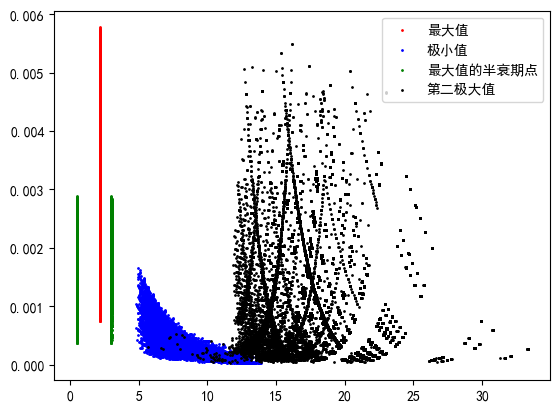
\includegraphics[scale=0.45]{./figs/p3_1.png}
  \caption{所有$A_{plasma}(t)$曲线的五个采样点}
  \label{血浆五点}
\end{figure}

\noindent 可以看到最大值点与两个半衰期点的位置几乎是固定的, 极小值点与第二极大值点几乎都在$30h$前出现. 对于五种采样点, 计算
图\ref{血浆五点}中每种采样点位置的平均值, 将得到的五个平均值作为全局的固定采样点, 它们分别为$(0.49,2.165, 3.005 ,8.22,18.255)$.

对于$A_{urinebps}(t)$与$A_{urinebpsg}(t)$, 由于它们是浓度累计曲线(如图\ref{曲线b}), 难以像血浆BPS含量曲线一样从曲线形状来确定较少的采样点. 由于$A_{urinebps}(t)$是
数值求解的结果, 本质上是一个离散的数组, 故可以对其做一阶差分, 得到某个$A_{urinebps}(t)$的一阶差分曲线如图\ref{尿液差分}所示:
\begin{figure}[H]
  \centering
  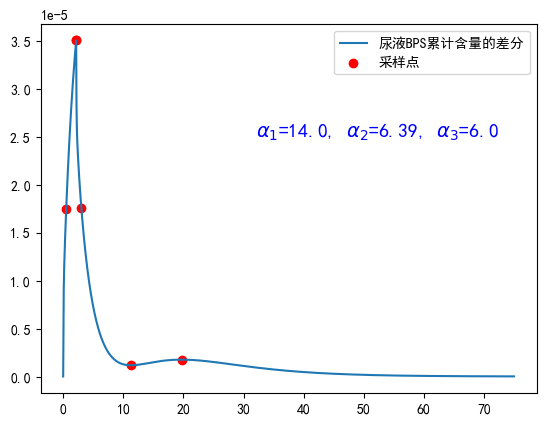
\includegraphics[scale=0.45]{./figs/p4_1.png}
  \caption{$\vec{\alpha}=(14,6.39,6)$时$A_{urinebps}(t)$的一阶差分曲线}
  \label{尿液差分}
\end{figure}

可以看到$A_{urinebps}(t)$的一阶差分曲线有类似于$A_{plasma}(t)$曲线的图像模式, 利用得到血浆曲线的五个全局固定采样点的方式可以得到
两条尿液化学品累计含量曲线的五个全局固定采样点, 它们分别为$(0.505,2.165, 3.04 ,8.265,13.305)$. 图\ref{曲线与采样点5}展示了三条含量曲线的五个固定采样点的位置.

\begin{figure}[H]
  \centering
  \begin{subfigure}{0.45\textwidth}
    \centering
    \resizebox{1\textwidth}{!}{%% Creator: Matplotlib, PGF backend
%%
%% To include the figure in your LaTeX document, write
%%   \input{<filename>.pgf}
%%
%% Make sure the required packages are loaded in your preamble
%%   \usepackage{pgf}
%%
%% Also ensure that all the required font packages are loaded; for instance,
%% the lmodern package is sometimes necessary when using math font.
%%   \usepackage{lmodern}
%%
%% Figures using additional raster images can only be included by \input if
%% they are in the same directory as the main LaTeX file. For loading figures
%% from other directories you can use the `import` package
%%   \usepackage{import}
%%
%% and then include the figures with
%%   \import{<path to file>}{<filename>.pgf}
%%
%% Matplotlib used the following preamble
%%   \def\mathdefault#1{#1}
%%   \everymath=\expandafter{\the\everymath\displaystyle}
%%   
%%   \usepackage{fontspec}
%%   \setmainfont{DejaVuSerif.ttf}[Path=\detokenize{C:/Users/许先生/AppData/Local/Programs/Python/Python310/Lib/site-packages/matplotlib/mpl-data/fonts/ttf/}]
%%   \setsansfont{simhei.ttf}[Path=\detokenize{C:/Windows/Fonts/}]
%%   \setmonofont{DejaVuSansMono.ttf}[Path=\detokenize{C:/Users/许先生/AppData/Local/Programs/Python/Python310/Lib/site-packages/matplotlib/mpl-data/fonts/ttf/}]
%%   \makeatletter\@ifpackageloaded{underscore}{}{\usepackage[strings]{underscore}}\makeatother
%%
\begingroup%
\makeatletter%
\begin{pgfpicture}%
\pgfpathrectangle{\pgfpointorigin}{\pgfqpoint{6.400000in}{4.800000in}}%
\pgfusepath{use as bounding box, clip}%
\begin{pgfscope}%
\pgfsetbuttcap%
\pgfsetmiterjoin%
\definecolor{currentfill}{rgb}{1.000000,1.000000,1.000000}%
\pgfsetfillcolor{currentfill}%
\pgfsetlinewidth{0.000000pt}%
\definecolor{currentstroke}{rgb}{1.000000,1.000000,1.000000}%
\pgfsetstrokecolor{currentstroke}%
\pgfsetdash{}{0pt}%
\pgfpathmoveto{\pgfqpoint{0.000000in}{0.000000in}}%
\pgfpathlineto{\pgfqpoint{6.400000in}{0.000000in}}%
\pgfpathlineto{\pgfqpoint{6.400000in}{4.800000in}}%
\pgfpathlineto{\pgfqpoint{0.000000in}{4.800000in}}%
\pgfpathlineto{\pgfqpoint{0.000000in}{0.000000in}}%
\pgfpathclose%
\pgfusepath{fill}%
\end{pgfscope}%
\begin{pgfscope}%
\pgfsetbuttcap%
\pgfsetmiterjoin%
\definecolor{currentfill}{rgb}{1.000000,1.000000,1.000000}%
\pgfsetfillcolor{currentfill}%
\pgfsetlinewidth{0.000000pt}%
\definecolor{currentstroke}{rgb}{0.000000,0.000000,0.000000}%
\pgfsetstrokecolor{currentstroke}%
\pgfsetstrokeopacity{0.000000}%
\pgfsetdash{}{0pt}%
\pgfpathmoveto{\pgfqpoint{0.800000in}{0.528000in}}%
\pgfpathlineto{\pgfqpoint{5.760000in}{0.528000in}}%
\pgfpathlineto{\pgfqpoint{5.760000in}{4.224000in}}%
\pgfpathlineto{\pgfqpoint{0.800000in}{4.224000in}}%
\pgfpathlineto{\pgfqpoint{0.800000in}{0.528000in}}%
\pgfpathclose%
\pgfusepath{fill}%
\end{pgfscope}%
\begin{pgfscope}%
\pgfpathrectangle{\pgfqpoint{0.800000in}{0.528000in}}{\pgfqpoint{4.960000in}{3.696000in}}%
\pgfusepath{clip}%
\pgfsetbuttcap%
\pgfsetroundjoin%
\definecolor{currentfill}{rgb}{1.000000,0.000000,0.000000}%
\pgfsetfillcolor{currentfill}%
\pgfsetlinewidth{1.003750pt}%
\definecolor{currentstroke}{rgb}{1.000000,0.000000,0.000000}%
\pgfsetstrokecolor{currentstroke}%
\pgfsetdash{}{0pt}%
\pgfsys@defobject{currentmarker}{\pgfqpoint{-0.041667in}{-0.041667in}}{\pgfqpoint{0.041667in}{0.041667in}}{%
\pgfpathmoveto{\pgfqpoint{0.000000in}{-0.041667in}}%
\pgfpathcurveto{\pgfqpoint{0.011050in}{-0.041667in}}{\pgfqpoint{0.021649in}{-0.037276in}}{\pgfqpoint{0.029463in}{-0.029463in}}%
\pgfpathcurveto{\pgfqpoint{0.037276in}{-0.021649in}}{\pgfqpoint{0.041667in}{-0.011050in}}{\pgfqpoint{0.041667in}{0.000000in}}%
\pgfpathcurveto{\pgfqpoint{0.041667in}{0.011050in}}{\pgfqpoint{0.037276in}{0.021649in}}{\pgfqpoint{0.029463in}{0.029463in}}%
\pgfpathcurveto{\pgfqpoint{0.021649in}{0.037276in}}{\pgfqpoint{0.011050in}{0.041667in}}{\pgfqpoint{0.000000in}{0.041667in}}%
\pgfpathcurveto{\pgfqpoint{-0.011050in}{0.041667in}}{\pgfqpoint{-0.021649in}{0.037276in}}{\pgfqpoint{-0.029463in}{0.029463in}}%
\pgfpathcurveto{\pgfqpoint{-0.037276in}{0.021649in}}{\pgfqpoint{-0.041667in}{0.011050in}}{\pgfqpoint{-0.041667in}{0.000000in}}%
\pgfpathcurveto{\pgfqpoint{-0.041667in}{-0.011050in}}{\pgfqpoint{-0.037276in}{-0.021649in}}{\pgfqpoint{-0.029463in}{-0.029463in}}%
\pgfpathcurveto{\pgfqpoint{-0.021649in}{-0.037276in}}{\pgfqpoint{-0.011050in}{-0.041667in}}{\pgfqpoint{0.000000in}{-0.041667in}}%
\pgfpathlineto{\pgfqpoint{0.000000in}{-0.041667in}}%
\pgfpathclose%
\pgfusepath{stroke,fill}%
}%
\begin{pgfscope}%
\pgfsys@transformshift{1.054916in}{2.362722in}%
\pgfsys@useobject{currentmarker}{}%
\end{pgfscope}%
\begin{pgfscope}%
\pgfsys@transformshift{1.155626in}{4.056000in}%
\pgfsys@useobject{currentmarker}{}%
\end{pgfscope}%
\begin{pgfscope}%
\pgfsys@transformshift{1.206131in}{2.374719in}%
\pgfsys@useobject{currentmarker}{}%
\end{pgfscope}%
\begin{pgfscope}%
\pgfsys@transformshift{1.519684in}{0.878660in}%
\pgfsys@useobject{currentmarker}{}%
\end{pgfscope}%
\begin{pgfscope}%
\pgfsys@transformshift{2.123040in}{0.861359in}%
\pgfsys@useobject{currentmarker}{}%
\end{pgfscope}%
\end{pgfscope}%
\begin{pgfscope}%
\pgfsetbuttcap%
\pgfsetroundjoin%
\definecolor{currentfill}{rgb}{0.000000,0.000000,0.000000}%
\pgfsetfillcolor{currentfill}%
\pgfsetlinewidth{0.803000pt}%
\definecolor{currentstroke}{rgb}{0.000000,0.000000,0.000000}%
\pgfsetstrokecolor{currentstroke}%
\pgfsetdash{}{0pt}%
\pgfsys@defobject{currentmarker}{\pgfqpoint{0.000000in}{-0.048611in}}{\pgfqpoint{0.000000in}{0.000000in}}{%
\pgfpathmoveto{\pgfqpoint{0.000000in}{0.000000in}}%
\pgfpathlineto{\pgfqpoint{0.000000in}{-0.048611in}}%
\pgfusepath{stroke,fill}%
}%
\begin{pgfscope}%
\pgfsys@transformshift{1.025455in}{0.528000in}%
\pgfsys@useobject{currentmarker}{}%
\end{pgfscope}%
\end{pgfscope}%
\begin{pgfscope}%
\definecolor{textcolor}{rgb}{0.000000,0.000000,0.000000}%
\pgfsetstrokecolor{textcolor}%
\pgfsetfillcolor{textcolor}%
\pgftext[x=1.025455in,y=0.430778in,,top]{\color{textcolor}{\sffamily\fontsize{10.000000}{12.000000}\selectfont\catcode`\^=\active\def^{\ifmmode\sp\else\^{}\fi}\catcode`\%=\active\def%{\%}0}}%
\end{pgfscope}%
\begin{pgfscope}%
\pgfsetbuttcap%
\pgfsetroundjoin%
\definecolor{currentfill}{rgb}{0.000000,0.000000,0.000000}%
\pgfsetfillcolor{currentfill}%
\pgfsetlinewidth{0.803000pt}%
\definecolor{currentstroke}{rgb}{0.000000,0.000000,0.000000}%
\pgfsetstrokecolor{currentstroke}%
\pgfsetdash{}{0pt}%
\pgfsys@defobject{currentmarker}{\pgfqpoint{0.000000in}{-0.048611in}}{\pgfqpoint{0.000000in}{0.000000in}}{%
\pgfpathmoveto{\pgfqpoint{0.000000in}{0.000000in}}%
\pgfpathlineto{\pgfqpoint{0.000000in}{-0.048611in}}%
\pgfusepath{stroke,fill}%
}%
\begin{pgfscope}%
\pgfsys@transformshift{1.626707in}{0.528000in}%
\pgfsys@useobject{currentmarker}{}%
\end{pgfscope}%
\end{pgfscope}%
\begin{pgfscope}%
\definecolor{textcolor}{rgb}{0.000000,0.000000,0.000000}%
\pgfsetstrokecolor{textcolor}%
\pgfsetfillcolor{textcolor}%
\pgftext[x=1.626707in,y=0.430778in,,top]{\color{textcolor}{\sffamily\fontsize{10.000000}{12.000000}\selectfont\catcode`\^=\active\def^{\ifmmode\sp\else\^{}\fi}\catcode`\%=\active\def%{\%}10}}%
\end{pgfscope}%
\begin{pgfscope}%
\pgfsetbuttcap%
\pgfsetroundjoin%
\definecolor{currentfill}{rgb}{0.000000,0.000000,0.000000}%
\pgfsetfillcolor{currentfill}%
\pgfsetlinewidth{0.803000pt}%
\definecolor{currentstroke}{rgb}{0.000000,0.000000,0.000000}%
\pgfsetstrokecolor{currentstroke}%
\pgfsetdash{}{0pt}%
\pgfsys@defobject{currentmarker}{\pgfqpoint{0.000000in}{-0.048611in}}{\pgfqpoint{0.000000in}{0.000000in}}{%
\pgfpathmoveto{\pgfqpoint{0.000000in}{0.000000in}}%
\pgfpathlineto{\pgfqpoint{0.000000in}{-0.048611in}}%
\pgfusepath{stroke,fill}%
}%
\begin{pgfscope}%
\pgfsys@transformshift{2.227959in}{0.528000in}%
\pgfsys@useobject{currentmarker}{}%
\end{pgfscope}%
\end{pgfscope}%
\begin{pgfscope}%
\definecolor{textcolor}{rgb}{0.000000,0.000000,0.000000}%
\pgfsetstrokecolor{textcolor}%
\pgfsetfillcolor{textcolor}%
\pgftext[x=2.227959in,y=0.430778in,,top]{\color{textcolor}{\sffamily\fontsize{10.000000}{12.000000}\selectfont\catcode`\^=\active\def^{\ifmmode\sp\else\^{}\fi}\catcode`\%=\active\def%{\%}20}}%
\end{pgfscope}%
\begin{pgfscope}%
\pgfsetbuttcap%
\pgfsetroundjoin%
\definecolor{currentfill}{rgb}{0.000000,0.000000,0.000000}%
\pgfsetfillcolor{currentfill}%
\pgfsetlinewidth{0.803000pt}%
\definecolor{currentstroke}{rgb}{0.000000,0.000000,0.000000}%
\pgfsetstrokecolor{currentstroke}%
\pgfsetdash{}{0pt}%
\pgfsys@defobject{currentmarker}{\pgfqpoint{0.000000in}{-0.048611in}}{\pgfqpoint{0.000000in}{0.000000in}}{%
\pgfpathmoveto{\pgfqpoint{0.000000in}{0.000000in}}%
\pgfpathlineto{\pgfqpoint{0.000000in}{-0.048611in}}%
\pgfusepath{stroke,fill}%
}%
\begin{pgfscope}%
\pgfsys@transformshift{2.829211in}{0.528000in}%
\pgfsys@useobject{currentmarker}{}%
\end{pgfscope}%
\end{pgfscope}%
\begin{pgfscope}%
\definecolor{textcolor}{rgb}{0.000000,0.000000,0.000000}%
\pgfsetstrokecolor{textcolor}%
\pgfsetfillcolor{textcolor}%
\pgftext[x=2.829211in,y=0.430778in,,top]{\color{textcolor}{\sffamily\fontsize{10.000000}{12.000000}\selectfont\catcode`\^=\active\def^{\ifmmode\sp\else\^{}\fi}\catcode`\%=\active\def%{\%}30}}%
\end{pgfscope}%
\begin{pgfscope}%
\pgfsetbuttcap%
\pgfsetroundjoin%
\definecolor{currentfill}{rgb}{0.000000,0.000000,0.000000}%
\pgfsetfillcolor{currentfill}%
\pgfsetlinewidth{0.803000pt}%
\definecolor{currentstroke}{rgb}{0.000000,0.000000,0.000000}%
\pgfsetstrokecolor{currentstroke}%
\pgfsetdash{}{0pt}%
\pgfsys@defobject{currentmarker}{\pgfqpoint{0.000000in}{-0.048611in}}{\pgfqpoint{0.000000in}{0.000000in}}{%
\pgfpathmoveto{\pgfqpoint{0.000000in}{0.000000in}}%
\pgfpathlineto{\pgfqpoint{0.000000in}{-0.048611in}}%
\pgfusepath{stroke,fill}%
}%
\begin{pgfscope}%
\pgfsys@transformshift{3.430463in}{0.528000in}%
\pgfsys@useobject{currentmarker}{}%
\end{pgfscope}%
\end{pgfscope}%
\begin{pgfscope}%
\definecolor{textcolor}{rgb}{0.000000,0.000000,0.000000}%
\pgfsetstrokecolor{textcolor}%
\pgfsetfillcolor{textcolor}%
\pgftext[x=3.430463in,y=0.430778in,,top]{\color{textcolor}{\sffamily\fontsize{10.000000}{12.000000}\selectfont\catcode`\^=\active\def^{\ifmmode\sp\else\^{}\fi}\catcode`\%=\active\def%{\%}40}}%
\end{pgfscope}%
\begin{pgfscope}%
\pgfsetbuttcap%
\pgfsetroundjoin%
\definecolor{currentfill}{rgb}{0.000000,0.000000,0.000000}%
\pgfsetfillcolor{currentfill}%
\pgfsetlinewidth{0.803000pt}%
\definecolor{currentstroke}{rgb}{0.000000,0.000000,0.000000}%
\pgfsetstrokecolor{currentstroke}%
\pgfsetdash{}{0pt}%
\pgfsys@defobject{currentmarker}{\pgfqpoint{0.000000in}{-0.048611in}}{\pgfqpoint{0.000000in}{0.000000in}}{%
\pgfpathmoveto{\pgfqpoint{0.000000in}{0.000000in}}%
\pgfpathlineto{\pgfqpoint{0.000000in}{-0.048611in}}%
\pgfusepath{stroke,fill}%
}%
\begin{pgfscope}%
\pgfsys@transformshift{4.031716in}{0.528000in}%
\pgfsys@useobject{currentmarker}{}%
\end{pgfscope}%
\end{pgfscope}%
\begin{pgfscope}%
\definecolor{textcolor}{rgb}{0.000000,0.000000,0.000000}%
\pgfsetstrokecolor{textcolor}%
\pgfsetfillcolor{textcolor}%
\pgftext[x=4.031716in,y=0.430778in,,top]{\color{textcolor}{\sffamily\fontsize{10.000000}{12.000000}\selectfont\catcode`\^=\active\def^{\ifmmode\sp\else\^{}\fi}\catcode`\%=\active\def%{\%}50}}%
\end{pgfscope}%
\begin{pgfscope}%
\pgfsetbuttcap%
\pgfsetroundjoin%
\definecolor{currentfill}{rgb}{0.000000,0.000000,0.000000}%
\pgfsetfillcolor{currentfill}%
\pgfsetlinewidth{0.803000pt}%
\definecolor{currentstroke}{rgb}{0.000000,0.000000,0.000000}%
\pgfsetstrokecolor{currentstroke}%
\pgfsetdash{}{0pt}%
\pgfsys@defobject{currentmarker}{\pgfqpoint{0.000000in}{-0.048611in}}{\pgfqpoint{0.000000in}{0.000000in}}{%
\pgfpathmoveto{\pgfqpoint{0.000000in}{0.000000in}}%
\pgfpathlineto{\pgfqpoint{0.000000in}{-0.048611in}}%
\pgfusepath{stroke,fill}%
}%
\begin{pgfscope}%
\pgfsys@transformshift{4.632968in}{0.528000in}%
\pgfsys@useobject{currentmarker}{}%
\end{pgfscope}%
\end{pgfscope}%
\begin{pgfscope}%
\definecolor{textcolor}{rgb}{0.000000,0.000000,0.000000}%
\pgfsetstrokecolor{textcolor}%
\pgfsetfillcolor{textcolor}%
\pgftext[x=4.632968in,y=0.430778in,,top]{\color{textcolor}{\sffamily\fontsize{10.000000}{12.000000}\selectfont\catcode`\^=\active\def^{\ifmmode\sp\else\^{}\fi}\catcode`\%=\active\def%{\%}60}}%
\end{pgfscope}%
\begin{pgfscope}%
\pgfsetbuttcap%
\pgfsetroundjoin%
\definecolor{currentfill}{rgb}{0.000000,0.000000,0.000000}%
\pgfsetfillcolor{currentfill}%
\pgfsetlinewidth{0.803000pt}%
\definecolor{currentstroke}{rgb}{0.000000,0.000000,0.000000}%
\pgfsetstrokecolor{currentstroke}%
\pgfsetdash{}{0pt}%
\pgfsys@defobject{currentmarker}{\pgfqpoint{0.000000in}{-0.048611in}}{\pgfqpoint{0.000000in}{0.000000in}}{%
\pgfpathmoveto{\pgfqpoint{0.000000in}{0.000000in}}%
\pgfpathlineto{\pgfqpoint{0.000000in}{-0.048611in}}%
\pgfusepath{stroke,fill}%
}%
\begin{pgfscope}%
\pgfsys@transformshift{5.234220in}{0.528000in}%
\pgfsys@useobject{currentmarker}{}%
\end{pgfscope}%
\end{pgfscope}%
\begin{pgfscope}%
\definecolor{textcolor}{rgb}{0.000000,0.000000,0.000000}%
\pgfsetstrokecolor{textcolor}%
\pgfsetfillcolor{textcolor}%
\pgftext[x=5.234220in,y=0.430778in,,top]{\color{textcolor}{\sffamily\fontsize{10.000000}{12.000000}\selectfont\catcode`\^=\active\def^{\ifmmode\sp\else\^{}\fi}\catcode`\%=\active\def%{\%}70}}%
\end{pgfscope}%
\begin{pgfscope}%
\pgfsetbuttcap%
\pgfsetroundjoin%
\definecolor{currentfill}{rgb}{0.000000,0.000000,0.000000}%
\pgfsetfillcolor{currentfill}%
\pgfsetlinewidth{0.803000pt}%
\definecolor{currentstroke}{rgb}{0.000000,0.000000,0.000000}%
\pgfsetstrokecolor{currentstroke}%
\pgfsetdash{}{0pt}%
\pgfsys@defobject{currentmarker}{\pgfqpoint{-0.048611in}{0.000000in}}{\pgfqpoint{-0.000000in}{0.000000in}}{%
\pgfpathmoveto{\pgfqpoint{-0.000000in}{0.000000in}}%
\pgfpathlineto{\pgfqpoint{-0.048611in}{0.000000in}}%
\pgfusepath{stroke,fill}%
}%
\begin{pgfscope}%
\pgfsys@transformshift{0.800000in}{0.696000in}%
\pgfsys@useobject{currentmarker}{}%
\end{pgfscope}%
\end{pgfscope}%
\begin{pgfscope}%
\definecolor{textcolor}{rgb}{0.000000,0.000000,0.000000}%
\pgfsetstrokecolor{textcolor}%
\pgfsetfillcolor{textcolor}%
\pgftext[x=0.286111in, y=0.648257in, left, base]{\color{textcolor}{\sffamily\fontsize{10.000000}{12.000000}\selectfont\catcode`\^=\active\def^{\ifmmode\sp\else\^{}\fi}\catcode`\%=\active\def%{\%}0.0000}}%
\end{pgfscope}%
\begin{pgfscope}%
\pgfsetbuttcap%
\pgfsetroundjoin%
\definecolor{currentfill}{rgb}{0.000000,0.000000,0.000000}%
\pgfsetfillcolor{currentfill}%
\pgfsetlinewidth{0.803000pt}%
\definecolor{currentstroke}{rgb}{0.000000,0.000000,0.000000}%
\pgfsetstrokecolor{currentstroke}%
\pgfsetdash{}{0pt}%
\pgfsys@defobject{currentmarker}{\pgfqpoint{-0.048611in}{0.000000in}}{\pgfqpoint{-0.000000in}{0.000000in}}{%
\pgfpathmoveto{\pgfqpoint{-0.000000in}{0.000000in}}%
\pgfpathlineto{\pgfqpoint{-0.048611in}{0.000000in}}%
\pgfusepath{stroke,fill}%
}%
\begin{pgfscope}%
\pgfsys@transformshift{0.800000in}{1.212396in}%
\pgfsys@useobject{currentmarker}{}%
\end{pgfscope}%
\end{pgfscope}%
\begin{pgfscope}%
\definecolor{textcolor}{rgb}{0.000000,0.000000,0.000000}%
\pgfsetstrokecolor{textcolor}%
\pgfsetfillcolor{textcolor}%
\pgftext[x=0.286111in, y=1.164653in, left, base]{\color{textcolor}{\sffamily\fontsize{10.000000}{12.000000}\selectfont\catcode`\^=\active\def^{\ifmmode\sp\else\^{}\fi}\catcode`\%=\active\def%{\%}0.0005}}%
\end{pgfscope}%
\begin{pgfscope}%
\pgfsetbuttcap%
\pgfsetroundjoin%
\definecolor{currentfill}{rgb}{0.000000,0.000000,0.000000}%
\pgfsetfillcolor{currentfill}%
\pgfsetlinewidth{0.803000pt}%
\definecolor{currentstroke}{rgb}{0.000000,0.000000,0.000000}%
\pgfsetstrokecolor{currentstroke}%
\pgfsetdash{}{0pt}%
\pgfsys@defobject{currentmarker}{\pgfqpoint{-0.048611in}{0.000000in}}{\pgfqpoint{-0.000000in}{0.000000in}}{%
\pgfpathmoveto{\pgfqpoint{-0.000000in}{0.000000in}}%
\pgfpathlineto{\pgfqpoint{-0.048611in}{0.000000in}}%
\pgfusepath{stroke,fill}%
}%
\begin{pgfscope}%
\pgfsys@transformshift{0.800000in}{1.728792in}%
\pgfsys@useobject{currentmarker}{}%
\end{pgfscope}%
\end{pgfscope}%
\begin{pgfscope}%
\definecolor{textcolor}{rgb}{0.000000,0.000000,0.000000}%
\pgfsetstrokecolor{textcolor}%
\pgfsetfillcolor{textcolor}%
\pgftext[x=0.286111in, y=1.681049in, left, base]{\color{textcolor}{\sffamily\fontsize{10.000000}{12.000000}\selectfont\catcode`\^=\active\def^{\ifmmode\sp\else\^{}\fi}\catcode`\%=\active\def%{\%}0.0010}}%
\end{pgfscope}%
\begin{pgfscope}%
\pgfsetbuttcap%
\pgfsetroundjoin%
\definecolor{currentfill}{rgb}{0.000000,0.000000,0.000000}%
\pgfsetfillcolor{currentfill}%
\pgfsetlinewidth{0.803000pt}%
\definecolor{currentstroke}{rgb}{0.000000,0.000000,0.000000}%
\pgfsetstrokecolor{currentstroke}%
\pgfsetdash{}{0pt}%
\pgfsys@defobject{currentmarker}{\pgfqpoint{-0.048611in}{0.000000in}}{\pgfqpoint{-0.000000in}{0.000000in}}{%
\pgfpathmoveto{\pgfqpoint{-0.000000in}{0.000000in}}%
\pgfpathlineto{\pgfqpoint{-0.048611in}{0.000000in}}%
\pgfusepath{stroke,fill}%
}%
\begin{pgfscope}%
\pgfsys@transformshift{0.800000in}{2.245188in}%
\pgfsys@useobject{currentmarker}{}%
\end{pgfscope}%
\end{pgfscope}%
\begin{pgfscope}%
\definecolor{textcolor}{rgb}{0.000000,0.000000,0.000000}%
\pgfsetstrokecolor{textcolor}%
\pgfsetfillcolor{textcolor}%
\pgftext[x=0.286111in, y=2.197445in, left, base]{\color{textcolor}{\sffamily\fontsize{10.000000}{12.000000}\selectfont\catcode`\^=\active\def^{\ifmmode\sp\else\^{}\fi}\catcode`\%=\active\def%{\%}0.0015}}%
\end{pgfscope}%
\begin{pgfscope}%
\pgfsetbuttcap%
\pgfsetroundjoin%
\definecolor{currentfill}{rgb}{0.000000,0.000000,0.000000}%
\pgfsetfillcolor{currentfill}%
\pgfsetlinewidth{0.803000pt}%
\definecolor{currentstroke}{rgb}{0.000000,0.000000,0.000000}%
\pgfsetstrokecolor{currentstroke}%
\pgfsetdash{}{0pt}%
\pgfsys@defobject{currentmarker}{\pgfqpoint{-0.048611in}{0.000000in}}{\pgfqpoint{-0.000000in}{0.000000in}}{%
\pgfpathmoveto{\pgfqpoint{-0.000000in}{0.000000in}}%
\pgfpathlineto{\pgfqpoint{-0.048611in}{0.000000in}}%
\pgfusepath{stroke,fill}%
}%
\begin{pgfscope}%
\pgfsys@transformshift{0.800000in}{2.761584in}%
\pgfsys@useobject{currentmarker}{}%
\end{pgfscope}%
\end{pgfscope}%
\begin{pgfscope}%
\definecolor{textcolor}{rgb}{0.000000,0.000000,0.000000}%
\pgfsetstrokecolor{textcolor}%
\pgfsetfillcolor{textcolor}%
\pgftext[x=0.286111in, y=2.713841in, left, base]{\color{textcolor}{\sffamily\fontsize{10.000000}{12.000000}\selectfont\catcode`\^=\active\def^{\ifmmode\sp\else\^{}\fi}\catcode`\%=\active\def%{\%}0.0020}}%
\end{pgfscope}%
\begin{pgfscope}%
\pgfsetbuttcap%
\pgfsetroundjoin%
\definecolor{currentfill}{rgb}{0.000000,0.000000,0.000000}%
\pgfsetfillcolor{currentfill}%
\pgfsetlinewidth{0.803000pt}%
\definecolor{currentstroke}{rgb}{0.000000,0.000000,0.000000}%
\pgfsetstrokecolor{currentstroke}%
\pgfsetdash{}{0pt}%
\pgfsys@defobject{currentmarker}{\pgfqpoint{-0.048611in}{0.000000in}}{\pgfqpoint{-0.000000in}{0.000000in}}{%
\pgfpathmoveto{\pgfqpoint{-0.000000in}{0.000000in}}%
\pgfpathlineto{\pgfqpoint{-0.048611in}{0.000000in}}%
\pgfusepath{stroke,fill}%
}%
\begin{pgfscope}%
\pgfsys@transformshift{0.800000in}{3.277981in}%
\pgfsys@useobject{currentmarker}{}%
\end{pgfscope}%
\end{pgfscope}%
\begin{pgfscope}%
\definecolor{textcolor}{rgb}{0.000000,0.000000,0.000000}%
\pgfsetstrokecolor{textcolor}%
\pgfsetfillcolor{textcolor}%
\pgftext[x=0.286111in, y=3.230238in, left, base]{\color{textcolor}{\sffamily\fontsize{10.000000}{12.000000}\selectfont\catcode`\^=\active\def^{\ifmmode\sp\else\^{}\fi}\catcode`\%=\active\def%{\%}0.0025}}%
\end{pgfscope}%
\begin{pgfscope}%
\pgfsetbuttcap%
\pgfsetroundjoin%
\definecolor{currentfill}{rgb}{0.000000,0.000000,0.000000}%
\pgfsetfillcolor{currentfill}%
\pgfsetlinewidth{0.803000pt}%
\definecolor{currentstroke}{rgb}{0.000000,0.000000,0.000000}%
\pgfsetstrokecolor{currentstroke}%
\pgfsetdash{}{0pt}%
\pgfsys@defobject{currentmarker}{\pgfqpoint{-0.048611in}{0.000000in}}{\pgfqpoint{-0.000000in}{0.000000in}}{%
\pgfpathmoveto{\pgfqpoint{-0.000000in}{0.000000in}}%
\pgfpathlineto{\pgfqpoint{-0.048611in}{0.000000in}}%
\pgfusepath{stroke,fill}%
}%
\begin{pgfscope}%
\pgfsys@transformshift{0.800000in}{3.794377in}%
\pgfsys@useobject{currentmarker}{}%
\end{pgfscope}%
\end{pgfscope}%
\begin{pgfscope}%
\definecolor{textcolor}{rgb}{0.000000,0.000000,0.000000}%
\pgfsetstrokecolor{textcolor}%
\pgfsetfillcolor{textcolor}%
\pgftext[x=0.286111in, y=3.746634in, left, base]{\color{textcolor}{\sffamily\fontsize{10.000000}{12.000000}\selectfont\catcode`\^=\active\def^{\ifmmode\sp\else\^{}\fi}\catcode`\%=\active\def%{\%}0.0030}}%
\end{pgfscope}%
\begin{pgfscope}%
\pgfpathrectangle{\pgfqpoint{0.800000in}{0.528000in}}{\pgfqpoint{4.960000in}{3.696000in}}%
\pgfusepath{clip}%
\pgfsetrectcap%
\pgfsetroundjoin%
\pgfsetlinewidth{1.505625pt}%
\definecolor{currentstroke}{rgb}{0.121569,0.466667,0.705882}%
\pgfsetstrokecolor{currentstroke}%
\pgfsetdash{}{0pt}%
\pgfpathmoveto{\pgfqpoint{1.025455in}{0.696000in}}%
\pgfpathlineto{\pgfqpoint{1.026056in}{0.762430in}}%
\pgfpathlineto{\pgfqpoint{1.029363in}{1.438319in}}%
\pgfpathlineto{\pgfqpoint{1.032970in}{1.685865in}}%
\pgfpathlineto{\pgfqpoint{1.038381in}{1.898418in}}%
\pgfpathlineto{\pgfqpoint{1.048302in}{2.190817in}}%
\pgfpathlineto{\pgfqpoint{1.062732in}{2.550505in}}%
\pgfpathlineto{\pgfqpoint{1.078665in}{2.893246in}}%
\pgfpathlineto{\pgfqpoint{1.095500in}{3.209049in}}%
\pgfpathlineto{\pgfqpoint{1.112937in}{3.495189in}}%
\pgfpathlineto{\pgfqpoint{1.130674in}{3.749981in}}%
\pgfpathlineto{\pgfqpoint{1.148411in}{3.973226in}}%
\pgfpathlineto{\pgfqpoint{1.155626in}{4.056000in}}%
\pgfpathlineto{\pgfqpoint{1.161037in}{3.223808in}}%
\pgfpathlineto{\pgfqpoint{1.164945in}{3.072237in}}%
\pgfpathlineto{\pgfqpoint{1.170958in}{2.928909in}}%
\pgfpathlineto{\pgfqpoint{1.181479in}{2.735275in}}%
\pgfpathlineto{\pgfqpoint{1.195308in}{2.521517in}}%
\pgfpathlineto{\pgfqpoint{1.210941in}{2.314014in}}%
\pgfpathlineto{\pgfqpoint{1.227776in}{2.119944in}}%
\pgfpathlineto{\pgfqpoint{1.244912in}{1.947537in}}%
\pgfpathlineto{\pgfqpoint{1.262348in}{1.794109in}}%
\pgfpathlineto{\pgfqpoint{1.279784in}{1.659865in}}%
\pgfpathlineto{\pgfqpoint{1.297221in}{1.542338in}}%
\pgfpathlineto{\pgfqpoint{1.314957in}{1.437787in}}%
\pgfpathlineto{\pgfqpoint{1.332394in}{1.347922in}}%
\pgfpathlineto{\pgfqpoint{1.349830in}{1.269301in}}%
\pgfpathlineto{\pgfqpoint{1.367266in}{1.200569in}}%
\pgfpathlineto{\pgfqpoint{1.384703in}{1.140552in}}%
\pgfpathlineto{\pgfqpoint{1.402139in}{1.088215in}}%
\pgfpathlineto{\pgfqpoint{1.419575in}{1.042676in}}%
\pgfpathlineto{\pgfqpoint{1.437312in}{1.002509in}}%
\pgfpathlineto{\pgfqpoint{1.454749in}{0.968381in}}%
\pgfpathlineto{\pgfqpoint{1.472185in}{0.938966in}}%
\pgfpathlineto{\pgfqpoint{1.489922in}{0.913318in}}%
\pgfpathlineto{\pgfqpoint{1.507659in}{0.891498in}}%
\pgfpathlineto{\pgfqpoint{1.525696in}{0.872785in}}%
\pgfpathlineto{\pgfqpoint{1.544035in}{0.856940in}}%
\pgfpathlineto{\pgfqpoint{1.562974in}{0.843533in}}%
\pgfpathlineto{\pgfqpoint{1.582214in}{0.832613in}}%
\pgfpathlineto{\pgfqpoint{1.602657in}{0.823615in}}%
\pgfpathlineto{\pgfqpoint{1.624001in}{0.816686in}}%
\pgfpathlineto{\pgfqpoint{1.646849in}{0.811651in}}%
\pgfpathlineto{\pgfqpoint{1.671500in}{0.808530in}}%
\pgfpathlineto{\pgfqpoint{1.698857in}{0.807358in}}%
\pgfpathlineto{\pgfqpoint{1.729822in}{0.808312in}}%
\pgfpathlineto{\pgfqpoint{1.766498in}{0.811744in}}%
\pgfpathlineto{\pgfqpoint{1.813696in}{0.818523in}}%
\pgfpathlineto{\pgfqpoint{1.903283in}{0.834202in}}%
\pgfpathlineto{\pgfqpoint{1.986556in}{0.847690in}}%
\pgfpathlineto{\pgfqpoint{2.047583in}{0.855297in}}%
\pgfpathlineto{\pgfqpoint{2.103800in}{0.860184in}}%
\pgfpathlineto{\pgfqpoint{2.161220in}{0.862954in}}%
\pgfpathlineto{\pgfqpoint{2.219241in}{0.863578in}}%
\pgfpathlineto{\pgfqpoint{2.280869in}{0.862074in}}%
\pgfpathlineto{\pgfqpoint{2.349713in}{0.858143in}}%
\pgfpathlineto{\pgfqpoint{2.428176in}{0.851366in}}%
\pgfpathlineto{\pgfqpoint{2.523775in}{0.840778in}}%
\pgfpathlineto{\pgfqpoint{2.663566in}{0.822817in}}%
\pgfpathlineto{\pgfqpoint{2.955474in}{0.784990in}}%
\pgfpathlineto{\pgfqpoint{3.097069in}{0.769068in}}%
\pgfpathlineto{\pgfqpoint{3.238363in}{0.755364in}}%
\pgfpathlineto{\pgfqpoint{3.382964in}{0.743589in}}%
\pgfpathlineto{\pgfqpoint{3.537186in}{0.733318in}}%
\pgfpathlineto{\pgfqpoint{3.702831in}{0.724568in}}%
\pgfpathlineto{\pgfqpoint{3.887114in}{0.717106in}}%
\pgfpathlineto{\pgfqpoint{4.097853in}{0.710856in}}%
\pgfpathlineto{\pgfqpoint{4.347072in}{0.705763in}}%
\pgfpathlineto{\pgfqpoint{4.655214in}{0.701783in}}%
\pgfpathlineto{\pgfqpoint{5.061961in}{0.698886in}}%
\pgfpathlineto{\pgfqpoint{5.534545in}{0.697283in}}%
\pgfpathlineto{\pgfqpoint{5.534545in}{0.697283in}}%
\pgfusepath{stroke}%
\end{pgfscope}%
\begin{pgfscope}%
\pgfsetrectcap%
\pgfsetmiterjoin%
\pgfsetlinewidth{0.803000pt}%
\definecolor{currentstroke}{rgb}{0.000000,0.000000,0.000000}%
\pgfsetstrokecolor{currentstroke}%
\pgfsetdash{}{0pt}%
\pgfpathmoveto{\pgfqpoint{0.800000in}{0.528000in}}%
\pgfpathlineto{\pgfqpoint{0.800000in}{4.224000in}}%
\pgfusepath{stroke}%
\end{pgfscope}%
\begin{pgfscope}%
\pgfsetrectcap%
\pgfsetmiterjoin%
\pgfsetlinewidth{0.803000pt}%
\definecolor{currentstroke}{rgb}{0.000000,0.000000,0.000000}%
\pgfsetstrokecolor{currentstroke}%
\pgfsetdash{}{0pt}%
\pgfpathmoveto{\pgfqpoint{5.760000in}{0.528000in}}%
\pgfpathlineto{\pgfqpoint{5.760000in}{4.224000in}}%
\pgfusepath{stroke}%
\end{pgfscope}%
\begin{pgfscope}%
\pgfsetrectcap%
\pgfsetmiterjoin%
\pgfsetlinewidth{0.803000pt}%
\definecolor{currentstroke}{rgb}{0.000000,0.000000,0.000000}%
\pgfsetstrokecolor{currentstroke}%
\pgfsetdash{}{0pt}%
\pgfpathmoveto{\pgfqpoint{0.800000in}{0.528000in}}%
\pgfpathlineto{\pgfqpoint{5.760000in}{0.528000in}}%
\pgfusepath{stroke}%
\end{pgfscope}%
\begin{pgfscope}%
\pgfsetrectcap%
\pgfsetmiterjoin%
\pgfsetlinewidth{0.803000pt}%
\definecolor{currentstroke}{rgb}{0.000000,0.000000,0.000000}%
\pgfsetstrokecolor{currentstroke}%
\pgfsetdash{}{0pt}%
\pgfpathmoveto{\pgfqpoint{0.800000in}{4.224000in}}%
\pgfpathlineto{\pgfqpoint{5.760000in}{4.224000in}}%
\pgfusepath{stroke}%
\end{pgfscope}%
\begin{pgfscope}%
\definecolor{textcolor}{rgb}{0.000000,0.000000,1.000000}%
\pgfsetstrokecolor{textcolor}%
\pgfsetfillcolor{textcolor}%
\pgftext[x=2.560000in,y=2.880000in,left,base]{\color{textcolor}{\sffamily\fontsize{14.000000}{16.800000}\bfseries\selectfont\catcode`\^=\active\def^{\ifmmode\sp\else\^{}\fi}\catcode`\%=\active\def%{\%}$\alpha_1$=14.0, $\alpha_2$=6.39, $\alpha_3$=6.0}}%
\end{pgfscope}%
\begin{pgfscope}%
\pgfsetbuttcap%
\pgfsetmiterjoin%
\definecolor{currentfill}{rgb}{1.000000,1.000000,1.000000}%
\pgfsetfillcolor{currentfill}%
\pgfsetfillopacity{0.800000}%
\pgfsetlinewidth{1.003750pt}%
\definecolor{currentstroke}{rgb}{0.800000,0.800000,0.800000}%
\pgfsetstrokecolor{currentstroke}%
\pgfsetstrokeopacity{0.800000}%
\pgfsetdash{}{0pt}%
\pgfpathmoveto{\pgfqpoint{4.454444in}{3.719009in}}%
\pgfpathlineto{\pgfqpoint{5.662778in}{3.719009in}}%
\pgfpathquadraticcurveto{\pgfqpoint{5.690556in}{3.719009in}}{\pgfqpoint{5.690556in}{3.746787in}}%
\pgfpathlineto{\pgfqpoint{5.690556in}{4.126778in}}%
\pgfpathquadraticcurveto{\pgfqpoint{5.690556in}{4.154556in}}{\pgfqpoint{5.662778in}{4.154556in}}%
\pgfpathlineto{\pgfqpoint{4.454444in}{4.154556in}}%
\pgfpathquadraticcurveto{\pgfqpoint{4.426667in}{4.154556in}}{\pgfqpoint{4.426667in}{4.126778in}}%
\pgfpathlineto{\pgfqpoint{4.426667in}{3.746787in}}%
\pgfpathquadraticcurveto{\pgfqpoint{4.426667in}{3.719009in}}{\pgfqpoint{4.454444in}{3.719009in}}%
\pgfpathlineto{\pgfqpoint{4.454444in}{3.719009in}}%
\pgfpathclose%
\pgfusepath{stroke,fill}%
\end{pgfscope}%
\begin{pgfscope}%
\pgfsetrectcap%
\pgfsetroundjoin%
\pgfsetlinewidth{1.505625pt}%
\definecolor{currentstroke}{rgb}{0.121569,0.466667,0.705882}%
\pgfsetstrokecolor{currentstroke}%
\pgfsetdash{}{0pt}%
\pgfpathmoveto{\pgfqpoint{4.482222in}{4.036934in}}%
\pgfpathlineto{\pgfqpoint{4.621111in}{4.036934in}}%
\pgfpathlineto{\pgfqpoint{4.760000in}{4.036934in}}%
\pgfusepath{stroke}%
\end{pgfscope}%
\begin{pgfscope}%
\definecolor{textcolor}{rgb}{0.000000,0.000000,0.000000}%
\pgfsetstrokecolor{textcolor}%
\pgfsetfillcolor{textcolor}%
\pgftext[x=4.871111in,y=3.988323in,left,base]{\color{textcolor}{\sffamily\fontsize{10.000000}{12.000000}\selectfont\catcode`\^=\active\def^{\ifmmode\sp\else\^{}\fi}\catcode`\%=\active\def%{\%}血浆BPS含量}}%
\end{pgfscope}%
\begin{pgfscope}%
\pgfsetbuttcap%
\pgfsetroundjoin%
\definecolor{currentfill}{rgb}{1.000000,0.000000,0.000000}%
\pgfsetfillcolor{currentfill}%
\pgfsetlinewidth{1.003750pt}%
\definecolor{currentstroke}{rgb}{1.000000,0.000000,0.000000}%
\pgfsetstrokecolor{currentstroke}%
\pgfsetdash{}{0pt}%
\pgfsys@defobject{currentmarker}{\pgfqpoint{-0.041667in}{-0.041667in}}{\pgfqpoint{0.041667in}{0.041667in}}{%
\pgfpathmoveto{\pgfqpoint{0.000000in}{-0.041667in}}%
\pgfpathcurveto{\pgfqpoint{0.011050in}{-0.041667in}}{\pgfqpoint{0.021649in}{-0.037276in}}{\pgfqpoint{0.029463in}{-0.029463in}}%
\pgfpathcurveto{\pgfqpoint{0.037276in}{-0.021649in}}{\pgfqpoint{0.041667in}{-0.011050in}}{\pgfqpoint{0.041667in}{0.000000in}}%
\pgfpathcurveto{\pgfqpoint{0.041667in}{0.011050in}}{\pgfqpoint{0.037276in}{0.021649in}}{\pgfqpoint{0.029463in}{0.029463in}}%
\pgfpathcurveto{\pgfqpoint{0.021649in}{0.037276in}}{\pgfqpoint{0.011050in}{0.041667in}}{\pgfqpoint{0.000000in}{0.041667in}}%
\pgfpathcurveto{\pgfqpoint{-0.011050in}{0.041667in}}{\pgfqpoint{-0.021649in}{0.037276in}}{\pgfqpoint{-0.029463in}{0.029463in}}%
\pgfpathcurveto{\pgfqpoint{-0.037276in}{0.021649in}}{\pgfqpoint{-0.041667in}{0.011050in}}{\pgfqpoint{-0.041667in}{0.000000in}}%
\pgfpathcurveto{\pgfqpoint{-0.041667in}{-0.011050in}}{\pgfqpoint{-0.037276in}{-0.021649in}}{\pgfqpoint{-0.029463in}{-0.029463in}}%
\pgfpathcurveto{\pgfqpoint{-0.021649in}{-0.037276in}}{\pgfqpoint{-0.011050in}{-0.041667in}}{\pgfqpoint{0.000000in}{-0.041667in}}%
\pgfpathlineto{\pgfqpoint{0.000000in}{-0.041667in}}%
\pgfpathclose%
\pgfusepath{stroke,fill}%
}%
\begin{pgfscope}%
\pgfsys@transformshift{4.621111in}{3.828384in}%
\pgfsys@useobject{currentmarker}{}%
\end{pgfscope}%
\end{pgfscope}%
\begin{pgfscope}%
\definecolor{textcolor}{rgb}{0.000000,0.000000,0.000000}%
\pgfsetstrokecolor{textcolor}%
\pgfsetfillcolor{textcolor}%
\pgftext[x=4.871111in,y=3.791925in,left,base]{\color{textcolor}{\sffamily\fontsize{10.000000}{12.000000}\selectfont\catcode`\^=\active\def^{\ifmmode\sp\else\^{}\fi}\catcode`\%=\active\def%{\%}采样点}}%
\end{pgfscope}%
\end{pgfpicture}%
\makeatother%
\endgroup%
}
    \caption{$A_{plasma}(t)$与5点采样点}
    \label{曲线与采样点5a}
  \end{subfigure}
  \begin{subfigure}{0.45\textwidth}
    \centering
    \resizebox{1\textwidth}{!}{%% Creator: Matplotlib, PGF backend
%%
%% To include the figure in your LaTeX document, write
%%   \input{<filename>.pgf}
%%
%% Make sure the required packages are loaded in your preamble
%%   \usepackage{pgf}
%%
%% Also ensure that all the required font packages are loaded; for instance,
%% the lmodern package is sometimes necessary when using math font.
%%   \usepackage{lmodern}
%%
%% Figures using additional raster images can only be included by \input if
%% they are in the same directory as the main LaTeX file. For loading figures
%% from other directories you can use the `import` package
%%   \usepackage{import}
%%
%% and then include the figures with
%%   \import{<path to file>}{<filename>.pgf}
%%
%% Matplotlib used the following preamble
%%   \def\mathdefault#1{#1}
%%   \everymath=\expandafter{\the\everymath\displaystyle}
%%   
%%   \usepackage{fontspec}
%%   \setmainfont{DejaVuSerif.ttf}[Path=\detokenize{C:/Users/许先生/AppData/Local/Programs/Python/Python310/Lib/site-packages/matplotlib/mpl-data/fonts/ttf/}]
%%   \setsansfont{simhei.ttf}[Path=\detokenize{C:/Windows/Fonts/}]
%%   \setmonofont{DejaVuSansMono.ttf}[Path=\detokenize{C:/Users/许先生/AppData/Local/Programs/Python/Python310/Lib/site-packages/matplotlib/mpl-data/fonts/ttf/}]
%%   \makeatletter\@ifpackageloaded{underscore}{}{\usepackage[strings]{underscore}}\makeatother
%%
\begingroup%
\makeatletter%
\begin{pgfpicture}%
\pgfpathrectangle{\pgfpointorigin}{\pgfqpoint{6.400000in}{4.800000in}}%
\pgfusepath{use as bounding box, clip}%
\begin{pgfscope}%
\pgfsetbuttcap%
\pgfsetmiterjoin%
\definecolor{currentfill}{rgb}{1.000000,1.000000,1.000000}%
\pgfsetfillcolor{currentfill}%
\pgfsetlinewidth{0.000000pt}%
\definecolor{currentstroke}{rgb}{1.000000,1.000000,1.000000}%
\pgfsetstrokecolor{currentstroke}%
\pgfsetdash{}{0pt}%
\pgfpathmoveto{\pgfqpoint{0.000000in}{0.000000in}}%
\pgfpathlineto{\pgfqpoint{6.400000in}{0.000000in}}%
\pgfpathlineto{\pgfqpoint{6.400000in}{4.800000in}}%
\pgfpathlineto{\pgfqpoint{0.000000in}{4.800000in}}%
\pgfpathlineto{\pgfqpoint{0.000000in}{0.000000in}}%
\pgfpathclose%
\pgfusepath{fill}%
\end{pgfscope}%
\begin{pgfscope}%
\pgfsetbuttcap%
\pgfsetmiterjoin%
\definecolor{currentfill}{rgb}{1.000000,1.000000,1.000000}%
\pgfsetfillcolor{currentfill}%
\pgfsetlinewidth{0.000000pt}%
\definecolor{currentstroke}{rgb}{0.000000,0.000000,0.000000}%
\pgfsetstrokecolor{currentstroke}%
\pgfsetstrokeopacity{0.000000}%
\pgfsetdash{}{0pt}%
\pgfpathmoveto{\pgfqpoint{0.800000in}{0.528000in}}%
\pgfpathlineto{\pgfqpoint{5.760000in}{0.528000in}}%
\pgfpathlineto{\pgfqpoint{5.760000in}{4.224000in}}%
\pgfpathlineto{\pgfqpoint{0.800000in}{4.224000in}}%
\pgfpathlineto{\pgfqpoint{0.800000in}{0.528000in}}%
\pgfpathclose%
\pgfusepath{fill}%
\end{pgfscope}%
\begin{pgfscope}%
\pgfpathrectangle{\pgfqpoint{0.800000in}{0.528000in}}{\pgfqpoint{4.960000in}{3.696000in}}%
\pgfusepath{clip}%
\pgfsetbuttcap%
\pgfsetroundjoin%
\definecolor{currentfill}{rgb}{1.000000,0.000000,0.000000}%
\pgfsetfillcolor{currentfill}%
\pgfsetlinewidth{1.003750pt}%
\definecolor{currentstroke}{rgb}{1.000000,0.000000,0.000000}%
\pgfsetstrokecolor{currentstroke}%
\pgfsetdash{}{0pt}%
\pgfsys@defobject{currentmarker}{\pgfqpoint{-0.041667in}{-0.041667in}}{\pgfqpoint{0.041667in}{0.041667in}}{%
\pgfpathmoveto{\pgfqpoint{0.000000in}{-0.041667in}}%
\pgfpathcurveto{\pgfqpoint{0.011050in}{-0.041667in}}{\pgfqpoint{0.021649in}{-0.037276in}}{\pgfqpoint{0.029463in}{-0.029463in}}%
\pgfpathcurveto{\pgfqpoint{0.037276in}{-0.021649in}}{\pgfqpoint{0.041667in}{-0.011050in}}{\pgfqpoint{0.041667in}{0.000000in}}%
\pgfpathcurveto{\pgfqpoint{0.041667in}{0.011050in}}{\pgfqpoint{0.037276in}{0.021649in}}{\pgfqpoint{0.029463in}{0.029463in}}%
\pgfpathcurveto{\pgfqpoint{0.021649in}{0.037276in}}{\pgfqpoint{0.011050in}{0.041667in}}{\pgfqpoint{0.000000in}{0.041667in}}%
\pgfpathcurveto{\pgfqpoint{-0.011050in}{0.041667in}}{\pgfqpoint{-0.021649in}{0.037276in}}{\pgfqpoint{-0.029463in}{0.029463in}}%
\pgfpathcurveto{\pgfqpoint{-0.037276in}{0.021649in}}{\pgfqpoint{-0.041667in}{0.011050in}}{\pgfqpoint{-0.041667in}{0.000000in}}%
\pgfpathcurveto{\pgfqpoint{-0.041667in}{-0.011050in}}{\pgfqpoint{-0.037276in}{-0.021649in}}{\pgfqpoint{-0.029463in}{-0.029463in}}%
\pgfpathcurveto{\pgfqpoint{-0.021649in}{-0.037276in}}{\pgfqpoint{-0.011050in}{-0.041667in}}{\pgfqpoint{0.000000in}{-0.041667in}}%
\pgfpathlineto{\pgfqpoint{0.000000in}{-0.041667in}}%
\pgfpathclose%
\pgfusepath{stroke,fill}%
}%
\begin{pgfscope}%
\pgfsys@transformshift{1.055818in}{0.745683in}%
\pgfsys@useobject{currentmarker}{}%
\end{pgfscope}%
\begin{pgfscope}%
\pgfsys@transformshift{1.155626in}{1.116182in}%
\pgfsys@useobject{currentmarker}{}%
\end{pgfscope}%
\begin{pgfscope}%
\pgfsys@transformshift{1.208235in}{1.274593in}%
\pgfsys@useobject{currentmarker}{}%
\end{pgfscope}%
\begin{pgfscope}%
\pgfsys@transformshift{1.522389in}{1.565427in}%
\pgfsys@useobject{currentmarker}{}%
\end{pgfscope}%
\begin{pgfscope}%
\pgfsys@transformshift{2.126047in}{1.683397in}%
\pgfsys@useobject{currentmarker}{}%
\end{pgfscope}%
\end{pgfscope}%
\begin{pgfscope}%
\pgfpathrectangle{\pgfqpoint{0.800000in}{0.528000in}}{\pgfqpoint{4.960000in}{3.696000in}}%
\pgfusepath{clip}%
\pgfsetbuttcap%
\pgfsetroundjoin%
\definecolor{currentfill}{rgb}{0.000000,0.501961,0.000000}%
\pgfsetfillcolor{currentfill}%
\pgfsetlinewidth{1.003750pt}%
\definecolor{currentstroke}{rgb}{0.000000,0.501961,0.000000}%
\pgfsetstrokecolor{currentstroke}%
\pgfsetdash{}{0pt}%
\pgfsys@defobject{currentmarker}{\pgfqpoint{-0.041667in}{-0.041667in}}{\pgfqpoint{0.041667in}{0.041667in}}{%
\pgfpathmoveto{\pgfqpoint{0.000000in}{-0.041667in}}%
\pgfpathcurveto{\pgfqpoint{0.011050in}{-0.041667in}}{\pgfqpoint{0.021649in}{-0.037276in}}{\pgfqpoint{0.029463in}{-0.029463in}}%
\pgfpathcurveto{\pgfqpoint{0.037276in}{-0.021649in}}{\pgfqpoint{0.041667in}{-0.011050in}}{\pgfqpoint{0.041667in}{0.000000in}}%
\pgfpathcurveto{\pgfqpoint{0.041667in}{0.011050in}}{\pgfqpoint{0.037276in}{0.021649in}}{\pgfqpoint{0.029463in}{0.029463in}}%
\pgfpathcurveto{\pgfqpoint{0.021649in}{0.037276in}}{\pgfqpoint{0.011050in}{0.041667in}}{\pgfqpoint{0.000000in}{0.041667in}}%
\pgfpathcurveto{\pgfqpoint{-0.011050in}{0.041667in}}{\pgfqpoint{-0.021649in}{0.037276in}}{\pgfqpoint{-0.029463in}{0.029463in}}%
\pgfpathcurveto{\pgfqpoint{-0.037276in}{0.021649in}}{\pgfqpoint{-0.041667in}{0.011050in}}{\pgfqpoint{-0.041667in}{0.000000in}}%
\pgfpathcurveto{\pgfqpoint{-0.041667in}{-0.011050in}}{\pgfqpoint{-0.037276in}{-0.021649in}}{\pgfqpoint{-0.029463in}{-0.029463in}}%
\pgfpathcurveto{\pgfqpoint{-0.021649in}{-0.037276in}}{\pgfqpoint{-0.011050in}{-0.041667in}}{\pgfqpoint{0.000000in}{-0.041667in}}%
\pgfpathlineto{\pgfqpoint{0.000000in}{-0.041667in}}%
\pgfpathclose%
\pgfusepath{stroke,fill}%
}%
\begin{pgfscope}%
\pgfsys@transformshift{1.055818in}{0.744107in}%
\pgfsys@useobject{currentmarker}{}%
\end{pgfscope}%
\begin{pgfscope}%
\pgfsys@transformshift{1.155626in}{1.410986in}%
\pgfsys@useobject{currentmarker}{}%
\end{pgfscope}%
\begin{pgfscope}%
\pgfsys@transformshift{1.208235in}{1.870967in}%
\pgfsys@useobject{currentmarker}{}%
\end{pgfscope}%
\begin{pgfscope}%
\pgfsys@transformshift{1.522389in}{3.005510in}%
\pgfsys@useobject{currentmarker}{}%
\end{pgfscope}%
\begin{pgfscope}%
\pgfsys@transformshift{2.126047in}{3.359240in}%
\pgfsys@useobject{currentmarker}{}%
\end{pgfscope}%
\end{pgfscope}%
\begin{pgfscope}%
\pgfsetbuttcap%
\pgfsetroundjoin%
\definecolor{currentfill}{rgb}{0.000000,0.000000,0.000000}%
\pgfsetfillcolor{currentfill}%
\pgfsetlinewidth{0.803000pt}%
\definecolor{currentstroke}{rgb}{0.000000,0.000000,0.000000}%
\pgfsetstrokecolor{currentstroke}%
\pgfsetdash{}{0pt}%
\pgfsys@defobject{currentmarker}{\pgfqpoint{0.000000in}{-0.048611in}}{\pgfqpoint{0.000000in}{0.000000in}}{%
\pgfpathmoveto{\pgfqpoint{0.000000in}{0.000000in}}%
\pgfpathlineto{\pgfqpoint{0.000000in}{-0.048611in}}%
\pgfusepath{stroke,fill}%
}%
\begin{pgfscope}%
\pgfsys@transformshift{1.025455in}{0.528000in}%
\pgfsys@useobject{currentmarker}{}%
\end{pgfscope}%
\end{pgfscope}%
\begin{pgfscope}%
\definecolor{textcolor}{rgb}{0.000000,0.000000,0.000000}%
\pgfsetstrokecolor{textcolor}%
\pgfsetfillcolor{textcolor}%
\pgftext[x=1.025455in,y=0.430778in,,top]{\color{textcolor}{\sffamily\fontsize{10.000000}{12.000000}\selectfont\catcode`\^=\active\def^{\ifmmode\sp\else\^{}\fi}\catcode`\%=\active\def%{\%}0}}%
\end{pgfscope}%
\begin{pgfscope}%
\pgfsetbuttcap%
\pgfsetroundjoin%
\definecolor{currentfill}{rgb}{0.000000,0.000000,0.000000}%
\pgfsetfillcolor{currentfill}%
\pgfsetlinewidth{0.803000pt}%
\definecolor{currentstroke}{rgb}{0.000000,0.000000,0.000000}%
\pgfsetstrokecolor{currentstroke}%
\pgfsetdash{}{0pt}%
\pgfsys@defobject{currentmarker}{\pgfqpoint{0.000000in}{-0.048611in}}{\pgfqpoint{0.000000in}{0.000000in}}{%
\pgfpathmoveto{\pgfqpoint{0.000000in}{0.000000in}}%
\pgfpathlineto{\pgfqpoint{0.000000in}{-0.048611in}}%
\pgfusepath{stroke,fill}%
}%
\begin{pgfscope}%
\pgfsys@transformshift{1.626707in}{0.528000in}%
\pgfsys@useobject{currentmarker}{}%
\end{pgfscope}%
\end{pgfscope}%
\begin{pgfscope}%
\definecolor{textcolor}{rgb}{0.000000,0.000000,0.000000}%
\pgfsetstrokecolor{textcolor}%
\pgfsetfillcolor{textcolor}%
\pgftext[x=1.626707in,y=0.430778in,,top]{\color{textcolor}{\sffamily\fontsize{10.000000}{12.000000}\selectfont\catcode`\^=\active\def^{\ifmmode\sp\else\^{}\fi}\catcode`\%=\active\def%{\%}10}}%
\end{pgfscope}%
\begin{pgfscope}%
\pgfsetbuttcap%
\pgfsetroundjoin%
\definecolor{currentfill}{rgb}{0.000000,0.000000,0.000000}%
\pgfsetfillcolor{currentfill}%
\pgfsetlinewidth{0.803000pt}%
\definecolor{currentstroke}{rgb}{0.000000,0.000000,0.000000}%
\pgfsetstrokecolor{currentstroke}%
\pgfsetdash{}{0pt}%
\pgfsys@defobject{currentmarker}{\pgfqpoint{0.000000in}{-0.048611in}}{\pgfqpoint{0.000000in}{0.000000in}}{%
\pgfpathmoveto{\pgfqpoint{0.000000in}{0.000000in}}%
\pgfpathlineto{\pgfqpoint{0.000000in}{-0.048611in}}%
\pgfusepath{stroke,fill}%
}%
\begin{pgfscope}%
\pgfsys@transformshift{2.227959in}{0.528000in}%
\pgfsys@useobject{currentmarker}{}%
\end{pgfscope}%
\end{pgfscope}%
\begin{pgfscope}%
\definecolor{textcolor}{rgb}{0.000000,0.000000,0.000000}%
\pgfsetstrokecolor{textcolor}%
\pgfsetfillcolor{textcolor}%
\pgftext[x=2.227959in,y=0.430778in,,top]{\color{textcolor}{\sffamily\fontsize{10.000000}{12.000000}\selectfont\catcode`\^=\active\def^{\ifmmode\sp\else\^{}\fi}\catcode`\%=\active\def%{\%}20}}%
\end{pgfscope}%
\begin{pgfscope}%
\pgfsetbuttcap%
\pgfsetroundjoin%
\definecolor{currentfill}{rgb}{0.000000,0.000000,0.000000}%
\pgfsetfillcolor{currentfill}%
\pgfsetlinewidth{0.803000pt}%
\definecolor{currentstroke}{rgb}{0.000000,0.000000,0.000000}%
\pgfsetstrokecolor{currentstroke}%
\pgfsetdash{}{0pt}%
\pgfsys@defobject{currentmarker}{\pgfqpoint{0.000000in}{-0.048611in}}{\pgfqpoint{0.000000in}{0.000000in}}{%
\pgfpathmoveto{\pgfqpoint{0.000000in}{0.000000in}}%
\pgfpathlineto{\pgfqpoint{0.000000in}{-0.048611in}}%
\pgfusepath{stroke,fill}%
}%
\begin{pgfscope}%
\pgfsys@transformshift{2.829211in}{0.528000in}%
\pgfsys@useobject{currentmarker}{}%
\end{pgfscope}%
\end{pgfscope}%
\begin{pgfscope}%
\definecolor{textcolor}{rgb}{0.000000,0.000000,0.000000}%
\pgfsetstrokecolor{textcolor}%
\pgfsetfillcolor{textcolor}%
\pgftext[x=2.829211in,y=0.430778in,,top]{\color{textcolor}{\sffamily\fontsize{10.000000}{12.000000}\selectfont\catcode`\^=\active\def^{\ifmmode\sp\else\^{}\fi}\catcode`\%=\active\def%{\%}30}}%
\end{pgfscope}%
\begin{pgfscope}%
\pgfsetbuttcap%
\pgfsetroundjoin%
\definecolor{currentfill}{rgb}{0.000000,0.000000,0.000000}%
\pgfsetfillcolor{currentfill}%
\pgfsetlinewidth{0.803000pt}%
\definecolor{currentstroke}{rgb}{0.000000,0.000000,0.000000}%
\pgfsetstrokecolor{currentstroke}%
\pgfsetdash{}{0pt}%
\pgfsys@defobject{currentmarker}{\pgfqpoint{0.000000in}{-0.048611in}}{\pgfqpoint{0.000000in}{0.000000in}}{%
\pgfpathmoveto{\pgfqpoint{0.000000in}{0.000000in}}%
\pgfpathlineto{\pgfqpoint{0.000000in}{-0.048611in}}%
\pgfusepath{stroke,fill}%
}%
\begin{pgfscope}%
\pgfsys@transformshift{3.430463in}{0.528000in}%
\pgfsys@useobject{currentmarker}{}%
\end{pgfscope}%
\end{pgfscope}%
\begin{pgfscope}%
\definecolor{textcolor}{rgb}{0.000000,0.000000,0.000000}%
\pgfsetstrokecolor{textcolor}%
\pgfsetfillcolor{textcolor}%
\pgftext[x=3.430463in,y=0.430778in,,top]{\color{textcolor}{\sffamily\fontsize{10.000000}{12.000000}\selectfont\catcode`\^=\active\def^{\ifmmode\sp\else\^{}\fi}\catcode`\%=\active\def%{\%}40}}%
\end{pgfscope}%
\begin{pgfscope}%
\pgfsetbuttcap%
\pgfsetroundjoin%
\definecolor{currentfill}{rgb}{0.000000,0.000000,0.000000}%
\pgfsetfillcolor{currentfill}%
\pgfsetlinewidth{0.803000pt}%
\definecolor{currentstroke}{rgb}{0.000000,0.000000,0.000000}%
\pgfsetstrokecolor{currentstroke}%
\pgfsetdash{}{0pt}%
\pgfsys@defobject{currentmarker}{\pgfqpoint{0.000000in}{-0.048611in}}{\pgfqpoint{0.000000in}{0.000000in}}{%
\pgfpathmoveto{\pgfqpoint{0.000000in}{0.000000in}}%
\pgfpathlineto{\pgfqpoint{0.000000in}{-0.048611in}}%
\pgfusepath{stroke,fill}%
}%
\begin{pgfscope}%
\pgfsys@transformshift{4.031716in}{0.528000in}%
\pgfsys@useobject{currentmarker}{}%
\end{pgfscope}%
\end{pgfscope}%
\begin{pgfscope}%
\definecolor{textcolor}{rgb}{0.000000,0.000000,0.000000}%
\pgfsetstrokecolor{textcolor}%
\pgfsetfillcolor{textcolor}%
\pgftext[x=4.031716in,y=0.430778in,,top]{\color{textcolor}{\sffamily\fontsize{10.000000}{12.000000}\selectfont\catcode`\^=\active\def^{\ifmmode\sp\else\^{}\fi}\catcode`\%=\active\def%{\%}50}}%
\end{pgfscope}%
\begin{pgfscope}%
\pgfsetbuttcap%
\pgfsetroundjoin%
\definecolor{currentfill}{rgb}{0.000000,0.000000,0.000000}%
\pgfsetfillcolor{currentfill}%
\pgfsetlinewidth{0.803000pt}%
\definecolor{currentstroke}{rgb}{0.000000,0.000000,0.000000}%
\pgfsetstrokecolor{currentstroke}%
\pgfsetdash{}{0pt}%
\pgfsys@defobject{currentmarker}{\pgfqpoint{0.000000in}{-0.048611in}}{\pgfqpoint{0.000000in}{0.000000in}}{%
\pgfpathmoveto{\pgfqpoint{0.000000in}{0.000000in}}%
\pgfpathlineto{\pgfqpoint{0.000000in}{-0.048611in}}%
\pgfusepath{stroke,fill}%
}%
\begin{pgfscope}%
\pgfsys@transformshift{4.632968in}{0.528000in}%
\pgfsys@useobject{currentmarker}{}%
\end{pgfscope}%
\end{pgfscope}%
\begin{pgfscope}%
\definecolor{textcolor}{rgb}{0.000000,0.000000,0.000000}%
\pgfsetstrokecolor{textcolor}%
\pgfsetfillcolor{textcolor}%
\pgftext[x=4.632968in,y=0.430778in,,top]{\color{textcolor}{\sffamily\fontsize{10.000000}{12.000000}\selectfont\catcode`\^=\active\def^{\ifmmode\sp\else\^{}\fi}\catcode`\%=\active\def%{\%}60}}%
\end{pgfscope}%
\begin{pgfscope}%
\pgfsetbuttcap%
\pgfsetroundjoin%
\definecolor{currentfill}{rgb}{0.000000,0.000000,0.000000}%
\pgfsetfillcolor{currentfill}%
\pgfsetlinewidth{0.803000pt}%
\definecolor{currentstroke}{rgb}{0.000000,0.000000,0.000000}%
\pgfsetstrokecolor{currentstroke}%
\pgfsetdash{}{0pt}%
\pgfsys@defobject{currentmarker}{\pgfqpoint{0.000000in}{-0.048611in}}{\pgfqpoint{0.000000in}{0.000000in}}{%
\pgfpathmoveto{\pgfqpoint{0.000000in}{0.000000in}}%
\pgfpathlineto{\pgfqpoint{0.000000in}{-0.048611in}}%
\pgfusepath{stroke,fill}%
}%
\begin{pgfscope}%
\pgfsys@transformshift{5.234220in}{0.528000in}%
\pgfsys@useobject{currentmarker}{}%
\end{pgfscope}%
\end{pgfscope}%
\begin{pgfscope}%
\definecolor{textcolor}{rgb}{0.000000,0.000000,0.000000}%
\pgfsetstrokecolor{textcolor}%
\pgfsetfillcolor{textcolor}%
\pgftext[x=5.234220in,y=0.430778in,,top]{\color{textcolor}{\sffamily\fontsize{10.000000}{12.000000}\selectfont\catcode`\^=\active\def^{\ifmmode\sp\else\^{}\fi}\catcode`\%=\active\def%{\%}70}}%
\end{pgfscope}%
\begin{pgfscope}%
\pgfsetbuttcap%
\pgfsetroundjoin%
\definecolor{currentfill}{rgb}{0.000000,0.000000,0.000000}%
\pgfsetfillcolor{currentfill}%
\pgfsetlinewidth{0.803000pt}%
\definecolor{currentstroke}{rgb}{0.000000,0.000000,0.000000}%
\pgfsetstrokecolor{currentstroke}%
\pgfsetdash{}{0pt}%
\pgfsys@defobject{currentmarker}{\pgfqpoint{-0.048611in}{0.000000in}}{\pgfqpoint{-0.000000in}{0.000000in}}{%
\pgfpathmoveto{\pgfqpoint{-0.000000in}{0.000000in}}%
\pgfpathlineto{\pgfqpoint{-0.048611in}{0.000000in}}%
\pgfusepath{stroke,fill}%
}%
\begin{pgfscope}%
\pgfsys@transformshift{0.800000in}{0.696000in}%
\pgfsys@useobject{currentmarker}{}%
\end{pgfscope}%
\end{pgfscope}%
\begin{pgfscope}%
\definecolor{textcolor}{rgb}{0.000000,0.000000,0.000000}%
\pgfsetstrokecolor{textcolor}%
\pgfsetfillcolor{textcolor}%
\pgftext[x=0.425000in, y=0.648257in, left, base]{\color{textcolor}{\sffamily\fontsize{10.000000}{12.000000}\selectfont\catcode`\^=\active\def^{\ifmmode\sp\else\^{}\fi}\catcode`\%=\active\def%{\%}0.00}}%
\end{pgfscope}%
\begin{pgfscope}%
\pgfsetbuttcap%
\pgfsetroundjoin%
\definecolor{currentfill}{rgb}{0.000000,0.000000,0.000000}%
\pgfsetfillcolor{currentfill}%
\pgfsetlinewidth{0.803000pt}%
\definecolor{currentstroke}{rgb}{0.000000,0.000000,0.000000}%
\pgfsetstrokecolor{currentstroke}%
\pgfsetdash{}{0pt}%
\pgfsys@defobject{currentmarker}{\pgfqpoint{-0.048611in}{0.000000in}}{\pgfqpoint{-0.000000in}{0.000000in}}{%
\pgfpathmoveto{\pgfqpoint{-0.000000in}{0.000000in}}%
\pgfpathlineto{\pgfqpoint{-0.048611in}{0.000000in}}%
\pgfusepath{stroke,fill}%
}%
\begin{pgfscope}%
\pgfsys@transformshift{0.800000in}{1.511288in}%
\pgfsys@useobject{currentmarker}{}%
\end{pgfscope}%
\end{pgfscope}%
\begin{pgfscope}%
\definecolor{textcolor}{rgb}{0.000000,0.000000,0.000000}%
\pgfsetstrokecolor{textcolor}%
\pgfsetfillcolor{textcolor}%
\pgftext[x=0.425000in, y=1.463545in, left, base]{\color{textcolor}{\sffamily\fontsize{10.000000}{12.000000}\selectfont\catcode`\^=\active\def^{\ifmmode\sp\else\^{}\fi}\catcode`\%=\active\def%{\%}0.02}}%
\end{pgfscope}%
\begin{pgfscope}%
\pgfsetbuttcap%
\pgfsetroundjoin%
\definecolor{currentfill}{rgb}{0.000000,0.000000,0.000000}%
\pgfsetfillcolor{currentfill}%
\pgfsetlinewidth{0.803000pt}%
\definecolor{currentstroke}{rgb}{0.000000,0.000000,0.000000}%
\pgfsetstrokecolor{currentstroke}%
\pgfsetdash{}{0pt}%
\pgfsys@defobject{currentmarker}{\pgfqpoint{-0.048611in}{0.000000in}}{\pgfqpoint{-0.000000in}{0.000000in}}{%
\pgfpathmoveto{\pgfqpoint{-0.000000in}{0.000000in}}%
\pgfpathlineto{\pgfqpoint{-0.048611in}{0.000000in}}%
\pgfusepath{stroke,fill}%
}%
\begin{pgfscope}%
\pgfsys@transformshift{0.800000in}{2.326577in}%
\pgfsys@useobject{currentmarker}{}%
\end{pgfscope}%
\end{pgfscope}%
\begin{pgfscope}%
\definecolor{textcolor}{rgb}{0.000000,0.000000,0.000000}%
\pgfsetstrokecolor{textcolor}%
\pgfsetfillcolor{textcolor}%
\pgftext[x=0.425000in, y=2.278834in, left, base]{\color{textcolor}{\sffamily\fontsize{10.000000}{12.000000}\selectfont\catcode`\^=\active\def^{\ifmmode\sp\else\^{}\fi}\catcode`\%=\active\def%{\%}0.04}}%
\end{pgfscope}%
\begin{pgfscope}%
\pgfsetbuttcap%
\pgfsetroundjoin%
\definecolor{currentfill}{rgb}{0.000000,0.000000,0.000000}%
\pgfsetfillcolor{currentfill}%
\pgfsetlinewidth{0.803000pt}%
\definecolor{currentstroke}{rgb}{0.000000,0.000000,0.000000}%
\pgfsetstrokecolor{currentstroke}%
\pgfsetdash{}{0pt}%
\pgfsys@defobject{currentmarker}{\pgfqpoint{-0.048611in}{0.000000in}}{\pgfqpoint{-0.000000in}{0.000000in}}{%
\pgfpathmoveto{\pgfqpoint{-0.000000in}{0.000000in}}%
\pgfpathlineto{\pgfqpoint{-0.048611in}{0.000000in}}%
\pgfusepath{stroke,fill}%
}%
\begin{pgfscope}%
\pgfsys@transformshift{0.800000in}{3.141865in}%
\pgfsys@useobject{currentmarker}{}%
\end{pgfscope}%
\end{pgfscope}%
\begin{pgfscope}%
\definecolor{textcolor}{rgb}{0.000000,0.000000,0.000000}%
\pgfsetstrokecolor{textcolor}%
\pgfsetfillcolor{textcolor}%
\pgftext[x=0.425000in, y=3.094122in, left, base]{\color{textcolor}{\sffamily\fontsize{10.000000}{12.000000}\selectfont\catcode`\^=\active\def^{\ifmmode\sp\else\^{}\fi}\catcode`\%=\active\def%{\%}0.06}}%
\end{pgfscope}%
\begin{pgfscope}%
\pgfsetbuttcap%
\pgfsetroundjoin%
\definecolor{currentfill}{rgb}{0.000000,0.000000,0.000000}%
\pgfsetfillcolor{currentfill}%
\pgfsetlinewidth{0.803000pt}%
\definecolor{currentstroke}{rgb}{0.000000,0.000000,0.000000}%
\pgfsetstrokecolor{currentstroke}%
\pgfsetdash{}{0pt}%
\pgfsys@defobject{currentmarker}{\pgfqpoint{-0.048611in}{0.000000in}}{\pgfqpoint{-0.000000in}{0.000000in}}{%
\pgfpathmoveto{\pgfqpoint{-0.000000in}{0.000000in}}%
\pgfpathlineto{\pgfqpoint{-0.048611in}{0.000000in}}%
\pgfusepath{stroke,fill}%
}%
\begin{pgfscope}%
\pgfsys@transformshift{0.800000in}{3.957154in}%
\pgfsys@useobject{currentmarker}{}%
\end{pgfscope}%
\end{pgfscope}%
\begin{pgfscope}%
\definecolor{textcolor}{rgb}{0.000000,0.000000,0.000000}%
\pgfsetstrokecolor{textcolor}%
\pgfsetfillcolor{textcolor}%
\pgftext[x=0.425000in, y=3.909411in, left, base]{\color{textcolor}{\sffamily\fontsize{10.000000}{12.000000}\selectfont\catcode`\^=\active\def^{\ifmmode\sp\else\^{}\fi}\catcode`\%=\active\def%{\%}0.08}}%
\end{pgfscope}%
\begin{pgfscope}%
\pgfpathrectangle{\pgfqpoint{0.800000in}{0.528000in}}{\pgfqpoint{4.960000in}{3.696000in}}%
\pgfusepath{clip}%
\pgfsetrectcap%
\pgfsetroundjoin%
\pgfsetlinewidth{1.505625pt}%
\definecolor{currentstroke}{rgb}{0.121569,0.466667,0.705882}%
\pgfsetstrokecolor{currentstroke}%
\pgfsetdash{}{0pt}%
\pgfpathmoveto{\pgfqpoint{1.025455in}{0.696000in}}%
\pgfpathlineto{\pgfqpoint{1.028461in}{0.697001in}}%
\pgfpathlineto{\pgfqpoint{1.032970in}{0.702060in}}%
\pgfpathlineto{\pgfqpoint{1.041087in}{0.714967in}}%
\pgfpathlineto{\pgfqpoint{1.051609in}{0.736063in}}%
\pgfpathlineto{\pgfqpoint{1.063935in}{0.765983in}}%
\pgfpathlineto{\pgfqpoint{1.078064in}{0.806361in}}%
\pgfpathlineto{\pgfqpoint{1.094298in}{0.859837in}}%
\pgfpathlineto{\pgfqpoint{1.112636in}{0.928259in}}%
\pgfpathlineto{\pgfqpoint{1.133379in}{1.014571in}}%
\pgfpathlineto{\pgfqpoint{1.169154in}{1.166021in}}%
\pgfpathlineto{\pgfqpoint{1.185989in}{1.216971in}}%
\pgfpathlineto{\pgfqpoint{1.203726in}{1.263695in}}%
\pgfpathlineto{\pgfqpoint{1.222064in}{1.305795in}}%
\pgfpathlineto{\pgfqpoint{1.240703in}{1.343049in}}%
\pgfpathlineto{\pgfqpoint{1.259642in}{1.375960in}}%
\pgfpathlineto{\pgfqpoint{1.278882in}{1.404975in}}%
\pgfpathlineto{\pgfqpoint{1.298423in}{1.430499in}}%
\pgfpathlineto{\pgfqpoint{1.318565in}{1.453219in}}%
\pgfpathlineto{\pgfqpoint{1.339609in}{1.473614in}}%
\pgfpathlineto{\pgfqpoint{1.361555in}{1.491782in}}%
\pgfpathlineto{\pgfqpoint{1.384703in}{1.508043in}}%
\pgfpathlineto{\pgfqpoint{1.409354in}{1.522625in}}%
\pgfpathlineto{\pgfqpoint{1.436110in}{1.535824in}}%
\pgfpathlineto{\pgfqpoint{1.465271in}{1.547702in}}%
\pgfpathlineto{\pgfqpoint{1.498039in}{1.558612in}}%
\pgfpathlineto{\pgfqpoint{1.535918in}{1.568832in}}%
\pgfpathlineto{\pgfqpoint{1.582214in}{1.578932in}}%
\pgfpathlineto{\pgfqpoint{1.645646in}{1.590318in}}%
\pgfpathlineto{\pgfqpoint{1.899074in}{1.633639in}}%
\pgfpathlineto{\pgfqpoint{1.996777in}{1.653893in}}%
\pgfpathlineto{\pgfqpoint{2.115525in}{1.680920in}}%
\pgfpathlineto{\pgfqpoint{2.482289in}{1.765971in}}%
\pgfpathlineto{\pgfqpoint{2.598030in}{1.789555in}}%
\pgfpathlineto{\pgfqpoint{2.707758in}{1.809652in}}%
\pgfpathlineto{\pgfqpoint{2.816585in}{1.827323in}}%
\pgfpathlineto{\pgfqpoint{2.927516in}{1.843070in}}%
\pgfpathlineto{\pgfqpoint{3.042656in}{1.857150in}}%
\pgfpathlineto{\pgfqpoint{3.164109in}{1.869735in}}%
\pgfpathlineto{\pgfqpoint{3.293979in}{1.880928in}}%
\pgfpathlineto{\pgfqpoint{3.435273in}{1.890837in}}%
\pgfpathlineto{\pgfqpoint{3.591298in}{1.899508in}}%
\pgfpathlineto{\pgfqpoint{3.766864in}{1.906987in}}%
\pgfpathlineto{\pgfqpoint{3.968885in}{1.913311in}}%
\pgfpathlineto{\pgfqpoint{4.208484in}{1.918516in}}%
\pgfpathlineto{\pgfqpoint{4.504300in}{1.922624in}}%
\pgfpathlineto{\pgfqpoint{4.891807in}{1.925658in}}%
\pgfpathlineto{\pgfqpoint{5.453978in}{1.927652in}}%
\pgfpathlineto{\pgfqpoint{5.534545in}{1.927810in}}%
\pgfpathlineto{\pgfqpoint{5.534545in}{1.927810in}}%
\pgfusepath{stroke}%
\end{pgfscope}%
\begin{pgfscope}%
\pgfpathrectangle{\pgfqpoint{0.800000in}{0.528000in}}{\pgfqpoint{4.960000in}{3.696000in}}%
\pgfusepath{clip}%
\pgfsetrectcap%
\pgfsetroundjoin%
\pgfsetlinewidth{1.505625pt}%
\definecolor{currentstroke}{rgb}{1.000000,0.498039,0.054902}%
\pgfsetstrokecolor{currentstroke}%
\pgfsetdash{}{0pt}%
\pgfpathmoveto{\pgfqpoint{1.025455in}{0.696000in}}%
\pgfpathlineto{\pgfqpoint{1.030866in}{0.696966in}}%
\pgfpathlineto{\pgfqpoint{1.035075in}{0.700369in}}%
\pgfpathlineto{\pgfqpoint{1.040486in}{0.707916in}}%
\pgfpathlineto{\pgfqpoint{1.047400in}{0.721747in}}%
\pgfpathlineto{\pgfqpoint{1.055517in}{0.743209in}}%
\pgfpathlineto{\pgfqpoint{1.064837in}{0.774413in}}%
\pgfpathlineto{\pgfqpoint{1.075358in}{0.817856in}}%
\pgfpathlineto{\pgfqpoint{1.087083in}{0.876292in}}%
\pgfpathlineto{\pgfqpoint{1.100010in}{0.952620in}}%
\pgfpathlineto{\pgfqpoint{1.114139in}{1.049769in}}%
\pgfpathlineto{\pgfqpoint{1.129772in}{1.173121in}}%
\pgfpathlineto{\pgfqpoint{1.147208in}{1.329136in}}%
\pgfpathlineto{\pgfqpoint{1.188695in}{1.712214in}}%
\pgfpathlineto{\pgfqpoint{1.212745in}{1.905778in}}%
\pgfpathlineto{\pgfqpoint{1.234991in}{2.067217in}}%
\pgfpathlineto{\pgfqpoint{1.256035in}{2.204175in}}%
\pgfpathlineto{\pgfqpoint{1.276477in}{2.323000in}}%
\pgfpathlineto{\pgfqpoint{1.296619in}{2.427139in}}%
\pgfpathlineto{\pgfqpoint{1.316160in}{2.516782in}}%
\pgfpathlineto{\pgfqpoint{1.335701in}{2.596157in}}%
\pgfpathlineto{\pgfqpoint{1.354941in}{2.665207in}}%
\pgfpathlineto{\pgfqpoint{1.374181in}{2.726123in}}%
\pgfpathlineto{\pgfqpoint{1.393421in}{2.779765in}}%
\pgfpathlineto{\pgfqpoint{1.412661in}{2.826938in}}%
\pgfpathlineto{\pgfqpoint{1.432202in}{2.868996in}}%
\pgfpathlineto{\pgfqpoint{1.451742in}{2.905871in}}%
\pgfpathlineto{\pgfqpoint{1.471584in}{2.938681in}}%
\pgfpathlineto{\pgfqpoint{1.492026in}{2.968252in}}%
\pgfpathlineto{\pgfqpoint{1.513070in}{2.994835in}}%
\pgfpathlineto{\pgfqpoint{1.535016in}{3.019015in}}%
\pgfpathlineto{\pgfqpoint{1.558164in}{3.041238in}}%
\pgfpathlineto{\pgfqpoint{1.583116in}{3.062095in}}%
\pgfpathlineto{\pgfqpoint{1.610473in}{3.082016in}}%
\pgfpathlineto{\pgfqpoint{1.641137in}{3.101543in}}%
\pgfpathlineto{\pgfqpoint{1.677212in}{3.121814in}}%
\pgfpathlineto{\pgfqpoint{1.724110in}{3.145464in}}%
\pgfpathlineto{\pgfqpoint{1.824519in}{3.192784in}}%
\pgfpathlineto{\pgfqpoint{1.900878in}{3.230244in}}%
\pgfpathlineto{\pgfqpoint{1.966114in}{3.264752in}}%
\pgfpathlineto{\pgfqpoint{2.032552in}{3.302460in}}%
\pgfpathlineto{\pgfqpoint{2.106506in}{3.347079in}}%
\pgfpathlineto{\pgfqpoint{2.201203in}{3.406995in}}%
\pgfpathlineto{\pgfqpoint{2.446815in}{3.563582in}}%
\pgfpathlineto{\pgfqpoint{2.530990in}{3.613853in}}%
\pgfpathlineto{\pgfqpoint{2.607048in}{3.656716in}}%
\pgfpathlineto{\pgfqpoint{2.679199in}{3.694840in}}%
\pgfpathlineto{\pgfqpoint{2.749245in}{3.729347in}}%
\pgfpathlineto{\pgfqpoint{2.818389in}{3.760938in}}%
\pgfpathlineto{\pgfqpoint{2.887533in}{3.790086in}}%
\pgfpathlineto{\pgfqpoint{2.957278in}{3.817072in}}%
\pgfpathlineto{\pgfqpoint{3.028226in}{3.842128in}}%
\pgfpathlineto{\pgfqpoint{3.100677in}{3.865353in}}%
\pgfpathlineto{\pgfqpoint{3.175232in}{3.886917in}}%
\pgfpathlineto{\pgfqpoint{3.252793in}{3.907020in}}%
\pgfpathlineto{\pgfqpoint{3.333662in}{3.925662in}}%
\pgfpathlineto{\pgfqpoint{3.418438in}{3.942902in}}%
\pgfpathlineto{\pgfqpoint{3.508025in}{3.958826in}}%
\pgfpathlineto{\pgfqpoint{3.603023in}{3.973433in}}%
\pgfpathlineto{\pgfqpoint{3.704935in}{3.986826in}}%
\pgfpathlineto{\pgfqpoint{3.814964in}{3.999011in}}%
\pgfpathlineto{\pgfqpoint{3.934914in}{4.010019in}}%
\pgfpathlineto{\pgfqpoint{4.066889in}{4.019858in}}%
\pgfpathlineto{\pgfqpoint{4.214196in}{4.028563in}}%
\pgfpathlineto{\pgfqpoint{4.381043in}{4.036141in}}%
\pgfpathlineto{\pgfqpoint{4.573744in}{4.042606in}}%
\pgfpathlineto{\pgfqpoint{4.802220in}{4.047976in}}%
\pgfpathlineto{\pgfqpoint{5.083306in}{4.052266in}}%
\pgfpathlineto{\pgfqpoint{5.447965in}{4.055488in}}%
\pgfpathlineto{\pgfqpoint{5.534545in}{4.056000in}}%
\pgfpathlineto{\pgfqpoint{5.534545in}{4.056000in}}%
\pgfusepath{stroke}%
\end{pgfscope}%
\begin{pgfscope}%
\pgfsetrectcap%
\pgfsetmiterjoin%
\pgfsetlinewidth{0.803000pt}%
\definecolor{currentstroke}{rgb}{0.000000,0.000000,0.000000}%
\pgfsetstrokecolor{currentstroke}%
\pgfsetdash{}{0pt}%
\pgfpathmoveto{\pgfqpoint{0.800000in}{0.528000in}}%
\pgfpathlineto{\pgfqpoint{0.800000in}{4.224000in}}%
\pgfusepath{stroke}%
\end{pgfscope}%
\begin{pgfscope}%
\pgfsetrectcap%
\pgfsetmiterjoin%
\pgfsetlinewidth{0.803000pt}%
\definecolor{currentstroke}{rgb}{0.000000,0.000000,0.000000}%
\pgfsetstrokecolor{currentstroke}%
\pgfsetdash{}{0pt}%
\pgfpathmoveto{\pgfqpoint{5.760000in}{0.528000in}}%
\pgfpathlineto{\pgfqpoint{5.760000in}{4.224000in}}%
\pgfusepath{stroke}%
\end{pgfscope}%
\begin{pgfscope}%
\pgfsetrectcap%
\pgfsetmiterjoin%
\pgfsetlinewidth{0.803000pt}%
\definecolor{currentstroke}{rgb}{0.000000,0.000000,0.000000}%
\pgfsetstrokecolor{currentstroke}%
\pgfsetdash{}{0pt}%
\pgfpathmoveto{\pgfqpoint{0.800000in}{0.528000in}}%
\pgfpathlineto{\pgfqpoint{5.760000in}{0.528000in}}%
\pgfusepath{stroke}%
\end{pgfscope}%
\begin{pgfscope}%
\pgfsetrectcap%
\pgfsetmiterjoin%
\pgfsetlinewidth{0.803000pt}%
\definecolor{currentstroke}{rgb}{0.000000,0.000000,0.000000}%
\pgfsetstrokecolor{currentstroke}%
\pgfsetdash{}{0pt}%
\pgfpathmoveto{\pgfqpoint{0.800000in}{4.224000in}}%
\pgfpathlineto{\pgfqpoint{5.760000in}{4.224000in}}%
\pgfusepath{stroke}%
\end{pgfscope}%
\begin{pgfscope}%
\definecolor{textcolor}{rgb}{0.000000,0.000000,1.000000}%
\pgfsetstrokecolor{textcolor}%
\pgfsetfillcolor{textcolor}%
\pgftext[x=2.560000in,y=2.880000in,left,base]{\color{textcolor}{\sffamily\fontsize{14.000000}{16.800000}\bfseries\selectfont\catcode`\^=\active\def^{\ifmmode\sp\else\^{}\fi}\catcode`\%=\active\def%{\%}$\alpha_1$=14.0, $\alpha_2$=6.39, $\alpha_3$=6.0}}%
\end{pgfscope}%
\begin{pgfscope}%
\pgfsetbuttcap%
\pgfsetmiterjoin%
\definecolor{currentfill}{rgb}{1.000000,1.000000,1.000000}%
\pgfsetfillcolor{currentfill}%
\pgfsetfillopacity{0.800000}%
\pgfsetlinewidth{1.003750pt}%
\definecolor{currentstroke}{rgb}{0.800000,0.800000,0.800000}%
\pgfsetstrokecolor{currentstroke}%
\pgfsetstrokeopacity{0.800000}%
\pgfsetdash{}{0pt}%
\pgfpathmoveto{\pgfqpoint{4.315556in}{0.597444in}}%
\pgfpathlineto{\pgfqpoint{5.662778in}{0.597444in}}%
\pgfpathquadraticcurveto{\pgfqpoint{5.690556in}{0.597444in}}{\pgfqpoint{5.690556in}{0.625222in}}%
\pgfpathlineto{\pgfqpoint{5.690556in}{1.407773in}}%
\pgfpathquadraticcurveto{\pgfqpoint{5.690556in}{1.435551in}}{\pgfqpoint{5.662778in}{1.435551in}}%
\pgfpathlineto{\pgfqpoint{4.315556in}{1.435551in}}%
\pgfpathquadraticcurveto{\pgfqpoint{4.287778in}{1.435551in}}{\pgfqpoint{4.287778in}{1.407773in}}%
\pgfpathlineto{\pgfqpoint{4.287778in}{0.625222in}}%
\pgfpathquadraticcurveto{\pgfqpoint{4.287778in}{0.597444in}}{\pgfqpoint{4.315556in}{0.597444in}}%
\pgfpathlineto{\pgfqpoint{4.315556in}{0.597444in}}%
\pgfpathclose%
\pgfusepath{stroke,fill}%
\end{pgfscope}%
\begin{pgfscope}%
\pgfsetrectcap%
\pgfsetroundjoin%
\pgfsetlinewidth{1.505625pt}%
\definecolor{currentstroke}{rgb}{0.121569,0.466667,0.705882}%
\pgfsetstrokecolor{currentstroke}%
\pgfsetdash{}{0pt}%
\pgfpathmoveto{\pgfqpoint{4.343333in}{1.317387in}}%
\pgfpathlineto{\pgfqpoint{4.482222in}{1.317387in}}%
\pgfpathlineto{\pgfqpoint{4.621111in}{1.317387in}}%
\pgfusepath{stroke}%
\end{pgfscope}%
\begin{pgfscope}%
\definecolor{textcolor}{rgb}{0.000000,0.000000,0.000000}%
\pgfsetstrokecolor{textcolor}%
\pgfsetfillcolor{textcolor}%
\pgftext[x=4.732222in,y=1.268776in,left,base]{\color{textcolor}{\sffamily\fontsize{10.000000}{12.000000}\selectfont\catcode`\^=\active\def^{\ifmmode\sp\else\^{}\fi}\catcode`\%=\active\def%{\%}尿液BPS含量}}%
\end{pgfscope}%
\begin{pgfscope}%
\pgfsetrectcap%
\pgfsetroundjoin%
\pgfsetlinewidth{1.505625pt}%
\definecolor{currentstroke}{rgb}{1.000000,0.498039,0.054902}%
\pgfsetstrokecolor{currentstroke}%
\pgfsetdash{}{0pt}%
\pgfpathmoveto{\pgfqpoint{4.343333in}{1.115564in}}%
\pgfpathlineto{\pgfqpoint{4.482222in}{1.115564in}}%
\pgfpathlineto{\pgfqpoint{4.621111in}{1.115564in}}%
\pgfusepath{stroke}%
\end{pgfscope}%
\begin{pgfscope}%
\definecolor{textcolor}{rgb}{0.000000,0.000000,0.000000}%
\pgfsetstrokecolor{textcolor}%
\pgfsetfillcolor{textcolor}%
\pgftext[x=4.732222in,y=1.066953in,left,base]{\color{textcolor}{\sffamily\fontsize{10.000000}{12.000000}\selectfont\catcode`\^=\active\def^{\ifmmode\sp\else\^{}\fi}\catcode`\%=\active\def%{\%}尿液BPS-g含量}}%
\end{pgfscope}%
\begin{pgfscope}%
\pgfsetbuttcap%
\pgfsetroundjoin%
\definecolor{currentfill}{rgb}{1.000000,0.000000,0.000000}%
\pgfsetfillcolor{currentfill}%
\pgfsetlinewidth{1.003750pt}%
\definecolor{currentstroke}{rgb}{1.000000,0.000000,0.000000}%
\pgfsetstrokecolor{currentstroke}%
\pgfsetdash{}{0pt}%
\pgfsys@defobject{currentmarker}{\pgfqpoint{-0.041667in}{-0.041667in}}{\pgfqpoint{0.041667in}{0.041667in}}{%
\pgfpathmoveto{\pgfqpoint{0.000000in}{-0.041667in}}%
\pgfpathcurveto{\pgfqpoint{0.011050in}{-0.041667in}}{\pgfqpoint{0.021649in}{-0.037276in}}{\pgfqpoint{0.029463in}{-0.029463in}}%
\pgfpathcurveto{\pgfqpoint{0.037276in}{-0.021649in}}{\pgfqpoint{0.041667in}{-0.011050in}}{\pgfqpoint{0.041667in}{0.000000in}}%
\pgfpathcurveto{\pgfqpoint{0.041667in}{0.011050in}}{\pgfqpoint{0.037276in}{0.021649in}}{\pgfqpoint{0.029463in}{0.029463in}}%
\pgfpathcurveto{\pgfqpoint{0.021649in}{0.037276in}}{\pgfqpoint{0.011050in}{0.041667in}}{\pgfqpoint{0.000000in}{0.041667in}}%
\pgfpathcurveto{\pgfqpoint{-0.011050in}{0.041667in}}{\pgfqpoint{-0.021649in}{0.037276in}}{\pgfqpoint{-0.029463in}{0.029463in}}%
\pgfpathcurveto{\pgfqpoint{-0.037276in}{0.021649in}}{\pgfqpoint{-0.041667in}{0.011050in}}{\pgfqpoint{-0.041667in}{0.000000in}}%
\pgfpathcurveto{\pgfqpoint{-0.041667in}{-0.011050in}}{\pgfqpoint{-0.037276in}{-0.021649in}}{\pgfqpoint{-0.029463in}{-0.029463in}}%
\pgfpathcurveto{\pgfqpoint{-0.021649in}{-0.037276in}}{\pgfqpoint{-0.011050in}{-0.041667in}}{\pgfqpoint{0.000000in}{-0.041667in}}%
\pgfpathlineto{\pgfqpoint{0.000000in}{-0.041667in}}%
\pgfpathclose%
\pgfusepath{stroke,fill}%
}%
\begin{pgfscope}%
\pgfsys@transformshift{4.482222in}{0.907014in}%
\pgfsys@useobject{currentmarker}{}%
\end{pgfscope}%
\end{pgfscope}%
\begin{pgfscope}%
\definecolor{textcolor}{rgb}{0.000000,0.000000,0.000000}%
\pgfsetstrokecolor{textcolor}%
\pgfsetfillcolor{textcolor}%
\pgftext[x=4.732222in,y=0.870556in,left,base]{\color{textcolor}{\sffamily\fontsize{10.000000}{12.000000}\selectfont\catcode`\^=\active\def^{\ifmmode\sp\else\^{}\fi}\catcode`\%=\active\def%{\%}BPS采样点}}%
\end{pgfscope}%
\begin{pgfscope}%
\pgfsetbuttcap%
\pgfsetroundjoin%
\definecolor{currentfill}{rgb}{0.000000,0.501961,0.000000}%
\pgfsetfillcolor{currentfill}%
\pgfsetlinewidth{1.003750pt}%
\definecolor{currentstroke}{rgb}{0.000000,0.501961,0.000000}%
\pgfsetstrokecolor{currentstroke}%
\pgfsetdash{}{0pt}%
\pgfsys@defobject{currentmarker}{\pgfqpoint{-0.041667in}{-0.041667in}}{\pgfqpoint{0.041667in}{0.041667in}}{%
\pgfpathmoveto{\pgfqpoint{0.000000in}{-0.041667in}}%
\pgfpathcurveto{\pgfqpoint{0.011050in}{-0.041667in}}{\pgfqpoint{0.021649in}{-0.037276in}}{\pgfqpoint{0.029463in}{-0.029463in}}%
\pgfpathcurveto{\pgfqpoint{0.037276in}{-0.021649in}}{\pgfqpoint{0.041667in}{-0.011050in}}{\pgfqpoint{0.041667in}{0.000000in}}%
\pgfpathcurveto{\pgfqpoint{0.041667in}{0.011050in}}{\pgfqpoint{0.037276in}{0.021649in}}{\pgfqpoint{0.029463in}{0.029463in}}%
\pgfpathcurveto{\pgfqpoint{0.021649in}{0.037276in}}{\pgfqpoint{0.011050in}{0.041667in}}{\pgfqpoint{0.000000in}{0.041667in}}%
\pgfpathcurveto{\pgfqpoint{-0.011050in}{0.041667in}}{\pgfqpoint{-0.021649in}{0.037276in}}{\pgfqpoint{-0.029463in}{0.029463in}}%
\pgfpathcurveto{\pgfqpoint{-0.037276in}{0.021649in}}{\pgfqpoint{-0.041667in}{0.011050in}}{\pgfqpoint{-0.041667in}{0.000000in}}%
\pgfpathcurveto{\pgfqpoint{-0.041667in}{-0.011050in}}{\pgfqpoint{-0.037276in}{-0.021649in}}{\pgfqpoint{-0.029463in}{-0.029463in}}%
\pgfpathcurveto{\pgfqpoint{-0.021649in}{-0.037276in}}{\pgfqpoint{-0.011050in}{-0.041667in}}{\pgfqpoint{0.000000in}{-0.041667in}}%
\pgfpathlineto{\pgfqpoint{0.000000in}{-0.041667in}}%
\pgfpathclose%
\pgfusepath{stroke,fill}%
}%
\begin{pgfscope}%
\pgfsys@transformshift{4.482222in}{0.706819in}%
\pgfsys@useobject{currentmarker}{}%
\end{pgfscope}%
\end{pgfscope}%
\begin{pgfscope}%
\definecolor{textcolor}{rgb}{0.000000,0.000000,0.000000}%
\pgfsetstrokecolor{textcolor}%
\pgfsetfillcolor{textcolor}%
\pgftext[x=4.732222in,y=0.670361in,left,base]{\color{textcolor}{\sffamily\fontsize{10.000000}{12.000000}\selectfont\catcode`\^=\active\def^{\ifmmode\sp\else\^{}\fi}\catcode`\%=\active\def%{\%}BPS-g采样点}}%
\end{pgfscope}%
\end{pgfpicture}%
\makeatother%
\endgroup%
}
    \caption{$A_{urinebps}(t)$,$A_{urinebpsg}(t)$与5点采样点}
    \label{曲线与采样点5b}
  \end{subfigure}


  \caption{$\vec{\alpha}=(14,6.39,6)$时PBPK模型输出的部分曲线与采样点的图像B}
  \label{曲线与采样点5}
\end{figure}

确定了血浆曲线与尿液曲线的全局固定采样时间点后, 便可以确定特征集. 
一条标签对应的三条曲线在固定时间节点处共采样了15个化学品含量数据, 一条特征即为含有15个元素的一维数组, 对应的标签为PBPK模型的输入皮肤三参数组, 整个特征集为形状是$44031\times 15$的二维数组.


\section{参数反演神经网络模型的架构}

为了使网络模型在多全连接层的情况下的性能退化问题, 本文的神经网络模型使用了残差连接的方法, 具体实现手段为引入了一个\textit{残差网络模块}.
该模块由六层构成, 第一层和第四层为全连接层, 第二层和第五层为标准化层, 第三层和第六层为激活函数层, 使用的激活函数为$Relu(\,)$. 图片\ref{残差网络模块}展示了该模块的架构, 其中每一层的输入和输出的
二维数组的形状都是$batchsize \times hiddensize$, 其中$batchsize$是一个批次的数据条数, $hiddensize$是可自定义的隐藏层神经元数量. 
\begin{figure}[H]
  \centering
  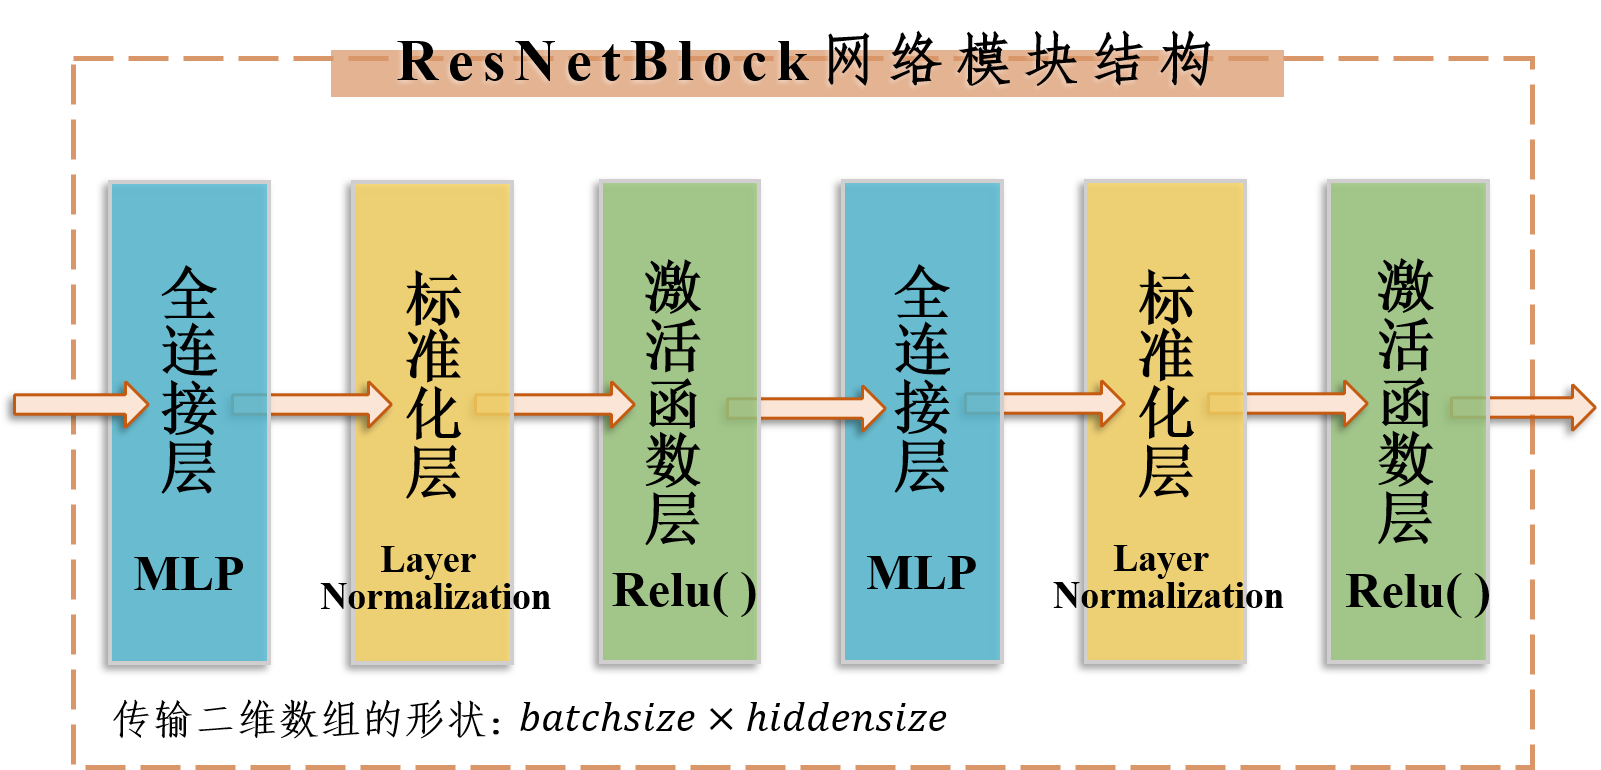
\includegraphics[scale=0.45]{./figs/p5_1.png}
  \caption{残差网络模块的架构}
  \label{残差网络模块}
\end{figure}

该模块的最终的输出结果是第六层的输出与第一层的输入的和, 相对于第六层输出的是期望输出和真实输出之间的残差, 这样的设定使得网络可以学习到残差映射, 同时保留了原始的输入并将其直接传输到了该模块的输出\cite{16,17}. 残差网络中的
跳跃连接能够缓解深层网络下的性能退化与优化困难问题\cite{17}. 标准化层使用了层标准化手段(layer-normlization), 使得输入数据在输出该层时能够具有零均值与单位方差的性质, 同时该标准化手段并不依赖于$batchsize$的大小\cite{19}.
层标准化有效解决了深度网络情况下梯度爆炸与梯度消失的问题. 激活层的$Relu(\,)$的作用是对输入该层的数据逐元素取其正部. 它能够提高计算速率, 使得前向与反向传播的速度更快, 且保留正部而不是压缩数值的激活方式能够缓解梯度消失的问题\cite{20}.

整个神经网络的架构串联拼接了$hidden\_nums$个残差网络模块, 并在串联组前后都添加了一层全连接网络, 输入端还额外添加了一个激活函数$Relu(\,)$层. 图片\ref{网络结构}展示了该模块的架构.

\begin{figure}[H]
  \centering
  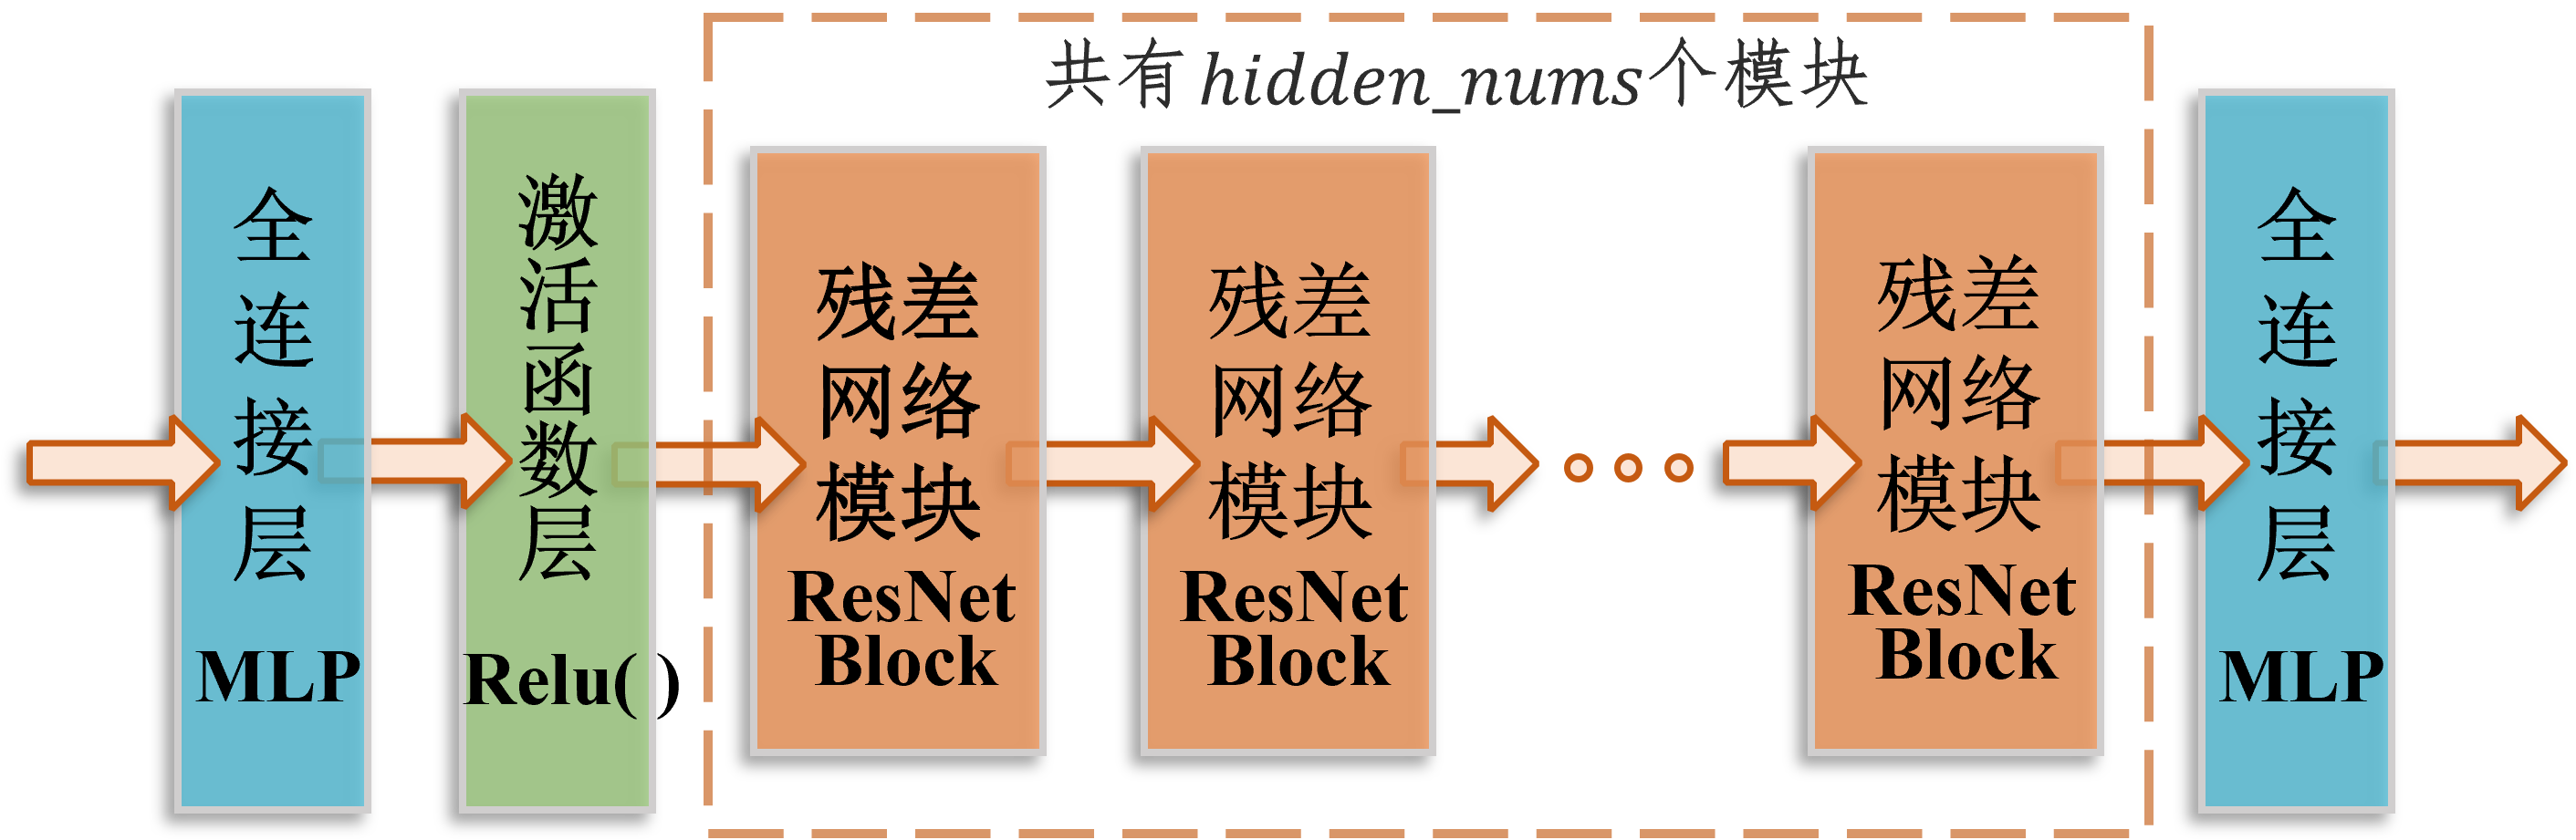
\includegraphics[scale=0.6]{./figs/p5_2.png}
  \caption{本文神经网络模型的结构}
  \label{网络结构}
\end{figure}

\noindent 网络的输入数据形状为$batchsize \times inputsize$, 第一层全连接层的输出数据形状为$batchsize \times hiddensize$, 后续层的输入输出至倒数第一层的输入数据的形状都是$batchsize \times hiddensize$, 最后一层全连接层的输出数据形状为$batchsize \times outputsize$.

对于该章的参数反演神经网络, 其网络模型架构的参数如下:
$$
outputsize = 3, \quad hiddensize = 30, \quad hidden\_nums = 3.
$$
\noindent 整个网络的输出即为反演后的皮肤三参数组, 中间隐藏层的神经元数量为30个, 残差网络模块的串联数量为3个. 同时, 根据特征集的不同, 本节共有两个参数反演神经网络, 两个网络模型的架构只在$inputsize$的取值上有差异. ``血药含量采样28点\&尿药含量采样15点''特征集对应的$inputsize=58$, ``血药含量采样5点\&尿药含量采样5点''特征集对应的$inputsize=15$.

\section[3.4]{参数反演神经网络模型的训练}
\label{3.4}

本章中的两个参数反演神经网络模型的训练部分是相同的, 故不作区分. 
\subsection{数据集的预处理,划分与训练流程}
在训练开始前, 将特征集与标签集分别进行标准化处理, 使作为数据集的矩阵的每一列具有零均值, 单位标准差的性质. 数据集的标准化处理可以增强模型的稳定性, 保持梯度的一致性与稳健性, 减少梯度消失或爆炸的风险\cite{21}. 同时, 标准化处理可以减小数据条目之间的数值差距, 使不同尺度的数据具有类似的分布特性, 令网络训练更专注于反演模型拟合这一主要任务, 而不是专注于输入数据的数值本身. 因而, 在处理未见到的
数据时, 网络也不会因为陌生的数值而给出不佳的表现, 故标准化处理还可以提升网络的泛化能力\cite{22}.

数据集预处理后, 根据训练需求被随机划分为训练集, 验证集, 测试集三个部分, 三个部分的条目比例为$8:1:1$, 特征集与标签集被同步地划分, 划分后依然保持条目一一对应的关系. 

在一轮训练中, 整个训练集被分为若干小批量数据, 在一轮训练内, 每个小批量数据都会前后被代入至未完善模型中,
计算损失函数关于网络模型内各系数的梯度信息, 并根据梯度信息使用优化算法来更新网络模型中的系数\cite{23}. 
利用所有训练集小批量完成了一轮网络模型系数更新后, 将整个验证集分批次地代入至当前的网络模型中, 
观测其对应的损失函数\cite{23}. 在验证期间, 引入早停技术(early stopping)中的耐心值设定: 记录当前有着验证集最优损失的训练轮次, 若接下来连续$patience = 8$个训练轮内验证集上的损失函数没有小于验证集最优损失, 则停止训练并储存当前有着最优验证集损失的网络模型的全部系数, 否则继续下一轮的训练(网络模型系数更新)\cite{23}. 训练结束后, 调用已储存的网络模型, 将验证集内的数据代入至网络模型计算损失函数, 并以此为评价
网络模型优劣的指标之一.

\subsection{损失函数与优化器}

损失函数的设置利用了对偶学习(Dual Learning)的手段, 具体为$\|\vec{\alpha}-\vec{\alpha^*} \|^2$与$\|f(\vec{\alpha})-\tilde{f}(\vec{\alpha^*}) \|^2$的线性组合. 其中
$\vec{\alpha}$为标签皮肤三参数组, $\vec{\alpha^*}$为网络模型输出的反演得到的皮肤三参数组,$f$为公式(\ref{eq2.1})中的PBPK模型的求解模型, $\tilde{f}$为拟合了PBPK模型正向求解的神经网络模型. 由于共有三种化学品含量曲线$A_{plasma}(t), A_{urinebps}(t), A_{urinebpsg}(t)$, 一个参数反演神经网络共对应三个正向拟合神经网络. 每个正向拟合神经网络的输入数据为参数反演网络输出的皮肤三参数组$\vec{\alpha}^*$, 输出的是拟合后的对应于这组皮肤三参数组的某种化学品浓度曲线的采样点, 在下一节会详细介绍对偶学习与PBPK模型拟合神经网络模型的内容. 
以``血药含量采样28点\&尿药含量采样15点''对应的参数反演网络为例, 其损失函数中的$\|f(\vec{\alpha})-\tilde{f}(\vec{\alpha^*}) \|^2$具体形式为

\noindent $(MSE_{plasma}+MSE_{urinebps}+MSE_{urinebpsg})\times \frac{1}{3}$,
其中三个$MSE$分别代表特征集中血药含量曲线采样点与正向拟合神经网络输出的血药含量曲线采样点之间的均方误差, 特征集中尿液BPS累计含量曲线采样点与正向拟合神经网络输出的尿液BPS累计含量曲线采样点之间的均方误差以及特征集中尿液BPS-g累计含量曲线采样点与正向拟合神经网络输出的尿液BPS-g累计含量曲线采样点之间的均方误差.

优化器使用了torch.optim中的Adam(\,)函数, 即Adam算法. 
Adam优化算法中的下降步长需要使用当前梯度信息的一阶矩估计(梯度信息的指数平滑)与二阶矩估计(梯度信息的逐项平方的指数平滑)\cite{24}. 矩估计在经过
修正后(迭代步较小时的矩估计将会被放大), 代入至系数更新公式$\Delta \theta   = -\epsilon \frac{\hat{s}}{\sqrt{\hat{r}} +\delta } $, 其中$\hat{s}$为修正后的一阶矩估计, $\hat{t}$
为修正后的二阶矩估计, $\delta$为用于数值稳定的小常数\cite{24}. Adam算法是一种高效的自适应学习率优化算法, 它可以利用迭代内的历史梯度信息来调整网络模型内每个系数的学习率, 使得模型系数的更新
过程更加灵活与快速\cite{24}. 同时该算法不易陷入局部最优解, 可以很好地处理非凸问题\cite{25}.





\section{对偶学习与PBPK模型拟合神经网络模型}

\subsection{对偶学习的引入背景}
在神经网络的训练过程中, 需要设置损失函数, 并以减少损失函数的数值为目标来迭代网络模型中的系数. 对于参数反演的问题, 见公式(\ref{eq2.1}), 损失函数应设置为$\|f(\vec{\alpha})-f(\vec{\alpha^*}) \|^2 $, 即原本的皮肤三参数组代入至PBPK模型求解得到的含量曲线采样点与网络模型输出的反演皮肤三参数组代入至PBPK模型求解得到的含量曲线采样点之间的平均平方误差. 但由于计算资源问题, 较为庞大的PBPK模型的求解模型难以植入神经网络模型并在反向传播中正常运作. 故损失函数设置为 $\|\vec{\alpha}-\vec{\alpha^*} \|^2 $, 即原本的皮肤三参数组与网络模型输出的反演皮肤三参数组之间的平均平方误差.
但这样的损失函数在训练过程中缺乏对神经网络模型的引导, 此处引入对偶学习, 训练一个能够拟合函数$f$的正向神经网络模型$\tilde{f}$, 与参数反演神经网络形成对偶关系. 同时, 将
$\|f(\vec{\alpha})-\tilde{f}(\vec{\alpha^*}) \|^2 $作为损失函数内的一个正则化项, 与$\|\vec{\alpha}-\vec{\alpha^*} \|^2 $一项共同引导参数反演神经网络去学习$\vec{\alpha}$
与$f(\vec{\alpha})$之间的映射关系. 其中$f(\vec{\alpha})$已知, 即为参数反演神经网络的特征集, $\tilde{f}(\vec{\alpha^*})$是参数反演神经网络输出的皮肤三参数组代入至正向拟合神经网络输出的结果, 含义为
拟合得到的化学品含量曲线上的采样点.

\subsection{正向拟合神经网络模型的数据集结构与构建}
由于与参数反演神经网络是对偶关系, 本章中的正向拟合神经网络也使用固定时间采样节点来构建数据集, 同时也沿用参数反演神经网络数据集内的数据. 由于采样时间节点的不同, 本章共有两种参数反演神经网络, 相应地也有两类正向拟合神经网络.
并且, 为了更好地拟合PBPK模型输出的三种含量曲线$(A_{plasma}(t), A_{urinebps}(t), A_{urinebpsg}(t))$, 对于每种时间采样点, 本节将分别训练三个正向拟合神经网络, 分别拟合血浆BPS含量曲线的采样点,
尿液BPS累计含量曲线的采样点以及尿液BPS-g累计含量曲线的采样点. 故正向拟合神经网络的特征集为皮肤三参数组$\vec{\alpha}$的集合, 对应的标签集为$\vec{\alpha}$代入至PBPK模型求解得到的某种含量曲线的采样点 $(A(t_1),A(t_2),\dots,A(t_n))$的集合.

对于任意一种时间采样点, 需要训练的三个正向拟合神经网络的特征集都与相同时间采样点情形下的参数反演神经网络的标签集相同, 其形状为$44031 \times 3$.
三个正向拟合神经网络的标签集是相同时间采样点情形下的参数反演神经网络的特征集的切片. 例如, 在血药含量曲线采样28点的情况下, 用于拟合$A_{plasma}(t)$曲线的采样点的正向拟合神经网络的标签集是参数反演神经网络的特征集的前28列, 形状即为$44031 \times 28$.

\subsection{正向拟合神经网络模型的网络结构与训练}

本节共有六个正向拟合神经网络, 对应两种时间采样节点与三种含量曲线$(2\times 3 = 6)$. 对于每个正向拟合神经网络, 其架构与图\ref{网络结构}所呈现的相同, 架构中的参数相应地设置为:
$$
inputsize = 3, \quad hiddensize = 30, \quad hidden\_nums = 3.
$$
\noindent 整个网络的输入即为包含44031条皮肤三参数的特征集, 中间隐藏层的神经元数量为30个, 残差网络模块的串联数量为3个. 同时, 根据标签集的不同, 本小节内的六个网络模型的架构只在$outputsize$的取值上有差异. 例如, 用于拟合``血药含量采样28点''的正向拟合神经网络对应的$outputsize=28$.

正向拟合神经网络模型训练时的损失函数为网络输出与对应标签之间的均方误差, 余下的训练方法与流程与\ref{3.4}节中参数反演神经网络模型的训练完全相同, 不再介绍.

\subsection{参数反演神经网络模型的效果展示}

\subsubsection{网络在测试集上的效果}


三参数标签与输出的MAE: 0.2100907415151596
三参数标签与输出的MSE: 0.26290321350097656
三参数标签与输出的MRE: 0.023020707070827484

整个测试集的原始特征与输出三参数通过PBPK模型计算得到的对应采样点的MSE为  5.536357479268417e-06
整个测试集的原始特征与输出三参数通过PBPK模型计算得到的对应采样点的MAE为  0.0008642979384673332
整个测试集的原始特征与输出三参数通过PBPK模型计算得到的对应采样点的MRE为  0.13615118848871022
R^2  0.9989137413239715
R^2  0.9994829772690252

















\clearpage
\mbox{}
\thispagestyle{empty}

\appendix
% 附录部分
\chapter{代码}
\section{代码环境}
\begin{lstlisting}[language=PYTHON]

\end{lstlisting}
\chapter{PBPK模型物理量名称-含义对照表}
\CTEXsetup[format={\Large\bfseries}]{section}
\section*{模型中待求解变量}
\label{app:B}
\noindent$C_{SCi}(t)$  {\hfill 暴露皮肤组织的深度为$i\times \frac{T_{SC}}{10}$的角质层在$t$时刻的BPS浓度$(nmol/cm^3)$}\\
$A_{Fo}(t)$ {\hfill  暴露皮肤组织的毛囊在$t$时刻的BPS含量$(nmol)$}\\
$A_{well}(t)${\hfill 暴露皮肤组织的表皮储仓在$t$时刻的BPS含量$(nmol)$}\\
$A_{VE}(t)${\hfill 暴露皮肤组织的活性表皮在$t$时刻的BPS含量$(nmol)$}\\
$A_{ST}(t)${\hfill 胃部在$t$时刻的BPS含量$(nmol)$}\\
$A_{skin}(t)${\hfill 未暴露皮肤组织在$t$时刻的BPS含量$(nmol)$}\\
$A_{fat}(t)${\hfill 脂肪组织在$t$时刻的BPS含量$(nmol)$}\\
$A_{gonad}(t)${\hfill 性腺在$t$时刻的BPS含量$(nmol)$}\\
$A_{plasma}(t)${\hfill 血浆在$t$时刻的BPS含量$(nmol)$}\\
$A_{brain}(t)${\hfill 脑部在$t$时刻的BPS含量$(nmol)$}\\
$A_{rich}(t)${\hfill 血流丰富组织在$t$时刻的BPS含量$(nmol)$}\\
$A_{slow}(t)${\hfill 血流缓慢组织在$t$时刻的BPS含量$(nmol)$}\\
$A_{GIBPSg}(t)${\hfill 胃肠部在$t$时刻的BPS-g含量$(nmol)$}\\
$A_{GIBPSs}(t)${\hfill 胃肠部在$t$时刻的BPS-s含量$(nmol)$}\\
$A_{SI}(t)${\hfill 小肠在$t$时刻的BPS含量$(nmol)$}\\
$A_{liver}(t)${\hfill 肝脏在$t$时刻的BPS含量$(nmol)$}\\
$A_{BPSg\_delay}(t)${\hfill 发生了肝肠循环的BPS-g的量/小肠在$t$时刻的BPS-g含量$(nmol)$}\\
$A_{BPSs\_delay}(t)${\hfill 发生了肝肠循环的BPS-s的量/小肠在$t$时刻的BPS-s含量$(nmol)$}\\
$A_{BPSg}(t)${\hfill 整个机体在$t$时刻的BPS-g含量$(nmol)$}\\
$A_{BPSs}(t)${\hfill 整个机体在$t$时刻的BPS-s含量$(nmol)$}\\
$A_{urinebps}(t)${\hfill 人体排出的尿液在$t$时刻累计的BPS含量$(nmol)$}\\
$A_{urinebpsg}(t)${\hfill  人体排出的尿液在$t$时刻累计的BPS-g含量$(nmol)$}
\section*{其他变量}
\noindent$\varphi(x,t)${\hfill   暴露皮肤组织的角质层深度x处在$t$时刻的BPS浓度$(nmol/cm^3)$,}\\
$f_1(t)$ {\hfill  皮肤接触外源BPS的量$(nmol)$, 当$t> Time_{add}$时, $f_1(t)=0$}\\
$ON(t)$ {\hfill  布尔值, 当$t\leq Time_{expose}$时, $ON(t)=1$, 皮肤处于BPS暴露状态;}

\hfill 当$t> Time_{expose}$时, $ON(t)=0$, 皮肤处于未暴露状态\\
$f_2(t)$ {\hfill  口服外源BPS的量$(nmol)$, 本文中不考虑口服情况, $f_2(t)=0$}\\

\section*{待反演的参数}
\noindent$DSC$ {\hfill  角质层中的有效扩散系数$(cm^2/h)$}\\
$u_1$ {\hfill  由脱屑而向皮肤表面转移的速度$(cm/min)$}\\
$Pfo$ {\hfill  毛囊的渗透系数$(cm/h)$}

\section*{理化数据中的常量}
\noindent$T_{SC}$ {\hfill  角质层的深度$(um)$}\\
$SCDX$ {\hfill  角质层的深度的$\frac{1}{10}(um)$}\\
$HSC_{well}$ {\hfill  角质层和皮肤表皮储仓之间的分配系数}\\
$V_{well}$ {\hfill  暴露皮肤组织的表面储仓体积$(L)$}\\
$HSC_{VE}$ {\hfill  角质层和活性表皮之间的分配系数}\\
$V_{TVE}$ {\hfill  暴露皮肤组织的活性表皮层体积$(L)$}\\
$AEXP $ {\hfill  暴露皮肤组织面积$ (dm^2)$}\\
$ FEXP$ {\hfill  暴露皮肤组织中毛囊的面积分数}\\
$HFo_{well}$ {\hfill  毛囊和皮肤表皮储仓之间的分配系数}\\
$V_{TFo}$ {\hfill  暴露皮肤组织的毛囊体积$(L)$}\\
$ Qskin$ {\hfill  皮肤血液流速$(L/h) $}\\
$ pskin$ {\hfill  皮肤-血浆分配系数}\\
$ BSA$ {\hfill  人体皮肤表面积$(dm^2) $}\\
$V_{plasma}$ {\hfill  血浆体积$(L)$}\\
$k0 $ {\hfill  口服给药时BPS从胃进入肝脏的系数$(h^{-1})$}\\
$k1 $ {\hfill  口服给药时BPS从小肠进入肝脏的系数$(h^{-1})$}\\
$ ge$ {\hfill  口服给药时BPS由胃转移至小肠的系数$(h^{-1})$}\\
$V_{TSC}$ {\hfill  暴露皮肤组织的角质层体积$(L)$}\\
$V_{skin}$ {\hfill  皮肤组织的体积$(L)$}\\
$ Qfat$ {\hfill  脂肪组织血液流速$(L/h) $}\\
$V_{fat}$ {\hfill  脂肪组织的体积$(L)$}\\
$ pfat$ {\hfill  脂肪-血浆分配系数}\\
$ Qgonad$ {\hfill  性腺血液流速$(L/h) $}\\
$V_{gonad}$ {\hfill  性腺的体积$(L)$}\\
$ pgonad$ {\hfill  性腺-血浆分配系数}\\
$ Kurinebps $ {\hfill  BPS尿液排泄参数$(L/h)$}\\
$ Qc$ {\hfill  心脏血液流速$(L/h)$}\\
$ Qbrain$ {\hfill  脑部血液流速$(L/h) $}\\
$V_{brain}$ {\hfill  脑部的体积$(L)$}\\
$ pbrain$ {\hfill  脑部-血浆分配系数}\\
$ Qrich$ {\hfill  血流丰富组织血液流速$(L/h) $}\\
$V_{rich}$ {\hfill  血流丰富组织的体积$(L)$}\\
$ prich$ {\hfill  血流丰富组织-血浆分配系数}\\
$ Qslow$ {\hfill  血流缓慢组织血液流速$(L/h) $}\\
$V_{slow}$ {\hfill  血流缓慢组织的体积$(L)$}\\
$ pslow$ {\hfill  血流缓慢组织-血浆分配系数}\\
$ Qliver$ {\hfill  肝脏血液流速$(L/h) $}\\
$V_{liver}$ {\hfill  肝脏的体积$(L)$}\\
$ pliver$ {\hfill  肝脏-血浆分配系数}\\
$kGIing$ {\hfill 口服给药BPS-g从肠到血中的系数 $(h^{-1})$}\\
$kGIins $ {\hfill  口服给药BPS-s从肠到血中的系数 $(h^{-1})$}\\
$Vmaxgutg$ {\hfill  肠道中BPS葡萄苷酸化的最大反应速度$(nmol/h)$}\\
$Vmaxguts$ {\hfill  肠道中BPS硫酸盐化的最大反应速度$(nmol/h)$}\\
$enterocytes $ {\hfill  小肠体积$(L)$}\\
$ Kmgutg$ {\hfill  肠道中BPS葡萄苷酸化的米氏常数$(nmol)$}\\
$ Kmguts$ {\hfill  肠道中BPS硫酸盐化的米氏常数$(nmol)$}\\
$ Ksigutg$ {\hfill  肠道中葡萄苷酸化结合底物抑制常数$(nmol)$}\\
$ kenterobpsg$ {\hfill  BPS-g肝肠循环使得BPS发生循环的速率$(h^{-1})$}\\
$ kenterobpss$ {\hfill  BPS-s肝肠循环使得BPS发生循环的速率$(h^{-1})$}\\
$ Kmliverg$ {\hfill  肝脏中BPS葡萄苷酸化的米氏常数$(nmol)$}\\
$Vmaxliverg$ {\hfill  肠道中BPS葡萄苷酸化的最大反应速度$(nmol/h)$}\\
$ Kmlivers$ {\hfill  肝脏中BPS硫酸盐化的米氏常数$(nmol)$}\\
$Vmaxlivers$ {\hfill  肠道中BPS硫酸盐化的最大反应速度$(nmol/h)$}\\
$met1g $ {\hfill  肝脏中BPS-g进入血液中的比例}\\
$ met1s$ {\hfill  肝脏中BPS-s进入血液中的比例}\\
$met2g = 1 -  met1g$ {\hfill  肝脏中BPS-g进入肝肠循环的比例}\\
$ met2s= 1 -  met1s$ {\hfill  肝脏中BPS-s进入肝肠循环的比例}\\
$ kentero$ {\hfill  BPS-g肝肠循环的速率$(h^{-1})$}\\
$k4_{IV} $ {\hfill  BPS-g在肝肠循环中的粪便消除系数$(h^{-1})$}\\
$ Kurinebpsg$ {\hfill  BPS-g的尿液排泄参数$(L/h)$}\\
$Vbodyg  $ {\hfill  参与BPS-g分布的组织体积$(L)$}\\
$ Kurinebpss$ {\hfill  BPS-s的尿液排泄参数$(L/h)$}\\
$ Vbodys$ {\hfill  参与BPS-s分布的组织体积$(L)$}

\section*{实验设置的常量}
\noindent$Time_{add}=\frac{1}{6}h$ {\hfill  手指皮肤触摸热敏纸(外源BPS)的时间$(h)$}\\
$Time_{expose}=\frac{13}{6}h$ {\hfill  手指皮肤表皮储仓内BPS含量大于0的时间$(h)$}\\
\clearpage
\mbox{}
\thispagestyle{empty}

% 引用部分
\bibliography{REF}
% \bibliographystyle{authoryear}


% 引用过的文献会自动进入这一部分,如果有文献未引用但也想放入参考文献,请使用以下命令
% \nocite{请填入文献代码}
% 需要使用其它格式时请将该句取消注释.
\addcontentsline{toc}{chapter}{参考文献}
% 将参考文献加入目录

\clearpage
\mbox{}
\thispagestyle{empty}

\chapter*{致\quad 谢}
\addcontentsline{toc}{chapter}{致谢}
% 将致谢加入目录
\normalsize
致谢


\end{document}

